\documentclass[11pt]{article}
\usepackage[margin=1in]{geometry}
\usepackage[T1]{fontenc}
\usepackage{lmodern}
\usepackage{amsmath,amssymb,booktabs,array,graphicx}
\usepackage[round]{natbib}
\usepackage[section]{placeins}
\usepackage[hidelinks]{hyperref}
\emergencystretch=3em

% Result numbers. Generated by `crew.py numbers`; never typed by hand.
% Generated by `crew.py numbers` from claims.jsonl. Do not edit by hand.
% Each macro is a number taken from a logged run; see claims.jsonl.
\newcommand{\HOneAdultMean}{0.0033}  % r-h1-adult-mean
\newcommand{\HOneAdultLo}{-0.0001}  % r-h1-adult-lo
\newcommand{\HOneAdultHi}{0.0068}  % r-h1-adult-hi
\newcommand{\HOneAdultCat}{3}  % r-h1-adult-cat
\newcommand{\HOneBankMean}{-0.0147}  % r-h1-bank-marketing-mean
\newcommand{\HOneBankLo}{-0.0161}  % r-h1-bank-marketing-lo
\newcommand{\HOneBankHi}{-0.0134}  % r-h1-bank-marketing-hi
\newcommand{\HOneBankCat}{2}  % r-h1-bank-marketing-cat
\newcommand{\HOneElecMean}{0.0270}  % r-h1-electricity-mean
\newcommand{\HOneElecLo}{0.0232}  % r-h1-electricity-lo
\newcommand{\HOneElecHi}{0.0308}  % r-h1-electricity-hi
\newcommand{\HOneElecCat}{1}  % r-h1-electricity-cat
\newcommand{\HOnePhonemeMean}{-0.0263}  % r-h1-phoneme-mean
\newcommand{\HOnePhonemeLo}{-0.0339}  % r-h1-phoneme-lo
\newcommand{\HOnePhonemeHi}{-0.0187}  % r-h1-phoneme-hi
\newcommand{\HOnePhonemeCat}{2}  % r-h1-phoneme-cat
\newcommand{\HOneOverallCode}{2}  % r-h1-overall
\newcommand{\HTwoAAdultMean}{0.0003}  % r-h2a-adult-mean
\newcommand{\HTwoAAdultLo}{-0.0001}  % r-h2a-adult-lo
\newcommand{\HTwoAAdultHi}{0.0007}  % r-h2a-adult-hi
\newcommand{\HTwoAAdultCat}{0}  % r-h2a-adult-cat
\newcommand{\HTwoABankMean}{-0.0000}  % r-h2a-bank-marketing-mean
\newcommand{\HTwoABankLo}{-0.0003}  % r-h2a-bank-marketing-lo
\newcommand{\HTwoABankHi}{0.0002}  % r-h2a-bank-marketing-hi
\newcommand{\HTwoABankCat}{0}  % r-h2a-bank-marketing-cat
\newcommand{\HTwoAElecMean}{-0.0028}  % r-h2a-electricity-mean
\newcommand{\HTwoAElecLo}{-0.0030}  % r-h2a-electricity-lo
\newcommand{\HTwoAElecHi}{-0.0025}  % r-h2a-electricity-hi
\newcommand{\HTwoAElecCat}{1}  % r-h2a-electricity-cat
\newcommand{\HTwoAPhonemeMean}{-0.0007}  % r-h2a-phoneme-mean
\newcommand{\HTwoAPhonemeLo}{-0.0018}  % r-h2a-phoneme-lo
\newcommand{\HTwoAPhonemeHi}{0.0005}  % r-h2a-phoneme-hi
\newcommand{\HTwoAPhonemeCat}{3}  % r-h2a-phoneme-cat
\newcommand{\HTwoAOverallCode}{3}  % r-h2a-overall
\newcommand{\HTwoBAdultMean}{0.0002}  % r-h2b-adult-mean
\newcommand{\HTwoBAdultLo}{0.0001}  % r-h2b-adult-lo
\newcommand{\HTwoBAdultHi}{0.0004}  % r-h2b-adult-hi
\newcommand{\HTwoBAdultCat}{0}  % r-h2b-adult-cat
\newcommand{\HTwoBBankMean}{-0.0005}  % r-h2b-bank-marketing-mean
\newcommand{\HTwoBBankLo}{-0.0008}  % r-h2b-bank-marketing-lo
\newcommand{\HTwoBBankHi}{-0.0002}  % r-h2b-bank-marketing-hi
\newcommand{\HTwoBBankCat}{0}  % r-h2b-bank-marketing-cat
\newcommand{\HTwoBElecMean}{-0.0004}  % r-h2b-electricity-mean
\newcommand{\HTwoBElecLo}{-0.0007}  % r-h2b-electricity-lo
\newcommand{\HTwoBElecHi}{-0.0002}  % r-h2b-electricity-hi
\newcommand{\HTwoBElecCat}{0}  % r-h2b-electricity-cat
\newcommand{\HTwoBPhonemeMean}{0.0006}  % r-h2b-phoneme-mean
\newcommand{\HTwoBPhonemeLo}{-0.0001}  % r-h2b-phoneme-lo
\newcommand{\HTwoBPhonemeHi}{0.0014}  % r-h2b-phoneme-hi
\newcommand{\HTwoBPhonemeCat}{3}  % r-h2b-phoneme-cat
\newcommand{\HTwoBOverallCode}{0}  % r-h2b-overall
\newcommand{\HOneDbAdultMean}{0.0042}  % r-h1db-adult-mean
\newcommand{\HOneDbAdultLo}{0.0002}  % r-h1db-adult-lo
\newcommand{\HOneDbAdultHi}{0.0082}  % r-h1db-adult-hi
\newcommand{\HOneDbAdultCat}{1}  % r-h1db-adult-cat
\newcommand{\HOneDbBankMean}{-0.0160}  % r-h1db-bank-marketing-mean
\newcommand{\HOneDbBankLo}{-0.0173}  % r-h1db-bank-marketing-lo
\newcommand{\HOneDbBankHi}{-0.0147}  % r-h1db-bank-marketing-hi
\newcommand{\HOneDbBankCat}{2}  % r-h1db-bank-marketing-cat
\newcommand{\HOneDbElecMean}{0.0322}  % r-h1db-electricity-mean
\newcommand{\HOneDbElecLo}{0.0275}  % r-h1db-electricity-lo
\newcommand{\HOneDbElecHi}{0.0369}  % r-h1db-electricity-hi
\newcommand{\HOneDbElecCat}{1}  % r-h1db-electricity-cat
\newcommand{\HOneDbPhonemeMean}{-0.0235}  % r-h1db-phoneme-mean
\newcommand{\HOneDbPhonemeLo}{-0.0329}  % r-h1db-phoneme-lo
\newcommand{\HOneDbPhonemeHi}{-0.0142}  % r-h1db-phoneme-hi
\newcommand{\HOneDbPhonemeCat}{2}  % r-h1db-phoneme-cat
\newcommand{\HOneDbOverallCode}{2}  % r-h1db-overall
\newcommand{\HTwoANcalAdultMean}{0.0009}  % r-h2a_ncal-adult-mean
\newcommand{\HTwoANcalAdultLo}{0.0005}  % r-h2a_ncal-adult-lo
\newcommand{\HTwoANcalAdultHi}{0.0012}  % r-h2a_ncal-adult-hi
\newcommand{\HTwoANcalAdultCat}{2}  % r-h2a_ncal-adult-cat
\newcommand{\HTwoANcalBankMean}{0.0008}  % r-h2a_ncal-bank-marketing-mean
\newcommand{\HTwoANcalBankLo}{0.0006}  % r-h2a_ncal-bank-marketing-lo
\newcommand{\HTwoANcalBankHi}{0.0011}  % r-h2a_ncal-bank-marketing-hi
\newcommand{\HTwoANcalBankCat}{2}  % r-h2a_ncal-bank-marketing-cat
\newcommand{\HTwoANcalElecMean}{-0.0022}  % r-h2a_ncal-electricity-mean
\newcommand{\HTwoANcalElecLo}{-0.0026}  % r-h2a_ncal-electricity-lo
\newcommand{\HTwoANcalElecHi}{-0.0018}  % r-h2a_ncal-electricity-hi
\newcommand{\HTwoANcalElecCat}{1}  % r-h2a_ncal-electricity-cat
\newcommand{\HTwoANcalOverallCode}{2}  % r-h2a-ncal-overall
\newcommand{\HTwoBNcalAdultMean}{0.0010}  % r-h2b_ncal-adult-mean
\newcommand{\HTwoBNcalAdultLo}{0.0007}  % r-h2b_ncal-adult-lo
\newcommand{\HTwoBNcalAdultHi}{0.0013}  % r-h2b_ncal-adult-hi
\newcommand{\HTwoBNcalAdultCat}{2}  % r-h2b_ncal-adult-cat
\newcommand{\HTwoBNcalBankMean}{0.0001}  % r-h2b_ncal-bank-marketing-mean
\newcommand{\HTwoBNcalBankLo}{-0.0004}  % r-h2b_ncal-bank-marketing-lo
\newcommand{\HTwoBNcalBankHi}{0.0006}  % r-h2b_ncal-bank-marketing-hi
\newcommand{\HTwoBNcalBankCat}{0}  % r-h2b_ncal-bank-marketing-cat
\newcommand{\HTwoBNcalElecMean}{0.0001}  % r-h2b_ncal-electricity-mean
\newcommand{\HTwoBNcalElecLo}{-0.0002}  % r-h2b_ncal-electricity-lo
\newcommand{\HTwoBNcalElecHi}{0.0004}  % r-h2b_ncal-electricity-hi
\newcommand{\HTwoBNcalElecCat}{0}  % r-h2b_ncal-electricity-cat
\newcommand{\HTwoBNcalOverallCode}{3}  % r-h2b-ncal-overall
\newcommand{\HOneTimeElecMean}{0.0008}  % r-h1_time-electricity-mean
\newcommand{\HOneTimeElecLo}{-0.0100}  % r-h1_time-electricity-lo
\newcommand{\HOneTimeElecHi}{0.0116}  % r-h1_time-electricity-hi
\newcommand{\HOneTimeElecCat}{3}  % r-h1_time-electricity-cat
\newcommand{\HTwoATimeElecMean}{0.0265}  % r-h2a_time-electricity-mean
\newcommand{\HTwoATimeElecLo}{0.0209}  % r-h2a_time-electricity-lo
\newcommand{\HTwoATimeElecHi}{0.0322}  % r-h2a_time-electricity-hi
\newcommand{\HTwoATimeElecCat}{2}  % r-h2a_time-electricity-cat
\newcommand{\HTwoBTimeElecMean}{-0.0782}  % r-h2b_time-electricity-mean
\newcommand{\HTwoBTimeElecLo}{-0.1013}  % r-h2b_time-electricity-lo
\newcommand{\HTwoBTimeElecHi}{-0.0551}  % r-h2b_time-electricity-hi
\newcommand{\HTwoBTimeElecCat}{1}  % r-h2b_time-electricity-cat
\newcommand{\ElecTimeLrNoneEce}{0.1677}  % r-time-lr-none-ece-mean
\newcommand{\ElecTimeLrNoneEceSd}{0.0057}  % r-time-lr-none-ece-sd
\newcommand{\ElecTimeLrNoneBrier}{0.2018}  % r-time-lr-none-brier-mean
\newcommand{\ElecTimeLrNoneBrierSd}{0.0031}  % r-time-lr-none-brier-sd
\newcommand{\ElecTimeLrNoneAuc}{0.841}  % r-time-lr-none-auc-mean
\newcommand{\ElecTimeLrNoneAucSd}{0.0035}  % r-time-lr-none-auc-sd
\newcommand{\ElecTimeLrPlattEce}{0.2785}  % r-time-lr-platt-ece-mean
\newcommand{\ElecTimeLrPlattEceSd}{0.0052}  % r-time-lr-platt-ece-sd
\newcommand{\ElecTimeLrPlattBrier}{0.2509}  % r-time-lr-platt-brier-mean
\newcommand{\ElecTimeLrPlattBrierSd}{0.0026}  % r-time-lr-platt-brier-sd
\newcommand{\ElecTimeLrPlattAuc}{0.841}  % r-time-lr-platt-auc-mean
\newcommand{\ElecTimeLrPlattAucSd}{0.0035}  % r-time-lr-platt-auc-sd
\newcommand{\ElecTimeLrIsoEce}{0.2621}  % r-time-lr-isotonic-ece-mean
\newcommand{\ElecTimeLrIsoEceSd}{0.0074}  % r-time-lr-isotonic-ece-sd
\newcommand{\ElecTimeLrIsoBrier}{0.2531}  % r-time-lr-isotonic-brier-mean
\newcommand{\ElecTimeLrIsoBrierSd}{0.0030}  % r-time-lr-isotonic-brier-sd
\newcommand{\ElecTimeLrIsoAuc}{0.817}  % r-time-lr-isotonic-auc-mean
\newcommand{\ElecTimeLrIsoAucSd}{0.0110}  % r-time-lr-isotonic-auc-sd
\newcommand{\ElecTimeRfNoneEce}{0.1685}  % r-time-rf-none-ece-mean
\newcommand{\ElecTimeRfNoneEceSd}{0.0156}  % r-time-rf-none-ece-sd
\newcommand{\ElecTimeRfNoneBrier}{0.1971}  % r-time-rf-none-brier-mean
\newcommand{\ElecTimeRfNoneBrierSd}{0.0046}  % r-time-rf-none-brier-sd
\newcommand{\ElecTimeRfNoneAuc}{0.828}  % r-time-rf-none-auc-mean
\newcommand{\ElecTimeRfNoneAucSd}{0.0046}  % r-time-rf-none-auc-sd
\newcommand{\ElecTimeRfPlattEce}{0.1975}  % r-time-rf-platt-ece-mean
\newcommand{\ElecTimeRfPlattEceSd}{0.0157}  % r-time-rf-platt-ece-sd
\newcommand{\ElecTimeRfPlattBrier}{0.2091}  % r-time-rf-platt-brier-mean
\newcommand{\ElecTimeRfPlattBrierSd}{0.0072}  % r-time-rf-platt-brier-sd
\newcommand{\ElecTimeRfPlattAuc}{0.828}  % r-time-rf-platt-auc-mean
\newcommand{\ElecTimeRfPlattAucSd}{0.0046}  % r-time-rf-platt-auc-sd
\newcommand{\ElecTimeRfIsoEce}{0.2050}  % r-time-rf-isotonic-ece-mean
\newcommand{\ElecTimeRfIsoEceSd}{0.0112}  % r-time-rf-isotonic-ece-sd
\newcommand{\ElecTimeRfIsoBrier}{0.2236}  % r-time-rf-isotonic-brier-mean
\newcommand{\ElecTimeRfIsoBrierSd}{0.0069}  % r-time-rf-isotonic-brier-sd
\newcommand{\ElecTimeRfIsoAuc}{0.817}  % r-time-rf-isotonic-auc-mean
\newcommand{\ElecTimeRfIsoAucSd}{0.0067}  % r-time-rf-isotonic-auc-sd
\newcommand{\ElecTimeHgbNoneEce}{0.3339}  % r-time-hgb-none-ece-mean
\newcommand{\ElecTimeHgbNoneEceSd}{0.0270}  % r-time-hgb-none-ece-sd
\newcommand{\ElecTimeHgbNoneBrier}{0.3271}  % r-time-hgb-none-brier-mean
\newcommand{\ElecTimeHgbNoneBrierSd}{0.0274}  % r-time-hgb-none-brier-sd
\newcommand{\ElecTimeHgbNoneAuc}{0.841}  % r-time-hgb-none-auc-mean
\newcommand{\ElecTimeHgbNoneAucSd}{0.0085}  % r-time-hgb-none-auc-sd
\newcommand{\ElecTimeHgbPlattEce}{0.2456}  % r-time-hgb-platt-ece-mean
\newcommand{\ElecTimeHgbPlattEceSd}{0.0180}  % r-time-hgb-platt-ece-sd
\newcommand{\ElecTimeHgbPlattBrier}{0.2453}  % r-time-hgb-platt-brier-mean
\newcommand{\ElecTimeHgbPlattBrierSd}{0.0148}  % r-time-hgb-platt-brier-sd
\newcommand{\ElecTimeHgbPlattAuc}{0.841}  % r-time-hgb-platt-auc-mean
\newcommand{\ElecTimeHgbPlattAucSd}{0.0085}  % r-time-hgb-platt-auc-sd
\newcommand{\ElecTimeHgbIsoEce}{0.2406}  % r-time-hgb-isotonic-ece-mean
\newcommand{\ElecTimeHgbIsoEceSd}{0.0119}  % r-time-hgb-isotonic-ece-sd
\newcommand{\ElecTimeHgbIsoBrier}{0.2489}  % r-time-hgb-isotonic-brier-mean
\newcommand{\ElecTimeHgbIsoBrierSd}{0.0105}  % r-time-hgb-isotonic-brier-sd
\newcommand{\ElecTimeHgbIsoAuc}{0.813}  % r-time-hgb-isotonic-auc-mean
\newcommand{\ElecTimeHgbIsoAucSd}{0.0140}  % r-time-hgb-isotonic-auc-sd
\newcommand{\TimeVicfillTrainMin}{7642}  % r-time-vicfill-train-min
\newcommand{\TimeVicfillTrainMax}{7753}  % r-time-vicfill-train-max
\newcommand{\TimeVicfillCalMin}{0}  % r-time-vicfill-cal-min
\newcommand{\TimeVicfillCalMax}{0}  % r-time-vicfill-cal-max
\newcommand{\TimeVicfillTestMin}{0}  % r-time-vicfill-test-min
\newcommand{\TimeVicfillTestMax}{0}  % r-time-vicfill-test-max
\newcommand{\MainVicfillTrainMean}{3854}  % r-main-vicfill-train-mean
\newcommand{\MainVicfillCalMean}{1918}  % r-main-vicfill-cal-mean
\newcommand{\MainVicfillTestMean}{1928}  % r-main-vicfill-test-mean
\newcommand{\AdultLrNoneEce}{0.0134}  % r-mean-adult-lr-none-ece
\newcommand{\AdultLrNoneEceSd}{0.0025}  % r-sd-adult-lr-none-ece
\newcommand{\AdultLrNoneEceDb}{0.0088}  % r-mean-adult-lr-none-ecedb
\newcommand{\AdultLrNoneEceDbSd}{0.0035}  % r-sd-adult-lr-none-ecedb
\newcommand{\AdultLrNoneBrier}{0.1023}  % r-mean-adult-lr-none-brier
\newcommand{\AdultLrNoneBrierSd}{0.0028}  % r-sd-adult-lr-none-brier
\newcommand{\AdultLrPlattEce}{0.0129}  % r-mean-adult-lr-platt-ece
\newcommand{\AdultLrPlattEceSd}{0.0024}  % r-sd-adult-lr-platt-ece
\newcommand{\AdultLrPlattEceDb}{0.0081}  % r-mean-adult-lr-platt-ecedb
\newcommand{\AdultLrPlattEceDbSd}{0.0032}  % r-sd-adult-lr-platt-ecedb
\newcommand{\AdultLrPlattBrier}{0.1023}  % r-mean-adult-lr-platt-brier
\newcommand{\AdultLrPlattBrierSd}{0.0028}  % r-sd-adult-lr-platt-brier
\newcommand{\AdultLrIsoEce}{0.0173}  % r-mean-adult-lr-isotonic-ece
\newcommand{\AdultLrIsoEceSd}{0.0054}  % r-sd-adult-lr-isotonic-ece
\newcommand{\AdultLrIsoEceDb}{0.0138}  % r-mean-adult-lr-isotonic-ecedb
\newcommand{\AdultLrIsoEceDbSd}{0.0063}  % r-sd-adult-lr-isotonic-ecedb
\newcommand{\AdultLrIsoBrier}{0.1031}  % r-mean-adult-lr-isotonic-brier
\newcommand{\AdultLrIsoBrierSd}{0.0028}  % r-sd-adult-lr-isotonic-brier
\newcommand{\AdultLrNoneLogloss}{0.320}  % r-mean-adult-lr-none-logloss
\newcommand{\AdultLrNoneLoglossSd}{0.0089}  % r-sd-adult-lr-none-logloss
\newcommand{\AdultLrNoneAuc}{0.905}  % r-mean-adult-lr-none-auc
\newcommand{\AdultLrNoneAucSd}{0.0059}  % r-sd-adult-lr-none-auc
\newcommand{\AdultLrIsoLogloss}{0.325}  % r-mean-adult-lr-isotonic-logloss
\newcommand{\AdultLrIsoLoglossSd}{0.0100}  % r-sd-adult-lr-isotonic-logloss
\newcommand{\AdultLrIsoAuc}{0.904}  % r-mean-adult-lr-isotonic-auc
\newcommand{\AdultLrIsoAucSd}{0.0058}  % r-sd-adult-lr-isotonic-auc
\newcommand{\AdultRfNoneEce}{0.0168}  % r-mean-adult-rf-none-ece
\newcommand{\AdultRfNoneEceSd}{0.0052}  % r-sd-adult-rf-none-ece
\newcommand{\AdultRfNoneEceDb}{0.0130}  % r-mean-adult-rf-none-ecedb
\newcommand{\AdultRfNoneEceDbSd}{0.0063}  % r-sd-adult-rf-none-ecedb
\newcommand{\AdultRfNoneBrier}{0.1041}  % r-mean-adult-rf-none-brier
\newcommand{\AdultRfNoneBrierSd}{0.0024}  % r-sd-adult-rf-none-brier
\newcommand{\AdultRfPlattEce}{0.0162}  % r-mean-adult-rf-platt-ece
\newcommand{\AdultRfPlattEceSd}{0.0053}  % r-sd-adult-rf-platt-ece
\newcommand{\AdultRfPlattEceDb}{0.0120}  % r-mean-adult-rf-platt-ecedb
\newcommand{\AdultRfPlattEceDbSd}{0.0065}  % r-sd-adult-rf-platt-ecedb
\newcommand{\AdultRfPlattBrier}{0.1041}  % r-mean-adult-rf-platt-brier
\newcommand{\AdultRfPlattBrierSd}{0.0022}  % r-sd-adult-rf-platt-brier
\newcommand{\AdultRfIsoEce}{0.0157}  % r-mean-adult-rf-isotonic-ece
\newcommand{\AdultRfIsoEceSd}{0.0049}  % r-sd-adult-rf-isotonic-ece
\newcommand{\AdultRfIsoEceDb}{0.0119}  % r-mean-adult-rf-isotonic-ecedb
\newcommand{\AdultRfIsoEceDbSd}{0.0060}  % r-sd-adult-rf-isotonic-ecedb
\newcommand{\AdultRfIsoBrier}{0.1044}  % r-mean-adult-rf-isotonic-brier
\newcommand{\AdultRfIsoBrierSd}{0.0023}  % r-sd-adult-rf-isotonic-brier
\newcommand{\AdultRfNoneLogloss}{0.338}  % r-mean-adult-rf-none-logloss
\newcommand{\AdultRfNoneLoglossSd}{0.0114}  % r-sd-adult-rf-none-logloss
\newcommand{\AdultRfNoneAuc}{0.899}  % r-mean-adult-rf-none-auc
\newcommand{\AdultRfNoneAucSd}{0.0052}  % r-sd-adult-rf-none-auc
\newcommand{\AdultRfIsoLogloss}{0.331}  % r-mean-adult-rf-isotonic-logloss
\newcommand{\AdultRfIsoLoglossSd}{0.0065}  % r-sd-adult-rf-isotonic-logloss
\newcommand{\AdultRfIsoAuc}{0.898}  % r-mean-adult-rf-isotonic-auc
\newcommand{\AdultRfIsoAucSd}{0.0052}  % r-sd-adult-rf-isotonic-auc
\newcommand{\AdultHgbNoneEce}{0.0132}  % r-mean-adult-hgb-none-ece
\newcommand{\AdultHgbNoneEceSd}{0.0025}  % r-sd-adult-hgb-none-ece
\newcommand{\AdultHgbNoneEceDb}{0.0094}  % r-mean-adult-hgb-none-ecedb
\newcommand{\AdultHgbNoneEceDbSd}{0.0035}  % r-sd-adult-hgb-none-ecedb
\newcommand{\AdultHgbNoneBrier}{0.0913}  % r-mean-adult-hgb-none-brier
\newcommand{\AdultHgbNoneBrierSd}{0.0021}  % r-sd-adult-hgb-none-brier
\newcommand{\AdultHgbPlattEce}{0.0115}  % r-mean-adult-hgb-platt-ece
\newcommand{\AdultHgbPlattEceSd}{0.0013}  % r-sd-adult-hgb-platt-ece
\newcommand{\AdultHgbPlattEceDb}{0.0069}  % r-mean-adult-hgb-platt-ecedb
\newcommand{\AdultHgbPlattEceDbSd}{0.0016}  % r-sd-adult-hgb-platt-ecedb
\newcommand{\AdultHgbPlattBrier}{0.0913}  % r-mean-adult-hgb-platt-brier
\newcommand{\AdultHgbPlattBrierSd}{0.0020}  % r-sd-adult-hgb-platt-brier
\newcommand{\AdultHgbIsoEce}{0.0130}  % r-mean-adult-hgb-isotonic-ece
\newcommand{\AdultHgbIsoEceSd}{0.0032}  % r-sd-adult-hgb-isotonic-ece
\newcommand{\AdultHgbIsoEceDb}{0.0093}  % r-mean-adult-hgb-isotonic-ecedb
\newcommand{\AdultHgbIsoEceDbSd}{0.0043}  % r-sd-adult-hgb-isotonic-ecedb
\newcommand{\AdultHgbIsoBrier}{0.0916}  % r-mean-adult-hgb-isotonic-brier
\newcommand{\AdultHgbIsoBrierSd}{0.0020}  % r-sd-adult-hgb-isotonic-brier
\newcommand{\AdultHgbNoneLogloss}{0.289}  % r-mean-adult-hgb-none-logloss
\newcommand{\AdultHgbNoneLoglossSd}{0.0062}  % r-sd-adult-hgb-none-logloss
\newcommand{\AdultHgbNoneAuc}{0.922}  % r-mean-adult-hgb-none-auc
\newcommand{\AdultHgbNoneAucSd}{0.0037}  % r-sd-adult-hgb-none-auc
\newcommand{\AdultHgbIsoLogloss}{0.293}  % r-mean-adult-hgb-isotonic-logloss
\newcommand{\AdultHgbIsoLoglossSd}{0.0067}  % r-sd-adult-hgb-isotonic-logloss
\newcommand{\AdultHgbIsoAuc}{0.921}  % r-mean-adult-hgb-isotonic-auc
\newcommand{\AdultHgbIsoAucSd}{0.0038}  % r-sd-adult-hgb-isotonic-auc
\newcommand{\AdultLrNoneEceBins}{15.0}  % r-bins-adult-lr-none
\newcommand{\AdultRfNoneEceBins}{13.0}  % r-bins-adult-rf-none
\newcommand{\AdultHgbNoneEceBins}{15.0}  % r-bins-adult-hgb-none
\newcommand{\AdultRfNoneClipLow}{1056}  % r-clip-adult-rf-none
\newcommand{\AdultRfMinusLrBrierMean}{0.0017}  % r-rfminuslr-adult-brier-mean
\newcommand{\AdultRfMinusLrBrierLo}{0.0003}  % r-rfminuslr-adult-brier-lo
\newcommand{\AdultRfMinusLrBrierHi}{0.0032}  % r-rfminuslr-adult-brier-hi
\newcommand{\AdultRfMinusLrLoglossMean}{0.0178}  % r-rfminuslr-adult-logloss-mean
\newcommand{\AdultRfMinusLrLoglossLo}{0.0122}  % r-rfminuslr-adult-logloss-lo
\newcommand{\AdultRfMinusLrLoglossHi}{0.0235}  % r-rfminuslr-adult-logloss-hi
\newcommand{\AdultLrPlattMinusNoneBrierMean}{-0.0000}  % r-plattminusnone-adult-lr-brier-mean
\newcommand{\AdultLrPlattMinusNoneBrierLo}{-0.0001}  % r-plattminusnone-adult-lr-brier-lo
\newcommand{\AdultLrPlattMinusNoneBrierHi}{0.0000}  % r-plattminusnone-adult-lr-brier-hi
\newcommand{\AdultLrIsoMinusPlattAuc}{-0.0012}  % r-isominusplatt-adult-lr-auc
\newcommand{\AdultRfPlattMinusNoneBrierMean}{-0.0000}  % r-plattminusnone-adult-rf-brier-mean
\newcommand{\AdultRfPlattMinusNoneBrierLo}{-0.0003}  % r-plattminusnone-adult-rf-brier-lo
\newcommand{\AdultRfPlattMinusNoneBrierHi}{0.0003}  % r-plattminusnone-adult-rf-brier-hi
\newcommand{\AdultRfIsoMinusPlattAuc}{-0.0008}  % r-isominusplatt-adult-rf-auc
\newcommand{\AdultHgbPlattMinusNoneBrierMean}{-0.0001}  % r-plattminusnone-adult-hgb-brier-mean
\newcommand{\AdultHgbPlattMinusNoneBrierLo}{-0.0002}  % r-plattminusnone-adult-hgb-brier-lo
\newcommand{\AdultHgbPlattMinusNoneBrierHi}{0.0000}  % r-plattminusnone-adult-hgb-brier-hi
\newcommand{\AdultHgbIsoMinusPlattAuc}{-0.0006}  % r-isominusplatt-adult-hgb-auc
\newcommand{\BankLrNoneEce}{0.0307}  % r-mean-bank-marketing-lr-none-ece
\newcommand{\BankLrNoneEceSd}{0.0028}  % r-sd-bank-marketing-lr-none-ece
\newcommand{\BankLrNoneEceDb}{0.0300}  % r-mean-bank-marketing-lr-none-ecedb
\newcommand{\BankLrNoneEceDbSd}{0.0029}  % r-sd-bank-marketing-lr-none-ecedb
\newcommand{\BankLrNoneBrier}{0.0710}  % r-mean-bank-marketing-lr-none-brier
\newcommand{\BankLrNoneBrierSd}{0.0022}  % r-sd-bank-marketing-lr-none-brier
\newcommand{\BankLrPlattEce}{0.0310}  % r-mean-bank-marketing-lr-platt-ece
\newcommand{\BankLrPlattEceSd}{0.0026}  % r-sd-bank-marketing-lr-platt-ece
\newcommand{\BankLrPlattEceDb}{0.0302}  % r-mean-bank-marketing-lr-platt-ecedb
\newcommand{\BankLrPlattEceDbSd}{0.0028}  % r-sd-bank-marketing-lr-platt-ecedb
\newcommand{\BankLrPlattBrier}{0.0710}  % r-mean-bank-marketing-lr-platt-brier
\newcommand{\BankLrPlattBrierSd}{0.0022}  % r-sd-bank-marketing-lr-platt-brier
\newcommand{\BankLrIsoEce}{0.0110}  % r-mean-bank-marketing-lr-isotonic-ece
\newcommand{\BankLrIsoEceSd}{0.0031}  % r-sd-bank-marketing-lr-isotonic-ece
\newcommand{\BankLrIsoEceDb}{0.0079}  % r-mean-bank-marketing-lr-isotonic-ecedb
\newcommand{\BankLrIsoEceDbSd}{0.0038}  % r-sd-bank-marketing-lr-isotonic-ecedb
\newcommand{\BankLrIsoBrier}{0.0692}  % r-mean-bank-marketing-lr-isotonic-brier
\newcommand{\BankLrIsoBrierSd}{0.0023}  % r-sd-bank-marketing-lr-isotonic-brier
\newcommand{\BankLrNoneLogloss}{0.239}  % r-mean-bank-marketing-lr-none-logloss
\newcommand{\BankLrNoneLoglossSd}{0.0069}  % r-sd-bank-marketing-lr-none-logloss
\newcommand{\BankLrNoneAuc}{0.906}  % r-mean-bank-marketing-lr-none-auc
\newcommand{\BankLrNoneAucSd}{0.0073}  % r-sd-bank-marketing-lr-none-auc
\newcommand{\BankLrIsoLogloss}{0.229}  % r-mean-bank-marketing-lr-isotonic-logloss
\newcommand{\BankLrIsoLoglossSd}{0.0079}  % r-sd-bank-marketing-lr-isotonic-logloss
\newcommand{\BankLrIsoAuc}{0.905}  % r-mean-bank-marketing-lr-isotonic-auc
\newcommand{\BankLrIsoAucSd}{0.0081}  % r-sd-bank-marketing-lr-isotonic-auc
\newcommand{\BankRfNoneEce}{0.0160}  % r-mean-bank-marketing-rf-none-ece
\newcommand{\BankRfNoneEceSd}{0.0024}  % r-sd-bank-marketing-rf-none-ece
\newcommand{\BankRfNoneEceDb}{0.0140}  % r-mean-bank-marketing-rf-none-ecedb
\newcommand{\BankRfNoneEceDbSd}{0.0027}  % r-sd-bank-marketing-rf-none-ecedb
\newcommand{\BankRfNoneBrier}{0.0659}  % r-mean-bank-marketing-rf-none-brier
\newcommand{\BankRfNoneBrierSd}{0.0019}  % r-sd-bank-marketing-rf-none-brier
\newcommand{\BankRfPlattEce}{0.0123}  % r-mean-bank-marketing-rf-platt-ece
\newcommand{\BankRfPlattEceSd}{0.0029}  % r-sd-bank-marketing-rf-platt-ece
\newcommand{\BankRfPlattEceDb}{0.0100}  % r-mean-bank-marketing-rf-platt-ecedb
\newcommand{\BankRfPlattEceDbSd}{0.0034}  % r-sd-bank-marketing-rf-platt-ecedb
\newcommand{\BankRfPlattBrier}{0.0656}  % r-mean-bank-marketing-rf-platt-brier
\newcommand{\BankRfPlattBrierSd}{0.0020}  % r-sd-bank-marketing-rf-platt-brier
\newcommand{\BankRfIsoEce}{0.0088}  % r-mean-bank-marketing-rf-isotonic-ece
\newcommand{\BankRfIsoEceSd}{0.0020}  % r-sd-bank-marketing-rf-isotonic-ece
\newcommand{\BankRfIsoEceDb}{0.0057}  % r-mean-bank-marketing-rf-isotonic-ecedb
\newcommand{\BankRfIsoEceDbSd}{0.0026}  % r-sd-bank-marketing-rf-isotonic-ecedb
\newcommand{\BankRfIsoBrier}{0.0658}  % r-mean-bank-marketing-rf-isotonic-brier
\newcommand{\BankRfIsoBrierSd}{0.0019}  % r-sd-bank-marketing-rf-isotonic-brier
\newcommand{\BankRfNoneLogloss}{0.215}  % r-mean-bank-marketing-rf-none-logloss
\newcommand{\BankRfNoneLoglossSd}{0.0062}  % r-sd-bank-marketing-rf-none-logloss
\newcommand{\BankRfNoneAuc}{0.922}  % r-mean-bank-marketing-rf-none-auc
\newcommand{\BankRfNoneAucSd}{0.0054}  % r-sd-bank-marketing-rf-none-auc
\newcommand{\BankRfIsoLogloss}{0.213}  % r-mean-bank-marketing-rf-isotonic-logloss
\newcommand{\BankRfIsoLoglossSd}{0.0081}  % r-sd-bank-marketing-rf-isotonic-logloss
\newcommand{\BankRfIsoAuc}{0.921}  % r-mean-bank-marketing-rf-isotonic-auc
\newcommand{\BankRfIsoAucSd}{0.0056}  % r-sd-bank-marketing-rf-isotonic-auc
\newcommand{\BankHgbNoneEce}{0.0193}  % r-mean-bank-marketing-hgb-none-ece
\newcommand{\BankHgbNoneEceSd}{0.0020}  % r-sd-bank-marketing-hgb-none-ece
\newcommand{\BankHgbNoneEceDb}{0.0180}  % r-mean-bank-marketing-hgb-none-ecedb
\newcommand{\BankHgbNoneEceDbSd}{0.0021}  % r-sd-bank-marketing-hgb-none-ecedb
\newcommand{\BankHgbNoneBrier}{0.0660}  % r-mean-bank-marketing-hgb-none-brier
\newcommand{\BankHgbNoneBrierSd}{0.0020}  % r-sd-bank-marketing-hgb-none-brier
\newcommand{\BankHgbPlattEce}{0.0150}  % r-mean-bank-marketing-hgb-platt-ece
\newcommand{\BankHgbPlattEceSd}{0.0018}  % r-sd-bank-marketing-hgb-platt-ece
\newcommand{\BankHgbPlattEceDb}{0.0131}  % r-mean-bank-marketing-hgb-platt-ecedb
\newcommand{\BankHgbPlattEceDbSd}{0.0021}  % r-sd-bank-marketing-hgb-platt-ecedb
\newcommand{\BankHgbPlattBrier}{0.0655}  % r-mean-bank-marketing-hgb-platt-brier
\newcommand{\BankHgbPlattBrierSd}{0.0019}  % r-sd-bank-marketing-hgb-platt-brier
\newcommand{\BankHgbIsoEce}{0.0099}  % r-mean-bank-marketing-hgb-isotonic-ece
\newcommand{\BankHgbIsoEceSd}{0.0026}  % r-sd-bank-marketing-hgb-isotonic-ece
\newcommand{\BankHgbIsoEceDb}{0.0074}  % r-mean-bank-marketing-hgb-isotonic-ecedb
\newcommand{\BankHgbIsoEceDbSd}{0.0037}  % r-sd-bank-marketing-hgb-isotonic-ecedb
\newcommand{\BankHgbIsoBrier}{0.0656}  % r-mean-bank-marketing-hgb-isotonic-brier
\newcommand{\BankHgbIsoBrierSd}{0.0017}  % r-sd-bank-marketing-hgb-isotonic-brier
\newcommand{\BankHgbNoneLogloss}{0.211}  % r-mean-bank-marketing-hgb-none-logloss
\newcommand{\BankHgbNoneLoglossSd}{0.0065}  % r-sd-bank-marketing-hgb-none-logloss
\newcommand{\BankHgbNoneAuc}{0.924}  % r-mean-bank-marketing-hgb-none-auc
\newcommand{\BankHgbNoneAucSd}{0.0052}  % r-sd-bank-marketing-hgb-none-auc
\newcommand{\BankHgbIsoLogloss}{0.214}  % r-mean-bank-marketing-hgb-isotonic-logloss
\newcommand{\BankHgbIsoLoglossSd}{0.0086}  % r-sd-bank-marketing-hgb-isotonic-logloss
\newcommand{\BankHgbIsoAuc}{0.923}  % r-mean-bank-marketing-hgb-isotonic-auc
\newcommand{\BankHgbIsoAucSd}{0.0051}  % r-sd-bank-marketing-hgb-isotonic-auc
\newcommand{\BankLrNoneEceBins}{15.0}  % r-bins-bank-marketing-lr-none
\newcommand{\BankRfNoneEceBins}{11.1}  % r-bins-bank-marketing-rf-none
\newcommand{\BankHgbNoneEceBins}{15.0}  % r-bins-bank-marketing-hgb-none
\newcommand{\BankRfNoneClipLow}{1195}  % r-clip-bank-marketing-rf-none
\newcommand{\BankRfMinusLrBrierMean}{-0.0052}  % r-rfminuslr-bank-marketing-brier-mean
\newcommand{\BankRfMinusLrBrierLo}{-0.0058}  % r-rfminuslr-bank-marketing-brier-lo
\newcommand{\BankRfMinusLrBrierHi}{-0.0045}  % r-rfminuslr-bank-marketing-brier-hi
\newcommand{\BankRfMinusLrLoglossMean}{-0.0237}  % r-rfminuslr-bank-marketing-logloss-mean
\newcommand{\BankRfMinusLrLoglossLo}{-0.0277}  % r-rfminuslr-bank-marketing-logloss-lo
\newcommand{\BankRfMinusLrLoglossHi}{-0.0197}  % r-rfminuslr-bank-marketing-logloss-hi
\newcommand{\BankLrPlattMinusNoneBrierMean}{-0.0000}  % r-plattminusnone-bank-marketing-lr-brier-mean
\newcommand{\BankLrPlattMinusNoneBrierLo}{-0.0002}  % r-plattminusnone-bank-marketing-lr-brier-lo
\newcommand{\BankLrPlattMinusNoneBrierHi}{0.0001}  % r-plattminusnone-bank-marketing-lr-brier-hi
\newcommand{\BankLrIsoMinusPlattAuc}{-0.0014}  % r-isominusplatt-bank-marketing-lr-auc
\newcommand{\BankRfPlattMinusNoneBrierMean}{-0.0002}  % r-plattminusnone-bank-marketing-rf-brier-mean
\newcommand{\BankRfPlattMinusNoneBrierLo}{-0.0003}  % r-plattminusnone-bank-marketing-rf-brier-lo
\newcommand{\BankRfPlattMinusNoneBrierHi}{-0.0001}  % r-plattminusnone-bank-marketing-rf-brier-hi
\newcommand{\BankRfIsoMinusPlattAuc}{-0.0009}  % r-isominusplatt-bank-marketing-rf-auc
\newcommand{\BankHgbPlattMinusNoneBrierMean}{-0.0005}  % r-plattminusnone-bank-marketing-hgb-brier-mean
\newcommand{\BankHgbPlattMinusNoneBrierLo}{-0.0007}  % r-plattminusnone-bank-marketing-hgb-brier-lo
\newcommand{\BankHgbPlattMinusNoneBrierHi}{-0.0004}  % r-plattminusnone-bank-marketing-hgb-brier-hi
\newcommand{\BankHgbIsoMinusPlattAuc}{-0.0013}  % r-isominusplatt-bank-marketing-hgb-auc
\newcommand{\ElecLrNoneEce}{0.0218}  % r-mean-electricity-lr-none-ece
\newcommand{\ElecLrNoneEceSd}{0.0043}  % r-sd-electricity-lr-none-ece
\newcommand{\ElecLrNoneEceDb}{0.0157}  % r-mean-electricity-lr-none-ecedb
\newcommand{\ElecLrNoneEceDbSd}{0.0053}  % r-sd-electricity-lr-none-ecedb
\newcommand{\ElecLrNoneBrier}{0.1635}  % r-mean-electricity-lr-none-brier
\newcommand{\ElecLrNoneBrierSd}{0.0036}  % r-sd-electricity-lr-none-brier
\newcommand{\ElecLrPlattEce}{0.0230}  % r-mean-electricity-lr-platt-ece
\newcommand{\ElecLrPlattEceSd}{0.0046}  % r-sd-electricity-lr-platt-ece
\newcommand{\ElecLrPlattEceDb}{0.0172}  % r-mean-electricity-lr-platt-ecedb
\newcommand{\ElecLrPlattEceDbSd}{0.0057}  % r-sd-electricity-lr-platt-ecedb
\newcommand{\ElecLrPlattBrier}{0.1636}  % r-mean-electricity-lr-platt-brier
\newcommand{\ElecLrPlattBrierSd}{0.0036}  % r-sd-electricity-lr-platt-brier
\newcommand{\ElecLrIsoEce}{0.0221}  % r-mean-electricity-lr-isotonic-ece
\newcommand{\ElecLrIsoEceSd}{0.0056}  % r-sd-electricity-lr-isotonic-ece
\newcommand{\ElecLrIsoEceDb}{0.0171}  % r-mean-electricity-lr-isotonic-ecedb
\newcommand{\ElecLrIsoEceDbSd}{0.0069}  % r-sd-electricity-lr-isotonic-ecedb
\newcommand{\ElecLrIsoBrier}{0.1638}  % r-mean-electricity-lr-isotonic-brier
\newcommand{\ElecLrIsoBrierSd}{0.0035}  % r-sd-electricity-lr-isotonic-brier
\newcommand{\ElecLrNoneLogloss}{0.497}  % r-mean-electricity-lr-none-logloss
\newcommand{\ElecLrNoneLoglossSd}{0.0086}  % r-sd-electricity-lr-none-logloss
\newcommand{\ElecLrNoneAuc}{0.830}  % r-mean-electricity-lr-none-auc
\newcommand{\ElecLrNoneAucSd}{0.0080}  % r-sd-electricity-lr-none-auc
\newcommand{\ElecLrIsoLogloss}{0.498}  % r-mean-electricity-lr-isotonic-logloss
\newcommand{\ElecLrIsoLoglossSd}{0.0100}  % r-sd-electricity-lr-isotonic-logloss
\newcommand{\ElecLrIsoAuc}{0.829}  % r-mean-electricity-lr-isotonic-auc
\newcommand{\ElecLrIsoAucSd}{0.0080}  % r-sd-electricity-lr-isotonic-auc
\newcommand{\ElecRfNoneEce}{0.0488}  % r-mean-electricity-rf-none-ece
\newcommand{\ElecRfNoneEceSd}{0.0039}  % r-sd-electricity-rf-none-ece
\newcommand{\ElecRfNoneEceDb}{0.0479}  % r-mean-electricity-rf-none-ecedb
\newcommand{\ElecRfNoneEceDbSd}{0.0042}  % r-sd-electricity-rf-none-ecedb
\newcommand{\ElecRfNoneBrier}{0.0985}  % r-mean-electricity-rf-none-brier
\newcommand{\ElecRfNoneBrierSd}{0.0026}  % r-sd-electricity-rf-none-brier
\newcommand{\ElecRfPlattEce}{0.0174}  % r-mean-electricity-rf-platt-ece
\newcommand{\ElecRfPlattEceSd}{0.0048}  % r-sd-electricity-rf-platt-ece
\newcommand{\ElecRfPlattEceDb}{0.0141}  % r-mean-electricity-rf-platt-ecedb
\newcommand{\ElecRfPlattEceDbSd}{0.0059}  % r-sd-electricity-rf-platt-ecedb
\newcommand{\ElecRfPlattBrier}{0.0955}  % r-mean-electricity-rf-platt-brier
\newcommand{\ElecRfPlattBrierSd}{0.0027}  % r-sd-electricity-rf-platt-brier
\newcommand{\ElecRfIsoEce}{0.0150}  % r-mean-electricity-rf-isotonic-ece
\newcommand{\ElecRfIsoEceSd}{0.0019}  % r-sd-electricity-rf-isotonic-ece
\newcommand{\ElecRfIsoEceDb}{0.0112}  % r-mean-electricity-rf-isotonic-ecedb
\newcommand{\ElecRfIsoEceDbSd}{0.0025}  % r-sd-electricity-rf-isotonic-ecedb
\newcommand{\ElecRfIsoBrier}{0.0957}  % r-mean-electricity-rf-isotonic-brier
\newcommand{\ElecRfIsoBrierSd}{0.0026}  % r-sd-electricity-rf-isotonic-brier
\newcommand{\ElecRfNoneLogloss}{0.323}  % r-mean-electricity-rf-none-logloss
\newcommand{\ElecRfNoneLoglossSd}{0.0069}  % r-sd-electricity-rf-none-logloss
\newcommand{\ElecRfNoneAuc}{0.940}  % r-mean-electricity-rf-none-auc
\newcommand{\ElecRfNoneAucSd}{0.0030}  % r-sd-electricity-rf-none-auc
\newcommand{\ElecRfIsoLogloss}{0.313}  % r-mean-electricity-rf-isotonic-logloss
\newcommand{\ElecRfIsoLoglossSd}{0.0072}  % r-sd-electricity-rf-isotonic-logloss
\newcommand{\ElecRfIsoAuc}{0.940}  % r-mean-electricity-rf-isotonic-auc
\newcommand{\ElecRfIsoAucSd}{0.0029}  % r-sd-electricity-rf-isotonic-auc
\newcommand{\ElecHgbNoneEce}{0.0282}  % r-mean-electricity-hgb-none-ece
\newcommand{\ElecHgbNoneEceSd}{0.0044}  % r-sd-electricity-hgb-none-ece
\newcommand{\ElecHgbNoneEceDb}{0.0262}  % r-mean-electricity-hgb-none-ecedb
\newcommand{\ElecHgbNoneEceDbSd}{0.0050}  % r-sd-electricity-hgb-none-ecedb
\newcommand{\ElecHgbNoneBrier}{0.0956}  % r-mean-electricity-hgb-none-brier
\newcommand{\ElecHgbNoneBrierSd}{0.0038}  % r-sd-electricity-hgb-none-brier
\newcommand{\ElecHgbPlattEce}{0.0135}  % r-mean-electricity-hgb-platt-ece
\newcommand{\ElecHgbPlattEceSd}{0.0039}  % r-sd-electricity-hgb-platt-ece
\newcommand{\ElecHgbPlattEceDb}{0.0089}  % r-mean-electricity-hgb-platt-ecedb
\newcommand{\ElecHgbPlattEceDbSd}{0.0051}  % r-sd-electricity-hgb-platt-ecedb
\newcommand{\ElecHgbPlattBrier}{0.0948}  % r-mean-electricity-hgb-platt-brier
\newcommand{\ElecHgbPlattBrierSd}{0.0040}  % r-sd-electricity-hgb-platt-brier
\newcommand{\ElecHgbIsoEce}{0.0131}  % r-mean-electricity-hgb-isotonic-ece
\newcommand{\ElecHgbIsoEceSd}{0.0054}  % r-sd-electricity-hgb-isotonic-ece
\newcommand{\ElecHgbIsoEceDb}{0.0085}  % r-mean-electricity-hgb-isotonic-ecedb
\newcommand{\ElecHgbIsoEceDbSd}{0.0070}  % r-sd-electricity-hgb-isotonic-ecedb
\newcommand{\ElecHgbIsoBrier}{0.0952}  % r-mean-electricity-hgb-isotonic-brier
\newcommand{\ElecHgbIsoBrierSd}{0.0040}  % r-sd-electricity-hgb-isotonic-brier
\newcommand{\ElecHgbNoneLogloss}{0.309}  % r-mean-electricity-hgb-none-logloss
\newcommand{\ElecHgbNoneLoglossSd}{0.0108}  % r-sd-electricity-hgb-none-logloss
\newcommand{\ElecHgbNoneAuc}{0.942}  % r-mean-electricity-hgb-none-auc
\newcommand{\ElecHgbNoneAucSd}{0.0048}  % r-sd-electricity-hgb-none-auc
\newcommand{\ElecHgbIsoLogloss}{0.308}  % r-mean-electricity-hgb-isotonic-logloss
\newcommand{\ElecHgbIsoLoglossSd}{0.0128}  % r-sd-electricity-hgb-isotonic-logloss
\newcommand{\ElecHgbIsoAuc}{0.941}  % r-mean-electricity-hgb-isotonic-auc
\newcommand{\ElecHgbIsoAucSd}{0.0048}  % r-sd-electricity-hgb-isotonic-auc
\newcommand{\ElecLrNoneEceBins}{15.0}  % r-bins-electricity-lr-none
\newcommand{\ElecRfNoneEceBins}{15.0}  % r-bins-electricity-rf-none
\newcommand{\ElecHgbNoneEceBins}{15.0}  % r-bins-electricity-hgb-none
\newcommand{\ElecRfNoneClipLow}{222}  % r-clip-electricity-rf-none
\newcommand{\ElecRfMinusLrBrierMean}{-0.0651}  % r-rfminuslr-electricity-brier-mean
\newcommand{\ElecRfMinusLrBrierLo}{-0.0668}  % r-rfminuslr-electricity-brier-lo
\newcommand{\ElecRfMinusLrBrierHi}{-0.0633}  % r-rfminuslr-electricity-brier-hi
\newcommand{\ElecRfMinusLrLoglossMean}{-0.1740}  % r-rfminuslr-electricity-logloss-mean
\newcommand{\ElecRfMinusLrLoglossLo}{-0.1787}  % r-rfminuslr-electricity-logloss-lo
\newcommand{\ElecRfMinusLrLoglossHi}{-0.1692}  % r-rfminuslr-electricity-logloss-hi
\newcommand{\ElecLrPlattMinusNoneBrierMean}{0.0001}  % r-plattminusnone-electricity-lr-brier-mean
\newcommand{\ElecLrPlattMinusNoneBrierLo}{-0.0000}  % r-plattminusnone-electricity-lr-brier-lo
\newcommand{\ElecLrPlattMinusNoneBrierHi}{0.0002}  % r-plattminusnone-electricity-lr-brier-hi
\newcommand{\ElecLrIsoMinusPlattAuc}{-0.0007}  % r-isominusplatt-electricity-lr-auc
\newcommand{\ElecRfPlattMinusNoneBrierMean}{-0.0029}  % r-plattminusnone-electricity-rf-brier-mean
\newcommand{\ElecRfPlattMinusNoneBrierLo}{-0.0032}  % r-plattminusnone-electricity-rf-brier-lo
\newcommand{\ElecRfPlattMinusNoneBrierHi}{-0.0027}  % r-plattminusnone-electricity-rf-brier-hi
\newcommand{\ElecRfIsoMinusPlattAuc}{-0.0005}  % r-isominusplatt-electricity-rf-auc
\newcommand{\ElecHgbPlattMinusNoneBrierMean}{-0.0008}  % r-plattminusnone-electricity-hgb-brier-mean
\newcommand{\ElecHgbPlattMinusNoneBrierLo}{-0.0010}  % r-plattminusnone-electricity-hgb-brier-lo
\newcommand{\ElecHgbPlattMinusNoneBrierHi}{-0.0006}  % r-plattminusnone-electricity-hgb-brier-hi
\newcommand{\ElecHgbIsoMinusPlattAuc}{-0.0007}  % r-isominusplatt-electricity-hgb-auc
\newcommand{\PhonemeLrNoneEce}{0.0629}  % r-mean-phoneme-lr-none-ece
\newcommand{\PhonemeLrNoneEceSd}{0.0084}  % r-sd-phoneme-lr-none-ece
\newcommand{\PhonemeLrNoneEceDb}{0.0554}  % r-mean-phoneme-lr-none-ecedb
\newcommand{\PhonemeLrNoneEceDbSd}{0.0094}  % r-sd-phoneme-lr-none-ecedb
\newcommand{\PhonemeLrNoneBrier}{0.1579}  % r-mean-phoneme-lr-none-brier
\newcommand{\PhonemeLrNoneBrierSd}{0.0034}  % r-sd-phoneme-lr-none-brier
\newcommand{\PhonemeLrPlattEce}{0.0627}  % r-mean-phoneme-lr-platt-ece
\newcommand{\PhonemeLrPlattEceSd}{0.0080}  % r-sd-phoneme-lr-platt-ece
\newcommand{\PhonemeLrPlattEceDb}{0.0550}  % r-mean-phoneme-lr-platt-ecedb
\newcommand{\PhonemeLrPlattEceDbSd}{0.0091}  % r-sd-phoneme-lr-platt-ecedb
\newcommand{\PhonemeLrPlattBrier}{0.1580}  % r-mean-phoneme-lr-platt-brier
\newcommand{\PhonemeLrPlattBrierSd}{0.0034}  % r-sd-phoneme-lr-platt-brier
\newcommand{\PhonemeLrIsoEce}{0.0281}  % r-mean-phoneme-lr-isotonic-ece
\newcommand{\PhonemeLrIsoEceSd}{0.0085}  % r-sd-phoneme-lr-isotonic-ece
\newcommand{\PhonemeLrIsoEceDb}{0.0194}  % r-mean-phoneme-lr-isotonic-ecedb
\newcommand{\PhonemeLrIsoEceDbSd}{0.0099}  % r-sd-phoneme-lr-isotonic-ecedb
\newcommand{\PhonemeLrIsoBrier}{0.1529}  % r-mean-phoneme-lr-isotonic-brier
\newcommand{\PhonemeLrIsoBrierSd}{0.0042}  % r-sd-phoneme-lr-isotonic-brier
\newcommand{\PhonemeLrNoneLogloss}{0.473}  % r-mean-phoneme-lr-none-logloss
\newcommand{\PhonemeLrNoneLoglossSd}{0.0097}  % r-sd-phoneme-lr-none-logloss
\newcommand{\PhonemeLrNoneAuc}{0.812}  % r-mean-phoneme-lr-none-auc
\newcommand{\PhonemeLrNoneAucSd}{0.0099}  % r-sd-phoneme-lr-none-auc
\newcommand{\PhonemeLrIsoLogloss}{0.480}  % r-mean-phoneme-lr-isotonic-logloss
\newcommand{\PhonemeLrIsoLoglossSd}{0.0342}  % r-sd-phoneme-lr-isotonic-logloss
\newcommand{\PhonemeLrIsoAuc}{0.815}  % r-mean-phoneme-lr-isotonic-auc
\newcommand{\PhonemeLrIsoAucSd}{0.0096}  % r-sd-phoneme-lr-isotonic-auc
\newcommand{\PhonemeRfNoneEce}{0.0366}  % r-mean-phoneme-rf-none-ece
\newcommand{\PhonemeRfNoneEceSd}{0.0089}  % r-sd-phoneme-rf-none-ece
\newcommand{\PhonemeRfNoneEceDb}{0.0318}  % r-mean-phoneme-rf-none-ecedb
\newcommand{\PhonemeRfNoneEceDbSd}{0.0119}  % r-sd-phoneme-rf-none-ecedb
\newcommand{\PhonemeRfNoneBrier}{0.0789}  % r-mean-phoneme-rf-none-brier
\newcommand{\PhonemeRfNoneBrierSd}{0.0047}  % r-sd-phoneme-rf-none-brier
\newcommand{\PhonemeRfPlattEce}{0.0293}  % r-mean-phoneme-rf-platt-ece
\newcommand{\PhonemeRfPlattEceSd}{0.0076}  % r-sd-phoneme-rf-platt-ece
\newcommand{\PhonemeRfPlattEceDb}{0.0243}  % r-mean-phoneme-rf-platt-ecedb
\newcommand{\PhonemeRfPlattEceDbSd}{0.0086}  % r-sd-phoneme-rf-platt-ecedb
\newcommand{\PhonemeRfPlattBrier}{0.0781}  % r-mean-phoneme-rf-platt-brier
\newcommand{\PhonemeRfPlattBrierSd}{0.0052}  % r-sd-phoneme-rf-platt-brier
\newcommand{\PhonemeRfIsoEce}{0.0224}  % r-mean-phoneme-rf-isotonic-ece
\newcommand{\PhonemeRfIsoEceSd}{0.0070}  % r-sd-phoneme-rf-isotonic-ece
\newcommand{\PhonemeRfIsoEceDb}{0.0162}  % r-mean-phoneme-rf-isotonic-ecedb
\newcommand{\PhonemeRfIsoEceDbSd}{0.0087}  % r-sd-phoneme-rf-isotonic-ecedb
\newcommand{\PhonemeRfIsoBrier}{0.0783}  % r-mean-phoneme-rf-isotonic-brier
\newcommand{\PhonemeRfIsoBrierSd}{0.0061}  % r-sd-phoneme-rf-isotonic-brier
\newcommand{\PhonemeRfNoneLogloss}{0.270}  % r-mean-phoneme-rf-none-logloss
\newcommand{\PhonemeRfNoneLoglossSd}{0.0093}  % r-sd-phoneme-rf-none-logloss
\newcommand{\PhonemeRfNoneAuc}{0.951}  % r-mean-phoneme-rf-none-auc
\newcommand{\PhonemeRfNoneAucSd}{0.0051}  % r-sd-phoneme-rf-none-auc
\newcommand{\PhonemeRfIsoLogloss}{0.270}  % r-mean-phoneme-rf-isotonic-logloss
\newcommand{\PhonemeRfIsoLoglossSd}{0.0196}  % r-sd-phoneme-rf-isotonic-logloss
\newcommand{\PhonemeRfIsoAuc}{0.950}  % r-mean-phoneme-rf-isotonic-auc
\newcommand{\PhonemeRfIsoAucSd}{0.0053}  % r-sd-phoneme-rf-isotonic-auc
\newcommand{\PhonemeHgbNoneEce}{0.0275}  % r-mean-phoneme-hgb-none-ece
\newcommand{\PhonemeHgbNoneEceSd}{0.0060}  % r-sd-phoneme-hgb-none-ece
\newcommand{\PhonemeHgbNoneEceDb}{0.0215}  % r-mean-phoneme-hgb-none-ecedb
\newcommand{\PhonemeHgbNoneEceDbSd}{0.0068}  % r-sd-phoneme-hgb-none-ecedb
\newcommand{\PhonemeHgbNoneBrier}{0.0847}  % r-mean-phoneme-hgb-none-brier
\newcommand{\PhonemeHgbNoneBrierSd}{0.0068}  % r-sd-phoneme-hgb-none-brier
\newcommand{\PhonemeHgbPlattEce}{0.0240}  % r-mean-phoneme-hgb-platt-ece
\newcommand{\PhonemeHgbPlattEceSd}{0.0058}  % r-sd-phoneme-hgb-platt-ece
\newcommand{\PhonemeHgbPlattEceDb}{0.0167}  % r-mean-phoneme-hgb-platt-ecedb
\newcommand{\PhonemeHgbPlattEceDbSd}{0.0071}  % r-sd-phoneme-hgb-platt-ecedb
\newcommand{\PhonemeHgbPlattBrier}{0.0842}  % r-mean-phoneme-hgb-platt-brier
\newcommand{\PhonemeHgbPlattBrierSd}{0.0067}  % r-sd-phoneme-hgb-platt-brier
\newcommand{\PhonemeHgbIsoEce}{0.0241}  % r-mean-phoneme-hgb-isotonic-ece
\newcommand{\PhonemeHgbIsoEceSd}{0.0081}  % r-sd-phoneme-hgb-isotonic-ece
\newcommand{\PhonemeHgbIsoEceDb}{0.0178}  % r-mean-phoneme-hgb-isotonic-ecedb
\newcommand{\PhonemeHgbIsoEceDbSd}{0.0093}  % r-sd-phoneme-hgb-isotonic-ecedb
\newcommand{\PhonemeHgbIsoBrier}{0.0854}  % r-mean-phoneme-hgb-isotonic-brier
\newcommand{\PhonemeHgbIsoBrierSd}{0.0064}  % r-sd-phoneme-hgb-isotonic-brier
\newcommand{\PhonemeHgbNoneLogloss}{0.277}  % r-mean-phoneme-hgb-none-logloss
\newcommand{\PhonemeHgbNoneLoglossSd}{0.0186}  % r-sd-phoneme-hgb-none-logloss
\newcommand{\PhonemeHgbNoneAuc}{0.944}  % r-mean-phoneme-hgb-none-auc
\newcommand{\PhonemeHgbNoneAucSd}{0.0071}  % r-sd-phoneme-hgb-none-auc
\newcommand{\PhonemeHgbIsoLogloss}{0.288}  % r-mean-phoneme-hgb-isotonic-logloss
\newcommand{\PhonemeHgbIsoLoglossSd}{0.0219}  % r-sd-phoneme-hgb-isotonic-logloss
\newcommand{\PhonemeHgbIsoAuc}{0.942}  % r-mean-phoneme-hgb-isotonic-auc
\newcommand{\PhonemeHgbIsoAucSd}{0.0070}  % r-sd-phoneme-hgb-isotonic-auc
\newcommand{\PhonemeLrNoneEceBins}{15.0}  % r-bins-phoneme-lr-none
\newcommand{\PhonemeRfNoneEceBins}{13.0}  % r-bins-phoneme-rf-none
\newcommand{\PhonemeHgbNoneEceBins}{15.0}  % r-bins-phoneme-hgb-none
\newcommand{\PhonemeRfNoneClipLow}{312}  % r-clip-phoneme-rf-none
\newcommand{\PhonemeRfMinusLrBrierMean}{-0.0790}  % r-rfminuslr-phoneme-brier-mean
\newcommand{\PhonemeRfMinusLrBrierLo}{-0.0822}  % r-rfminuslr-phoneme-brier-lo
\newcommand{\PhonemeRfMinusLrBrierHi}{-0.0757}  % r-rfminuslr-phoneme-brier-hi
\newcommand{\PhonemeRfMinusLrLoglossMean}{-0.2029}  % r-rfminuslr-phoneme-logloss-mean
\newcommand{\PhonemeRfMinusLrLoglossLo}{-0.2095}  % r-rfminuslr-phoneme-logloss-lo
\newcommand{\PhonemeRfMinusLrLoglossHi}{-0.1962}  % r-rfminuslr-phoneme-logloss-hi
\newcommand{\PhonemeLrPlattMinusNoneBrierMean}{0.0001}  % r-plattminusnone-phoneme-lr-brier-mean
\newcommand{\PhonemeLrPlattMinusNoneBrierLo}{-0.0001}  % r-plattminusnone-phoneme-lr-brier-lo
\newcommand{\PhonemeLrPlattMinusNoneBrierHi}{0.0002}  % r-plattminusnone-phoneme-lr-brier-hi
\newcommand{\PhonemeLrIsoMinusPlattAuc}{0.0040}  % r-isominusplatt-phoneme-lr-auc
\newcommand{\PhonemeRfPlattMinusNoneBrierMean}{-0.0009}  % r-plattminusnone-phoneme-rf-brier-mean
\newcommand{\PhonemeRfPlattMinusNoneBrierLo}{-0.0017}  % r-plattminusnone-phoneme-rf-brier-lo
\newcommand{\PhonemeRfPlattMinusNoneBrierHi}{-0.0001}  % r-plattminusnone-phoneme-rf-brier-hi
\newcommand{\PhonemeRfIsoMinusPlattAuc}{-0.0015}  % r-isominusplatt-phoneme-rf-auc
\newcommand{\PhonemeHgbPlattMinusNoneBrierMean}{-0.0005}  % r-plattminusnone-phoneme-hgb-brier-mean
\newcommand{\PhonemeHgbPlattMinusNoneBrierLo}{-0.0008}  % r-plattminusnone-phoneme-hgb-brier-lo
\newcommand{\PhonemeHgbPlattMinusNoneBrierHi}{-0.0002}  % r-plattminusnone-phoneme-hgb-brier-hi
\newcommand{\PhonemeHgbIsoMinusPlattAuc}{-0.0020}  % r-isominusplatt-phoneme-hgb-auc
\newcommand{\LrNonconverged}{0}  % r-lr-nonconverged
\newcommand{\LrNiterMax}{79}  % r-lr-niter-max
\newcommand{\HgbNiterMin}{100}  % r-hgb-niter-min
\newcommand{\AdultWidthMin}{106}  % r-adult-width-min
\newcommand{\AdultWidthMax}{107}  % r-adult-width-max
\newcommand{\ClipLowTotal}{84274}  % r-clip-low-total
\newcommand{\ClipHighTotal}{8850}  % r-clip-high-total


% A mean difference with its 95% paired t(9) interval, all from macros.
\newcommand{\md}[3]{$#1$ [$#2$, $#3$]}
\newcommand{\ds}[1]{\textsf{#1}}
\newcommand{\ad}{\ds{adult}}
\newcommand{\bm}{\ds{bank-marketing}}
\newcommand{\el}{\ds{electricity}}
\newcommand{\ph}{\ds{phoneme}}
\newcommand{\cat}[1]{\emph{#1}}

\title{Random Forest versus Logistic Regression on a Plug-in ECE,\\
and Isotonic Recalibration of Tree Ensembles,\\
under scikit-learn Defaults:\\
Pre-Specified Tests on Four OpenML Datasets}
\author{Bryce Wang (human PI) \\ \small Drafted with Free-Research-Crew; see the AI-use statement.}
\date{\today}

\begin{document}
\maketitle

\begin{abstract}
We measure how well calibrated the predicted probabilities of logistic regression (LR),
random forests (RF) and histogram gradient-boosted trees (HGB) are with scikit-learn 1.9.1
defaults, and how Platt scaling and isotonic regression fitted on a held-out calibration
split change them, on four OpenML binary datasets (\ad, \bm, \el, \ph) with 10 seeds and the
base model held fixed. Three hypotheses were fixed before any analysis run, each with one
confirmatory metric, a margin and a paired $t(9)$ decision rule; every verdict is scoped to
these samples. \textbf{H1} (uncalibrated RF has a higher plug-in 15-bin equal-mass ECE than
LR) is \cat{contradicted}: RF scored lower on two of the four datasets, with RF-minus-LR
differences of \md{\HOneBankMean}{\HOneBankLo}{\HOneBankHi} on \bm{} and
\md{\HOnePhonemeMean}{\HOnePhonemeLo}{\HOnePhonemeHi} on \ph; the published direction held on
\el{} (\md{\HOneElecMean}{\HOneElecLo}{\HOneElecHi}), and \ad{} was inconclusive. The
contradiction reflects default LR's own miscalibration on \bm{} and \ph, not evidence that RF is well calibrated, and
it does not depend on \el. \textbf{H2a} (isotonic regression lowers RF's Brier score) is
\cat{inconclusive}: it holds only on \el{}
(\md{\HTwoAElecMean}{\HTwoAElecLo}{\HTwoAElecHi}); on \ad{} and \bm{} the interval lies inside
$\pm0.001$ (\cat{no difference}), and on \ph{} it is inconclusive. \textbf{H2b} (isotonic regression lowers HGB's
Brier score) is \cat{no difference}: three of the four intervals lie inside $\pm0.001$, which
does not mean isotonic had no effect. Both H2 verdicts depend on \el{}, a half-hourly time
series that our random splits cut across neighbouring time points; had \el{} shown no
difference, H2a would read \cat{no difference}, and H2b needs \el{} as one of its three. A
chronological split of \el{} measured drift rather than leakage, so whether leakage drives
\el's results remains open. H1 is a statement about the plug-in ECE estimator, whose noise
floor exceeds H1's margin. A debiased estimator, reported descriptively, gives the same signs,
but it keeps most of any difference in noise floors, so its agreement is not independent
confirmation.
\end{abstract}

% ---------------------------------------------------------------------------
\section{Introduction}
\label{sec:intro}

A classifier that outputs a probability is useful for decisions only if the probability
means what it says. Two textbook results guide practice for tabular data. First, logistic
regression is usually well calibrated without post-hoc correction, while random forests
push their predictions away from 0 and 1 \citep{niculescumizil2005}. Second, a monotone map
fitted on held-out data, either Platt's two-parameter sigmoid \citep{platt1999} or isotonic
regression \citep{zadrozny2002}, can repair distortions of this kind, such as the
sigmoid-shaped ones of boosted trees \citep{niculescumizil2005boosting}; isotonic regression needs more calibration data, and in
the learning curves of \citet{niculescumizil2005} it caught up with Platt scaling only at about
1,000 calibration cases or more, Platt scaling doing better below about 200 to 1,000. Recent large benchmarks have unsettled the
second result. On 104 tabular datasets with tuned models, no post-hoc method consistently
improved over the uncalibrated model \citep{berta2026}, and on 30 datasets, Platt scaling and
isotonic regression could degrade proper scores for strong modern tabular models
\citep{manokhin2026}.

We ask a narrow version of the question that can be answered on a laptop and rerun by
anyone: on four named OpenML datasets, with library defaults and no tuning, how well
calibrated are LR, RF and scikit-learn's \texttt{HistGradientBoostingClassifier} (HGB), and
how do Platt scaling and isotonic regression, fitted on a held-out calibration split with the
base model frozen, change the Brier score, log-loss and calibration error? Three hypotheses,
their metrics, margins and decision rule were fixed before any analysis run
(Section~\ref{sec:hyp}). The answers, scoped to these samples, are as follows.

\begin{itemize}
  \item \textbf{H1 is contradicted.} The published direction, that uncalibrated RF is worse
        calibrated than LR, held only on \el. On \bm{} and \ph{} the uncalibrated RF had the
        \emph{lower} plug-in ECE. This says that default LR was worse calibrated than
        default RF there (on \ph, LR's ECE was $\PhonemeLrNoneEce$, and its AUC
        $\PhonemeLrNoneAuc$ against RF's $\PhonemeRfNoneAuc$); it does not show that RF is
        well calibrated. The verdict stands whatever \el's category.
  \item \textbf{H2a is inconclusive.} Isotonic regression lowered RF's Brier score beyond the
        0.001 margin only on \el. On \ad{} and \bm{} the interval lay inside the margin, and
        on \ph{} it was too wide to decide.
  \item \textbf{H2b is \cat{no difference}.} For HGB, the intervals on \ad, \bm{} and \el{}
        all lay inside $\pm0.001$ Brier; some of them exclude zero, in both directions.
  \item \textbf{Two of the three verdicts depend on \el.} \el{} is a time series, and our
        random splits put neighbouring half-hours on both sides of each split. H2a's
        \cat{inconclusive} rests on \el's \cat{holds} (it would be \cat{no difference} had
        \el{} been \cat{no difference}), and H2b's \cat{no difference} needs \el{} as one of
        its three \cat{no difference} datasets. A chronological split of \el, run as a
        sensitivity check, measured drift between periods and could not tell whether
        random-split leakage drives these results.
\end{itemize}

The contribution is modest and stated as such. We give seed-resolved, per-model and
per-dataset evidence on four datasets, with the base model held fixed across recalibration
methods and one confirmatory metric per hypothesis; a test of the direction reported by
\citet{niculescumizil2005} on a named estimator of calibration error; and an extension of
earlier evidence on isotonic recalibration of random forests and of modern gradient boosting
\citep{fonseca2017}. Four datasets do not settle the disagreement among the larger
benchmarks.

% ---------------------------------------------------------------------------
\section{Related work}
\label{sec:related}

\paragraph{Post-hoc calibration methods.} Platt scaling maps a classifier's score to a
probability through a two-parameter sigmoid fitted by maximum likelihood, and the fit should
use data not used to train the classifier, because outputs on the training set are biased
\citep{platt1999}. \citet{zadrozny2001} obtained calibrated probabilities from naive Bayes by
binning and from decision trees by smoothing and curtailment. Isotonic-regression calibration,
which fits a non-decreasing step function to the classifier's scores, was introduced for
classifier calibration by \citet{zadrozny2002} \citep[see also][]{niculescumizil2005}. On raw
scores, the logistic calibration family does not contain the identity map, so logistic
calibration can uncalibrate a classifier that is already well calibrated \citep{kull2017};
this is one reason we apply Platt scaling to the logit of each model's probability.
\citet{silvafilho2023} survey how to assess and improve classifier calibration.

\paragraph{Which tabular models are calibrated.} On eight binary problems,
\citet{niculescumizil2005} found LR and bagged trees well calibrated without post-hoc
calibration, with post-calibration not helping them on most problems. They found random
forests well calibrated on some problems but not on five of their eight, with predictions
pushed away from 0 and 1 and sigmoid-shaped reliability plots, which they attribute to
averaging high-variance trees \citep[see also][]{sklearn_calibration_docs}. Boosted trees
trained with the exponential loss show sigmoid-shaped distortions that Platt scaling or
isotonic regression substantially reduce \citep{niculescumizil2005boosting,niculescumizil2005}.
In a comparison of ten learners on eleven problems, random forests, bagged trees and neural
nets gave the best probabilities before calibration, and calibrated boosted trees the best
after it \citep{caruana2006}. On a proper score the picture differs: before any
recalibration, random forests and gradient boosting had lower test Brier scores than LR on
most of 18 consumer-credit datasets \citep{fonseca2017}. Our H1 concerns calibration error,
not overall probabilistic accuracy, and we report Brier and log-loss beside it.

\paragraph{Does isotonic recalibration help random forests and boosting?} The evidence is
mixed. In the learning curves of \citet{niculescumizil2005}, Platt scaling beat isotonic
regression when the calibration set had fewer than about 200 to 1,000 cases, and isotonic did
as well or better with 1,000 or more. On 34 UCI datasets, isotonic regression slightly
worsened the Brier score of random forests of probability-estimation trees, while Platt
scaling gave a limited improvement \citep{bostrom2008}. On 18 credit datasets, Platt scaling
gave almost no improvement to LR, isotonic regression improved it in more than 75\% of cases,
and random forests gained more from calibration than gradient boosting \citep{fonseca2017}.
CalArena, on 104 binary tabular datasets with tuned LR, random forests, gradient-boosted trees
and other models, found that no post-hoc method consistently improved over the uncalibrated
model, and that Platt scaling on probabilities and binning-based methods degraded performance
\citep{berta2026}. \citet{manokhin2026}, on 30 binary TabArena datasets, found that Platt
scaling and isotonic regression can degrade proper scores of strong modern tabular models and
that no method dominates. In their expected log-loss ranks, isotonic recalibration improved
the rank of random forests but worsened the ranks of scikit-learn's two gradient-boosting
classifiers, and Platt scaling ranked ahead of isotonic for all three tree models. Our design differs from theirs in
holding the trained base model fixed across \emph{none}, Platt and isotonic, so that the
calibrator is not confounded with a smaller training set.

\paragraph{Measuring calibration.} Expected calibration error (ECE) partitions predictions
into bins and averages the gap between accuracy and confidence across bins, weighted by bin
size \citep{guo2017,naeini2015}. Binned estimates are biased and depend on the number of bins
and how they are formed; equal-mass bins have lower bias than equal-width bins
\citep{roelofs2022,nixon2019,kumar2019}. A binned estimate can underestimate the calibration
error of methods with continuous outputs such as Platt scaling \citep{kumar2019}, and binned
ECE favours binning-based calibration functions and ignores refinement error, so a method can
lower ECE while degrading the overall quality of the predictions \citep{berta2026}. The
ranking of recalibration methods can change sharply with the calibration measure
\citep{nixon2019}. \citet[Appendix~G, Def.~G.3]{kumar2019} debias the binned $\ell_1$
calibration error by subtracting a simulated estimate of its bias; they describe this
estimator as a heuristic and leave guarantees for it open, since their sample-complexity
guarantees apply to the squared ($\ell_2$) calibration error. Strictly proper scoring rules,
such as the logarithmic and quadratic (Brier) scores, reward honest probability forecasts
\citep{gneiting2007}. Because post-hoc calibration cannot reduce refinement error,
the change in a proper score such as the Brier score before and after calibration measures the
calibration gain net of any loss in discrimination \citep{berta2026}; this is why H2a and H2b
use the Brier score. Reliability diagrams plot the observed frequency of the positive class
against the mean predicted probability in bins of predicted probability
\citep{degroot1983,niculescumizil2005}; CORP diagrams, based on isotonic regression, avoid
ad hoc binning \citep{dimitriadis2021}. We bin by the ECE's own rule so that the diagrams show
the quantity the tests use.

% ---------------------------------------------------------------------------
\section{Setup}
\label{sec:setup}

Every choice in this section was fixed at the design gate, before any analysis run, except
where Section~\ref{sec:deviations} says otherwise. The experiments use scikit-learn
\citep{pedregosa2011} 1.9.1, NumPy 2.5.5, pandas 3.1.1 and SciPy 1.18.1 under Python 3.12.11,
pinned in \texttt{code/requirements.txt}.

\subsection{Data}
\label{sec:data}

Four OpenML binary datasets were fetched by \texttt{data\_id} and pinned by version, file id
and hash:
\ad{} (OpenML 1590, version~2; 48,842 rows; 6 numeric and 8 categorical features; positive
class \texttt{>50K}, 23.9\%);
\bm{} (1461; 45,211 rows; 7 numeric and 9 categorical; positive class: subscribed a term
deposit, 11.7\%);
\el{} (151, the Elec2 half-hourly data of the New South Wales market, 1996--1998; 45,312
rows; 7 numeric features and the day of the week; positive class \texttt{UP}, 42.5\%);
and \ph{} (1489; 5,404 rows; 5 numeric features; positive class: oral vowel, 29.3\%).
Row counts, positive shares, feature types and missing cells match OpenML's published
metadata. Features are used as distributed: \ad{} keeps both education columns and the
sampling weight; \bm{} keeps the call-duration feature, which is known only after the call;
\el{} keeps its date and period columns and the three Victoria columns, which hold constant
fill values over the first 17,424 file rows. No row is dropped. The files were read with
scikit-learn's LIAC-ARFF parser, and the feature lists and positive labels are taken from the
data manifest, not from inferred column types.

\subsection{Seeds, subsamples and splits}
\label{sec:splits}

For each of 10 seeds and each dataset, a stratified subsample of 20,000 rows is drawn
(\ph{} uses all 5,404 rows), and split 50/25/25, stratified on the label, into training,
calibration and test splits: 10,000 / 5,000 / 5,000 rows on \ad, \bm{} and \el, and 2,702 /
1,351 / 1,351 on \ph. Each seed redraws the subsample, both splits and the models'
\texttt{random\_state}, from a fixed \texttt{SeedSequence}. Within a seed, all models and
calibrators share the same subsample, splits, preprocessing and test rows, so every
comparison is paired by seed. Two 20,000-row subsamples from about 45,000 rows share about
44\% of their rows, and \ph{} reuses all its rows, so the variation across seeds measures
variability over resplits of these samples, not population sampling variance.

\subsection{Models and calibrators}
\label{sec:models}

One preprocessing transformer is fitted on each seed's training split and shared by all three
models: numeric columns are median-imputed and standardised, and categorical columns are
one-hot encoded with a \texttt{missing} level. Because a rare level is sometimes absent from a
training split, \ad's encoded width varied between $\AdultWidthMin$ and $\AdultWidthMax$ across
seeds. The models use scikit-learn defaults with two
stated exceptions. LR is \texttt{LogisticRegression(max\_iter=1000)} (L2, $C=1$, lbfgs); it
converged in every one of the 40 dataset--seed cells ($\LrNonconverged$ non-converged; at most
$\LrNiterMax$ iterations). RF is \texttt{RandomForestClassifier} with 100 fully grown trees.
HGB is \texttt{HistGradientBoostingClassifier} with \texttt{early\_stopping=False}; the default
\texttt{'auto'} switches early stopping on only above 10,000 training rows, so this setting
reproduces the default at our training sizes, and every HGB fit ran all $\HgbNiterMin$
boosting iterations. HGB sees the same one-hot inputs as the other models, so its native
categorical handling is not used.

Each fitted model is frozen. Platt scaling and isotonic regression are fitted on the
calibration split through scikit-learn's \texttt{CalibratedClassifierCV} with
\texttt{FrozenEstimator} and \texttt{ensemble=False}, which calibrates an already fitted
classifier on separate data instead of refitting one classifier per cross-validation fold
\citep{sklearn_calibration_docs}. Both calibrators take as input the logit of the model's
probability clipped to $[10^{-6}, 1-10^{-6}]$, one input scale for all models. Platt scaling
is scikit-learn's sigmoid fit on that logit. Isotonic regression is fitted on the logit score
with linear interpolation in the logit between calibration points; it equals isotonic
regression on the clipped probability at the calibration points only. \emph{None} is the
frozen model's own probability. The code checks that the base model's test probabilities are
bit-identical before and after both calibrator fits. Nothing is tuned, on the calibration
split or elsewhere.

\subsection{Metrics and the measured quantity for H1}
\label{sec:metrics}

Each (dataset, model, calibrator, seed) cell, $4\times3\times3\times10=360$ in all, is scored
once on its test split, from $p=P(y=1)$:
\begin{itemize}
  \item \textbf{Brier score} \citep{brier1950}, the mean of $(p-y)^2$, unclipped.
  \item \textbf{Log-loss}, with $p$ clipped to $[10^{-6}, 1-10^{-6}]$; the number of clipped
        predictions is recorded.
  \item \textbf{Plug-in ECE}: 15 equal-mass bins on $P(y=1)$, and
        $\mathrm{ECE}=\sum_b (n_b/n)\,\lvert \bar y_b-\bar p_b\rvert$. Tied predictions are
        never split across bins (a prediction goes to bin
        $\lfloor 15\cdot\#\{j: p_j<p_i\}/n\rfloor$), so a model with many tied outputs is
        scored on fewer than 15 non-empty bins; the number of non-empty bins is recorded.
  \item \textbf{Debiased ECE} of \citet[Def.~G.3]{kumar2019} on the same bins, with 1,000
        normal draws per cell from a fixed seed, reported as computed (it can be negative).
  \item \textbf{ROC-AUC}, as a control: isotonic regression introduces ties and can change
        AUC, whereas the sigmoid map is strictly monotone and preserves ranking
        \citep{sklearn_calibration_docs}.
\end{itemize}

H1's measured quantity is the plug-in ECE above, and its properties matter for reading H1.
The estimator is biased upward, and the bias is not additive. For a well-calibrated model,
each bin's $\lvert \bar y_b-\bar p_b\rvert$ has expectation of about
$0.8\sqrt{p(1-p)/n_b}$, so the plug-in ECE sits at a noise floor of roughly 0.01 to 0.02 at
5,000 test rows and 0.03 to 0.04 on \ph's 1,351, above H1's margin of 0.005. For a clearly
miscalibrated model, the bias shrinks toward zero as the true gap grows. Hence if RF is
miscalibrated and LR well calibrated, the RF-minus-LR difference is pulled toward zero,
against H1, by up to LR's floor; if both are well calibrated, the difference equals the
difference of their floors, whose sign depends on how each model spreads its predictions. The
H1 verdict is therefore a statement about this estimator on these samples, not about the
population calibration error. The debiased ECE does not resolve this: under a normal
approximation it removes only about 41\% of a well-calibrated bin's floor and almost none of a
miscalibrated bin's, so a pure floor difference between two models reappears in it at about
0.6 times its size with the same sign, and agreement between the two estimators is not
evidence that a verdict is free of a floor artefact.

\subsection{Hypotheses and decision rules, as pre-stated}
\label{sec:hyp}

The hypotheses read as follows in the approved plan (the H1 wording was narrowed before any
analysis run; Section~\ref{sec:deviations}).

\begin{description}
  \item[H1] (a test, on the plug-in ECE estimator, of the direction
        \citet{niculescumizil2005} reported): \emph{without recalibration, random forests
        have higher expected calibration error than logistic regression as measured by the
        plug-in binned estimator} (15 equal-mass bins on $P(y=1)$, tie rule as above).
        Confirmatory metric: plug-in ECE. Difference $d_s=\mathrm{ECE}(\text{RF, none},
        s)-\mathrm{ECE}(\text{LR, none}, s)$; predicted side $d>0$; margin 0.005. The debiased
        ECE is reported beside it descriptively and never changes the verdict.
  \item[H2a] (contested in prior work): \emph{isotonic regression fitted on the held-out
        split lowers the Brier score of random forests relative to no recalibration.}
        Difference $d_s=\mathrm{Brier}(\text{RF, isotonic}, s)-\mathrm{Brier}(\text{RF,
        none}, s)$; predicted side $d<0$; margin 0.001. Log-loss and ECE are descriptive.
  \item[H2b] (an extension of \citealp{fonseca2017}): \emph{isotonic regression lowers the
        Brier score of scikit-learn's HistGradientBoostingClassifier relative to no
        recalibration.} Difference as for H2a with HGB; predicted side $d<0$; margin 0.001.
        Log-loss and ECE are descriptive.
\end{description}
Platt scaling is reported descriptively against \emph{none} and isotonic; it is not a tested
hypothesis.

\paragraph{Decision rule (identical for the three hypotheses).} Per dataset, the 95\%
interval is a plain paired $t(9)$ interval over the 10 per-seed differences,
$\bar d \mp t_{0.975,9}\,s_d/\sqrt{10}$. Categories, in order of precedence:
(1)~\cat{no difference} if the whole interval lies within $\pm$ the margin;
(2)~\cat{holds} if it lies wholly on the predicted side;
(3)~\cat{contradicted} if it lies wholly on the other side;
(4)~otherwise \cat{no detectable difference (inconclusive)}.
Overall, over the four datasets: \cat{supported} if it holds on at least 3 and is
contradicted on none; \cat{contradicted} if contradicted on at least 2; \cat{no difference}
if \cat{no difference} on at least 3 and holds or is contradicted on none; otherwise
\cat{inconclusive}. Because the seeds resample overlapping rows of the same pool, the
interval measures variability over resplits of these samples, and every verdict is scoped to
these samples. The intervals are not adjusted for three hypotheses on four datasets; the
k-of-4 rule is the only aggregation.

\subsection{Pre-specified sensitivity analyses}
\label{sec:sens-design}

None of these can change a verdict. (a)~H1 recomputed on the debiased ECE with the same rule
and margin. (b)~On \ad, \bm{} and \el, isotonic regression refitted on a stratified
1,351-row subset of each seed's calibration split, with the same frozen model and test split,
so that calibration size equals \ph's on all four datasets; H2a and H2b categories are
recomputed per dataset. This equalises calibration size only: \ph{} still differs in training
size and test size. (c)~On \el{} only, each seed's subsample is sorted by file row (the time
order) and split chronologically 50/25/25 (earliest half for training, next quarter for
calibration, latest quarter for testing), the three models are refitted, and H1, H2a and H2b
are computed for \el{} alone, outside the k-of-4 rule.

\subsection{Compute and checks}
\label{sec:compute}

All analysis runs together stayed within the 60 CPU-minute budget fixed at the design gate,
on one laptop CPU. Before any study data was scored, a unit-test run checked the ECE tie rule
on hand-computed cases, the clip counts, the Brier score against scikit-learn's, and that
the frozen model is unchanged by calibration. The Reviewer then reviewed the code against the
approved method in one round, with verdict \emph{revise}: two major findings and one minor,
none critical. The first major finding (a one-hot width assertion that a rare \ad{} level
would have broken) was fixed in code and the unit-test run repeated; the other two were
answered by narrowing plan text (Section~\ref{sec:deviations}). The main run then started
without a second code-review round; the Reviewer first checked these fixes at the first
results review, after the analysis runs. Every run was recorded by the crew's ledger tool
with the hashes of its code, inputs and outputs. A clean rerun of all 13 logged runs from
\texttt{code/requirements.txt} in a fresh environment, with the data downloaded again,
reproduced every recorded metric to a relative tolerance of $10^{-6}$
(\texttt{replication.json}).

% ---------------------------------------------------------------------------
\section{Results}
\label{sec:results}

Table~\ref{tab:decision} and Figure~\ref{fig:intervals} give the confirmatory results; the
metric levels behind them are in Table~\ref{tab:levels} (Appendix~\ref{app:tables}). We state
each hypothesis's category exactly as the decision rule gives it.

\begin{table}[!htbp]
\centering
\small
% Generated by code/tab_decision.py from logged runs. Do not edit by hand; rerun the script.
% Needs \usepackage{booktabs} and % Generated by `crew.py numbers` from claims.jsonl. Do not edit by hand.
% Each macro is a number taken from a logged run; see claims.jsonl.
\newcommand{\HOneAdultMean}{0.0033}  % r-h1-adult-mean
\newcommand{\HOneAdultLo}{-0.0001}  % r-h1-adult-lo
\newcommand{\HOneAdultHi}{0.0068}  % r-h1-adult-hi
\newcommand{\HOneAdultCat}{3}  % r-h1-adult-cat
\newcommand{\HOneBankMean}{-0.0147}  % r-h1-bank-marketing-mean
\newcommand{\HOneBankLo}{-0.0161}  % r-h1-bank-marketing-lo
\newcommand{\HOneBankHi}{-0.0134}  % r-h1-bank-marketing-hi
\newcommand{\HOneBankCat}{2}  % r-h1-bank-marketing-cat
\newcommand{\HOneElecMean}{0.0270}  % r-h1-electricity-mean
\newcommand{\HOneElecLo}{0.0232}  % r-h1-electricity-lo
\newcommand{\HOneElecHi}{0.0308}  % r-h1-electricity-hi
\newcommand{\HOneElecCat}{1}  % r-h1-electricity-cat
\newcommand{\HOnePhonemeMean}{-0.0263}  % r-h1-phoneme-mean
\newcommand{\HOnePhonemeLo}{-0.0339}  % r-h1-phoneme-lo
\newcommand{\HOnePhonemeHi}{-0.0187}  % r-h1-phoneme-hi
\newcommand{\HOnePhonemeCat}{2}  % r-h1-phoneme-cat
\newcommand{\HOneOverallCode}{2}  % r-h1-overall
\newcommand{\HTwoAAdultMean}{0.0003}  % r-h2a-adult-mean
\newcommand{\HTwoAAdultLo}{-0.0001}  % r-h2a-adult-lo
\newcommand{\HTwoAAdultHi}{0.0007}  % r-h2a-adult-hi
\newcommand{\HTwoAAdultCat}{0}  % r-h2a-adult-cat
\newcommand{\HTwoABankMean}{-0.0000}  % r-h2a-bank-marketing-mean
\newcommand{\HTwoABankLo}{-0.0003}  % r-h2a-bank-marketing-lo
\newcommand{\HTwoABankHi}{0.0002}  % r-h2a-bank-marketing-hi
\newcommand{\HTwoABankCat}{0}  % r-h2a-bank-marketing-cat
\newcommand{\HTwoAElecMean}{-0.0028}  % r-h2a-electricity-mean
\newcommand{\HTwoAElecLo}{-0.0030}  % r-h2a-electricity-lo
\newcommand{\HTwoAElecHi}{-0.0025}  % r-h2a-electricity-hi
\newcommand{\HTwoAElecCat}{1}  % r-h2a-electricity-cat
\newcommand{\HTwoAPhonemeMean}{-0.0007}  % r-h2a-phoneme-mean
\newcommand{\HTwoAPhonemeLo}{-0.0018}  % r-h2a-phoneme-lo
\newcommand{\HTwoAPhonemeHi}{0.0005}  % r-h2a-phoneme-hi
\newcommand{\HTwoAPhonemeCat}{3}  % r-h2a-phoneme-cat
\newcommand{\HTwoAOverallCode}{3}  % r-h2a-overall
\newcommand{\HTwoBAdultMean}{0.0002}  % r-h2b-adult-mean
\newcommand{\HTwoBAdultLo}{0.0001}  % r-h2b-adult-lo
\newcommand{\HTwoBAdultHi}{0.0004}  % r-h2b-adult-hi
\newcommand{\HTwoBAdultCat}{0}  % r-h2b-adult-cat
\newcommand{\HTwoBBankMean}{-0.0005}  % r-h2b-bank-marketing-mean
\newcommand{\HTwoBBankLo}{-0.0008}  % r-h2b-bank-marketing-lo
\newcommand{\HTwoBBankHi}{-0.0002}  % r-h2b-bank-marketing-hi
\newcommand{\HTwoBBankCat}{0}  % r-h2b-bank-marketing-cat
\newcommand{\HTwoBElecMean}{-0.0004}  % r-h2b-electricity-mean
\newcommand{\HTwoBElecLo}{-0.0007}  % r-h2b-electricity-lo
\newcommand{\HTwoBElecHi}{-0.0002}  % r-h2b-electricity-hi
\newcommand{\HTwoBElecCat}{0}  % r-h2b-electricity-cat
\newcommand{\HTwoBPhonemeMean}{0.0006}  % r-h2b-phoneme-mean
\newcommand{\HTwoBPhonemeLo}{-0.0001}  % r-h2b-phoneme-lo
\newcommand{\HTwoBPhonemeHi}{0.0014}  % r-h2b-phoneme-hi
\newcommand{\HTwoBPhonemeCat}{3}  % r-h2b-phoneme-cat
\newcommand{\HTwoBOverallCode}{0}  % r-h2b-overall
\newcommand{\HOneDbAdultMean}{0.0042}  % r-h1db-adult-mean
\newcommand{\HOneDbAdultLo}{0.0002}  % r-h1db-adult-lo
\newcommand{\HOneDbAdultHi}{0.0082}  % r-h1db-adult-hi
\newcommand{\HOneDbAdultCat}{1}  % r-h1db-adult-cat
\newcommand{\HOneDbBankMean}{-0.0160}  % r-h1db-bank-marketing-mean
\newcommand{\HOneDbBankLo}{-0.0173}  % r-h1db-bank-marketing-lo
\newcommand{\HOneDbBankHi}{-0.0147}  % r-h1db-bank-marketing-hi
\newcommand{\HOneDbBankCat}{2}  % r-h1db-bank-marketing-cat
\newcommand{\HOneDbElecMean}{0.0322}  % r-h1db-electricity-mean
\newcommand{\HOneDbElecLo}{0.0275}  % r-h1db-electricity-lo
\newcommand{\HOneDbElecHi}{0.0369}  % r-h1db-electricity-hi
\newcommand{\HOneDbElecCat}{1}  % r-h1db-electricity-cat
\newcommand{\HOneDbPhonemeMean}{-0.0235}  % r-h1db-phoneme-mean
\newcommand{\HOneDbPhonemeLo}{-0.0329}  % r-h1db-phoneme-lo
\newcommand{\HOneDbPhonemeHi}{-0.0142}  % r-h1db-phoneme-hi
\newcommand{\HOneDbPhonemeCat}{2}  % r-h1db-phoneme-cat
\newcommand{\HOneDbOverallCode}{2}  % r-h1db-overall
\newcommand{\HTwoANcalAdultMean}{0.0009}  % r-h2a_ncal-adult-mean
\newcommand{\HTwoANcalAdultLo}{0.0005}  % r-h2a_ncal-adult-lo
\newcommand{\HTwoANcalAdultHi}{0.0012}  % r-h2a_ncal-adult-hi
\newcommand{\HTwoANcalAdultCat}{2}  % r-h2a_ncal-adult-cat
\newcommand{\HTwoANcalBankMean}{0.0008}  % r-h2a_ncal-bank-marketing-mean
\newcommand{\HTwoANcalBankLo}{0.0006}  % r-h2a_ncal-bank-marketing-lo
\newcommand{\HTwoANcalBankHi}{0.0011}  % r-h2a_ncal-bank-marketing-hi
\newcommand{\HTwoANcalBankCat}{2}  % r-h2a_ncal-bank-marketing-cat
\newcommand{\HTwoANcalElecMean}{-0.0022}  % r-h2a_ncal-electricity-mean
\newcommand{\HTwoANcalElecLo}{-0.0026}  % r-h2a_ncal-electricity-lo
\newcommand{\HTwoANcalElecHi}{-0.0018}  % r-h2a_ncal-electricity-hi
\newcommand{\HTwoANcalElecCat}{1}  % r-h2a_ncal-electricity-cat
\newcommand{\HTwoANcalOverallCode}{2}  % r-h2a-ncal-overall
\newcommand{\HTwoBNcalAdultMean}{0.0010}  % r-h2b_ncal-adult-mean
\newcommand{\HTwoBNcalAdultLo}{0.0007}  % r-h2b_ncal-adult-lo
\newcommand{\HTwoBNcalAdultHi}{0.0013}  % r-h2b_ncal-adult-hi
\newcommand{\HTwoBNcalAdultCat}{2}  % r-h2b_ncal-adult-cat
\newcommand{\HTwoBNcalBankMean}{0.0001}  % r-h2b_ncal-bank-marketing-mean
\newcommand{\HTwoBNcalBankLo}{-0.0004}  % r-h2b_ncal-bank-marketing-lo
\newcommand{\HTwoBNcalBankHi}{0.0006}  % r-h2b_ncal-bank-marketing-hi
\newcommand{\HTwoBNcalBankCat}{0}  % r-h2b_ncal-bank-marketing-cat
\newcommand{\HTwoBNcalElecMean}{0.0001}  % r-h2b_ncal-electricity-mean
\newcommand{\HTwoBNcalElecLo}{-0.0002}  % r-h2b_ncal-electricity-lo
\newcommand{\HTwoBNcalElecHi}{0.0004}  % r-h2b_ncal-electricity-hi
\newcommand{\HTwoBNcalElecCat}{0}  % r-h2b_ncal-electricity-cat
\newcommand{\HTwoBNcalOverallCode}{3}  % r-h2b-ncal-overall
\newcommand{\HOneTimeElecMean}{0.0008}  % r-h1_time-electricity-mean
\newcommand{\HOneTimeElecLo}{-0.0100}  % r-h1_time-electricity-lo
\newcommand{\HOneTimeElecHi}{0.0116}  % r-h1_time-electricity-hi
\newcommand{\HOneTimeElecCat}{3}  % r-h1_time-electricity-cat
\newcommand{\HTwoATimeElecMean}{0.0265}  % r-h2a_time-electricity-mean
\newcommand{\HTwoATimeElecLo}{0.0209}  % r-h2a_time-electricity-lo
\newcommand{\HTwoATimeElecHi}{0.0322}  % r-h2a_time-electricity-hi
\newcommand{\HTwoATimeElecCat}{2}  % r-h2a_time-electricity-cat
\newcommand{\HTwoBTimeElecMean}{-0.0782}  % r-h2b_time-electricity-mean
\newcommand{\HTwoBTimeElecLo}{-0.1013}  % r-h2b_time-electricity-lo
\newcommand{\HTwoBTimeElecHi}{-0.0551}  % r-h2b_time-electricity-hi
\newcommand{\HTwoBTimeElecCat}{1}  % r-h2b_time-electricity-cat
\newcommand{\ElecTimeLrNoneEce}{0.1677}  % r-time-lr-none-ece-mean
\newcommand{\ElecTimeLrNoneEceSd}{0.0057}  % r-time-lr-none-ece-sd
\newcommand{\ElecTimeLrNoneBrier}{0.2018}  % r-time-lr-none-brier-mean
\newcommand{\ElecTimeLrNoneBrierSd}{0.0031}  % r-time-lr-none-brier-sd
\newcommand{\ElecTimeLrNoneAuc}{0.841}  % r-time-lr-none-auc-mean
\newcommand{\ElecTimeLrNoneAucSd}{0.0035}  % r-time-lr-none-auc-sd
\newcommand{\ElecTimeLrPlattEce}{0.2785}  % r-time-lr-platt-ece-mean
\newcommand{\ElecTimeLrPlattEceSd}{0.0052}  % r-time-lr-platt-ece-sd
\newcommand{\ElecTimeLrPlattBrier}{0.2509}  % r-time-lr-platt-brier-mean
\newcommand{\ElecTimeLrPlattBrierSd}{0.0026}  % r-time-lr-platt-brier-sd
\newcommand{\ElecTimeLrPlattAuc}{0.841}  % r-time-lr-platt-auc-mean
\newcommand{\ElecTimeLrPlattAucSd}{0.0035}  % r-time-lr-platt-auc-sd
\newcommand{\ElecTimeLrIsoEce}{0.2621}  % r-time-lr-isotonic-ece-mean
\newcommand{\ElecTimeLrIsoEceSd}{0.0074}  % r-time-lr-isotonic-ece-sd
\newcommand{\ElecTimeLrIsoBrier}{0.2531}  % r-time-lr-isotonic-brier-mean
\newcommand{\ElecTimeLrIsoBrierSd}{0.0030}  % r-time-lr-isotonic-brier-sd
\newcommand{\ElecTimeLrIsoAuc}{0.817}  % r-time-lr-isotonic-auc-mean
\newcommand{\ElecTimeLrIsoAucSd}{0.0110}  % r-time-lr-isotonic-auc-sd
\newcommand{\ElecTimeRfNoneEce}{0.1685}  % r-time-rf-none-ece-mean
\newcommand{\ElecTimeRfNoneEceSd}{0.0156}  % r-time-rf-none-ece-sd
\newcommand{\ElecTimeRfNoneBrier}{0.1971}  % r-time-rf-none-brier-mean
\newcommand{\ElecTimeRfNoneBrierSd}{0.0046}  % r-time-rf-none-brier-sd
\newcommand{\ElecTimeRfNoneAuc}{0.828}  % r-time-rf-none-auc-mean
\newcommand{\ElecTimeRfNoneAucSd}{0.0046}  % r-time-rf-none-auc-sd
\newcommand{\ElecTimeRfPlattEce}{0.1975}  % r-time-rf-platt-ece-mean
\newcommand{\ElecTimeRfPlattEceSd}{0.0157}  % r-time-rf-platt-ece-sd
\newcommand{\ElecTimeRfPlattBrier}{0.2091}  % r-time-rf-platt-brier-mean
\newcommand{\ElecTimeRfPlattBrierSd}{0.0072}  % r-time-rf-platt-brier-sd
\newcommand{\ElecTimeRfPlattAuc}{0.828}  % r-time-rf-platt-auc-mean
\newcommand{\ElecTimeRfPlattAucSd}{0.0046}  % r-time-rf-platt-auc-sd
\newcommand{\ElecTimeRfIsoEce}{0.2050}  % r-time-rf-isotonic-ece-mean
\newcommand{\ElecTimeRfIsoEceSd}{0.0112}  % r-time-rf-isotonic-ece-sd
\newcommand{\ElecTimeRfIsoBrier}{0.2236}  % r-time-rf-isotonic-brier-mean
\newcommand{\ElecTimeRfIsoBrierSd}{0.0069}  % r-time-rf-isotonic-brier-sd
\newcommand{\ElecTimeRfIsoAuc}{0.817}  % r-time-rf-isotonic-auc-mean
\newcommand{\ElecTimeRfIsoAucSd}{0.0067}  % r-time-rf-isotonic-auc-sd
\newcommand{\ElecTimeHgbNoneEce}{0.3339}  % r-time-hgb-none-ece-mean
\newcommand{\ElecTimeHgbNoneEceSd}{0.0270}  % r-time-hgb-none-ece-sd
\newcommand{\ElecTimeHgbNoneBrier}{0.3271}  % r-time-hgb-none-brier-mean
\newcommand{\ElecTimeHgbNoneBrierSd}{0.0274}  % r-time-hgb-none-brier-sd
\newcommand{\ElecTimeHgbNoneAuc}{0.841}  % r-time-hgb-none-auc-mean
\newcommand{\ElecTimeHgbNoneAucSd}{0.0085}  % r-time-hgb-none-auc-sd
\newcommand{\ElecTimeHgbPlattEce}{0.2456}  % r-time-hgb-platt-ece-mean
\newcommand{\ElecTimeHgbPlattEceSd}{0.0180}  % r-time-hgb-platt-ece-sd
\newcommand{\ElecTimeHgbPlattBrier}{0.2453}  % r-time-hgb-platt-brier-mean
\newcommand{\ElecTimeHgbPlattBrierSd}{0.0148}  % r-time-hgb-platt-brier-sd
\newcommand{\ElecTimeHgbPlattAuc}{0.841}  % r-time-hgb-platt-auc-mean
\newcommand{\ElecTimeHgbPlattAucSd}{0.0085}  % r-time-hgb-platt-auc-sd
\newcommand{\ElecTimeHgbIsoEce}{0.2406}  % r-time-hgb-isotonic-ece-mean
\newcommand{\ElecTimeHgbIsoEceSd}{0.0119}  % r-time-hgb-isotonic-ece-sd
\newcommand{\ElecTimeHgbIsoBrier}{0.2489}  % r-time-hgb-isotonic-brier-mean
\newcommand{\ElecTimeHgbIsoBrierSd}{0.0105}  % r-time-hgb-isotonic-brier-sd
\newcommand{\ElecTimeHgbIsoAuc}{0.813}  % r-time-hgb-isotonic-auc-mean
\newcommand{\ElecTimeHgbIsoAucSd}{0.0140}  % r-time-hgb-isotonic-auc-sd
\newcommand{\TimeVicfillTrainMin}{7642}  % r-time-vicfill-train-min
\newcommand{\TimeVicfillTrainMax}{7753}  % r-time-vicfill-train-max
\newcommand{\TimeVicfillCalMin}{0}  % r-time-vicfill-cal-min
\newcommand{\TimeVicfillCalMax}{0}  % r-time-vicfill-cal-max
\newcommand{\TimeVicfillTestMin}{0}  % r-time-vicfill-test-min
\newcommand{\TimeVicfillTestMax}{0}  % r-time-vicfill-test-max
\newcommand{\MainVicfillTrainMean}{3854}  % r-main-vicfill-train-mean
\newcommand{\MainVicfillCalMean}{1918}  % r-main-vicfill-cal-mean
\newcommand{\MainVicfillTestMean}{1928}  % r-main-vicfill-test-mean
\newcommand{\AdultLrNoneEce}{0.0134}  % r-mean-adult-lr-none-ece
\newcommand{\AdultLrNoneEceSd}{0.0025}  % r-sd-adult-lr-none-ece
\newcommand{\AdultLrNoneEceDb}{0.0088}  % r-mean-adult-lr-none-ecedb
\newcommand{\AdultLrNoneEceDbSd}{0.0035}  % r-sd-adult-lr-none-ecedb
\newcommand{\AdultLrNoneBrier}{0.1023}  % r-mean-adult-lr-none-brier
\newcommand{\AdultLrNoneBrierSd}{0.0028}  % r-sd-adult-lr-none-brier
\newcommand{\AdultLrPlattEce}{0.0129}  % r-mean-adult-lr-platt-ece
\newcommand{\AdultLrPlattEceSd}{0.0024}  % r-sd-adult-lr-platt-ece
\newcommand{\AdultLrPlattEceDb}{0.0081}  % r-mean-adult-lr-platt-ecedb
\newcommand{\AdultLrPlattEceDbSd}{0.0032}  % r-sd-adult-lr-platt-ecedb
\newcommand{\AdultLrPlattBrier}{0.1023}  % r-mean-adult-lr-platt-brier
\newcommand{\AdultLrPlattBrierSd}{0.0028}  % r-sd-adult-lr-platt-brier
\newcommand{\AdultLrIsoEce}{0.0173}  % r-mean-adult-lr-isotonic-ece
\newcommand{\AdultLrIsoEceSd}{0.0054}  % r-sd-adult-lr-isotonic-ece
\newcommand{\AdultLrIsoEceDb}{0.0138}  % r-mean-adult-lr-isotonic-ecedb
\newcommand{\AdultLrIsoEceDbSd}{0.0063}  % r-sd-adult-lr-isotonic-ecedb
\newcommand{\AdultLrIsoBrier}{0.1031}  % r-mean-adult-lr-isotonic-brier
\newcommand{\AdultLrIsoBrierSd}{0.0028}  % r-sd-adult-lr-isotonic-brier
\newcommand{\AdultLrNoneLogloss}{0.320}  % r-mean-adult-lr-none-logloss
\newcommand{\AdultLrNoneLoglossSd}{0.0089}  % r-sd-adult-lr-none-logloss
\newcommand{\AdultLrNoneAuc}{0.905}  % r-mean-adult-lr-none-auc
\newcommand{\AdultLrNoneAucSd}{0.0059}  % r-sd-adult-lr-none-auc
\newcommand{\AdultLrIsoLogloss}{0.325}  % r-mean-adult-lr-isotonic-logloss
\newcommand{\AdultLrIsoLoglossSd}{0.0100}  % r-sd-adult-lr-isotonic-logloss
\newcommand{\AdultLrIsoAuc}{0.904}  % r-mean-adult-lr-isotonic-auc
\newcommand{\AdultLrIsoAucSd}{0.0058}  % r-sd-adult-lr-isotonic-auc
\newcommand{\AdultRfNoneEce}{0.0168}  % r-mean-adult-rf-none-ece
\newcommand{\AdultRfNoneEceSd}{0.0052}  % r-sd-adult-rf-none-ece
\newcommand{\AdultRfNoneEceDb}{0.0130}  % r-mean-adult-rf-none-ecedb
\newcommand{\AdultRfNoneEceDbSd}{0.0063}  % r-sd-adult-rf-none-ecedb
\newcommand{\AdultRfNoneBrier}{0.1041}  % r-mean-adult-rf-none-brier
\newcommand{\AdultRfNoneBrierSd}{0.0024}  % r-sd-adult-rf-none-brier
\newcommand{\AdultRfPlattEce}{0.0162}  % r-mean-adult-rf-platt-ece
\newcommand{\AdultRfPlattEceSd}{0.0053}  % r-sd-adult-rf-platt-ece
\newcommand{\AdultRfPlattEceDb}{0.0120}  % r-mean-adult-rf-platt-ecedb
\newcommand{\AdultRfPlattEceDbSd}{0.0065}  % r-sd-adult-rf-platt-ecedb
\newcommand{\AdultRfPlattBrier}{0.1041}  % r-mean-adult-rf-platt-brier
\newcommand{\AdultRfPlattBrierSd}{0.0022}  % r-sd-adult-rf-platt-brier
\newcommand{\AdultRfIsoEce}{0.0157}  % r-mean-adult-rf-isotonic-ece
\newcommand{\AdultRfIsoEceSd}{0.0049}  % r-sd-adult-rf-isotonic-ece
\newcommand{\AdultRfIsoEceDb}{0.0119}  % r-mean-adult-rf-isotonic-ecedb
\newcommand{\AdultRfIsoEceDbSd}{0.0060}  % r-sd-adult-rf-isotonic-ecedb
\newcommand{\AdultRfIsoBrier}{0.1044}  % r-mean-adult-rf-isotonic-brier
\newcommand{\AdultRfIsoBrierSd}{0.0023}  % r-sd-adult-rf-isotonic-brier
\newcommand{\AdultRfNoneLogloss}{0.338}  % r-mean-adult-rf-none-logloss
\newcommand{\AdultRfNoneLoglossSd}{0.0114}  % r-sd-adult-rf-none-logloss
\newcommand{\AdultRfNoneAuc}{0.899}  % r-mean-adult-rf-none-auc
\newcommand{\AdultRfNoneAucSd}{0.0052}  % r-sd-adult-rf-none-auc
\newcommand{\AdultRfIsoLogloss}{0.331}  % r-mean-adult-rf-isotonic-logloss
\newcommand{\AdultRfIsoLoglossSd}{0.0065}  % r-sd-adult-rf-isotonic-logloss
\newcommand{\AdultRfIsoAuc}{0.898}  % r-mean-adult-rf-isotonic-auc
\newcommand{\AdultRfIsoAucSd}{0.0052}  % r-sd-adult-rf-isotonic-auc
\newcommand{\AdultHgbNoneEce}{0.0132}  % r-mean-adult-hgb-none-ece
\newcommand{\AdultHgbNoneEceSd}{0.0025}  % r-sd-adult-hgb-none-ece
\newcommand{\AdultHgbNoneEceDb}{0.0094}  % r-mean-adult-hgb-none-ecedb
\newcommand{\AdultHgbNoneEceDbSd}{0.0035}  % r-sd-adult-hgb-none-ecedb
\newcommand{\AdultHgbNoneBrier}{0.0913}  % r-mean-adult-hgb-none-brier
\newcommand{\AdultHgbNoneBrierSd}{0.0021}  % r-sd-adult-hgb-none-brier
\newcommand{\AdultHgbPlattEce}{0.0115}  % r-mean-adult-hgb-platt-ece
\newcommand{\AdultHgbPlattEceSd}{0.0013}  % r-sd-adult-hgb-platt-ece
\newcommand{\AdultHgbPlattEceDb}{0.0069}  % r-mean-adult-hgb-platt-ecedb
\newcommand{\AdultHgbPlattEceDbSd}{0.0016}  % r-sd-adult-hgb-platt-ecedb
\newcommand{\AdultHgbPlattBrier}{0.0913}  % r-mean-adult-hgb-platt-brier
\newcommand{\AdultHgbPlattBrierSd}{0.0020}  % r-sd-adult-hgb-platt-brier
\newcommand{\AdultHgbIsoEce}{0.0130}  % r-mean-adult-hgb-isotonic-ece
\newcommand{\AdultHgbIsoEceSd}{0.0032}  % r-sd-adult-hgb-isotonic-ece
\newcommand{\AdultHgbIsoEceDb}{0.0093}  % r-mean-adult-hgb-isotonic-ecedb
\newcommand{\AdultHgbIsoEceDbSd}{0.0043}  % r-sd-adult-hgb-isotonic-ecedb
\newcommand{\AdultHgbIsoBrier}{0.0916}  % r-mean-adult-hgb-isotonic-brier
\newcommand{\AdultHgbIsoBrierSd}{0.0020}  % r-sd-adult-hgb-isotonic-brier
\newcommand{\AdultHgbNoneLogloss}{0.289}  % r-mean-adult-hgb-none-logloss
\newcommand{\AdultHgbNoneLoglossSd}{0.0062}  % r-sd-adult-hgb-none-logloss
\newcommand{\AdultHgbNoneAuc}{0.922}  % r-mean-adult-hgb-none-auc
\newcommand{\AdultHgbNoneAucSd}{0.0037}  % r-sd-adult-hgb-none-auc
\newcommand{\AdultHgbIsoLogloss}{0.293}  % r-mean-adult-hgb-isotonic-logloss
\newcommand{\AdultHgbIsoLoglossSd}{0.0067}  % r-sd-adult-hgb-isotonic-logloss
\newcommand{\AdultHgbIsoAuc}{0.921}  % r-mean-adult-hgb-isotonic-auc
\newcommand{\AdultHgbIsoAucSd}{0.0038}  % r-sd-adult-hgb-isotonic-auc
\newcommand{\AdultLrNoneEceBins}{15.0}  % r-bins-adult-lr-none
\newcommand{\AdultRfNoneEceBins}{13.0}  % r-bins-adult-rf-none
\newcommand{\AdultHgbNoneEceBins}{15.0}  % r-bins-adult-hgb-none
\newcommand{\AdultRfNoneClipLow}{1056}  % r-clip-adult-rf-none
\newcommand{\AdultRfMinusLrBrierMean}{0.0017}  % r-rfminuslr-adult-brier-mean
\newcommand{\AdultRfMinusLrBrierLo}{0.0003}  % r-rfminuslr-adult-brier-lo
\newcommand{\AdultRfMinusLrBrierHi}{0.0032}  % r-rfminuslr-adult-brier-hi
\newcommand{\AdultRfMinusLrLoglossMean}{0.0178}  % r-rfminuslr-adult-logloss-mean
\newcommand{\AdultRfMinusLrLoglossLo}{0.0122}  % r-rfminuslr-adult-logloss-lo
\newcommand{\AdultRfMinusLrLoglossHi}{0.0235}  % r-rfminuslr-adult-logloss-hi
\newcommand{\AdultLrPlattMinusNoneBrierMean}{-0.0000}  % r-plattminusnone-adult-lr-brier-mean
\newcommand{\AdultLrPlattMinusNoneBrierLo}{-0.0001}  % r-plattminusnone-adult-lr-brier-lo
\newcommand{\AdultLrPlattMinusNoneBrierHi}{0.0000}  % r-plattminusnone-adult-lr-brier-hi
\newcommand{\AdultLrIsoMinusPlattAuc}{-0.0012}  % r-isominusplatt-adult-lr-auc
\newcommand{\AdultRfPlattMinusNoneBrierMean}{-0.0000}  % r-plattminusnone-adult-rf-brier-mean
\newcommand{\AdultRfPlattMinusNoneBrierLo}{-0.0003}  % r-plattminusnone-adult-rf-brier-lo
\newcommand{\AdultRfPlattMinusNoneBrierHi}{0.0003}  % r-plattminusnone-adult-rf-brier-hi
\newcommand{\AdultRfIsoMinusPlattAuc}{-0.0008}  % r-isominusplatt-adult-rf-auc
\newcommand{\AdultHgbPlattMinusNoneBrierMean}{-0.0001}  % r-plattminusnone-adult-hgb-brier-mean
\newcommand{\AdultHgbPlattMinusNoneBrierLo}{-0.0002}  % r-plattminusnone-adult-hgb-brier-lo
\newcommand{\AdultHgbPlattMinusNoneBrierHi}{0.0000}  % r-plattminusnone-adult-hgb-brier-hi
\newcommand{\AdultHgbIsoMinusPlattAuc}{-0.0006}  % r-isominusplatt-adult-hgb-auc
\newcommand{\BankLrNoneEce}{0.0307}  % r-mean-bank-marketing-lr-none-ece
\newcommand{\BankLrNoneEceSd}{0.0028}  % r-sd-bank-marketing-lr-none-ece
\newcommand{\BankLrNoneEceDb}{0.0300}  % r-mean-bank-marketing-lr-none-ecedb
\newcommand{\BankLrNoneEceDbSd}{0.0029}  % r-sd-bank-marketing-lr-none-ecedb
\newcommand{\BankLrNoneBrier}{0.0710}  % r-mean-bank-marketing-lr-none-brier
\newcommand{\BankLrNoneBrierSd}{0.0022}  % r-sd-bank-marketing-lr-none-brier
\newcommand{\BankLrPlattEce}{0.0310}  % r-mean-bank-marketing-lr-platt-ece
\newcommand{\BankLrPlattEceSd}{0.0026}  % r-sd-bank-marketing-lr-platt-ece
\newcommand{\BankLrPlattEceDb}{0.0302}  % r-mean-bank-marketing-lr-platt-ecedb
\newcommand{\BankLrPlattEceDbSd}{0.0028}  % r-sd-bank-marketing-lr-platt-ecedb
\newcommand{\BankLrPlattBrier}{0.0710}  % r-mean-bank-marketing-lr-platt-brier
\newcommand{\BankLrPlattBrierSd}{0.0022}  % r-sd-bank-marketing-lr-platt-brier
\newcommand{\BankLrIsoEce}{0.0110}  % r-mean-bank-marketing-lr-isotonic-ece
\newcommand{\BankLrIsoEceSd}{0.0031}  % r-sd-bank-marketing-lr-isotonic-ece
\newcommand{\BankLrIsoEceDb}{0.0079}  % r-mean-bank-marketing-lr-isotonic-ecedb
\newcommand{\BankLrIsoEceDbSd}{0.0038}  % r-sd-bank-marketing-lr-isotonic-ecedb
\newcommand{\BankLrIsoBrier}{0.0692}  % r-mean-bank-marketing-lr-isotonic-brier
\newcommand{\BankLrIsoBrierSd}{0.0023}  % r-sd-bank-marketing-lr-isotonic-brier
\newcommand{\BankLrNoneLogloss}{0.239}  % r-mean-bank-marketing-lr-none-logloss
\newcommand{\BankLrNoneLoglossSd}{0.0069}  % r-sd-bank-marketing-lr-none-logloss
\newcommand{\BankLrNoneAuc}{0.906}  % r-mean-bank-marketing-lr-none-auc
\newcommand{\BankLrNoneAucSd}{0.0073}  % r-sd-bank-marketing-lr-none-auc
\newcommand{\BankLrIsoLogloss}{0.229}  % r-mean-bank-marketing-lr-isotonic-logloss
\newcommand{\BankLrIsoLoglossSd}{0.0079}  % r-sd-bank-marketing-lr-isotonic-logloss
\newcommand{\BankLrIsoAuc}{0.905}  % r-mean-bank-marketing-lr-isotonic-auc
\newcommand{\BankLrIsoAucSd}{0.0081}  % r-sd-bank-marketing-lr-isotonic-auc
\newcommand{\BankRfNoneEce}{0.0160}  % r-mean-bank-marketing-rf-none-ece
\newcommand{\BankRfNoneEceSd}{0.0024}  % r-sd-bank-marketing-rf-none-ece
\newcommand{\BankRfNoneEceDb}{0.0140}  % r-mean-bank-marketing-rf-none-ecedb
\newcommand{\BankRfNoneEceDbSd}{0.0027}  % r-sd-bank-marketing-rf-none-ecedb
\newcommand{\BankRfNoneBrier}{0.0659}  % r-mean-bank-marketing-rf-none-brier
\newcommand{\BankRfNoneBrierSd}{0.0019}  % r-sd-bank-marketing-rf-none-brier
\newcommand{\BankRfPlattEce}{0.0123}  % r-mean-bank-marketing-rf-platt-ece
\newcommand{\BankRfPlattEceSd}{0.0029}  % r-sd-bank-marketing-rf-platt-ece
\newcommand{\BankRfPlattEceDb}{0.0100}  % r-mean-bank-marketing-rf-platt-ecedb
\newcommand{\BankRfPlattEceDbSd}{0.0034}  % r-sd-bank-marketing-rf-platt-ecedb
\newcommand{\BankRfPlattBrier}{0.0656}  % r-mean-bank-marketing-rf-platt-brier
\newcommand{\BankRfPlattBrierSd}{0.0020}  % r-sd-bank-marketing-rf-platt-brier
\newcommand{\BankRfIsoEce}{0.0088}  % r-mean-bank-marketing-rf-isotonic-ece
\newcommand{\BankRfIsoEceSd}{0.0020}  % r-sd-bank-marketing-rf-isotonic-ece
\newcommand{\BankRfIsoEceDb}{0.0057}  % r-mean-bank-marketing-rf-isotonic-ecedb
\newcommand{\BankRfIsoEceDbSd}{0.0026}  % r-sd-bank-marketing-rf-isotonic-ecedb
\newcommand{\BankRfIsoBrier}{0.0658}  % r-mean-bank-marketing-rf-isotonic-brier
\newcommand{\BankRfIsoBrierSd}{0.0019}  % r-sd-bank-marketing-rf-isotonic-brier
\newcommand{\BankRfNoneLogloss}{0.215}  % r-mean-bank-marketing-rf-none-logloss
\newcommand{\BankRfNoneLoglossSd}{0.0062}  % r-sd-bank-marketing-rf-none-logloss
\newcommand{\BankRfNoneAuc}{0.922}  % r-mean-bank-marketing-rf-none-auc
\newcommand{\BankRfNoneAucSd}{0.0054}  % r-sd-bank-marketing-rf-none-auc
\newcommand{\BankRfIsoLogloss}{0.213}  % r-mean-bank-marketing-rf-isotonic-logloss
\newcommand{\BankRfIsoLoglossSd}{0.0081}  % r-sd-bank-marketing-rf-isotonic-logloss
\newcommand{\BankRfIsoAuc}{0.921}  % r-mean-bank-marketing-rf-isotonic-auc
\newcommand{\BankRfIsoAucSd}{0.0056}  % r-sd-bank-marketing-rf-isotonic-auc
\newcommand{\BankHgbNoneEce}{0.0193}  % r-mean-bank-marketing-hgb-none-ece
\newcommand{\BankHgbNoneEceSd}{0.0020}  % r-sd-bank-marketing-hgb-none-ece
\newcommand{\BankHgbNoneEceDb}{0.0180}  % r-mean-bank-marketing-hgb-none-ecedb
\newcommand{\BankHgbNoneEceDbSd}{0.0021}  % r-sd-bank-marketing-hgb-none-ecedb
\newcommand{\BankHgbNoneBrier}{0.0660}  % r-mean-bank-marketing-hgb-none-brier
\newcommand{\BankHgbNoneBrierSd}{0.0020}  % r-sd-bank-marketing-hgb-none-brier
\newcommand{\BankHgbPlattEce}{0.0150}  % r-mean-bank-marketing-hgb-platt-ece
\newcommand{\BankHgbPlattEceSd}{0.0018}  % r-sd-bank-marketing-hgb-platt-ece
\newcommand{\BankHgbPlattEceDb}{0.0131}  % r-mean-bank-marketing-hgb-platt-ecedb
\newcommand{\BankHgbPlattEceDbSd}{0.0021}  % r-sd-bank-marketing-hgb-platt-ecedb
\newcommand{\BankHgbPlattBrier}{0.0655}  % r-mean-bank-marketing-hgb-platt-brier
\newcommand{\BankHgbPlattBrierSd}{0.0019}  % r-sd-bank-marketing-hgb-platt-brier
\newcommand{\BankHgbIsoEce}{0.0099}  % r-mean-bank-marketing-hgb-isotonic-ece
\newcommand{\BankHgbIsoEceSd}{0.0026}  % r-sd-bank-marketing-hgb-isotonic-ece
\newcommand{\BankHgbIsoEceDb}{0.0074}  % r-mean-bank-marketing-hgb-isotonic-ecedb
\newcommand{\BankHgbIsoEceDbSd}{0.0037}  % r-sd-bank-marketing-hgb-isotonic-ecedb
\newcommand{\BankHgbIsoBrier}{0.0656}  % r-mean-bank-marketing-hgb-isotonic-brier
\newcommand{\BankHgbIsoBrierSd}{0.0017}  % r-sd-bank-marketing-hgb-isotonic-brier
\newcommand{\BankHgbNoneLogloss}{0.211}  % r-mean-bank-marketing-hgb-none-logloss
\newcommand{\BankHgbNoneLoglossSd}{0.0065}  % r-sd-bank-marketing-hgb-none-logloss
\newcommand{\BankHgbNoneAuc}{0.924}  % r-mean-bank-marketing-hgb-none-auc
\newcommand{\BankHgbNoneAucSd}{0.0052}  % r-sd-bank-marketing-hgb-none-auc
\newcommand{\BankHgbIsoLogloss}{0.214}  % r-mean-bank-marketing-hgb-isotonic-logloss
\newcommand{\BankHgbIsoLoglossSd}{0.0086}  % r-sd-bank-marketing-hgb-isotonic-logloss
\newcommand{\BankHgbIsoAuc}{0.923}  % r-mean-bank-marketing-hgb-isotonic-auc
\newcommand{\BankHgbIsoAucSd}{0.0051}  % r-sd-bank-marketing-hgb-isotonic-auc
\newcommand{\BankLrNoneEceBins}{15.0}  % r-bins-bank-marketing-lr-none
\newcommand{\BankRfNoneEceBins}{11.1}  % r-bins-bank-marketing-rf-none
\newcommand{\BankHgbNoneEceBins}{15.0}  % r-bins-bank-marketing-hgb-none
\newcommand{\BankRfNoneClipLow}{1195}  % r-clip-bank-marketing-rf-none
\newcommand{\BankRfMinusLrBrierMean}{-0.0052}  % r-rfminuslr-bank-marketing-brier-mean
\newcommand{\BankRfMinusLrBrierLo}{-0.0058}  % r-rfminuslr-bank-marketing-brier-lo
\newcommand{\BankRfMinusLrBrierHi}{-0.0045}  % r-rfminuslr-bank-marketing-brier-hi
\newcommand{\BankRfMinusLrLoglossMean}{-0.0237}  % r-rfminuslr-bank-marketing-logloss-mean
\newcommand{\BankRfMinusLrLoglossLo}{-0.0277}  % r-rfminuslr-bank-marketing-logloss-lo
\newcommand{\BankRfMinusLrLoglossHi}{-0.0197}  % r-rfminuslr-bank-marketing-logloss-hi
\newcommand{\BankLrPlattMinusNoneBrierMean}{-0.0000}  % r-plattminusnone-bank-marketing-lr-brier-mean
\newcommand{\BankLrPlattMinusNoneBrierLo}{-0.0002}  % r-plattminusnone-bank-marketing-lr-brier-lo
\newcommand{\BankLrPlattMinusNoneBrierHi}{0.0001}  % r-plattminusnone-bank-marketing-lr-brier-hi
\newcommand{\BankLrIsoMinusPlattAuc}{-0.0014}  % r-isominusplatt-bank-marketing-lr-auc
\newcommand{\BankRfPlattMinusNoneBrierMean}{-0.0002}  % r-plattminusnone-bank-marketing-rf-brier-mean
\newcommand{\BankRfPlattMinusNoneBrierLo}{-0.0003}  % r-plattminusnone-bank-marketing-rf-brier-lo
\newcommand{\BankRfPlattMinusNoneBrierHi}{-0.0001}  % r-plattminusnone-bank-marketing-rf-brier-hi
\newcommand{\BankRfIsoMinusPlattAuc}{-0.0009}  % r-isominusplatt-bank-marketing-rf-auc
\newcommand{\BankHgbPlattMinusNoneBrierMean}{-0.0005}  % r-plattminusnone-bank-marketing-hgb-brier-mean
\newcommand{\BankHgbPlattMinusNoneBrierLo}{-0.0007}  % r-plattminusnone-bank-marketing-hgb-brier-lo
\newcommand{\BankHgbPlattMinusNoneBrierHi}{-0.0004}  % r-plattminusnone-bank-marketing-hgb-brier-hi
\newcommand{\BankHgbIsoMinusPlattAuc}{-0.0013}  % r-isominusplatt-bank-marketing-hgb-auc
\newcommand{\ElecLrNoneEce}{0.0218}  % r-mean-electricity-lr-none-ece
\newcommand{\ElecLrNoneEceSd}{0.0043}  % r-sd-electricity-lr-none-ece
\newcommand{\ElecLrNoneEceDb}{0.0157}  % r-mean-electricity-lr-none-ecedb
\newcommand{\ElecLrNoneEceDbSd}{0.0053}  % r-sd-electricity-lr-none-ecedb
\newcommand{\ElecLrNoneBrier}{0.1635}  % r-mean-electricity-lr-none-brier
\newcommand{\ElecLrNoneBrierSd}{0.0036}  % r-sd-electricity-lr-none-brier
\newcommand{\ElecLrPlattEce}{0.0230}  % r-mean-electricity-lr-platt-ece
\newcommand{\ElecLrPlattEceSd}{0.0046}  % r-sd-electricity-lr-platt-ece
\newcommand{\ElecLrPlattEceDb}{0.0172}  % r-mean-electricity-lr-platt-ecedb
\newcommand{\ElecLrPlattEceDbSd}{0.0057}  % r-sd-electricity-lr-platt-ecedb
\newcommand{\ElecLrPlattBrier}{0.1636}  % r-mean-electricity-lr-platt-brier
\newcommand{\ElecLrPlattBrierSd}{0.0036}  % r-sd-electricity-lr-platt-brier
\newcommand{\ElecLrIsoEce}{0.0221}  % r-mean-electricity-lr-isotonic-ece
\newcommand{\ElecLrIsoEceSd}{0.0056}  % r-sd-electricity-lr-isotonic-ece
\newcommand{\ElecLrIsoEceDb}{0.0171}  % r-mean-electricity-lr-isotonic-ecedb
\newcommand{\ElecLrIsoEceDbSd}{0.0069}  % r-sd-electricity-lr-isotonic-ecedb
\newcommand{\ElecLrIsoBrier}{0.1638}  % r-mean-electricity-lr-isotonic-brier
\newcommand{\ElecLrIsoBrierSd}{0.0035}  % r-sd-electricity-lr-isotonic-brier
\newcommand{\ElecLrNoneLogloss}{0.497}  % r-mean-electricity-lr-none-logloss
\newcommand{\ElecLrNoneLoglossSd}{0.0086}  % r-sd-electricity-lr-none-logloss
\newcommand{\ElecLrNoneAuc}{0.830}  % r-mean-electricity-lr-none-auc
\newcommand{\ElecLrNoneAucSd}{0.0080}  % r-sd-electricity-lr-none-auc
\newcommand{\ElecLrIsoLogloss}{0.498}  % r-mean-electricity-lr-isotonic-logloss
\newcommand{\ElecLrIsoLoglossSd}{0.0100}  % r-sd-electricity-lr-isotonic-logloss
\newcommand{\ElecLrIsoAuc}{0.829}  % r-mean-electricity-lr-isotonic-auc
\newcommand{\ElecLrIsoAucSd}{0.0080}  % r-sd-electricity-lr-isotonic-auc
\newcommand{\ElecRfNoneEce}{0.0488}  % r-mean-electricity-rf-none-ece
\newcommand{\ElecRfNoneEceSd}{0.0039}  % r-sd-electricity-rf-none-ece
\newcommand{\ElecRfNoneEceDb}{0.0479}  % r-mean-electricity-rf-none-ecedb
\newcommand{\ElecRfNoneEceDbSd}{0.0042}  % r-sd-electricity-rf-none-ecedb
\newcommand{\ElecRfNoneBrier}{0.0985}  % r-mean-electricity-rf-none-brier
\newcommand{\ElecRfNoneBrierSd}{0.0026}  % r-sd-electricity-rf-none-brier
\newcommand{\ElecRfPlattEce}{0.0174}  % r-mean-electricity-rf-platt-ece
\newcommand{\ElecRfPlattEceSd}{0.0048}  % r-sd-electricity-rf-platt-ece
\newcommand{\ElecRfPlattEceDb}{0.0141}  % r-mean-electricity-rf-platt-ecedb
\newcommand{\ElecRfPlattEceDbSd}{0.0059}  % r-sd-electricity-rf-platt-ecedb
\newcommand{\ElecRfPlattBrier}{0.0955}  % r-mean-electricity-rf-platt-brier
\newcommand{\ElecRfPlattBrierSd}{0.0027}  % r-sd-electricity-rf-platt-brier
\newcommand{\ElecRfIsoEce}{0.0150}  % r-mean-electricity-rf-isotonic-ece
\newcommand{\ElecRfIsoEceSd}{0.0019}  % r-sd-electricity-rf-isotonic-ece
\newcommand{\ElecRfIsoEceDb}{0.0112}  % r-mean-electricity-rf-isotonic-ecedb
\newcommand{\ElecRfIsoEceDbSd}{0.0025}  % r-sd-electricity-rf-isotonic-ecedb
\newcommand{\ElecRfIsoBrier}{0.0957}  % r-mean-electricity-rf-isotonic-brier
\newcommand{\ElecRfIsoBrierSd}{0.0026}  % r-sd-electricity-rf-isotonic-brier
\newcommand{\ElecRfNoneLogloss}{0.323}  % r-mean-electricity-rf-none-logloss
\newcommand{\ElecRfNoneLoglossSd}{0.0069}  % r-sd-electricity-rf-none-logloss
\newcommand{\ElecRfNoneAuc}{0.940}  % r-mean-electricity-rf-none-auc
\newcommand{\ElecRfNoneAucSd}{0.0030}  % r-sd-electricity-rf-none-auc
\newcommand{\ElecRfIsoLogloss}{0.313}  % r-mean-electricity-rf-isotonic-logloss
\newcommand{\ElecRfIsoLoglossSd}{0.0072}  % r-sd-electricity-rf-isotonic-logloss
\newcommand{\ElecRfIsoAuc}{0.940}  % r-mean-electricity-rf-isotonic-auc
\newcommand{\ElecRfIsoAucSd}{0.0029}  % r-sd-electricity-rf-isotonic-auc
\newcommand{\ElecHgbNoneEce}{0.0282}  % r-mean-electricity-hgb-none-ece
\newcommand{\ElecHgbNoneEceSd}{0.0044}  % r-sd-electricity-hgb-none-ece
\newcommand{\ElecHgbNoneEceDb}{0.0262}  % r-mean-electricity-hgb-none-ecedb
\newcommand{\ElecHgbNoneEceDbSd}{0.0050}  % r-sd-electricity-hgb-none-ecedb
\newcommand{\ElecHgbNoneBrier}{0.0956}  % r-mean-electricity-hgb-none-brier
\newcommand{\ElecHgbNoneBrierSd}{0.0038}  % r-sd-electricity-hgb-none-brier
\newcommand{\ElecHgbPlattEce}{0.0135}  % r-mean-electricity-hgb-platt-ece
\newcommand{\ElecHgbPlattEceSd}{0.0039}  % r-sd-electricity-hgb-platt-ece
\newcommand{\ElecHgbPlattEceDb}{0.0089}  % r-mean-electricity-hgb-platt-ecedb
\newcommand{\ElecHgbPlattEceDbSd}{0.0051}  % r-sd-electricity-hgb-platt-ecedb
\newcommand{\ElecHgbPlattBrier}{0.0948}  % r-mean-electricity-hgb-platt-brier
\newcommand{\ElecHgbPlattBrierSd}{0.0040}  % r-sd-electricity-hgb-platt-brier
\newcommand{\ElecHgbIsoEce}{0.0131}  % r-mean-electricity-hgb-isotonic-ece
\newcommand{\ElecHgbIsoEceSd}{0.0054}  % r-sd-electricity-hgb-isotonic-ece
\newcommand{\ElecHgbIsoEceDb}{0.0085}  % r-mean-electricity-hgb-isotonic-ecedb
\newcommand{\ElecHgbIsoEceDbSd}{0.0070}  % r-sd-electricity-hgb-isotonic-ecedb
\newcommand{\ElecHgbIsoBrier}{0.0952}  % r-mean-electricity-hgb-isotonic-brier
\newcommand{\ElecHgbIsoBrierSd}{0.0040}  % r-sd-electricity-hgb-isotonic-brier
\newcommand{\ElecHgbNoneLogloss}{0.309}  % r-mean-electricity-hgb-none-logloss
\newcommand{\ElecHgbNoneLoglossSd}{0.0108}  % r-sd-electricity-hgb-none-logloss
\newcommand{\ElecHgbNoneAuc}{0.942}  % r-mean-electricity-hgb-none-auc
\newcommand{\ElecHgbNoneAucSd}{0.0048}  % r-sd-electricity-hgb-none-auc
\newcommand{\ElecHgbIsoLogloss}{0.308}  % r-mean-electricity-hgb-isotonic-logloss
\newcommand{\ElecHgbIsoLoglossSd}{0.0128}  % r-sd-electricity-hgb-isotonic-logloss
\newcommand{\ElecHgbIsoAuc}{0.941}  % r-mean-electricity-hgb-isotonic-auc
\newcommand{\ElecHgbIsoAucSd}{0.0048}  % r-sd-electricity-hgb-isotonic-auc
\newcommand{\ElecLrNoneEceBins}{15.0}  % r-bins-electricity-lr-none
\newcommand{\ElecRfNoneEceBins}{15.0}  % r-bins-electricity-rf-none
\newcommand{\ElecHgbNoneEceBins}{15.0}  % r-bins-electricity-hgb-none
\newcommand{\ElecRfNoneClipLow}{222}  % r-clip-electricity-rf-none
\newcommand{\ElecRfMinusLrBrierMean}{-0.0651}  % r-rfminuslr-electricity-brier-mean
\newcommand{\ElecRfMinusLrBrierLo}{-0.0668}  % r-rfminuslr-electricity-brier-lo
\newcommand{\ElecRfMinusLrBrierHi}{-0.0633}  % r-rfminuslr-electricity-brier-hi
\newcommand{\ElecRfMinusLrLoglossMean}{-0.1740}  % r-rfminuslr-electricity-logloss-mean
\newcommand{\ElecRfMinusLrLoglossLo}{-0.1787}  % r-rfminuslr-electricity-logloss-lo
\newcommand{\ElecRfMinusLrLoglossHi}{-0.1692}  % r-rfminuslr-electricity-logloss-hi
\newcommand{\ElecLrPlattMinusNoneBrierMean}{0.0001}  % r-plattminusnone-electricity-lr-brier-mean
\newcommand{\ElecLrPlattMinusNoneBrierLo}{-0.0000}  % r-plattminusnone-electricity-lr-brier-lo
\newcommand{\ElecLrPlattMinusNoneBrierHi}{0.0002}  % r-plattminusnone-electricity-lr-brier-hi
\newcommand{\ElecLrIsoMinusPlattAuc}{-0.0007}  % r-isominusplatt-electricity-lr-auc
\newcommand{\ElecRfPlattMinusNoneBrierMean}{-0.0029}  % r-plattminusnone-electricity-rf-brier-mean
\newcommand{\ElecRfPlattMinusNoneBrierLo}{-0.0032}  % r-plattminusnone-electricity-rf-brier-lo
\newcommand{\ElecRfPlattMinusNoneBrierHi}{-0.0027}  % r-plattminusnone-electricity-rf-brier-hi
\newcommand{\ElecRfIsoMinusPlattAuc}{-0.0005}  % r-isominusplatt-electricity-rf-auc
\newcommand{\ElecHgbPlattMinusNoneBrierMean}{-0.0008}  % r-plattminusnone-electricity-hgb-brier-mean
\newcommand{\ElecHgbPlattMinusNoneBrierLo}{-0.0010}  % r-plattminusnone-electricity-hgb-brier-lo
\newcommand{\ElecHgbPlattMinusNoneBrierHi}{-0.0006}  % r-plattminusnone-electricity-hgb-brier-hi
\newcommand{\ElecHgbIsoMinusPlattAuc}{-0.0007}  % r-isominusplatt-electricity-hgb-auc
\newcommand{\PhonemeLrNoneEce}{0.0629}  % r-mean-phoneme-lr-none-ece
\newcommand{\PhonemeLrNoneEceSd}{0.0084}  % r-sd-phoneme-lr-none-ece
\newcommand{\PhonemeLrNoneEceDb}{0.0554}  % r-mean-phoneme-lr-none-ecedb
\newcommand{\PhonemeLrNoneEceDbSd}{0.0094}  % r-sd-phoneme-lr-none-ecedb
\newcommand{\PhonemeLrNoneBrier}{0.1579}  % r-mean-phoneme-lr-none-brier
\newcommand{\PhonemeLrNoneBrierSd}{0.0034}  % r-sd-phoneme-lr-none-brier
\newcommand{\PhonemeLrPlattEce}{0.0627}  % r-mean-phoneme-lr-platt-ece
\newcommand{\PhonemeLrPlattEceSd}{0.0080}  % r-sd-phoneme-lr-platt-ece
\newcommand{\PhonemeLrPlattEceDb}{0.0550}  % r-mean-phoneme-lr-platt-ecedb
\newcommand{\PhonemeLrPlattEceDbSd}{0.0091}  % r-sd-phoneme-lr-platt-ecedb
\newcommand{\PhonemeLrPlattBrier}{0.1580}  % r-mean-phoneme-lr-platt-brier
\newcommand{\PhonemeLrPlattBrierSd}{0.0034}  % r-sd-phoneme-lr-platt-brier
\newcommand{\PhonemeLrIsoEce}{0.0281}  % r-mean-phoneme-lr-isotonic-ece
\newcommand{\PhonemeLrIsoEceSd}{0.0085}  % r-sd-phoneme-lr-isotonic-ece
\newcommand{\PhonemeLrIsoEceDb}{0.0194}  % r-mean-phoneme-lr-isotonic-ecedb
\newcommand{\PhonemeLrIsoEceDbSd}{0.0099}  % r-sd-phoneme-lr-isotonic-ecedb
\newcommand{\PhonemeLrIsoBrier}{0.1529}  % r-mean-phoneme-lr-isotonic-brier
\newcommand{\PhonemeLrIsoBrierSd}{0.0042}  % r-sd-phoneme-lr-isotonic-brier
\newcommand{\PhonemeLrNoneLogloss}{0.473}  % r-mean-phoneme-lr-none-logloss
\newcommand{\PhonemeLrNoneLoglossSd}{0.0097}  % r-sd-phoneme-lr-none-logloss
\newcommand{\PhonemeLrNoneAuc}{0.812}  % r-mean-phoneme-lr-none-auc
\newcommand{\PhonemeLrNoneAucSd}{0.0099}  % r-sd-phoneme-lr-none-auc
\newcommand{\PhonemeLrIsoLogloss}{0.480}  % r-mean-phoneme-lr-isotonic-logloss
\newcommand{\PhonemeLrIsoLoglossSd}{0.0342}  % r-sd-phoneme-lr-isotonic-logloss
\newcommand{\PhonemeLrIsoAuc}{0.815}  % r-mean-phoneme-lr-isotonic-auc
\newcommand{\PhonemeLrIsoAucSd}{0.0096}  % r-sd-phoneme-lr-isotonic-auc
\newcommand{\PhonemeRfNoneEce}{0.0366}  % r-mean-phoneme-rf-none-ece
\newcommand{\PhonemeRfNoneEceSd}{0.0089}  % r-sd-phoneme-rf-none-ece
\newcommand{\PhonemeRfNoneEceDb}{0.0318}  % r-mean-phoneme-rf-none-ecedb
\newcommand{\PhonemeRfNoneEceDbSd}{0.0119}  % r-sd-phoneme-rf-none-ecedb
\newcommand{\PhonemeRfNoneBrier}{0.0789}  % r-mean-phoneme-rf-none-brier
\newcommand{\PhonemeRfNoneBrierSd}{0.0047}  % r-sd-phoneme-rf-none-brier
\newcommand{\PhonemeRfPlattEce}{0.0293}  % r-mean-phoneme-rf-platt-ece
\newcommand{\PhonemeRfPlattEceSd}{0.0076}  % r-sd-phoneme-rf-platt-ece
\newcommand{\PhonemeRfPlattEceDb}{0.0243}  % r-mean-phoneme-rf-platt-ecedb
\newcommand{\PhonemeRfPlattEceDbSd}{0.0086}  % r-sd-phoneme-rf-platt-ecedb
\newcommand{\PhonemeRfPlattBrier}{0.0781}  % r-mean-phoneme-rf-platt-brier
\newcommand{\PhonemeRfPlattBrierSd}{0.0052}  % r-sd-phoneme-rf-platt-brier
\newcommand{\PhonemeRfIsoEce}{0.0224}  % r-mean-phoneme-rf-isotonic-ece
\newcommand{\PhonemeRfIsoEceSd}{0.0070}  % r-sd-phoneme-rf-isotonic-ece
\newcommand{\PhonemeRfIsoEceDb}{0.0162}  % r-mean-phoneme-rf-isotonic-ecedb
\newcommand{\PhonemeRfIsoEceDbSd}{0.0087}  % r-sd-phoneme-rf-isotonic-ecedb
\newcommand{\PhonemeRfIsoBrier}{0.0783}  % r-mean-phoneme-rf-isotonic-brier
\newcommand{\PhonemeRfIsoBrierSd}{0.0061}  % r-sd-phoneme-rf-isotonic-brier
\newcommand{\PhonemeRfNoneLogloss}{0.270}  % r-mean-phoneme-rf-none-logloss
\newcommand{\PhonemeRfNoneLoglossSd}{0.0093}  % r-sd-phoneme-rf-none-logloss
\newcommand{\PhonemeRfNoneAuc}{0.951}  % r-mean-phoneme-rf-none-auc
\newcommand{\PhonemeRfNoneAucSd}{0.0051}  % r-sd-phoneme-rf-none-auc
\newcommand{\PhonemeRfIsoLogloss}{0.270}  % r-mean-phoneme-rf-isotonic-logloss
\newcommand{\PhonemeRfIsoLoglossSd}{0.0196}  % r-sd-phoneme-rf-isotonic-logloss
\newcommand{\PhonemeRfIsoAuc}{0.950}  % r-mean-phoneme-rf-isotonic-auc
\newcommand{\PhonemeRfIsoAucSd}{0.0053}  % r-sd-phoneme-rf-isotonic-auc
\newcommand{\PhonemeHgbNoneEce}{0.0275}  % r-mean-phoneme-hgb-none-ece
\newcommand{\PhonemeHgbNoneEceSd}{0.0060}  % r-sd-phoneme-hgb-none-ece
\newcommand{\PhonemeHgbNoneEceDb}{0.0215}  % r-mean-phoneme-hgb-none-ecedb
\newcommand{\PhonemeHgbNoneEceDbSd}{0.0068}  % r-sd-phoneme-hgb-none-ecedb
\newcommand{\PhonemeHgbNoneBrier}{0.0847}  % r-mean-phoneme-hgb-none-brier
\newcommand{\PhonemeHgbNoneBrierSd}{0.0068}  % r-sd-phoneme-hgb-none-brier
\newcommand{\PhonemeHgbPlattEce}{0.0240}  % r-mean-phoneme-hgb-platt-ece
\newcommand{\PhonemeHgbPlattEceSd}{0.0058}  % r-sd-phoneme-hgb-platt-ece
\newcommand{\PhonemeHgbPlattEceDb}{0.0167}  % r-mean-phoneme-hgb-platt-ecedb
\newcommand{\PhonemeHgbPlattEceDbSd}{0.0071}  % r-sd-phoneme-hgb-platt-ecedb
\newcommand{\PhonemeHgbPlattBrier}{0.0842}  % r-mean-phoneme-hgb-platt-brier
\newcommand{\PhonemeHgbPlattBrierSd}{0.0067}  % r-sd-phoneme-hgb-platt-brier
\newcommand{\PhonemeHgbIsoEce}{0.0241}  % r-mean-phoneme-hgb-isotonic-ece
\newcommand{\PhonemeHgbIsoEceSd}{0.0081}  % r-sd-phoneme-hgb-isotonic-ece
\newcommand{\PhonemeHgbIsoEceDb}{0.0178}  % r-mean-phoneme-hgb-isotonic-ecedb
\newcommand{\PhonemeHgbIsoEceDbSd}{0.0093}  % r-sd-phoneme-hgb-isotonic-ecedb
\newcommand{\PhonemeHgbIsoBrier}{0.0854}  % r-mean-phoneme-hgb-isotonic-brier
\newcommand{\PhonemeHgbIsoBrierSd}{0.0064}  % r-sd-phoneme-hgb-isotonic-brier
\newcommand{\PhonemeHgbNoneLogloss}{0.277}  % r-mean-phoneme-hgb-none-logloss
\newcommand{\PhonemeHgbNoneLoglossSd}{0.0186}  % r-sd-phoneme-hgb-none-logloss
\newcommand{\PhonemeHgbNoneAuc}{0.944}  % r-mean-phoneme-hgb-none-auc
\newcommand{\PhonemeHgbNoneAucSd}{0.0071}  % r-sd-phoneme-hgb-none-auc
\newcommand{\PhonemeHgbIsoLogloss}{0.288}  % r-mean-phoneme-hgb-isotonic-logloss
\newcommand{\PhonemeHgbIsoLoglossSd}{0.0219}  % r-sd-phoneme-hgb-isotonic-logloss
\newcommand{\PhonemeHgbIsoAuc}{0.942}  % r-mean-phoneme-hgb-isotonic-auc
\newcommand{\PhonemeHgbIsoAucSd}{0.0070}  % r-sd-phoneme-hgb-isotonic-auc
\newcommand{\PhonemeLrNoneEceBins}{15.0}  % r-bins-phoneme-lr-none
\newcommand{\PhonemeRfNoneEceBins}{13.0}  % r-bins-phoneme-rf-none
\newcommand{\PhonemeHgbNoneEceBins}{15.0}  % r-bins-phoneme-hgb-none
\newcommand{\PhonemeRfNoneClipLow}{312}  % r-clip-phoneme-rf-none
\newcommand{\PhonemeRfMinusLrBrierMean}{-0.0790}  % r-rfminuslr-phoneme-brier-mean
\newcommand{\PhonemeRfMinusLrBrierLo}{-0.0822}  % r-rfminuslr-phoneme-brier-lo
\newcommand{\PhonemeRfMinusLrBrierHi}{-0.0757}  % r-rfminuslr-phoneme-brier-hi
\newcommand{\PhonemeRfMinusLrLoglossMean}{-0.2029}  % r-rfminuslr-phoneme-logloss-mean
\newcommand{\PhonemeRfMinusLrLoglossLo}{-0.2095}  % r-rfminuslr-phoneme-logloss-lo
\newcommand{\PhonemeRfMinusLrLoglossHi}{-0.1962}  % r-rfminuslr-phoneme-logloss-hi
\newcommand{\PhonemeLrPlattMinusNoneBrierMean}{0.0001}  % r-plattminusnone-phoneme-lr-brier-mean
\newcommand{\PhonemeLrPlattMinusNoneBrierLo}{-0.0001}  % r-plattminusnone-phoneme-lr-brier-lo
\newcommand{\PhonemeLrPlattMinusNoneBrierHi}{0.0002}  % r-plattminusnone-phoneme-lr-brier-hi
\newcommand{\PhonemeLrIsoMinusPlattAuc}{0.0040}  % r-isominusplatt-phoneme-lr-auc
\newcommand{\PhonemeRfPlattMinusNoneBrierMean}{-0.0009}  % r-plattminusnone-phoneme-rf-brier-mean
\newcommand{\PhonemeRfPlattMinusNoneBrierLo}{-0.0017}  % r-plattminusnone-phoneme-rf-brier-lo
\newcommand{\PhonemeRfPlattMinusNoneBrierHi}{-0.0001}  % r-plattminusnone-phoneme-rf-brier-hi
\newcommand{\PhonemeRfIsoMinusPlattAuc}{-0.0015}  % r-isominusplatt-phoneme-rf-auc
\newcommand{\PhonemeHgbPlattMinusNoneBrierMean}{-0.0005}  % r-plattminusnone-phoneme-hgb-brier-mean
\newcommand{\PhonemeHgbPlattMinusNoneBrierLo}{-0.0008}  % r-plattminusnone-phoneme-hgb-brier-lo
\newcommand{\PhonemeHgbPlattMinusNoneBrierHi}{-0.0002}  % r-plattminusnone-phoneme-hgb-brier-hi
\newcommand{\PhonemeHgbIsoMinusPlattAuc}{-0.0020}  % r-isominusplatt-phoneme-hgb-auc
\newcommand{\LrNonconverged}{0}  % r-lr-nonconverged
\newcommand{\LrNiterMax}{79}  % r-lr-niter-max
\newcommand{\HgbNiterMin}{100}  % r-hgb-niter-min
\newcommand{\AdultWidthMin}{106}  % r-adult-width-min
\newcommand{\AdultWidthMax}{107}  % r-adult-width-max
\newcommand{\ClipLowTotal}{84274}  % r-clip-low-total
\newcommand{\ClipHighTotal}{8850}  % r-clip-high-total
 for the macros.
\begin{tabular}{@{}l r c l@{}}
\toprule
Dataset & Mean difference & 95\% paired $t(9)$ interval & Category \\
\midrule
\multicolumn{4}{@{}l}{\textbf{H1}: ECE (plug-in, 15 equal-mass bins), RF none minus LR none; predicted $>0$; margin $\pm0.005$} \\
\quad adult & $\HOneAdultMean$ & [$\HOneAdultLo$, $\HOneAdultHi$] & inconclusive \\
\quad bank-marketing & $\HOneBankMean$ & [$\HOneBankLo$, $\HOneBankHi$] & contradicted \\
\quad electricity & $\HOneElecMean$ & [$\HOneElecLo$, $\HOneElecHi$] & holds \\
\quad phoneme & $\HOnePhonemeMean$ & [$\HOnePhonemeLo$, $\HOnePhonemeHi$] & contradicted \\
\multicolumn{4}{@{}l}{\quad Overall (k-of-4 rule): \emph{contradicted} ($1$ holds, $2$ contradicted, $0$ no difference, $1$ inconclusive)} \\
\addlinespace
\multicolumn{4}{@{}l}{\textbf{H2a}: Brier score, RF isotonic minus RF none; predicted $<0$; margin $\pm0.001$} \\
\quad adult & $\HTwoAAdultMean$ & [$\HTwoAAdultLo$, $\HTwoAAdultHi$] & no difference \\
\quad bank-marketing & $\HTwoABankMean$ & [$\HTwoABankLo$, $\HTwoABankHi$] & no difference \\
\quad electricity$^{\dagger}$ & $\HTwoAElecMean$ & [$\HTwoAElecLo$, $\HTwoAElecHi$] & holds \\
\quad phoneme & $\HTwoAPhonemeMean$ & [$\HTwoAPhonemeLo$, $\HTwoAPhonemeHi$] & inconclusive \\
\multicolumn{4}{@{}l}{\quad Overall (k-of-4 rule): \emph{inconclusive} ($1$ holds, $0$ contradicted, $2$ no difference, $1$ inconclusive)} \\
\addlinespace
\multicolumn{4}{@{}l}{\textbf{H2b}: Brier score, HGB isotonic minus HGB none; predicted $<0$; margin $\pm0.001$} \\
\quad adult & $\HTwoBAdultMean$ & [$\HTwoBAdultLo$, $\HTwoBAdultHi$] & no difference \\
\quad bank-marketing & $\HTwoBBankMean$ & [$\HTwoBBankLo$, $\HTwoBBankHi$] & no difference \\
\quad electricity$^{\dagger}$ & $\HTwoBElecMean$ & [$\HTwoBElecLo$, $\HTwoBElecHi$] & no difference \\
\quad phoneme & $\HTwoBPhonemeMean$ & [$\HTwoBPhonemeLo$, $\HTwoBPhonemeHi$] & inconclusive \\
\multicolumn{4}{@{}l}{\quad Overall (k-of-4 rule): \emph{no difference} ($0$ holds, $0$ contradicted, $3$ no difference, $1$ inconclusive)} \\
\bottomrule
\end{tabular}
% Macros used (macro = run:metric of the claim's first support):
%   \HOneAdultHi = h-tests:h1_adult_hi
%   \HOneAdultLo = h-tests:h1_adult_lo
%   \HOneAdultMean = h-tests:h1_adult_mean
%   \HOneBankHi = h-tests:h1_bank_marketing_hi
%   \HOneBankLo = h-tests:h1_bank_marketing_lo
%   \HOneBankMean = h-tests:h1_bank_marketing_mean
%   \HOneElecHi = h-tests:h1_electricity_hi
%   \HOneElecLo = h-tests:h1_electricity_lo
%   \HOneElecMean = h-tests:h1_electricity_mean
%   \HOnePhonemeHi = h-tests:h1_phoneme_hi
%   \HOnePhonemeLo = h-tests:h1_phoneme_lo
%   \HOnePhonemeMean = h-tests:h1_phoneme_mean
%   \HTwoAAdultHi = h-tests:h2a_adult_hi
%   \HTwoAAdultLo = h-tests:h2a_adult_lo
%   \HTwoAAdultMean = h-tests:h2a_adult_mean
%   \HTwoABankHi = h-tests:h2a_bank_marketing_hi
%   \HTwoABankLo = h-tests:h2a_bank_marketing_lo
%   \HTwoABankMean = h-tests:h2a_bank_marketing_mean
%   \HTwoAElecHi = h-tests:h2a_electricity_hi
%   \HTwoAElecLo = h-tests:h2a_electricity_lo
%   \HTwoAElecMean = h-tests:h2a_electricity_mean
%   \HTwoAPhonemeHi = h-tests:h2a_phoneme_hi
%   \HTwoAPhonemeLo = h-tests:h2a_phoneme_lo
%   \HTwoAPhonemeMean = h-tests:h2a_phoneme_mean
%   \HTwoBAdultHi = h-tests:h2b_adult_hi
%   \HTwoBAdultLo = h-tests:h2b_adult_lo
%   \HTwoBAdultMean = h-tests:h2b_adult_mean
%   \HTwoBBankHi = h-tests:h2b_bank_marketing_hi
%   \HTwoBBankLo = h-tests:h2b_bank_marketing_lo
%   \HTwoBBankMean = h-tests:h2b_bank_marketing_mean
%   \HTwoBElecHi = h-tests:h2b_electricity_hi
%   \HTwoBElecLo = h-tests:h2b_electricity_lo
%   \HTwoBElecMean = h-tests:h2b_electricity_mean
%   \HTwoBPhonemeHi = h-tests:h2b_phoneme_hi
%   \HTwoBPhonemeLo = h-tests:h2b_phoneme_lo
%   \HTwoBPhonemeMean = h-tests:h2b_phoneme_mean
% Plain numbers (run:metric:format; no claim quotes them):
%   h-tests:h1_n_holds:d
%   h-tests:h1_n_contradicted:d
%   h-tests:h1_n_nodiff:d
%   h-tests:h1_n_inconclusive:d
%   h-tests:h2a_n_holds:d
%   h-tests:h2a_n_contradicted:d
%   h-tests:h2a_n_nodiff:d
%   h-tests:h2a_n_inconclusive:d
%   h-tests:h2b_n_holds:d
%   h-tests:h2b_n_contradicted:d
%   h-tests:h2b_n_nodiff:d
%   h-tests:h2b_n_inconclusive:d
% Codes printed as words (run:metric):
%   h-tests:h1_adult_cat
%   h-tests:h1_bank_marketing_cat
%   h-tests:h1_electricity_cat
%   h-tests:h1_phoneme_cat
%   h-tests:h1_overall_code
%   h-tests:h2a_adult_cat
%   h-tests:h2a_bank_marketing_cat
%   h-tests:h2a_electricity_cat
%   h-tests:h2a_phoneme_cat
%   h-tests:h2a_overall_code
%   h-tests:h2b_adult_cat
%   h-tests:h2b_bank_marketing_cat
%   h-tests:h2b_electricity_cat
%   h-tests:h2b_phoneme_cat
%   h-tests:h2b_overall_code

\caption{Pre-specified tests of H1, H2a and H2b. For each dataset: the mean over 10 seeds of
the paired per-seed difference, its 95\% paired $t(9)$ interval, and the category under the
rule of Section~\ref{sec:hyp} (no difference, then holds, then contradicted, otherwise
inconclusive; margins 0.005 for ECE and 0.001 for Brier), with the overall k-of-4 verdict.
H1 compares uncalibrated RF with uncalibrated LR on the plug-in ECE; H2a and H2b compare
isotonic regression with no recalibration on the same frozen RF or HGB, on the Brier score.
Intervals are not adjusted for three hypotheses on four datasets, and measure variability over
resplits of these samples. H1 is a test of the published direction on this estimator: the
plug-in ECE sits at a noise floor of roughly 0.01 to 0.04 for a well-calibrated model, above
H1's margin, and uncalibrated RF is scored on fewer non-empty bins ($\AdultRfNoneEceBins$,
$\BankRfNoneEceBins$ and $\PhonemeRfNoneEceBins$ on \ad, \bm{} and \ph, against
$\AdultLrNoneEceBins$, $\BankLrNoneEceBins$ and $\PhonemeLrNoneEceBins$ for LR). H1's
\cat{contradicted} reflects LR's own miscalibration on \bm{} and \ph; it does not show that RF
is well calibrated. H2b's \cat{no difference} means each such interval lies inside
$\pm0.001$ Brier, not that isotonic had no effect. $^{\dagger}$\,Electricity dependence: the
overall verdict would change if \el's category were any other (H2a would be \cat{no
difference} were \el{} \cat{no difference}; H2b's \cat{no difference} needs \el{} as one of
its three). \el's random splits put neighbouring half-hours on both sides, and whether that
drives its results is open (Table~\ref{tab:electime}). H1's \cat{contradicted} does not depend
on \el.}
\label{tab:decision}
\end{table}

\begin{figure}[!htbp]
\centering
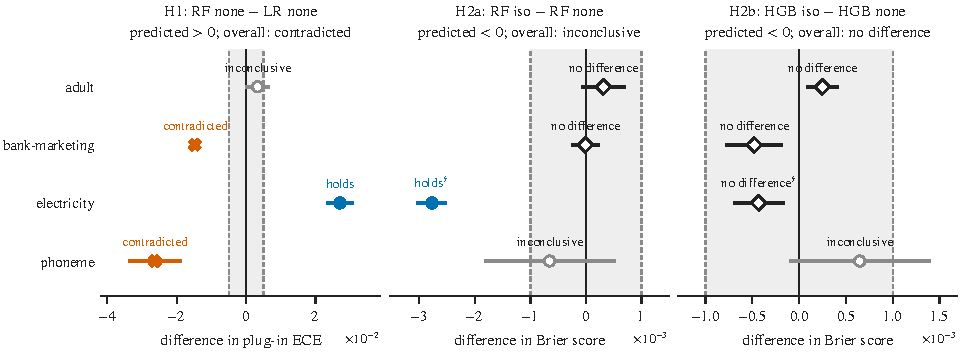
\includegraphics[width=\textwidth]{figures/fig_intervals.pdf}
\caption{The intervals of Table~\ref{tab:decision} as a forest plot, one panel per
hypothesis. Each row is a dataset: the marker is the mean of the 10 paired per-seed
differences and the line its 95\% paired $t(9)$ interval. The solid vertical line is zero;
the dashed lines and gray band mark $\pm$ the margin (0.005 ECE for H1, 0.001 Brier for H2a
and H2b). Markers give the category: filled circle \cat{holds}, cross \cat{contradicted},
open diamond \cat{no difference}, open gray circle \cat{inconclusive}. Panel titles give the
overall verdict. The x-axes differ between panels and are scaled by the factor printed at
their right end. A dagger on \el's category label marks the hypotheses whose overall verdict
would change if \el's category changed (H2a and H2b); H1's does not depend on \el.}
\label{fig:intervals}
\end{figure}

\subsection{H1: uncalibrated random forest against logistic regression (plug-in ECE)}
\label{sec:h1}

\textbf{H1 is \cat{contradicted} overall.} The difference RF minus LR in plug-in ECE was
negative, against the prediction, with intervals wholly below zero on \bm{}
(\md{\HOneBankMean}{\HOneBankLo}{\HOneBankHi}) and \ph{}
(\md{\HOnePhonemeMean}{\HOnePhonemeLo}{\HOnePhonemeHi}). It held on \el{}
(\md{\HOneElecMean}{\HOneElecLo}{\HOneElecHi}), and on \ad{} the interval
(\md{\HOneAdultMean}{\HOneAdultLo}{\HOneAdultHi}) crosses zero and extends beyond the margin,
so there is no detectable difference (inconclusive). Two contradictions suffice for the
overall \cat{contradicted}, so \textbf{this verdict does not depend on \el}: it would be the
same whatever \el's category.

What the contradiction shows is limited. It comes from default LR's own miscalibration on two
datasets, not from RF being well calibrated. LR's plug-in ECE was $\BankLrNoneEce$ on \bm{}
and $\PhonemeLrNoneEce$ on \ph, against $\AdultLrNoneEce$ on \ad{} and $\ElecLrNoneEce$ on
\el{} (Table~\ref{tab:levels}). On \ph{} the linear model also discriminated much worse than
the trees (AUC $\PhonemeLrNoneAuc$ against RF's $\PhonemeRfNoneAuc$), and Platt scaling left
its ECE at $\PhonemeLrPlattEce$. The uncalibrated RF still had ECE $\BankRfNoneEce$ on \bm{}
and $\PhonemeRfNoneEce$ on \ph. The two arms are also scored on different numbers of bins:
RF's outputs tie at multiples of 0.01, so uncalibrated RF used $\AdultRfNoneEceBins$,
$\BankRfNoneEceBins$, $\ElecRfNoneEceBins$ and $\PhonemeRfNoneEceBins$ non-empty bins on
average on \ad, \bm, \el{} and \ph, against $\AdultLrNoneEceBins$, $\BankLrNoneEceBins$,
$\ElecLrNoneEceBins$ and $\PhonemeLrNoneEceBins$ for LR. ECE values on different numbers of bins
are not on an identical footing, which is part of why we read H1 as a statement about the
estimator.

\paragraph{Debiased ECE (descriptive).} Recomputed on the debiased ECE, the differences have
the same sign on every dataset (Table~\ref{tab:sens}, Panel~A): \md{\HOneDbBankMean}{\HOneDbBankLo}{\HOneDbBankHi}
on \bm, \md{\HOneDbPhonemeMean}{\HOneDbPhonemeLo}{\HOneDbPhonemeHi} on \ph,
\md{\HOneDbElecMean}{\HOneDbElecLo}{\HOneDbElecHi} on \el, and on \ad{}
\md{\HOneDbAdultMean}{\HOneDbAdultLo}{\HOneDbAdultHi}, an interval that lies wholly above zero.
Under the same rule this would also read \cat{contradicted} overall. This is descriptive and
does not change H1. Because the debiased estimator keeps about 0.6 of any floor difference
with its sign, its agreement with the plug-in result is not confirmation, and \ad's move from
inconclusive to holds on this estimator is not evidence for H1 on \ad. On \bm{} and \ph,
LR's debiased ECE ($\BankLrNoneEceDb$ and $\PhonemeLrNoneEceDb$) stayed close to its plug-in
value, as expected for a clearly miscalibrated model.

\paragraph{Proper scores (descriptive).} On the Brier score, uncalibrated RF minus LR was
\md{\BankRfMinusLrBrierMean}{\BankRfMinusLrBrierLo}{\BankRfMinusLrBrierHi} on \bm,
\md{\ElecRfMinusLrBrierMean}{\ElecRfMinusLrBrierLo}{\ElecRfMinusLrBrierHi} on \el{} and
\md{\PhonemeRfMinusLrBrierMean}{\PhonemeRfMinusLrBrierLo}{\PhonemeRfMinusLrBrierHi} on \ph,
so RF had the lower Brier score there, while on \ad{} RF's was higher,
\md{\AdultRfMinusLrBrierMean}{\AdultRfMinusLrBrierLo}{\AdultRfMinusLrBrierHi}. Log-loss shows
the same pattern (\ad{} \md{\AdultRfMinusLrLoglossMean}{\AdultRfMinusLrLoglossLo}{\AdultRfMinusLrLoglossHi};
\bm{} \md{\BankRfMinusLrLoglossMean}{\BankRfMinusLrLoglossLo}{\BankRfMinusLrLoglossHi};
\el{} \md{\ElecRfMinusLrLoglossMean}{\ElecRfMinusLrLoglossLo}{\ElecRfMinusLrLoglossHi};
\ph{} \md{\PhonemeRfMinusLrLoglossMean}{\PhonemeRfMinusLrLoglossLo}{\PhonemeRfMinusLrLoglossHi}).
These proper scores also reward discrimination, so they do not bear on H1 directly; on three
of four datasets they point the same way as the observation of \citet{fonseca2017} that
uncalibrated random forests often beat LR on the Brier score.

\subsection{H2a: isotonic recalibration of random forests (Brier score)}
\label{sec:h2a}

\textbf{H2a is \cat{inconclusive} overall, and this verdict depends on \el.} Isotonic
regression lowered RF's Brier score beyond the 0.001 margin only on \el{}
(\md{\HTwoAElecMean}{\HTwoAElecLo}{\HTwoAElecHi}, \cat{holds}). On \ad{}
(\md{\HTwoAAdultMean}{\HTwoAAdultLo}{\HTwoAAdultHi}) and \bm{}
(\md{\HTwoABankMean}{\HTwoABankLo}{\HTwoABankHi}) the whole interval lies inside $\pm0.001$
(\cat{no difference}). The \bm{} mean prints as $\HTwoABankMean$: the mean change is
negative, a fall in the Brier score, but so small that it rounds to zero at four decimals; it
is not exactly zero, and its interval is well inside the margin on both
sides. On \ph{} (\md{\HTwoAPhonemeMean}{\HTwoAPhonemeLo}{\HTwoAPhonemeHi}) the interval
crosses both zero and $-0.001$, so there is no detectable difference (inconclusive). With one
\cat{holds}, two \cat{no difference} and one inconclusive, the k-of-4 rule gives
\cat{inconclusive}.

\el's \cat{holds} is what keeps H2a from \cat{no difference}: had \el{} been \cat{no
difference}, H2a would be \cat{no difference} on three of four datasets; had it been
contradicted or inconclusive, or been dropped, H2a would remain \cat{inconclusive}. Since
\el's random splits may leak information across neighbouring half-hours
(Section~\ref{sec:elec}), the basis of H2a's verdict is open. H2a is not supported on these
samples.

\paragraph{Descriptive.} The isotonic map did not lower RF's discrimination by much: isotonic
minus Platt AUC (Platt preserves the ranking) was $\AdultRfIsoMinusPlattAuc$,
$\BankRfIsoMinusPlattAuc$, $\ElecRfIsoMinusPlattAuc$ and $\PhonemeRfIsoMinusPlattAuc$ on
\ad, \bm, \el{} and \ph. RF's log-loss moved from $\AdultRfNoneLogloss$ to
$\AdultRfIsoLogloss$ on \ad, $\BankRfNoneLogloss$ to $\BankRfIsoLogloss$ on \bm,
$\ElecRfNoneLogloss$ to $\ElecRfIsoLogloss$ on \el{} and $\PhonemeRfNoneLogloss$ to
$\PhonemeRfIsoLogloss$ on \ph{} (none to isotonic). Uncalibrated RF outputs many exact zeros:
on average $\AdultRfNoneClipLow$, $\BankRfNoneClipLow$, $\ElecRfNoneClipLow$ and
$\PhonemeRfNoneClipLow$ of its test predictions per seed fell below $10^{-6}$ on the four
datasets, so its log-loss depends on the clipping constant. In the planned sensitivity that
clips at machine epsilon instead of $10^{-6}$, uncalibrated RF's log-loss rose to
$\AdultRfNoneLoglossMach$ ($\AdultRfNoneLoglossMachSd$), $\BankRfNoneLoglossMach$
($\BankRfNoneLoglossMachSd$), $\ElecRfNoneLoglossMach$ ($\ElecRfNoneLoglossMachSd$) and
$\PhonemeRfNoneLoglossMach$ ($\PhonemeRfNoneLoglossMachSd$) on \ad, \bm, \el{} and \ph{}
(mean (SD) over seeds), and RF with isotonic regression to $\AdultRfIsoLoglossMach$,
$\BankRfIsoLoglossMach$, $\ElecRfIsoLoglossMach$ and $\PhonemeRfIsoLoglossMach$. At this
clipping constant isotonic's log-loss advantage over no recalibration is larger on \ad, and on
\ph{} the two are equal at three decimals, as they are at $10^{-6}$; the log-loss comparison is
descriptive at either constant. Across all 360 cells,
$\ClipLowTotal$ predictions fell below $10^{-6}$ and $\ClipHighTotal$ above $1-10^{-6}$. The
ECE of RF was lower with isotonic than without on each dataset in Table~\ref{tab:levels} (for
example $\ElecRfNoneEce$ to $\ElecRfIsoEce$ on \el), but isotonic outputs tie and were scored
on fewer bins ($\AdultRfIsoEceBins$, $\BankRfIsoEceBins$, $\ElecRfIsoEceBins$ and
$\PhonemeRfIsoEceBins$ on average), and fewer, larger bins lower the plug-in noise floor, so
these ECE reductions partly reflect bin count. No verdict uses isotonic ECE.

\subsection{H2b: isotonic recalibration of gradient boosting (Brier score)}
\label{sec:h2b}

\textbf{H2b is \cat{no difference} overall, and this verdict depends on \el.} On \ad{}
(\md{\HTwoBAdultMean}{\HTwoBAdultLo}{\HTwoBAdultHi}), \bm{}
(\md{\HTwoBBankMean}{\HTwoBBankLo}{\HTwoBBankHi}) and \el{}
(\md{\HTwoBElecMean}{\HTwoBElecLo}{\HTwoBElecHi}) the whole interval lies inside $\pm0.001$,
so the rule's first category, \cat{no difference}, applies. On \ph{}
(\md{\HTwoBPhonemeMean}{\HTwoBPhonemeLo}{\HTwoBPhonemeHi}) the interval crosses zero and the
upper margin, so there is no detectable difference (inconclusive). Three \cat{no difference}
and none holding or contradicted give \cat{no difference} overall.

\cat{No difference} here means that each change was smaller than the 0.001 margin, not that
isotonic had no effect. \ad's interval lies wholly above zero (isotonic raised HGB's Brier
score, by less than the margin), and \bm's and \el's lie wholly below zero (it lowered it, by
less than the margin). The verdict needs \el{} as one of its three \cat{no difference}
datasets; with any other category on \el{} it would be \cat{inconclusive}. Isotonic minus
Platt AUC for HGB was $\AdultHgbIsoMinusPlattAuc$, $\BankHgbIsoMinusPlattAuc$,
$\ElecHgbIsoMinusPlattAuc$ and $\PhonemeHgbIsoMinusPlattAuc$ on the four datasets, and HGB's
log-loss went from $\AdultHgbNoneLogloss$ to $\AdultHgbIsoLogloss$ on \ad,
$\BankHgbNoneLogloss$ to $\BankHgbIsoLogloss$ on \bm, $\ElecHgbNoneLogloss$ to
$\ElecHgbIsoLogloss$ on \el{} and $\PhonemeHgbNoneLogloss$ to $\PhonemeHgbIsoLogloss$ on \ph{}
(descriptive). Clipped at machine epsilon, where isotonic's exact zeros and ones weigh more,
HGB's log-loss went from $\AdultHgbNoneLoglossMach$ to $\AdultHgbIsoLoglossMach$,
$\BankHgbNoneLoglossMach$ to $\BankHgbIsoLoglossMach$, $\ElecHgbNoneLoglossMach$ to
$\ElecHgbIsoLoglossMach$ and $\PhonemeHgbNoneLoglossMach$ to $\PhonemeHgbIsoLoglossMach$.

\subsection{Calibration levels and Platt scaling (descriptive)}
\label{sec:levels}

Figure~\ref{fig:reliability} shows reliability diagrams for every dataset and model, without
recalibration and with isotonic regression, binned by the ECE's own rule; the box in each
panel gives the plug-in ECE as mean (SD) over seeds and the mean number of non-empty bins.
Table~\ref{tab:levels} gives every level. Default HGB had the lowest Brier score on \ad{}
($\AdultHgbNoneBrier$, against $\AdultLrNoneBrier$ for LR and $\AdultRfNoneBrier$ for RF), and
RF and HGB had far lower Brier scores than LR on \el{} and \ph.

Platt scaling, fitted on the logit, changed little except for the tree models on \el. Platt minus none on the Brier score was
\md{\AdultLrPlattMinusNoneBrierMean}{\AdultLrPlattMinusNoneBrierLo}{\AdultLrPlattMinusNoneBrierHi},
\md{\BankLrPlattMinusNoneBrierMean}{\BankLrPlattMinusNoneBrierLo}{\BankLrPlattMinusNoneBrierHi},
\md{\ElecLrPlattMinusNoneBrierMean}{\ElecLrPlattMinusNoneBrierLo}{\ElecLrPlattMinusNoneBrierHi}
and
\md{\PhonemeLrPlattMinusNoneBrierMean}{\PhonemeLrPlattMinusNoneBrierLo}{\PhonemeLrPlattMinusNoneBrierHi}
for LR on \ad, \bm, \el{} and \ph; for RF it was largest on \el{}
(\md{\ElecRfPlattMinusNoneBrierMean}{\ElecRfPlattMinusNoneBrierLo}{\ElecRfPlattMinusNoneBrierHi}),
the same size as isotonic's change there, which is H2a's one \cat{holds}; for HGB it was largest on \el{}
(\md{\ElecHgbPlattMinusNoneBrierMean}{\ElecHgbPlattMinusNoneBrierLo}{\ElecHgbPlattMinusNoneBrierHi}).
These intervals are descriptive; no margin or rule applies to them. Where LR was
miscalibrated, isotonic regression changed more than Platt scaling did: on \bm{} LR's ECE went
from $\BankLrNoneEce$ (none) and $\BankLrPlattEce$ (Platt) to $\BankLrIsoEce$ (isotonic) and its
Brier score from $\BankLrNoneBrier$ to $\BankLrIsoBrier$; on \ph{} its ECE went from
$\PhonemeLrNoneEce$ and $\PhonemeLrPlattEce$ to $\PhonemeLrIsoEce$ and its Brier score from
$\PhonemeLrNoneBrier$ to $\PhonemeLrIsoBrier$. The isotonic ECE values were again scored on
fewer bins ($\BankLrIsoEceBins$ and $\PhonemeLrIsoEceBins$, against $\BankLrNoneEceBins$ and
$\PhonemeLrNoneEceBins$ without recalibration). On \ph{} isotonic
regression raised LR's AUC slightly (isotonic minus Platt $\PhonemeLrIsoMinusPlattAuc$).

\begin{figure}[!htbp]
\centering
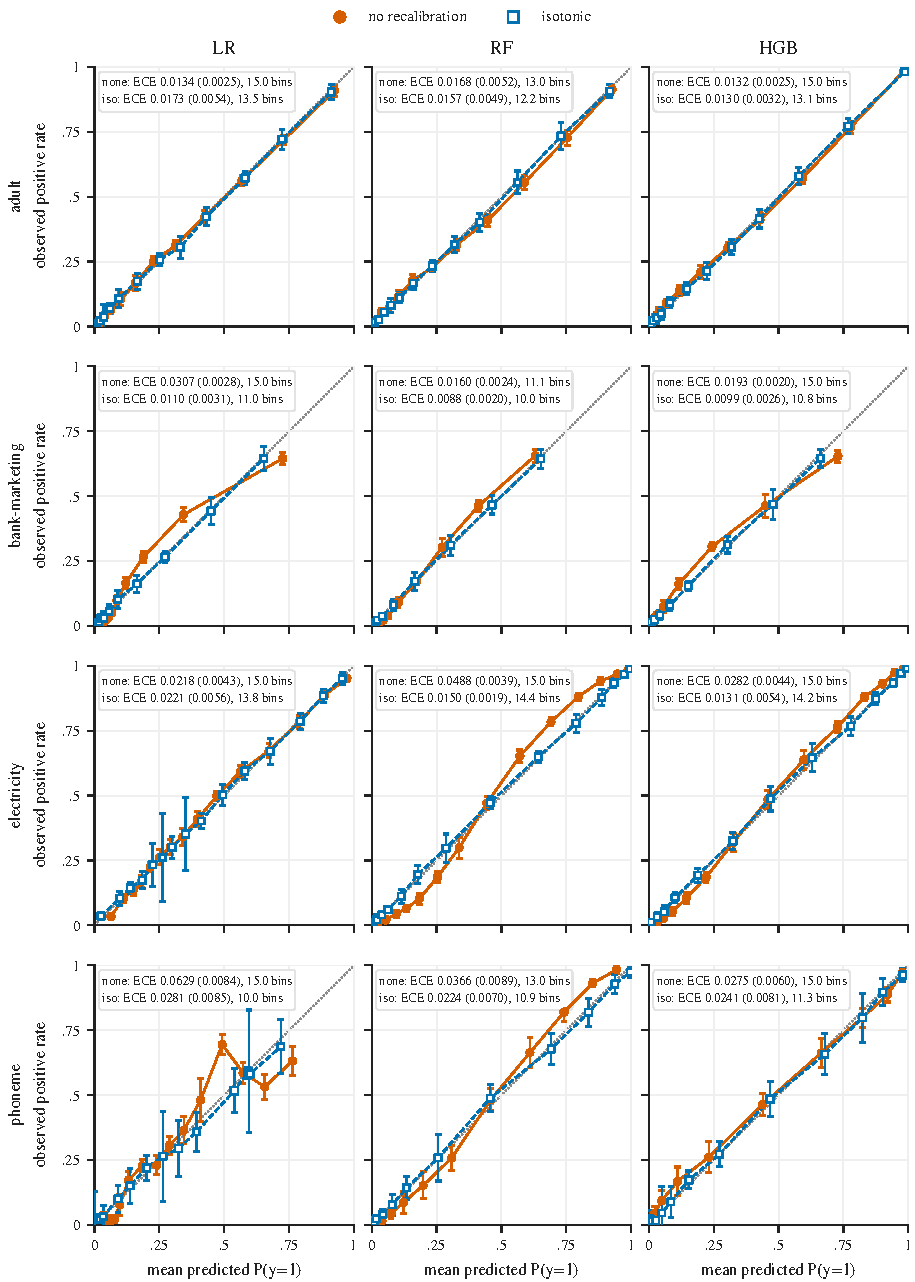
\includegraphics[width=0.70\textwidth]{figures/fig_reliability.pdf}
\caption{Reliability diagrams of LR, RF and HGB (columns) on each dataset (rows), without
recalibration (filled circles, solid line) and with isotonic regression fitted on the
calibration split (open squares, dashed line). Test-split predictions are pooled over the 10
seeds (50,000 rows per curve on \ad, \bm{} and \el; 13,510 on \ph) and grouped by the ECE's
rule: 15 equal-mass bins on $P(y=1)$, tied predictions never split. Each point is one
non-empty pooled bin at its mean prediction and observed positive rate; marker area is
proportional to the bin's share of rows. Error bars are $\pm1$ SD across seeds of the positive
rate in the bin (a seed spread). The dotted diagonal is perfect calibration. The box in each panel
gives, per calibrator, the plug-in ECE as mean (SD) over the per-seed values and the mean
number of non-empty bins per seed, as in Table~\ref{tab:levels}; pooling over seeds breaks
most of isotonic's ties, so isotonic curves show more pooled points than the per-seed bin
count. The \bm{} panels crowd below 0.2 because 11.7\% of its rows are positive. \el{} uses
random splits of a time series (Section~\ref{sec:elec}); the curves describe these samples
only.}
\label{fig:reliability}
\end{figure}

\subsection{Calibration-set size (sensitivity b)}
\label{sec:ncal}

\ph's calibration split has 1,351 rows, against 5,000 elsewhere. Refitting isotonic regression
on 1,351 calibration rows on the other three datasets (Table~\ref{tab:sens}, Panel~B) gives,
for H2a, \cat{contradicted} on \ad{}
(\md{\HTwoANcalAdultMean}{\HTwoANcalAdultLo}{\HTwoANcalAdultHi}) and on \bm{}
(\md{\HTwoANcalBankMean}{\HTwoANcalBankLo}{\HTwoANcalBankHi}), and \cat{holds} on \el{}
(\md{\HTwoANcalElecMean}{\HTwoANcalElecLo}{\HTwoANcalElecHi}). Both contradictions rest on mean
Brier rises below 0.001 whose intervals cross the margin only at their upper ends. For H2b it
gives \cat{contradicted} on \ad{} (\md{\HTwoBNcalAdultMean}{\HTwoBNcalAdultLo}{\HTwoBNcalAdultHi})
and \cat{no difference} on \bm{} and \el. So with the smaller calibration split, isotonic
regression tended to raise the Brier score slightly on \ad{} and \bm, which is consistent
with, but does not show, an effect of calibration-set size in this range. The comparison equalises calibration size only,
so it does not show why \ph's own results differ, and none of this changes a verdict.

\subsection{Electricity under a chronological split (sensitivity c)}
\label{sec:elec}

Under the chronological split, H1 was inconclusive on \el{}
(\md{\HOneTimeElecMean}{\HOneTimeElecLo}{\HOneTimeElecHi}), H2a was contradicted
(\md{\HTwoATimeElecMean}{\HTwoATimeElecLo}{\HTwoATimeElecHi}) and H2b held
(\md{\HTwoBTimeElecMean}{\HTwoBTimeElecLo}{\HTwoBTimeElecHi}). These categories cannot be read
as \el's results without leakage, because the split changes much more than leakage
(Table~\ref{tab:electime}). All three uncalibrated models were badly miscalibrated on the
test quarter, with ECE $\ElecTimeLrNoneEce$ (LR), $\ElecTimeRfNoneEce$ (RF) and
$\ElecTimeHgbNoneEce$ (HGB), against $\ElecLrNoneEce$, $\ElecRfNoneEce$ and $\ElecHgbNoneEce$
under random splits; and recalibration fitted on the calibration quarter could make the test
quarter worse: LR's Brier score was $\ElecTimeLrNoneBrier$ with no recalibration,
$\ElecTimeLrPlattBrier$ with Platt and $\ElecTimeLrIsoBrier$ with isotonic. The calibration and
test quarters thus differ in distribution. The split also puts every Victoria fill-value row
into training ($\TimeVicfillTrainMin$ to $\TimeVicfillTrainMax$ per seed, against
$\TimeVicfillCalMax$ in calibration and $\TimeVicfillTestMax$ in test; under random splits the
seed means were $\MainVicfillTrainMean$, $\MainVicfillCalMean$ and $\MainVicfillTestMean$), and
places test dates beyond most of the training range. The run therefore measures drift between
periods, mixed with the fill regime. It does not show whether random-split leakage drives the
main \el{} results, and the H2b result under this split is not evidence that isotonic
regression helps gradient boosting under drift. \textbf{Whether leakage drives \el's
results, and with it the basis of the H2a and H2b verdicts, remains open.}

\begin{table}[!htbp]
\centering
\small
% Generated by code/tab_sensitivity.py from logged runs. Do not edit by hand; rerun the script.
% Needs \usepackage{booktabs} and % Generated by `crew.py numbers` from claims.jsonl. Do not edit by hand.
% Each macro is a number taken from a logged run; see claims.jsonl.
\newcommand{\HOneAdultMean}{0.0033}  % r-h1-adult-mean
\newcommand{\HOneAdultLo}{-0.0001}  % r-h1-adult-lo
\newcommand{\HOneAdultHi}{0.0068}  % r-h1-adult-hi
\newcommand{\HOneAdultCat}{3}  % r-h1-adult-cat
\newcommand{\HOneBankMean}{-0.0147}  % r-h1-bank-marketing-mean
\newcommand{\HOneBankLo}{-0.0161}  % r-h1-bank-marketing-lo
\newcommand{\HOneBankHi}{-0.0134}  % r-h1-bank-marketing-hi
\newcommand{\HOneBankCat}{2}  % r-h1-bank-marketing-cat
\newcommand{\HOneElecMean}{0.0270}  % r-h1-electricity-mean
\newcommand{\HOneElecLo}{0.0232}  % r-h1-electricity-lo
\newcommand{\HOneElecHi}{0.0308}  % r-h1-electricity-hi
\newcommand{\HOneElecCat}{1}  % r-h1-electricity-cat
\newcommand{\HOnePhonemeMean}{-0.0263}  % r-h1-phoneme-mean
\newcommand{\HOnePhonemeLo}{-0.0339}  % r-h1-phoneme-lo
\newcommand{\HOnePhonemeHi}{-0.0187}  % r-h1-phoneme-hi
\newcommand{\HOnePhonemeCat}{2}  % r-h1-phoneme-cat
\newcommand{\HOneOverallCode}{2}  % r-h1-overall
\newcommand{\HTwoAAdultMean}{0.0003}  % r-h2a-adult-mean
\newcommand{\HTwoAAdultLo}{-0.0001}  % r-h2a-adult-lo
\newcommand{\HTwoAAdultHi}{0.0007}  % r-h2a-adult-hi
\newcommand{\HTwoAAdultCat}{0}  % r-h2a-adult-cat
\newcommand{\HTwoABankMean}{-0.0000}  % r-h2a-bank-marketing-mean
\newcommand{\HTwoABankLo}{-0.0003}  % r-h2a-bank-marketing-lo
\newcommand{\HTwoABankHi}{0.0002}  % r-h2a-bank-marketing-hi
\newcommand{\HTwoABankCat}{0}  % r-h2a-bank-marketing-cat
\newcommand{\HTwoAElecMean}{-0.0028}  % r-h2a-electricity-mean
\newcommand{\HTwoAElecLo}{-0.0030}  % r-h2a-electricity-lo
\newcommand{\HTwoAElecHi}{-0.0025}  % r-h2a-electricity-hi
\newcommand{\HTwoAElecCat}{1}  % r-h2a-electricity-cat
\newcommand{\HTwoAPhonemeMean}{-0.0007}  % r-h2a-phoneme-mean
\newcommand{\HTwoAPhonemeLo}{-0.0018}  % r-h2a-phoneme-lo
\newcommand{\HTwoAPhonemeHi}{0.0005}  % r-h2a-phoneme-hi
\newcommand{\HTwoAPhonemeCat}{3}  % r-h2a-phoneme-cat
\newcommand{\HTwoAOverallCode}{3}  % r-h2a-overall
\newcommand{\HTwoBAdultMean}{0.0002}  % r-h2b-adult-mean
\newcommand{\HTwoBAdultLo}{0.0001}  % r-h2b-adult-lo
\newcommand{\HTwoBAdultHi}{0.0004}  % r-h2b-adult-hi
\newcommand{\HTwoBAdultCat}{0}  % r-h2b-adult-cat
\newcommand{\HTwoBBankMean}{-0.0005}  % r-h2b-bank-marketing-mean
\newcommand{\HTwoBBankLo}{-0.0008}  % r-h2b-bank-marketing-lo
\newcommand{\HTwoBBankHi}{-0.0002}  % r-h2b-bank-marketing-hi
\newcommand{\HTwoBBankCat}{0}  % r-h2b-bank-marketing-cat
\newcommand{\HTwoBElecMean}{-0.0004}  % r-h2b-electricity-mean
\newcommand{\HTwoBElecLo}{-0.0007}  % r-h2b-electricity-lo
\newcommand{\HTwoBElecHi}{-0.0002}  % r-h2b-electricity-hi
\newcommand{\HTwoBElecCat}{0}  % r-h2b-electricity-cat
\newcommand{\HTwoBPhonemeMean}{0.0006}  % r-h2b-phoneme-mean
\newcommand{\HTwoBPhonemeLo}{-0.0001}  % r-h2b-phoneme-lo
\newcommand{\HTwoBPhonemeHi}{0.0014}  % r-h2b-phoneme-hi
\newcommand{\HTwoBPhonemeCat}{3}  % r-h2b-phoneme-cat
\newcommand{\HTwoBOverallCode}{0}  % r-h2b-overall
\newcommand{\HOneDbAdultMean}{0.0042}  % r-h1db-adult-mean
\newcommand{\HOneDbAdultLo}{0.0002}  % r-h1db-adult-lo
\newcommand{\HOneDbAdultHi}{0.0082}  % r-h1db-adult-hi
\newcommand{\HOneDbAdultCat}{1}  % r-h1db-adult-cat
\newcommand{\HOneDbBankMean}{-0.0160}  % r-h1db-bank-marketing-mean
\newcommand{\HOneDbBankLo}{-0.0173}  % r-h1db-bank-marketing-lo
\newcommand{\HOneDbBankHi}{-0.0147}  % r-h1db-bank-marketing-hi
\newcommand{\HOneDbBankCat}{2}  % r-h1db-bank-marketing-cat
\newcommand{\HOneDbElecMean}{0.0322}  % r-h1db-electricity-mean
\newcommand{\HOneDbElecLo}{0.0275}  % r-h1db-electricity-lo
\newcommand{\HOneDbElecHi}{0.0369}  % r-h1db-electricity-hi
\newcommand{\HOneDbElecCat}{1}  % r-h1db-electricity-cat
\newcommand{\HOneDbPhonemeMean}{-0.0235}  % r-h1db-phoneme-mean
\newcommand{\HOneDbPhonemeLo}{-0.0329}  % r-h1db-phoneme-lo
\newcommand{\HOneDbPhonemeHi}{-0.0142}  % r-h1db-phoneme-hi
\newcommand{\HOneDbPhonemeCat}{2}  % r-h1db-phoneme-cat
\newcommand{\HOneDbOverallCode}{2}  % r-h1db-overall
\newcommand{\HTwoANcalAdultMean}{0.0009}  % r-h2a_ncal-adult-mean
\newcommand{\HTwoANcalAdultLo}{0.0005}  % r-h2a_ncal-adult-lo
\newcommand{\HTwoANcalAdultHi}{0.0012}  % r-h2a_ncal-adult-hi
\newcommand{\HTwoANcalAdultCat}{2}  % r-h2a_ncal-adult-cat
\newcommand{\HTwoANcalBankMean}{0.0008}  % r-h2a_ncal-bank-marketing-mean
\newcommand{\HTwoANcalBankLo}{0.0006}  % r-h2a_ncal-bank-marketing-lo
\newcommand{\HTwoANcalBankHi}{0.0011}  % r-h2a_ncal-bank-marketing-hi
\newcommand{\HTwoANcalBankCat}{2}  % r-h2a_ncal-bank-marketing-cat
\newcommand{\HTwoANcalElecMean}{-0.0022}  % r-h2a_ncal-electricity-mean
\newcommand{\HTwoANcalElecLo}{-0.0026}  % r-h2a_ncal-electricity-lo
\newcommand{\HTwoANcalElecHi}{-0.0018}  % r-h2a_ncal-electricity-hi
\newcommand{\HTwoANcalElecCat}{1}  % r-h2a_ncal-electricity-cat
\newcommand{\HTwoANcalOverallCode}{2}  % r-h2a-ncal-overall
\newcommand{\HTwoBNcalAdultMean}{0.0010}  % r-h2b_ncal-adult-mean
\newcommand{\HTwoBNcalAdultLo}{0.0007}  % r-h2b_ncal-adult-lo
\newcommand{\HTwoBNcalAdultHi}{0.0013}  % r-h2b_ncal-adult-hi
\newcommand{\HTwoBNcalAdultCat}{2}  % r-h2b_ncal-adult-cat
\newcommand{\HTwoBNcalBankMean}{0.0001}  % r-h2b_ncal-bank-marketing-mean
\newcommand{\HTwoBNcalBankLo}{-0.0004}  % r-h2b_ncal-bank-marketing-lo
\newcommand{\HTwoBNcalBankHi}{0.0006}  % r-h2b_ncal-bank-marketing-hi
\newcommand{\HTwoBNcalBankCat}{0}  % r-h2b_ncal-bank-marketing-cat
\newcommand{\HTwoBNcalElecMean}{0.0001}  % r-h2b_ncal-electricity-mean
\newcommand{\HTwoBNcalElecLo}{-0.0002}  % r-h2b_ncal-electricity-lo
\newcommand{\HTwoBNcalElecHi}{0.0004}  % r-h2b_ncal-electricity-hi
\newcommand{\HTwoBNcalElecCat}{0}  % r-h2b_ncal-electricity-cat
\newcommand{\HTwoBNcalOverallCode}{3}  % r-h2b-ncal-overall
\newcommand{\HOneTimeElecMean}{0.0008}  % r-h1_time-electricity-mean
\newcommand{\HOneTimeElecLo}{-0.0100}  % r-h1_time-electricity-lo
\newcommand{\HOneTimeElecHi}{0.0116}  % r-h1_time-electricity-hi
\newcommand{\HOneTimeElecCat}{3}  % r-h1_time-electricity-cat
\newcommand{\HTwoATimeElecMean}{0.0265}  % r-h2a_time-electricity-mean
\newcommand{\HTwoATimeElecLo}{0.0209}  % r-h2a_time-electricity-lo
\newcommand{\HTwoATimeElecHi}{0.0322}  % r-h2a_time-electricity-hi
\newcommand{\HTwoATimeElecCat}{2}  % r-h2a_time-electricity-cat
\newcommand{\HTwoBTimeElecMean}{-0.0782}  % r-h2b_time-electricity-mean
\newcommand{\HTwoBTimeElecLo}{-0.1013}  % r-h2b_time-electricity-lo
\newcommand{\HTwoBTimeElecHi}{-0.0551}  % r-h2b_time-electricity-hi
\newcommand{\HTwoBTimeElecCat}{1}  % r-h2b_time-electricity-cat
\newcommand{\ElecTimeLrNoneEce}{0.1677}  % r-time-lr-none-ece-mean
\newcommand{\ElecTimeLrNoneEceSd}{0.0057}  % r-time-lr-none-ece-sd
\newcommand{\ElecTimeLrNoneBrier}{0.2018}  % r-time-lr-none-brier-mean
\newcommand{\ElecTimeLrNoneBrierSd}{0.0031}  % r-time-lr-none-brier-sd
\newcommand{\ElecTimeLrNoneAuc}{0.841}  % r-time-lr-none-auc-mean
\newcommand{\ElecTimeLrNoneAucSd}{0.0035}  % r-time-lr-none-auc-sd
\newcommand{\ElecTimeLrPlattEce}{0.2785}  % r-time-lr-platt-ece-mean
\newcommand{\ElecTimeLrPlattEceSd}{0.0052}  % r-time-lr-platt-ece-sd
\newcommand{\ElecTimeLrPlattBrier}{0.2509}  % r-time-lr-platt-brier-mean
\newcommand{\ElecTimeLrPlattBrierSd}{0.0026}  % r-time-lr-platt-brier-sd
\newcommand{\ElecTimeLrPlattAuc}{0.841}  % r-time-lr-platt-auc-mean
\newcommand{\ElecTimeLrPlattAucSd}{0.0035}  % r-time-lr-platt-auc-sd
\newcommand{\ElecTimeLrIsoEce}{0.2621}  % r-time-lr-isotonic-ece-mean
\newcommand{\ElecTimeLrIsoEceSd}{0.0074}  % r-time-lr-isotonic-ece-sd
\newcommand{\ElecTimeLrIsoBrier}{0.2531}  % r-time-lr-isotonic-brier-mean
\newcommand{\ElecTimeLrIsoBrierSd}{0.0030}  % r-time-lr-isotonic-brier-sd
\newcommand{\ElecTimeLrIsoAuc}{0.817}  % r-time-lr-isotonic-auc-mean
\newcommand{\ElecTimeLrIsoAucSd}{0.0110}  % r-time-lr-isotonic-auc-sd
\newcommand{\ElecTimeRfNoneEce}{0.1685}  % r-time-rf-none-ece-mean
\newcommand{\ElecTimeRfNoneEceSd}{0.0156}  % r-time-rf-none-ece-sd
\newcommand{\ElecTimeRfNoneBrier}{0.1971}  % r-time-rf-none-brier-mean
\newcommand{\ElecTimeRfNoneBrierSd}{0.0046}  % r-time-rf-none-brier-sd
\newcommand{\ElecTimeRfNoneAuc}{0.828}  % r-time-rf-none-auc-mean
\newcommand{\ElecTimeRfNoneAucSd}{0.0046}  % r-time-rf-none-auc-sd
\newcommand{\ElecTimeRfPlattEce}{0.1975}  % r-time-rf-platt-ece-mean
\newcommand{\ElecTimeRfPlattEceSd}{0.0157}  % r-time-rf-platt-ece-sd
\newcommand{\ElecTimeRfPlattBrier}{0.2091}  % r-time-rf-platt-brier-mean
\newcommand{\ElecTimeRfPlattBrierSd}{0.0072}  % r-time-rf-platt-brier-sd
\newcommand{\ElecTimeRfPlattAuc}{0.828}  % r-time-rf-platt-auc-mean
\newcommand{\ElecTimeRfPlattAucSd}{0.0046}  % r-time-rf-platt-auc-sd
\newcommand{\ElecTimeRfIsoEce}{0.2050}  % r-time-rf-isotonic-ece-mean
\newcommand{\ElecTimeRfIsoEceSd}{0.0112}  % r-time-rf-isotonic-ece-sd
\newcommand{\ElecTimeRfIsoBrier}{0.2236}  % r-time-rf-isotonic-brier-mean
\newcommand{\ElecTimeRfIsoBrierSd}{0.0069}  % r-time-rf-isotonic-brier-sd
\newcommand{\ElecTimeRfIsoAuc}{0.817}  % r-time-rf-isotonic-auc-mean
\newcommand{\ElecTimeRfIsoAucSd}{0.0067}  % r-time-rf-isotonic-auc-sd
\newcommand{\ElecTimeHgbNoneEce}{0.3339}  % r-time-hgb-none-ece-mean
\newcommand{\ElecTimeHgbNoneEceSd}{0.0270}  % r-time-hgb-none-ece-sd
\newcommand{\ElecTimeHgbNoneBrier}{0.3271}  % r-time-hgb-none-brier-mean
\newcommand{\ElecTimeHgbNoneBrierSd}{0.0274}  % r-time-hgb-none-brier-sd
\newcommand{\ElecTimeHgbNoneAuc}{0.841}  % r-time-hgb-none-auc-mean
\newcommand{\ElecTimeHgbNoneAucSd}{0.0085}  % r-time-hgb-none-auc-sd
\newcommand{\ElecTimeHgbPlattEce}{0.2456}  % r-time-hgb-platt-ece-mean
\newcommand{\ElecTimeHgbPlattEceSd}{0.0180}  % r-time-hgb-platt-ece-sd
\newcommand{\ElecTimeHgbPlattBrier}{0.2453}  % r-time-hgb-platt-brier-mean
\newcommand{\ElecTimeHgbPlattBrierSd}{0.0148}  % r-time-hgb-platt-brier-sd
\newcommand{\ElecTimeHgbPlattAuc}{0.841}  % r-time-hgb-platt-auc-mean
\newcommand{\ElecTimeHgbPlattAucSd}{0.0085}  % r-time-hgb-platt-auc-sd
\newcommand{\ElecTimeHgbIsoEce}{0.2406}  % r-time-hgb-isotonic-ece-mean
\newcommand{\ElecTimeHgbIsoEceSd}{0.0119}  % r-time-hgb-isotonic-ece-sd
\newcommand{\ElecTimeHgbIsoBrier}{0.2489}  % r-time-hgb-isotonic-brier-mean
\newcommand{\ElecTimeHgbIsoBrierSd}{0.0105}  % r-time-hgb-isotonic-brier-sd
\newcommand{\ElecTimeHgbIsoAuc}{0.813}  % r-time-hgb-isotonic-auc-mean
\newcommand{\ElecTimeHgbIsoAucSd}{0.0140}  % r-time-hgb-isotonic-auc-sd
\newcommand{\TimeVicfillTrainMin}{7642}  % r-time-vicfill-train-min
\newcommand{\TimeVicfillTrainMax}{7753}  % r-time-vicfill-train-max
\newcommand{\TimeVicfillCalMin}{0}  % r-time-vicfill-cal-min
\newcommand{\TimeVicfillCalMax}{0}  % r-time-vicfill-cal-max
\newcommand{\TimeVicfillTestMin}{0}  % r-time-vicfill-test-min
\newcommand{\TimeVicfillTestMax}{0}  % r-time-vicfill-test-max
\newcommand{\MainVicfillTrainMean}{3854}  % r-main-vicfill-train-mean
\newcommand{\MainVicfillCalMean}{1918}  % r-main-vicfill-cal-mean
\newcommand{\MainVicfillTestMean}{1928}  % r-main-vicfill-test-mean
\newcommand{\AdultLrNoneEce}{0.0134}  % r-mean-adult-lr-none-ece
\newcommand{\AdultLrNoneEceSd}{0.0025}  % r-sd-adult-lr-none-ece
\newcommand{\AdultLrNoneEceDb}{0.0088}  % r-mean-adult-lr-none-ecedb
\newcommand{\AdultLrNoneEceDbSd}{0.0035}  % r-sd-adult-lr-none-ecedb
\newcommand{\AdultLrNoneBrier}{0.1023}  % r-mean-adult-lr-none-brier
\newcommand{\AdultLrNoneBrierSd}{0.0028}  % r-sd-adult-lr-none-brier
\newcommand{\AdultLrPlattEce}{0.0129}  % r-mean-adult-lr-platt-ece
\newcommand{\AdultLrPlattEceSd}{0.0024}  % r-sd-adult-lr-platt-ece
\newcommand{\AdultLrPlattEceDb}{0.0081}  % r-mean-adult-lr-platt-ecedb
\newcommand{\AdultLrPlattEceDbSd}{0.0032}  % r-sd-adult-lr-platt-ecedb
\newcommand{\AdultLrPlattBrier}{0.1023}  % r-mean-adult-lr-platt-brier
\newcommand{\AdultLrPlattBrierSd}{0.0028}  % r-sd-adult-lr-platt-brier
\newcommand{\AdultLrIsoEce}{0.0173}  % r-mean-adult-lr-isotonic-ece
\newcommand{\AdultLrIsoEceSd}{0.0054}  % r-sd-adult-lr-isotonic-ece
\newcommand{\AdultLrIsoEceDb}{0.0138}  % r-mean-adult-lr-isotonic-ecedb
\newcommand{\AdultLrIsoEceDbSd}{0.0063}  % r-sd-adult-lr-isotonic-ecedb
\newcommand{\AdultLrIsoBrier}{0.1031}  % r-mean-adult-lr-isotonic-brier
\newcommand{\AdultLrIsoBrierSd}{0.0028}  % r-sd-adult-lr-isotonic-brier
\newcommand{\AdultLrNoneLogloss}{0.320}  % r-mean-adult-lr-none-logloss
\newcommand{\AdultLrNoneLoglossSd}{0.0089}  % r-sd-adult-lr-none-logloss
\newcommand{\AdultLrNoneAuc}{0.905}  % r-mean-adult-lr-none-auc
\newcommand{\AdultLrNoneAucSd}{0.0059}  % r-sd-adult-lr-none-auc
\newcommand{\AdultLrIsoLogloss}{0.325}  % r-mean-adult-lr-isotonic-logloss
\newcommand{\AdultLrIsoLoglossSd}{0.0100}  % r-sd-adult-lr-isotonic-logloss
\newcommand{\AdultLrIsoAuc}{0.904}  % r-mean-adult-lr-isotonic-auc
\newcommand{\AdultLrIsoAucSd}{0.0058}  % r-sd-adult-lr-isotonic-auc
\newcommand{\AdultRfNoneEce}{0.0168}  % r-mean-adult-rf-none-ece
\newcommand{\AdultRfNoneEceSd}{0.0052}  % r-sd-adult-rf-none-ece
\newcommand{\AdultRfNoneEceDb}{0.0130}  % r-mean-adult-rf-none-ecedb
\newcommand{\AdultRfNoneEceDbSd}{0.0063}  % r-sd-adult-rf-none-ecedb
\newcommand{\AdultRfNoneBrier}{0.1041}  % r-mean-adult-rf-none-brier
\newcommand{\AdultRfNoneBrierSd}{0.0024}  % r-sd-adult-rf-none-brier
\newcommand{\AdultRfPlattEce}{0.0162}  % r-mean-adult-rf-platt-ece
\newcommand{\AdultRfPlattEceSd}{0.0053}  % r-sd-adult-rf-platt-ece
\newcommand{\AdultRfPlattEceDb}{0.0120}  % r-mean-adult-rf-platt-ecedb
\newcommand{\AdultRfPlattEceDbSd}{0.0065}  % r-sd-adult-rf-platt-ecedb
\newcommand{\AdultRfPlattBrier}{0.1041}  % r-mean-adult-rf-platt-brier
\newcommand{\AdultRfPlattBrierSd}{0.0022}  % r-sd-adult-rf-platt-brier
\newcommand{\AdultRfIsoEce}{0.0157}  % r-mean-adult-rf-isotonic-ece
\newcommand{\AdultRfIsoEceSd}{0.0049}  % r-sd-adult-rf-isotonic-ece
\newcommand{\AdultRfIsoEceDb}{0.0119}  % r-mean-adult-rf-isotonic-ecedb
\newcommand{\AdultRfIsoEceDbSd}{0.0060}  % r-sd-adult-rf-isotonic-ecedb
\newcommand{\AdultRfIsoBrier}{0.1044}  % r-mean-adult-rf-isotonic-brier
\newcommand{\AdultRfIsoBrierSd}{0.0023}  % r-sd-adult-rf-isotonic-brier
\newcommand{\AdultRfNoneLogloss}{0.338}  % r-mean-adult-rf-none-logloss
\newcommand{\AdultRfNoneLoglossSd}{0.0114}  % r-sd-adult-rf-none-logloss
\newcommand{\AdultRfNoneAuc}{0.899}  % r-mean-adult-rf-none-auc
\newcommand{\AdultRfNoneAucSd}{0.0052}  % r-sd-adult-rf-none-auc
\newcommand{\AdultRfIsoLogloss}{0.331}  % r-mean-adult-rf-isotonic-logloss
\newcommand{\AdultRfIsoLoglossSd}{0.0065}  % r-sd-adult-rf-isotonic-logloss
\newcommand{\AdultRfIsoAuc}{0.898}  % r-mean-adult-rf-isotonic-auc
\newcommand{\AdultRfIsoAucSd}{0.0052}  % r-sd-adult-rf-isotonic-auc
\newcommand{\AdultHgbNoneEce}{0.0132}  % r-mean-adult-hgb-none-ece
\newcommand{\AdultHgbNoneEceSd}{0.0025}  % r-sd-adult-hgb-none-ece
\newcommand{\AdultHgbNoneEceDb}{0.0094}  % r-mean-adult-hgb-none-ecedb
\newcommand{\AdultHgbNoneEceDbSd}{0.0035}  % r-sd-adult-hgb-none-ecedb
\newcommand{\AdultHgbNoneBrier}{0.0913}  % r-mean-adult-hgb-none-brier
\newcommand{\AdultHgbNoneBrierSd}{0.0021}  % r-sd-adult-hgb-none-brier
\newcommand{\AdultHgbPlattEce}{0.0115}  % r-mean-adult-hgb-platt-ece
\newcommand{\AdultHgbPlattEceSd}{0.0013}  % r-sd-adult-hgb-platt-ece
\newcommand{\AdultHgbPlattEceDb}{0.0069}  % r-mean-adult-hgb-platt-ecedb
\newcommand{\AdultHgbPlattEceDbSd}{0.0016}  % r-sd-adult-hgb-platt-ecedb
\newcommand{\AdultHgbPlattBrier}{0.0913}  % r-mean-adult-hgb-platt-brier
\newcommand{\AdultHgbPlattBrierSd}{0.0020}  % r-sd-adult-hgb-platt-brier
\newcommand{\AdultHgbIsoEce}{0.0130}  % r-mean-adult-hgb-isotonic-ece
\newcommand{\AdultHgbIsoEceSd}{0.0032}  % r-sd-adult-hgb-isotonic-ece
\newcommand{\AdultHgbIsoEceDb}{0.0093}  % r-mean-adult-hgb-isotonic-ecedb
\newcommand{\AdultHgbIsoEceDbSd}{0.0043}  % r-sd-adult-hgb-isotonic-ecedb
\newcommand{\AdultHgbIsoBrier}{0.0916}  % r-mean-adult-hgb-isotonic-brier
\newcommand{\AdultHgbIsoBrierSd}{0.0020}  % r-sd-adult-hgb-isotonic-brier
\newcommand{\AdultHgbNoneLogloss}{0.289}  % r-mean-adult-hgb-none-logloss
\newcommand{\AdultHgbNoneLoglossSd}{0.0062}  % r-sd-adult-hgb-none-logloss
\newcommand{\AdultHgbNoneAuc}{0.922}  % r-mean-adult-hgb-none-auc
\newcommand{\AdultHgbNoneAucSd}{0.0037}  % r-sd-adult-hgb-none-auc
\newcommand{\AdultHgbIsoLogloss}{0.293}  % r-mean-adult-hgb-isotonic-logloss
\newcommand{\AdultHgbIsoLoglossSd}{0.0067}  % r-sd-adult-hgb-isotonic-logloss
\newcommand{\AdultHgbIsoAuc}{0.921}  % r-mean-adult-hgb-isotonic-auc
\newcommand{\AdultHgbIsoAucSd}{0.0038}  % r-sd-adult-hgb-isotonic-auc
\newcommand{\AdultLrNoneEceBins}{15.0}  % r-bins-adult-lr-none
\newcommand{\AdultRfNoneEceBins}{13.0}  % r-bins-adult-rf-none
\newcommand{\AdultHgbNoneEceBins}{15.0}  % r-bins-adult-hgb-none
\newcommand{\AdultRfNoneClipLow}{1056}  % r-clip-adult-rf-none
\newcommand{\AdultRfMinusLrBrierMean}{0.0017}  % r-rfminuslr-adult-brier-mean
\newcommand{\AdultRfMinusLrBrierLo}{0.0003}  % r-rfminuslr-adult-brier-lo
\newcommand{\AdultRfMinusLrBrierHi}{0.0032}  % r-rfminuslr-adult-brier-hi
\newcommand{\AdultRfMinusLrLoglossMean}{0.0178}  % r-rfminuslr-adult-logloss-mean
\newcommand{\AdultRfMinusLrLoglossLo}{0.0122}  % r-rfminuslr-adult-logloss-lo
\newcommand{\AdultRfMinusLrLoglossHi}{0.0235}  % r-rfminuslr-adult-logloss-hi
\newcommand{\AdultLrPlattMinusNoneBrierMean}{-0.0000}  % r-plattminusnone-adult-lr-brier-mean
\newcommand{\AdultLrPlattMinusNoneBrierLo}{-0.0001}  % r-plattminusnone-adult-lr-brier-lo
\newcommand{\AdultLrPlattMinusNoneBrierHi}{0.0000}  % r-plattminusnone-adult-lr-brier-hi
\newcommand{\AdultLrIsoMinusPlattAuc}{-0.0012}  % r-isominusplatt-adult-lr-auc
\newcommand{\AdultRfPlattMinusNoneBrierMean}{-0.0000}  % r-plattminusnone-adult-rf-brier-mean
\newcommand{\AdultRfPlattMinusNoneBrierLo}{-0.0003}  % r-plattminusnone-adult-rf-brier-lo
\newcommand{\AdultRfPlattMinusNoneBrierHi}{0.0003}  % r-plattminusnone-adult-rf-brier-hi
\newcommand{\AdultRfIsoMinusPlattAuc}{-0.0008}  % r-isominusplatt-adult-rf-auc
\newcommand{\AdultHgbPlattMinusNoneBrierMean}{-0.0001}  % r-plattminusnone-adult-hgb-brier-mean
\newcommand{\AdultHgbPlattMinusNoneBrierLo}{-0.0002}  % r-plattminusnone-adult-hgb-brier-lo
\newcommand{\AdultHgbPlattMinusNoneBrierHi}{0.0000}  % r-plattminusnone-adult-hgb-brier-hi
\newcommand{\AdultHgbIsoMinusPlattAuc}{-0.0006}  % r-isominusplatt-adult-hgb-auc
\newcommand{\BankLrNoneEce}{0.0307}  % r-mean-bank-marketing-lr-none-ece
\newcommand{\BankLrNoneEceSd}{0.0028}  % r-sd-bank-marketing-lr-none-ece
\newcommand{\BankLrNoneEceDb}{0.0300}  % r-mean-bank-marketing-lr-none-ecedb
\newcommand{\BankLrNoneEceDbSd}{0.0029}  % r-sd-bank-marketing-lr-none-ecedb
\newcommand{\BankLrNoneBrier}{0.0710}  % r-mean-bank-marketing-lr-none-brier
\newcommand{\BankLrNoneBrierSd}{0.0022}  % r-sd-bank-marketing-lr-none-brier
\newcommand{\BankLrPlattEce}{0.0310}  % r-mean-bank-marketing-lr-platt-ece
\newcommand{\BankLrPlattEceSd}{0.0026}  % r-sd-bank-marketing-lr-platt-ece
\newcommand{\BankLrPlattEceDb}{0.0302}  % r-mean-bank-marketing-lr-platt-ecedb
\newcommand{\BankLrPlattEceDbSd}{0.0028}  % r-sd-bank-marketing-lr-platt-ecedb
\newcommand{\BankLrPlattBrier}{0.0710}  % r-mean-bank-marketing-lr-platt-brier
\newcommand{\BankLrPlattBrierSd}{0.0022}  % r-sd-bank-marketing-lr-platt-brier
\newcommand{\BankLrIsoEce}{0.0110}  % r-mean-bank-marketing-lr-isotonic-ece
\newcommand{\BankLrIsoEceSd}{0.0031}  % r-sd-bank-marketing-lr-isotonic-ece
\newcommand{\BankLrIsoEceDb}{0.0079}  % r-mean-bank-marketing-lr-isotonic-ecedb
\newcommand{\BankLrIsoEceDbSd}{0.0038}  % r-sd-bank-marketing-lr-isotonic-ecedb
\newcommand{\BankLrIsoBrier}{0.0692}  % r-mean-bank-marketing-lr-isotonic-brier
\newcommand{\BankLrIsoBrierSd}{0.0023}  % r-sd-bank-marketing-lr-isotonic-brier
\newcommand{\BankLrNoneLogloss}{0.239}  % r-mean-bank-marketing-lr-none-logloss
\newcommand{\BankLrNoneLoglossSd}{0.0069}  % r-sd-bank-marketing-lr-none-logloss
\newcommand{\BankLrNoneAuc}{0.906}  % r-mean-bank-marketing-lr-none-auc
\newcommand{\BankLrNoneAucSd}{0.0073}  % r-sd-bank-marketing-lr-none-auc
\newcommand{\BankLrIsoLogloss}{0.229}  % r-mean-bank-marketing-lr-isotonic-logloss
\newcommand{\BankLrIsoLoglossSd}{0.0079}  % r-sd-bank-marketing-lr-isotonic-logloss
\newcommand{\BankLrIsoAuc}{0.905}  % r-mean-bank-marketing-lr-isotonic-auc
\newcommand{\BankLrIsoAucSd}{0.0081}  % r-sd-bank-marketing-lr-isotonic-auc
\newcommand{\BankRfNoneEce}{0.0160}  % r-mean-bank-marketing-rf-none-ece
\newcommand{\BankRfNoneEceSd}{0.0024}  % r-sd-bank-marketing-rf-none-ece
\newcommand{\BankRfNoneEceDb}{0.0140}  % r-mean-bank-marketing-rf-none-ecedb
\newcommand{\BankRfNoneEceDbSd}{0.0027}  % r-sd-bank-marketing-rf-none-ecedb
\newcommand{\BankRfNoneBrier}{0.0659}  % r-mean-bank-marketing-rf-none-brier
\newcommand{\BankRfNoneBrierSd}{0.0019}  % r-sd-bank-marketing-rf-none-brier
\newcommand{\BankRfPlattEce}{0.0123}  % r-mean-bank-marketing-rf-platt-ece
\newcommand{\BankRfPlattEceSd}{0.0029}  % r-sd-bank-marketing-rf-platt-ece
\newcommand{\BankRfPlattEceDb}{0.0100}  % r-mean-bank-marketing-rf-platt-ecedb
\newcommand{\BankRfPlattEceDbSd}{0.0034}  % r-sd-bank-marketing-rf-platt-ecedb
\newcommand{\BankRfPlattBrier}{0.0656}  % r-mean-bank-marketing-rf-platt-brier
\newcommand{\BankRfPlattBrierSd}{0.0020}  % r-sd-bank-marketing-rf-platt-brier
\newcommand{\BankRfIsoEce}{0.0088}  % r-mean-bank-marketing-rf-isotonic-ece
\newcommand{\BankRfIsoEceSd}{0.0020}  % r-sd-bank-marketing-rf-isotonic-ece
\newcommand{\BankRfIsoEceDb}{0.0057}  % r-mean-bank-marketing-rf-isotonic-ecedb
\newcommand{\BankRfIsoEceDbSd}{0.0026}  % r-sd-bank-marketing-rf-isotonic-ecedb
\newcommand{\BankRfIsoBrier}{0.0658}  % r-mean-bank-marketing-rf-isotonic-brier
\newcommand{\BankRfIsoBrierSd}{0.0019}  % r-sd-bank-marketing-rf-isotonic-brier
\newcommand{\BankRfNoneLogloss}{0.215}  % r-mean-bank-marketing-rf-none-logloss
\newcommand{\BankRfNoneLoglossSd}{0.0062}  % r-sd-bank-marketing-rf-none-logloss
\newcommand{\BankRfNoneAuc}{0.922}  % r-mean-bank-marketing-rf-none-auc
\newcommand{\BankRfNoneAucSd}{0.0054}  % r-sd-bank-marketing-rf-none-auc
\newcommand{\BankRfIsoLogloss}{0.213}  % r-mean-bank-marketing-rf-isotonic-logloss
\newcommand{\BankRfIsoLoglossSd}{0.0081}  % r-sd-bank-marketing-rf-isotonic-logloss
\newcommand{\BankRfIsoAuc}{0.921}  % r-mean-bank-marketing-rf-isotonic-auc
\newcommand{\BankRfIsoAucSd}{0.0056}  % r-sd-bank-marketing-rf-isotonic-auc
\newcommand{\BankHgbNoneEce}{0.0193}  % r-mean-bank-marketing-hgb-none-ece
\newcommand{\BankHgbNoneEceSd}{0.0020}  % r-sd-bank-marketing-hgb-none-ece
\newcommand{\BankHgbNoneEceDb}{0.0180}  % r-mean-bank-marketing-hgb-none-ecedb
\newcommand{\BankHgbNoneEceDbSd}{0.0021}  % r-sd-bank-marketing-hgb-none-ecedb
\newcommand{\BankHgbNoneBrier}{0.0660}  % r-mean-bank-marketing-hgb-none-brier
\newcommand{\BankHgbNoneBrierSd}{0.0020}  % r-sd-bank-marketing-hgb-none-brier
\newcommand{\BankHgbPlattEce}{0.0150}  % r-mean-bank-marketing-hgb-platt-ece
\newcommand{\BankHgbPlattEceSd}{0.0018}  % r-sd-bank-marketing-hgb-platt-ece
\newcommand{\BankHgbPlattEceDb}{0.0131}  % r-mean-bank-marketing-hgb-platt-ecedb
\newcommand{\BankHgbPlattEceDbSd}{0.0021}  % r-sd-bank-marketing-hgb-platt-ecedb
\newcommand{\BankHgbPlattBrier}{0.0655}  % r-mean-bank-marketing-hgb-platt-brier
\newcommand{\BankHgbPlattBrierSd}{0.0019}  % r-sd-bank-marketing-hgb-platt-brier
\newcommand{\BankHgbIsoEce}{0.0099}  % r-mean-bank-marketing-hgb-isotonic-ece
\newcommand{\BankHgbIsoEceSd}{0.0026}  % r-sd-bank-marketing-hgb-isotonic-ece
\newcommand{\BankHgbIsoEceDb}{0.0074}  % r-mean-bank-marketing-hgb-isotonic-ecedb
\newcommand{\BankHgbIsoEceDbSd}{0.0037}  % r-sd-bank-marketing-hgb-isotonic-ecedb
\newcommand{\BankHgbIsoBrier}{0.0656}  % r-mean-bank-marketing-hgb-isotonic-brier
\newcommand{\BankHgbIsoBrierSd}{0.0017}  % r-sd-bank-marketing-hgb-isotonic-brier
\newcommand{\BankHgbNoneLogloss}{0.211}  % r-mean-bank-marketing-hgb-none-logloss
\newcommand{\BankHgbNoneLoglossSd}{0.0065}  % r-sd-bank-marketing-hgb-none-logloss
\newcommand{\BankHgbNoneAuc}{0.924}  % r-mean-bank-marketing-hgb-none-auc
\newcommand{\BankHgbNoneAucSd}{0.0052}  % r-sd-bank-marketing-hgb-none-auc
\newcommand{\BankHgbIsoLogloss}{0.214}  % r-mean-bank-marketing-hgb-isotonic-logloss
\newcommand{\BankHgbIsoLoglossSd}{0.0086}  % r-sd-bank-marketing-hgb-isotonic-logloss
\newcommand{\BankHgbIsoAuc}{0.923}  % r-mean-bank-marketing-hgb-isotonic-auc
\newcommand{\BankHgbIsoAucSd}{0.0051}  % r-sd-bank-marketing-hgb-isotonic-auc
\newcommand{\BankLrNoneEceBins}{15.0}  % r-bins-bank-marketing-lr-none
\newcommand{\BankRfNoneEceBins}{11.1}  % r-bins-bank-marketing-rf-none
\newcommand{\BankHgbNoneEceBins}{15.0}  % r-bins-bank-marketing-hgb-none
\newcommand{\BankRfNoneClipLow}{1195}  % r-clip-bank-marketing-rf-none
\newcommand{\BankRfMinusLrBrierMean}{-0.0052}  % r-rfminuslr-bank-marketing-brier-mean
\newcommand{\BankRfMinusLrBrierLo}{-0.0058}  % r-rfminuslr-bank-marketing-brier-lo
\newcommand{\BankRfMinusLrBrierHi}{-0.0045}  % r-rfminuslr-bank-marketing-brier-hi
\newcommand{\BankRfMinusLrLoglossMean}{-0.0237}  % r-rfminuslr-bank-marketing-logloss-mean
\newcommand{\BankRfMinusLrLoglossLo}{-0.0277}  % r-rfminuslr-bank-marketing-logloss-lo
\newcommand{\BankRfMinusLrLoglossHi}{-0.0197}  % r-rfminuslr-bank-marketing-logloss-hi
\newcommand{\BankLrPlattMinusNoneBrierMean}{-0.0000}  % r-plattminusnone-bank-marketing-lr-brier-mean
\newcommand{\BankLrPlattMinusNoneBrierLo}{-0.0002}  % r-plattminusnone-bank-marketing-lr-brier-lo
\newcommand{\BankLrPlattMinusNoneBrierHi}{0.0001}  % r-plattminusnone-bank-marketing-lr-brier-hi
\newcommand{\BankLrIsoMinusPlattAuc}{-0.0014}  % r-isominusplatt-bank-marketing-lr-auc
\newcommand{\BankRfPlattMinusNoneBrierMean}{-0.0002}  % r-plattminusnone-bank-marketing-rf-brier-mean
\newcommand{\BankRfPlattMinusNoneBrierLo}{-0.0003}  % r-plattminusnone-bank-marketing-rf-brier-lo
\newcommand{\BankRfPlattMinusNoneBrierHi}{-0.0001}  % r-plattminusnone-bank-marketing-rf-brier-hi
\newcommand{\BankRfIsoMinusPlattAuc}{-0.0009}  % r-isominusplatt-bank-marketing-rf-auc
\newcommand{\BankHgbPlattMinusNoneBrierMean}{-0.0005}  % r-plattminusnone-bank-marketing-hgb-brier-mean
\newcommand{\BankHgbPlattMinusNoneBrierLo}{-0.0007}  % r-plattminusnone-bank-marketing-hgb-brier-lo
\newcommand{\BankHgbPlattMinusNoneBrierHi}{-0.0004}  % r-plattminusnone-bank-marketing-hgb-brier-hi
\newcommand{\BankHgbIsoMinusPlattAuc}{-0.0013}  % r-isominusplatt-bank-marketing-hgb-auc
\newcommand{\ElecLrNoneEce}{0.0218}  % r-mean-electricity-lr-none-ece
\newcommand{\ElecLrNoneEceSd}{0.0043}  % r-sd-electricity-lr-none-ece
\newcommand{\ElecLrNoneEceDb}{0.0157}  % r-mean-electricity-lr-none-ecedb
\newcommand{\ElecLrNoneEceDbSd}{0.0053}  % r-sd-electricity-lr-none-ecedb
\newcommand{\ElecLrNoneBrier}{0.1635}  % r-mean-electricity-lr-none-brier
\newcommand{\ElecLrNoneBrierSd}{0.0036}  % r-sd-electricity-lr-none-brier
\newcommand{\ElecLrPlattEce}{0.0230}  % r-mean-electricity-lr-platt-ece
\newcommand{\ElecLrPlattEceSd}{0.0046}  % r-sd-electricity-lr-platt-ece
\newcommand{\ElecLrPlattEceDb}{0.0172}  % r-mean-electricity-lr-platt-ecedb
\newcommand{\ElecLrPlattEceDbSd}{0.0057}  % r-sd-electricity-lr-platt-ecedb
\newcommand{\ElecLrPlattBrier}{0.1636}  % r-mean-electricity-lr-platt-brier
\newcommand{\ElecLrPlattBrierSd}{0.0036}  % r-sd-electricity-lr-platt-brier
\newcommand{\ElecLrIsoEce}{0.0221}  % r-mean-electricity-lr-isotonic-ece
\newcommand{\ElecLrIsoEceSd}{0.0056}  % r-sd-electricity-lr-isotonic-ece
\newcommand{\ElecLrIsoEceDb}{0.0171}  % r-mean-electricity-lr-isotonic-ecedb
\newcommand{\ElecLrIsoEceDbSd}{0.0069}  % r-sd-electricity-lr-isotonic-ecedb
\newcommand{\ElecLrIsoBrier}{0.1638}  % r-mean-electricity-lr-isotonic-brier
\newcommand{\ElecLrIsoBrierSd}{0.0035}  % r-sd-electricity-lr-isotonic-brier
\newcommand{\ElecLrNoneLogloss}{0.497}  % r-mean-electricity-lr-none-logloss
\newcommand{\ElecLrNoneLoglossSd}{0.0086}  % r-sd-electricity-lr-none-logloss
\newcommand{\ElecLrNoneAuc}{0.830}  % r-mean-electricity-lr-none-auc
\newcommand{\ElecLrNoneAucSd}{0.0080}  % r-sd-electricity-lr-none-auc
\newcommand{\ElecLrIsoLogloss}{0.498}  % r-mean-electricity-lr-isotonic-logloss
\newcommand{\ElecLrIsoLoglossSd}{0.0100}  % r-sd-electricity-lr-isotonic-logloss
\newcommand{\ElecLrIsoAuc}{0.829}  % r-mean-electricity-lr-isotonic-auc
\newcommand{\ElecLrIsoAucSd}{0.0080}  % r-sd-electricity-lr-isotonic-auc
\newcommand{\ElecRfNoneEce}{0.0488}  % r-mean-electricity-rf-none-ece
\newcommand{\ElecRfNoneEceSd}{0.0039}  % r-sd-electricity-rf-none-ece
\newcommand{\ElecRfNoneEceDb}{0.0479}  % r-mean-electricity-rf-none-ecedb
\newcommand{\ElecRfNoneEceDbSd}{0.0042}  % r-sd-electricity-rf-none-ecedb
\newcommand{\ElecRfNoneBrier}{0.0985}  % r-mean-electricity-rf-none-brier
\newcommand{\ElecRfNoneBrierSd}{0.0026}  % r-sd-electricity-rf-none-brier
\newcommand{\ElecRfPlattEce}{0.0174}  % r-mean-electricity-rf-platt-ece
\newcommand{\ElecRfPlattEceSd}{0.0048}  % r-sd-electricity-rf-platt-ece
\newcommand{\ElecRfPlattEceDb}{0.0141}  % r-mean-electricity-rf-platt-ecedb
\newcommand{\ElecRfPlattEceDbSd}{0.0059}  % r-sd-electricity-rf-platt-ecedb
\newcommand{\ElecRfPlattBrier}{0.0955}  % r-mean-electricity-rf-platt-brier
\newcommand{\ElecRfPlattBrierSd}{0.0027}  % r-sd-electricity-rf-platt-brier
\newcommand{\ElecRfIsoEce}{0.0150}  % r-mean-electricity-rf-isotonic-ece
\newcommand{\ElecRfIsoEceSd}{0.0019}  % r-sd-electricity-rf-isotonic-ece
\newcommand{\ElecRfIsoEceDb}{0.0112}  % r-mean-electricity-rf-isotonic-ecedb
\newcommand{\ElecRfIsoEceDbSd}{0.0025}  % r-sd-electricity-rf-isotonic-ecedb
\newcommand{\ElecRfIsoBrier}{0.0957}  % r-mean-electricity-rf-isotonic-brier
\newcommand{\ElecRfIsoBrierSd}{0.0026}  % r-sd-electricity-rf-isotonic-brier
\newcommand{\ElecRfNoneLogloss}{0.323}  % r-mean-electricity-rf-none-logloss
\newcommand{\ElecRfNoneLoglossSd}{0.0069}  % r-sd-electricity-rf-none-logloss
\newcommand{\ElecRfNoneAuc}{0.940}  % r-mean-electricity-rf-none-auc
\newcommand{\ElecRfNoneAucSd}{0.0030}  % r-sd-electricity-rf-none-auc
\newcommand{\ElecRfIsoLogloss}{0.313}  % r-mean-electricity-rf-isotonic-logloss
\newcommand{\ElecRfIsoLoglossSd}{0.0072}  % r-sd-electricity-rf-isotonic-logloss
\newcommand{\ElecRfIsoAuc}{0.940}  % r-mean-electricity-rf-isotonic-auc
\newcommand{\ElecRfIsoAucSd}{0.0029}  % r-sd-electricity-rf-isotonic-auc
\newcommand{\ElecHgbNoneEce}{0.0282}  % r-mean-electricity-hgb-none-ece
\newcommand{\ElecHgbNoneEceSd}{0.0044}  % r-sd-electricity-hgb-none-ece
\newcommand{\ElecHgbNoneEceDb}{0.0262}  % r-mean-electricity-hgb-none-ecedb
\newcommand{\ElecHgbNoneEceDbSd}{0.0050}  % r-sd-electricity-hgb-none-ecedb
\newcommand{\ElecHgbNoneBrier}{0.0956}  % r-mean-electricity-hgb-none-brier
\newcommand{\ElecHgbNoneBrierSd}{0.0038}  % r-sd-electricity-hgb-none-brier
\newcommand{\ElecHgbPlattEce}{0.0135}  % r-mean-electricity-hgb-platt-ece
\newcommand{\ElecHgbPlattEceSd}{0.0039}  % r-sd-electricity-hgb-platt-ece
\newcommand{\ElecHgbPlattEceDb}{0.0089}  % r-mean-electricity-hgb-platt-ecedb
\newcommand{\ElecHgbPlattEceDbSd}{0.0051}  % r-sd-electricity-hgb-platt-ecedb
\newcommand{\ElecHgbPlattBrier}{0.0948}  % r-mean-electricity-hgb-platt-brier
\newcommand{\ElecHgbPlattBrierSd}{0.0040}  % r-sd-electricity-hgb-platt-brier
\newcommand{\ElecHgbIsoEce}{0.0131}  % r-mean-electricity-hgb-isotonic-ece
\newcommand{\ElecHgbIsoEceSd}{0.0054}  % r-sd-electricity-hgb-isotonic-ece
\newcommand{\ElecHgbIsoEceDb}{0.0085}  % r-mean-electricity-hgb-isotonic-ecedb
\newcommand{\ElecHgbIsoEceDbSd}{0.0070}  % r-sd-electricity-hgb-isotonic-ecedb
\newcommand{\ElecHgbIsoBrier}{0.0952}  % r-mean-electricity-hgb-isotonic-brier
\newcommand{\ElecHgbIsoBrierSd}{0.0040}  % r-sd-electricity-hgb-isotonic-brier
\newcommand{\ElecHgbNoneLogloss}{0.309}  % r-mean-electricity-hgb-none-logloss
\newcommand{\ElecHgbNoneLoglossSd}{0.0108}  % r-sd-electricity-hgb-none-logloss
\newcommand{\ElecHgbNoneAuc}{0.942}  % r-mean-electricity-hgb-none-auc
\newcommand{\ElecHgbNoneAucSd}{0.0048}  % r-sd-electricity-hgb-none-auc
\newcommand{\ElecHgbIsoLogloss}{0.308}  % r-mean-electricity-hgb-isotonic-logloss
\newcommand{\ElecHgbIsoLoglossSd}{0.0128}  % r-sd-electricity-hgb-isotonic-logloss
\newcommand{\ElecHgbIsoAuc}{0.941}  % r-mean-electricity-hgb-isotonic-auc
\newcommand{\ElecHgbIsoAucSd}{0.0048}  % r-sd-electricity-hgb-isotonic-auc
\newcommand{\ElecLrNoneEceBins}{15.0}  % r-bins-electricity-lr-none
\newcommand{\ElecRfNoneEceBins}{15.0}  % r-bins-electricity-rf-none
\newcommand{\ElecHgbNoneEceBins}{15.0}  % r-bins-electricity-hgb-none
\newcommand{\ElecRfNoneClipLow}{222}  % r-clip-electricity-rf-none
\newcommand{\ElecRfMinusLrBrierMean}{-0.0651}  % r-rfminuslr-electricity-brier-mean
\newcommand{\ElecRfMinusLrBrierLo}{-0.0668}  % r-rfminuslr-electricity-brier-lo
\newcommand{\ElecRfMinusLrBrierHi}{-0.0633}  % r-rfminuslr-electricity-brier-hi
\newcommand{\ElecRfMinusLrLoglossMean}{-0.1740}  % r-rfminuslr-electricity-logloss-mean
\newcommand{\ElecRfMinusLrLoglossLo}{-0.1787}  % r-rfminuslr-electricity-logloss-lo
\newcommand{\ElecRfMinusLrLoglossHi}{-0.1692}  % r-rfminuslr-electricity-logloss-hi
\newcommand{\ElecLrPlattMinusNoneBrierMean}{0.0001}  % r-plattminusnone-electricity-lr-brier-mean
\newcommand{\ElecLrPlattMinusNoneBrierLo}{-0.0000}  % r-plattminusnone-electricity-lr-brier-lo
\newcommand{\ElecLrPlattMinusNoneBrierHi}{0.0002}  % r-plattminusnone-electricity-lr-brier-hi
\newcommand{\ElecLrIsoMinusPlattAuc}{-0.0007}  % r-isominusplatt-electricity-lr-auc
\newcommand{\ElecRfPlattMinusNoneBrierMean}{-0.0029}  % r-plattminusnone-electricity-rf-brier-mean
\newcommand{\ElecRfPlattMinusNoneBrierLo}{-0.0032}  % r-plattminusnone-electricity-rf-brier-lo
\newcommand{\ElecRfPlattMinusNoneBrierHi}{-0.0027}  % r-plattminusnone-electricity-rf-brier-hi
\newcommand{\ElecRfIsoMinusPlattAuc}{-0.0005}  % r-isominusplatt-electricity-rf-auc
\newcommand{\ElecHgbPlattMinusNoneBrierMean}{-0.0008}  % r-plattminusnone-electricity-hgb-brier-mean
\newcommand{\ElecHgbPlattMinusNoneBrierLo}{-0.0010}  % r-plattminusnone-electricity-hgb-brier-lo
\newcommand{\ElecHgbPlattMinusNoneBrierHi}{-0.0006}  % r-plattminusnone-electricity-hgb-brier-hi
\newcommand{\ElecHgbIsoMinusPlattAuc}{-0.0007}  % r-isominusplatt-electricity-hgb-auc
\newcommand{\PhonemeLrNoneEce}{0.0629}  % r-mean-phoneme-lr-none-ece
\newcommand{\PhonemeLrNoneEceSd}{0.0084}  % r-sd-phoneme-lr-none-ece
\newcommand{\PhonemeLrNoneEceDb}{0.0554}  % r-mean-phoneme-lr-none-ecedb
\newcommand{\PhonemeLrNoneEceDbSd}{0.0094}  % r-sd-phoneme-lr-none-ecedb
\newcommand{\PhonemeLrNoneBrier}{0.1579}  % r-mean-phoneme-lr-none-brier
\newcommand{\PhonemeLrNoneBrierSd}{0.0034}  % r-sd-phoneme-lr-none-brier
\newcommand{\PhonemeLrPlattEce}{0.0627}  % r-mean-phoneme-lr-platt-ece
\newcommand{\PhonemeLrPlattEceSd}{0.0080}  % r-sd-phoneme-lr-platt-ece
\newcommand{\PhonemeLrPlattEceDb}{0.0550}  % r-mean-phoneme-lr-platt-ecedb
\newcommand{\PhonemeLrPlattEceDbSd}{0.0091}  % r-sd-phoneme-lr-platt-ecedb
\newcommand{\PhonemeLrPlattBrier}{0.1580}  % r-mean-phoneme-lr-platt-brier
\newcommand{\PhonemeLrPlattBrierSd}{0.0034}  % r-sd-phoneme-lr-platt-brier
\newcommand{\PhonemeLrIsoEce}{0.0281}  % r-mean-phoneme-lr-isotonic-ece
\newcommand{\PhonemeLrIsoEceSd}{0.0085}  % r-sd-phoneme-lr-isotonic-ece
\newcommand{\PhonemeLrIsoEceDb}{0.0194}  % r-mean-phoneme-lr-isotonic-ecedb
\newcommand{\PhonemeLrIsoEceDbSd}{0.0099}  % r-sd-phoneme-lr-isotonic-ecedb
\newcommand{\PhonemeLrIsoBrier}{0.1529}  % r-mean-phoneme-lr-isotonic-brier
\newcommand{\PhonemeLrIsoBrierSd}{0.0042}  % r-sd-phoneme-lr-isotonic-brier
\newcommand{\PhonemeLrNoneLogloss}{0.473}  % r-mean-phoneme-lr-none-logloss
\newcommand{\PhonemeLrNoneLoglossSd}{0.0097}  % r-sd-phoneme-lr-none-logloss
\newcommand{\PhonemeLrNoneAuc}{0.812}  % r-mean-phoneme-lr-none-auc
\newcommand{\PhonemeLrNoneAucSd}{0.0099}  % r-sd-phoneme-lr-none-auc
\newcommand{\PhonemeLrIsoLogloss}{0.480}  % r-mean-phoneme-lr-isotonic-logloss
\newcommand{\PhonemeLrIsoLoglossSd}{0.0342}  % r-sd-phoneme-lr-isotonic-logloss
\newcommand{\PhonemeLrIsoAuc}{0.815}  % r-mean-phoneme-lr-isotonic-auc
\newcommand{\PhonemeLrIsoAucSd}{0.0096}  % r-sd-phoneme-lr-isotonic-auc
\newcommand{\PhonemeRfNoneEce}{0.0366}  % r-mean-phoneme-rf-none-ece
\newcommand{\PhonemeRfNoneEceSd}{0.0089}  % r-sd-phoneme-rf-none-ece
\newcommand{\PhonemeRfNoneEceDb}{0.0318}  % r-mean-phoneme-rf-none-ecedb
\newcommand{\PhonemeRfNoneEceDbSd}{0.0119}  % r-sd-phoneme-rf-none-ecedb
\newcommand{\PhonemeRfNoneBrier}{0.0789}  % r-mean-phoneme-rf-none-brier
\newcommand{\PhonemeRfNoneBrierSd}{0.0047}  % r-sd-phoneme-rf-none-brier
\newcommand{\PhonemeRfPlattEce}{0.0293}  % r-mean-phoneme-rf-platt-ece
\newcommand{\PhonemeRfPlattEceSd}{0.0076}  % r-sd-phoneme-rf-platt-ece
\newcommand{\PhonemeRfPlattEceDb}{0.0243}  % r-mean-phoneme-rf-platt-ecedb
\newcommand{\PhonemeRfPlattEceDbSd}{0.0086}  % r-sd-phoneme-rf-platt-ecedb
\newcommand{\PhonemeRfPlattBrier}{0.0781}  % r-mean-phoneme-rf-platt-brier
\newcommand{\PhonemeRfPlattBrierSd}{0.0052}  % r-sd-phoneme-rf-platt-brier
\newcommand{\PhonemeRfIsoEce}{0.0224}  % r-mean-phoneme-rf-isotonic-ece
\newcommand{\PhonemeRfIsoEceSd}{0.0070}  % r-sd-phoneme-rf-isotonic-ece
\newcommand{\PhonemeRfIsoEceDb}{0.0162}  % r-mean-phoneme-rf-isotonic-ecedb
\newcommand{\PhonemeRfIsoEceDbSd}{0.0087}  % r-sd-phoneme-rf-isotonic-ecedb
\newcommand{\PhonemeRfIsoBrier}{0.0783}  % r-mean-phoneme-rf-isotonic-brier
\newcommand{\PhonemeRfIsoBrierSd}{0.0061}  % r-sd-phoneme-rf-isotonic-brier
\newcommand{\PhonemeRfNoneLogloss}{0.270}  % r-mean-phoneme-rf-none-logloss
\newcommand{\PhonemeRfNoneLoglossSd}{0.0093}  % r-sd-phoneme-rf-none-logloss
\newcommand{\PhonemeRfNoneAuc}{0.951}  % r-mean-phoneme-rf-none-auc
\newcommand{\PhonemeRfNoneAucSd}{0.0051}  % r-sd-phoneme-rf-none-auc
\newcommand{\PhonemeRfIsoLogloss}{0.270}  % r-mean-phoneme-rf-isotonic-logloss
\newcommand{\PhonemeRfIsoLoglossSd}{0.0196}  % r-sd-phoneme-rf-isotonic-logloss
\newcommand{\PhonemeRfIsoAuc}{0.950}  % r-mean-phoneme-rf-isotonic-auc
\newcommand{\PhonemeRfIsoAucSd}{0.0053}  % r-sd-phoneme-rf-isotonic-auc
\newcommand{\PhonemeHgbNoneEce}{0.0275}  % r-mean-phoneme-hgb-none-ece
\newcommand{\PhonemeHgbNoneEceSd}{0.0060}  % r-sd-phoneme-hgb-none-ece
\newcommand{\PhonemeHgbNoneEceDb}{0.0215}  % r-mean-phoneme-hgb-none-ecedb
\newcommand{\PhonemeHgbNoneEceDbSd}{0.0068}  % r-sd-phoneme-hgb-none-ecedb
\newcommand{\PhonemeHgbNoneBrier}{0.0847}  % r-mean-phoneme-hgb-none-brier
\newcommand{\PhonemeHgbNoneBrierSd}{0.0068}  % r-sd-phoneme-hgb-none-brier
\newcommand{\PhonemeHgbPlattEce}{0.0240}  % r-mean-phoneme-hgb-platt-ece
\newcommand{\PhonemeHgbPlattEceSd}{0.0058}  % r-sd-phoneme-hgb-platt-ece
\newcommand{\PhonemeHgbPlattEceDb}{0.0167}  % r-mean-phoneme-hgb-platt-ecedb
\newcommand{\PhonemeHgbPlattEceDbSd}{0.0071}  % r-sd-phoneme-hgb-platt-ecedb
\newcommand{\PhonemeHgbPlattBrier}{0.0842}  % r-mean-phoneme-hgb-platt-brier
\newcommand{\PhonemeHgbPlattBrierSd}{0.0067}  % r-sd-phoneme-hgb-platt-brier
\newcommand{\PhonemeHgbIsoEce}{0.0241}  % r-mean-phoneme-hgb-isotonic-ece
\newcommand{\PhonemeHgbIsoEceSd}{0.0081}  % r-sd-phoneme-hgb-isotonic-ece
\newcommand{\PhonemeHgbIsoEceDb}{0.0178}  % r-mean-phoneme-hgb-isotonic-ecedb
\newcommand{\PhonemeHgbIsoEceDbSd}{0.0093}  % r-sd-phoneme-hgb-isotonic-ecedb
\newcommand{\PhonemeHgbIsoBrier}{0.0854}  % r-mean-phoneme-hgb-isotonic-brier
\newcommand{\PhonemeHgbIsoBrierSd}{0.0064}  % r-sd-phoneme-hgb-isotonic-brier
\newcommand{\PhonemeHgbNoneLogloss}{0.277}  % r-mean-phoneme-hgb-none-logloss
\newcommand{\PhonemeHgbNoneLoglossSd}{0.0186}  % r-sd-phoneme-hgb-none-logloss
\newcommand{\PhonemeHgbNoneAuc}{0.944}  % r-mean-phoneme-hgb-none-auc
\newcommand{\PhonemeHgbNoneAucSd}{0.0071}  % r-sd-phoneme-hgb-none-auc
\newcommand{\PhonemeHgbIsoLogloss}{0.288}  % r-mean-phoneme-hgb-isotonic-logloss
\newcommand{\PhonemeHgbIsoLoglossSd}{0.0219}  % r-sd-phoneme-hgb-isotonic-logloss
\newcommand{\PhonemeHgbIsoAuc}{0.942}  % r-mean-phoneme-hgb-isotonic-auc
\newcommand{\PhonemeHgbIsoAucSd}{0.0070}  % r-sd-phoneme-hgb-isotonic-auc
\newcommand{\PhonemeLrNoneEceBins}{15.0}  % r-bins-phoneme-lr-none
\newcommand{\PhonemeRfNoneEceBins}{13.0}  % r-bins-phoneme-rf-none
\newcommand{\PhonemeHgbNoneEceBins}{15.0}  % r-bins-phoneme-hgb-none
\newcommand{\PhonemeRfNoneClipLow}{312}  % r-clip-phoneme-rf-none
\newcommand{\PhonemeRfMinusLrBrierMean}{-0.0790}  % r-rfminuslr-phoneme-brier-mean
\newcommand{\PhonemeRfMinusLrBrierLo}{-0.0822}  % r-rfminuslr-phoneme-brier-lo
\newcommand{\PhonemeRfMinusLrBrierHi}{-0.0757}  % r-rfminuslr-phoneme-brier-hi
\newcommand{\PhonemeRfMinusLrLoglossMean}{-0.2029}  % r-rfminuslr-phoneme-logloss-mean
\newcommand{\PhonemeRfMinusLrLoglossLo}{-0.2095}  % r-rfminuslr-phoneme-logloss-lo
\newcommand{\PhonemeRfMinusLrLoglossHi}{-0.1962}  % r-rfminuslr-phoneme-logloss-hi
\newcommand{\PhonemeLrPlattMinusNoneBrierMean}{0.0001}  % r-plattminusnone-phoneme-lr-brier-mean
\newcommand{\PhonemeLrPlattMinusNoneBrierLo}{-0.0001}  % r-plattminusnone-phoneme-lr-brier-lo
\newcommand{\PhonemeLrPlattMinusNoneBrierHi}{0.0002}  % r-plattminusnone-phoneme-lr-brier-hi
\newcommand{\PhonemeLrIsoMinusPlattAuc}{0.0040}  % r-isominusplatt-phoneme-lr-auc
\newcommand{\PhonemeRfPlattMinusNoneBrierMean}{-0.0009}  % r-plattminusnone-phoneme-rf-brier-mean
\newcommand{\PhonemeRfPlattMinusNoneBrierLo}{-0.0017}  % r-plattminusnone-phoneme-rf-brier-lo
\newcommand{\PhonemeRfPlattMinusNoneBrierHi}{-0.0001}  % r-plattminusnone-phoneme-rf-brier-hi
\newcommand{\PhonemeRfIsoMinusPlattAuc}{-0.0015}  % r-isominusplatt-phoneme-rf-auc
\newcommand{\PhonemeHgbPlattMinusNoneBrierMean}{-0.0005}  % r-plattminusnone-phoneme-hgb-brier-mean
\newcommand{\PhonemeHgbPlattMinusNoneBrierLo}{-0.0008}  % r-plattminusnone-phoneme-hgb-brier-lo
\newcommand{\PhonemeHgbPlattMinusNoneBrierHi}{-0.0002}  % r-plattminusnone-phoneme-hgb-brier-hi
\newcommand{\PhonemeHgbIsoMinusPlattAuc}{-0.0020}  % r-isominusplatt-phoneme-hgb-auc
\newcommand{\LrNonconverged}{0}  % r-lr-nonconverged
\newcommand{\LrNiterMax}{79}  % r-lr-niter-max
\newcommand{\HgbNiterMin}{100}  % r-hgb-niter-min
\newcommand{\AdultWidthMin}{106}  % r-adult-width-min
\newcommand{\AdultWidthMax}{107}  % r-adult-width-max
\newcommand{\ClipLowTotal}{84274}  % r-clip-low-total
\newcommand{\ClipHighTotal}{8850}  % r-clip-high-total
 for the macros.
\begin{tabular}{@{}l r c l@{}}
\toprule
Dataset & Mean difference & 95\% paired $t(9)$ interval & Category \\
\midrule
\multicolumn{4}{@{}l}{\emph{Panel A. H1 on the debiased ECE (descriptive; never changes H1)}} \\
\multicolumn{4}{@{}l}{Debiased ECE: RF none minus LR none; predicted $>0$; margin $\pm0.005$} \\
\quad adult & $\HOneDbAdultMean$ & [$\HOneDbAdultLo$, $\HOneDbAdultHi$] & holds \\
\quad bank-marketing & $\HOneDbBankMean$ & [$\HOneDbBankLo$, $\HOneDbBankHi$] & contradicted \\
\quad electricity & $\HOneDbElecMean$ & [$\HOneDbElecLo$, $\HOneDbElecHi$] & holds \\
\quad phoneme & $\HOneDbPhonemeMean$ & [$\HOneDbPhonemeLo$, $\HOneDbPhonemeHi$] & contradicted \\
\multicolumn{4}{@{}l}{\quad Same k-of-4 rule, descriptive: \emph{contradicted}} \\
\addlinespace
\multicolumn{4}{@{}l}{\emph{Panel B. H2a and H2b with isotonic fitted on 1,351 calibration rows (per dataset; no verdict)}} \\
\multicolumn{4}{@{}l}{H2a, Brier score: RF isotonic minus RF none; predicted $<0$; margin $\pm0.001$} \\
\quad adult & $\HTwoANcalAdultMean$ & [$\HTwoANcalAdultLo$, $\HTwoANcalAdultHi$] & contradicted \\
\quad bank-marketing & $\HTwoANcalBankMean$ & [$\HTwoANcalBankLo$, $\HTwoANcalBankHi$] & contradicted \\
\quad electricity & $\HTwoANcalElecMean$ & [$\HTwoANcalElecLo$, $\HTwoANcalElecHi$] & holds \\
\quad phoneme (main run) & $\HTwoAPhonemeMean$ & [$\HTwoAPhonemeLo$, $\HTwoAPhonemeHi$] & inconclusive \\
\multicolumn{4}{@{}l}{H2b, Brier score: HGB isotonic minus HGB none; predicted $<0$; margin $\pm0.001$} \\
\quad adult & $\HTwoBNcalAdultMean$ & [$\HTwoBNcalAdultLo$, $\HTwoBNcalAdultHi$] & contradicted \\
\quad bank-marketing & $\HTwoBNcalBankMean$ & [$\HTwoBNcalBankLo$, $\HTwoBNcalBankHi$] & no difference \\
\quad electricity & $\HTwoBNcalElecMean$ & [$\HTwoBNcalElecLo$, $\HTwoBNcalElecHi$] & no difference \\
\quad phoneme (main run) & $\HTwoBPhonemeMean$ & [$\HTwoBPhonemeLo$, $\HTwoBPhonemeHi$] & inconclusive \\
\bottomrule
\end{tabular}
% Macros used (macro = run:metric of the claim's first support):
%   \HOneDbAdultHi = h-tests:h1db_adult_hi
%   \HOneDbAdultLo = h-tests:h1db_adult_lo
%   \HOneDbAdultMean = h-tests:h1db_adult_mean
%   \HOneDbBankHi = h-tests:h1db_bank_marketing_hi
%   \HOneDbBankLo = h-tests:h1db_bank_marketing_lo
%   \HOneDbBankMean = h-tests:h1db_bank_marketing_mean
%   \HOneDbElecHi = h-tests:h1db_electricity_hi
%   \HOneDbElecLo = h-tests:h1db_electricity_lo
%   \HOneDbElecMean = h-tests:h1db_electricity_mean
%   \HOneDbPhonemeHi = h-tests:h1db_phoneme_hi
%   \HOneDbPhonemeLo = h-tests:h1db_phoneme_lo
%   \HOneDbPhonemeMean = h-tests:h1db_phoneme_mean
%   \HTwoANcalAdultHi = sens-ncal:h2a_ncal_adult_hi
%   \HTwoANcalAdultLo = sens-ncal:h2a_ncal_adult_lo
%   \HTwoANcalAdultMean = sens-ncal:h2a_ncal_adult_mean
%   \HTwoANcalBankHi = sens-ncal:h2a_ncal_bank_marketing_hi
%   \HTwoANcalBankLo = sens-ncal:h2a_ncal_bank_marketing_lo
%   \HTwoANcalBankMean = sens-ncal:h2a_ncal_bank_marketing_mean
%   \HTwoANcalElecHi = sens-ncal:h2a_ncal_electricity_hi
%   \HTwoANcalElecLo = sens-ncal:h2a_ncal_electricity_lo
%   \HTwoANcalElecMean = sens-ncal:h2a_ncal_electricity_mean
%   \HTwoAPhonemeHi = h-tests:h2a_phoneme_hi
%   \HTwoAPhonemeLo = h-tests:h2a_phoneme_lo
%   \HTwoAPhonemeMean = h-tests:h2a_phoneme_mean
%   \HTwoBNcalAdultHi = sens-ncal:h2b_ncal_adult_hi
%   \HTwoBNcalAdultLo = sens-ncal:h2b_ncal_adult_lo
%   \HTwoBNcalAdultMean = sens-ncal:h2b_ncal_adult_mean
%   \HTwoBNcalBankHi = sens-ncal:h2b_ncal_bank_marketing_hi
%   \HTwoBNcalBankLo = sens-ncal:h2b_ncal_bank_marketing_lo
%   \HTwoBNcalBankMean = sens-ncal:h2b_ncal_bank_marketing_mean
%   \HTwoBNcalElecHi = sens-ncal:h2b_ncal_electricity_hi
%   \HTwoBNcalElecLo = sens-ncal:h2b_ncal_electricity_lo
%   \HTwoBNcalElecMean = sens-ncal:h2b_ncal_electricity_mean
%   \HTwoBPhonemeHi = h-tests:h2b_phoneme_hi
%   \HTwoBPhonemeLo = h-tests:h2b_phoneme_lo
%   \HTwoBPhonemeMean = h-tests:h2b_phoneme_mean
% Plain numbers (run:metric:format; no claim quotes them):
%   sens-ncal:n_cal_sub:,d
% Codes printed as words (run:metric):
%   h-tests:h1db_adult_cat
%   h-tests:h1db_bank_marketing_cat
%   h-tests:h1db_electricity_cat
%   h-tests:h1db_phoneme_cat
%   h-tests:h1db_overall_code
%   sens-ncal:h2a_ncal_adult_cat
%   sens-ncal:h2a_ncal_bank_marketing_cat
%   sens-ncal:h2a_ncal_electricity_cat
%   h-tests:h2a_phoneme_cat
%   sens-ncal:h2b_ncal_adult_cat
%   sens-ncal:h2b_ncal_bank_marketing_cat
%   sens-ncal:h2b_ncal_electricity_cat
%   h-tests:h2b_phoneme_cat

\caption{Pre-specified sensitivity analyses; none changes a verdict. Columns as in
Table~\ref{tab:decision}. \emph{Panel A}: H1 recomputed on the debiased ECE of
\citet[Def.~G.3]{kumar2019} on the same bins, with the same margin and rule, reported
descriptively. It removes only about 41\% of a well-calibrated bin's noise floor and close to
none of a miscalibrated bin's, so a floor difference between RF and LR reappears at about 0.6
times its size with the same sign; its agreement with the plug-in result is not confirmation.
\emph{Panel B}: H2a and H2b with isotonic regression refitted on a stratified 1,351-row subset
of each seed's calibration split on \ad, \bm{} and \el, with the same frozen model and test
split; \ph's rows are its main rows. Per-dataset categories only; the plan defines no overall
verdict for this analysis. It equalises calibration size only, not training size (2,702
against 10,000) or test size (1,351 against 5,000). The H2a \cat{contradicted} on \ad{} and
\bm{} rests on mean Brier rises below 0.001 whose intervals cross the margin only at their
upper ends.}
\label{tab:sens}
\end{table}

\begin{table}[!htbp]
\centering
\resizebox{\textwidth}{!}{% Generated by code/tab_sensitivity.py from logged runs. Do not edit by hand; rerun the script.
% Needs \usepackage{booktabs} and % Generated by `crew.py numbers` from claims.jsonl. Do not edit by hand.
% Each macro is a number taken from a logged run; see claims.jsonl.
\newcommand{\HOneAdultMean}{0.0033}  % r-h1-adult-mean
\newcommand{\HOneAdultLo}{-0.0001}  % r-h1-adult-lo
\newcommand{\HOneAdultHi}{0.0068}  % r-h1-adult-hi
\newcommand{\HOneAdultCat}{3}  % r-h1-adult-cat
\newcommand{\HOneBankMean}{-0.0147}  % r-h1-bank-marketing-mean
\newcommand{\HOneBankLo}{-0.0161}  % r-h1-bank-marketing-lo
\newcommand{\HOneBankHi}{-0.0134}  % r-h1-bank-marketing-hi
\newcommand{\HOneBankCat}{2}  % r-h1-bank-marketing-cat
\newcommand{\HOneElecMean}{0.0270}  % r-h1-electricity-mean
\newcommand{\HOneElecLo}{0.0232}  % r-h1-electricity-lo
\newcommand{\HOneElecHi}{0.0308}  % r-h1-electricity-hi
\newcommand{\HOneElecCat}{1}  % r-h1-electricity-cat
\newcommand{\HOnePhonemeMean}{-0.0263}  % r-h1-phoneme-mean
\newcommand{\HOnePhonemeLo}{-0.0339}  % r-h1-phoneme-lo
\newcommand{\HOnePhonemeHi}{-0.0187}  % r-h1-phoneme-hi
\newcommand{\HOnePhonemeCat}{2}  % r-h1-phoneme-cat
\newcommand{\HOneOverallCode}{2}  % r-h1-overall
\newcommand{\HTwoAAdultMean}{0.0003}  % r-h2a-adult-mean
\newcommand{\HTwoAAdultLo}{-0.0001}  % r-h2a-adult-lo
\newcommand{\HTwoAAdultHi}{0.0007}  % r-h2a-adult-hi
\newcommand{\HTwoAAdultCat}{0}  % r-h2a-adult-cat
\newcommand{\HTwoABankMean}{-0.0000}  % r-h2a-bank-marketing-mean
\newcommand{\HTwoABankLo}{-0.0003}  % r-h2a-bank-marketing-lo
\newcommand{\HTwoABankHi}{0.0002}  % r-h2a-bank-marketing-hi
\newcommand{\HTwoABankCat}{0}  % r-h2a-bank-marketing-cat
\newcommand{\HTwoAElecMean}{-0.0028}  % r-h2a-electricity-mean
\newcommand{\HTwoAElecLo}{-0.0030}  % r-h2a-electricity-lo
\newcommand{\HTwoAElecHi}{-0.0025}  % r-h2a-electricity-hi
\newcommand{\HTwoAElecCat}{1}  % r-h2a-electricity-cat
\newcommand{\HTwoAPhonemeMean}{-0.0007}  % r-h2a-phoneme-mean
\newcommand{\HTwoAPhonemeLo}{-0.0018}  % r-h2a-phoneme-lo
\newcommand{\HTwoAPhonemeHi}{0.0005}  % r-h2a-phoneme-hi
\newcommand{\HTwoAPhonemeCat}{3}  % r-h2a-phoneme-cat
\newcommand{\HTwoAOverallCode}{3}  % r-h2a-overall
\newcommand{\HTwoBAdultMean}{0.0002}  % r-h2b-adult-mean
\newcommand{\HTwoBAdultLo}{0.0001}  % r-h2b-adult-lo
\newcommand{\HTwoBAdultHi}{0.0004}  % r-h2b-adult-hi
\newcommand{\HTwoBAdultCat}{0}  % r-h2b-adult-cat
\newcommand{\HTwoBBankMean}{-0.0005}  % r-h2b-bank-marketing-mean
\newcommand{\HTwoBBankLo}{-0.0008}  % r-h2b-bank-marketing-lo
\newcommand{\HTwoBBankHi}{-0.0002}  % r-h2b-bank-marketing-hi
\newcommand{\HTwoBBankCat}{0}  % r-h2b-bank-marketing-cat
\newcommand{\HTwoBElecMean}{-0.0004}  % r-h2b-electricity-mean
\newcommand{\HTwoBElecLo}{-0.0007}  % r-h2b-electricity-lo
\newcommand{\HTwoBElecHi}{-0.0002}  % r-h2b-electricity-hi
\newcommand{\HTwoBElecCat}{0}  % r-h2b-electricity-cat
\newcommand{\HTwoBPhonemeMean}{0.0006}  % r-h2b-phoneme-mean
\newcommand{\HTwoBPhonemeLo}{-0.0001}  % r-h2b-phoneme-lo
\newcommand{\HTwoBPhonemeHi}{0.0014}  % r-h2b-phoneme-hi
\newcommand{\HTwoBPhonemeCat}{3}  % r-h2b-phoneme-cat
\newcommand{\HTwoBOverallCode}{0}  % r-h2b-overall
\newcommand{\HOneDbAdultMean}{0.0042}  % r-h1db-adult-mean
\newcommand{\HOneDbAdultLo}{0.0002}  % r-h1db-adult-lo
\newcommand{\HOneDbAdultHi}{0.0082}  % r-h1db-adult-hi
\newcommand{\HOneDbAdultCat}{1}  % r-h1db-adult-cat
\newcommand{\HOneDbBankMean}{-0.0160}  % r-h1db-bank-marketing-mean
\newcommand{\HOneDbBankLo}{-0.0173}  % r-h1db-bank-marketing-lo
\newcommand{\HOneDbBankHi}{-0.0147}  % r-h1db-bank-marketing-hi
\newcommand{\HOneDbBankCat}{2}  % r-h1db-bank-marketing-cat
\newcommand{\HOneDbElecMean}{0.0322}  % r-h1db-electricity-mean
\newcommand{\HOneDbElecLo}{0.0275}  % r-h1db-electricity-lo
\newcommand{\HOneDbElecHi}{0.0369}  % r-h1db-electricity-hi
\newcommand{\HOneDbElecCat}{1}  % r-h1db-electricity-cat
\newcommand{\HOneDbPhonemeMean}{-0.0235}  % r-h1db-phoneme-mean
\newcommand{\HOneDbPhonemeLo}{-0.0329}  % r-h1db-phoneme-lo
\newcommand{\HOneDbPhonemeHi}{-0.0142}  % r-h1db-phoneme-hi
\newcommand{\HOneDbPhonemeCat}{2}  % r-h1db-phoneme-cat
\newcommand{\HOneDbOverallCode}{2}  % r-h1db-overall
\newcommand{\HTwoANcalAdultMean}{0.0009}  % r-h2a_ncal-adult-mean
\newcommand{\HTwoANcalAdultLo}{0.0005}  % r-h2a_ncal-adult-lo
\newcommand{\HTwoANcalAdultHi}{0.0012}  % r-h2a_ncal-adult-hi
\newcommand{\HTwoANcalAdultCat}{2}  % r-h2a_ncal-adult-cat
\newcommand{\HTwoANcalBankMean}{0.0008}  % r-h2a_ncal-bank-marketing-mean
\newcommand{\HTwoANcalBankLo}{0.0006}  % r-h2a_ncal-bank-marketing-lo
\newcommand{\HTwoANcalBankHi}{0.0011}  % r-h2a_ncal-bank-marketing-hi
\newcommand{\HTwoANcalBankCat}{2}  % r-h2a_ncal-bank-marketing-cat
\newcommand{\HTwoANcalElecMean}{-0.0022}  % r-h2a_ncal-electricity-mean
\newcommand{\HTwoANcalElecLo}{-0.0026}  % r-h2a_ncal-electricity-lo
\newcommand{\HTwoANcalElecHi}{-0.0018}  % r-h2a_ncal-electricity-hi
\newcommand{\HTwoANcalElecCat}{1}  % r-h2a_ncal-electricity-cat
\newcommand{\HTwoANcalOverallCode}{2}  % r-h2a-ncal-overall
\newcommand{\HTwoBNcalAdultMean}{0.0010}  % r-h2b_ncal-adult-mean
\newcommand{\HTwoBNcalAdultLo}{0.0007}  % r-h2b_ncal-adult-lo
\newcommand{\HTwoBNcalAdultHi}{0.0013}  % r-h2b_ncal-adult-hi
\newcommand{\HTwoBNcalAdultCat}{2}  % r-h2b_ncal-adult-cat
\newcommand{\HTwoBNcalBankMean}{0.0001}  % r-h2b_ncal-bank-marketing-mean
\newcommand{\HTwoBNcalBankLo}{-0.0004}  % r-h2b_ncal-bank-marketing-lo
\newcommand{\HTwoBNcalBankHi}{0.0006}  % r-h2b_ncal-bank-marketing-hi
\newcommand{\HTwoBNcalBankCat}{0}  % r-h2b_ncal-bank-marketing-cat
\newcommand{\HTwoBNcalElecMean}{0.0001}  % r-h2b_ncal-electricity-mean
\newcommand{\HTwoBNcalElecLo}{-0.0002}  % r-h2b_ncal-electricity-lo
\newcommand{\HTwoBNcalElecHi}{0.0004}  % r-h2b_ncal-electricity-hi
\newcommand{\HTwoBNcalElecCat}{0}  % r-h2b_ncal-electricity-cat
\newcommand{\HTwoBNcalOverallCode}{3}  % r-h2b-ncal-overall
\newcommand{\HOneTimeElecMean}{0.0008}  % r-h1_time-electricity-mean
\newcommand{\HOneTimeElecLo}{-0.0100}  % r-h1_time-electricity-lo
\newcommand{\HOneTimeElecHi}{0.0116}  % r-h1_time-electricity-hi
\newcommand{\HOneTimeElecCat}{3}  % r-h1_time-electricity-cat
\newcommand{\HTwoATimeElecMean}{0.0265}  % r-h2a_time-electricity-mean
\newcommand{\HTwoATimeElecLo}{0.0209}  % r-h2a_time-electricity-lo
\newcommand{\HTwoATimeElecHi}{0.0322}  % r-h2a_time-electricity-hi
\newcommand{\HTwoATimeElecCat}{2}  % r-h2a_time-electricity-cat
\newcommand{\HTwoBTimeElecMean}{-0.0782}  % r-h2b_time-electricity-mean
\newcommand{\HTwoBTimeElecLo}{-0.1013}  % r-h2b_time-electricity-lo
\newcommand{\HTwoBTimeElecHi}{-0.0551}  % r-h2b_time-electricity-hi
\newcommand{\HTwoBTimeElecCat}{1}  % r-h2b_time-electricity-cat
\newcommand{\ElecTimeLrNoneEce}{0.1677}  % r-time-lr-none-ece-mean
\newcommand{\ElecTimeLrNoneEceSd}{0.0057}  % r-time-lr-none-ece-sd
\newcommand{\ElecTimeLrNoneBrier}{0.2018}  % r-time-lr-none-brier-mean
\newcommand{\ElecTimeLrNoneBrierSd}{0.0031}  % r-time-lr-none-brier-sd
\newcommand{\ElecTimeLrNoneAuc}{0.841}  % r-time-lr-none-auc-mean
\newcommand{\ElecTimeLrNoneAucSd}{0.0035}  % r-time-lr-none-auc-sd
\newcommand{\ElecTimeLrPlattEce}{0.2785}  % r-time-lr-platt-ece-mean
\newcommand{\ElecTimeLrPlattEceSd}{0.0052}  % r-time-lr-platt-ece-sd
\newcommand{\ElecTimeLrPlattBrier}{0.2509}  % r-time-lr-platt-brier-mean
\newcommand{\ElecTimeLrPlattBrierSd}{0.0026}  % r-time-lr-platt-brier-sd
\newcommand{\ElecTimeLrPlattAuc}{0.841}  % r-time-lr-platt-auc-mean
\newcommand{\ElecTimeLrPlattAucSd}{0.0035}  % r-time-lr-platt-auc-sd
\newcommand{\ElecTimeLrIsoEce}{0.2621}  % r-time-lr-isotonic-ece-mean
\newcommand{\ElecTimeLrIsoEceSd}{0.0074}  % r-time-lr-isotonic-ece-sd
\newcommand{\ElecTimeLrIsoBrier}{0.2531}  % r-time-lr-isotonic-brier-mean
\newcommand{\ElecTimeLrIsoBrierSd}{0.0030}  % r-time-lr-isotonic-brier-sd
\newcommand{\ElecTimeLrIsoAuc}{0.817}  % r-time-lr-isotonic-auc-mean
\newcommand{\ElecTimeLrIsoAucSd}{0.0110}  % r-time-lr-isotonic-auc-sd
\newcommand{\ElecTimeRfNoneEce}{0.1685}  % r-time-rf-none-ece-mean
\newcommand{\ElecTimeRfNoneEceSd}{0.0156}  % r-time-rf-none-ece-sd
\newcommand{\ElecTimeRfNoneBrier}{0.1971}  % r-time-rf-none-brier-mean
\newcommand{\ElecTimeRfNoneBrierSd}{0.0046}  % r-time-rf-none-brier-sd
\newcommand{\ElecTimeRfNoneAuc}{0.828}  % r-time-rf-none-auc-mean
\newcommand{\ElecTimeRfNoneAucSd}{0.0046}  % r-time-rf-none-auc-sd
\newcommand{\ElecTimeRfPlattEce}{0.1975}  % r-time-rf-platt-ece-mean
\newcommand{\ElecTimeRfPlattEceSd}{0.0157}  % r-time-rf-platt-ece-sd
\newcommand{\ElecTimeRfPlattBrier}{0.2091}  % r-time-rf-platt-brier-mean
\newcommand{\ElecTimeRfPlattBrierSd}{0.0072}  % r-time-rf-platt-brier-sd
\newcommand{\ElecTimeRfPlattAuc}{0.828}  % r-time-rf-platt-auc-mean
\newcommand{\ElecTimeRfPlattAucSd}{0.0046}  % r-time-rf-platt-auc-sd
\newcommand{\ElecTimeRfIsoEce}{0.2050}  % r-time-rf-isotonic-ece-mean
\newcommand{\ElecTimeRfIsoEceSd}{0.0112}  % r-time-rf-isotonic-ece-sd
\newcommand{\ElecTimeRfIsoBrier}{0.2236}  % r-time-rf-isotonic-brier-mean
\newcommand{\ElecTimeRfIsoBrierSd}{0.0069}  % r-time-rf-isotonic-brier-sd
\newcommand{\ElecTimeRfIsoAuc}{0.817}  % r-time-rf-isotonic-auc-mean
\newcommand{\ElecTimeRfIsoAucSd}{0.0067}  % r-time-rf-isotonic-auc-sd
\newcommand{\ElecTimeHgbNoneEce}{0.3339}  % r-time-hgb-none-ece-mean
\newcommand{\ElecTimeHgbNoneEceSd}{0.0270}  % r-time-hgb-none-ece-sd
\newcommand{\ElecTimeHgbNoneBrier}{0.3271}  % r-time-hgb-none-brier-mean
\newcommand{\ElecTimeHgbNoneBrierSd}{0.0274}  % r-time-hgb-none-brier-sd
\newcommand{\ElecTimeHgbNoneAuc}{0.841}  % r-time-hgb-none-auc-mean
\newcommand{\ElecTimeHgbNoneAucSd}{0.0085}  % r-time-hgb-none-auc-sd
\newcommand{\ElecTimeHgbPlattEce}{0.2456}  % r-time-hgb-platt-ece-mean
\newcommand{\ElecTimeHgbPlattEceSd}{0.0180}  % r-time-hgb-platt-ece-sd
\newcommand{\ElecTimeHgbPlattBrier}{0.2453}  % r-time-hgb-platt-brier-mean
\newcommand{\ElecTimeHgbPlattBrierSd}{0.0148}  % r-time-hgb-platt-brier-sd
\newcommand{\ElecTimeHgbPlattAuc}{0.841}  % r-time-hgb-platt-auc-mean
\newcommand{\ElecTimeHgbPlattAucSd}{0.0085}  % r-time-hgb-platt-auc-sd
\newcommand{\ElecTimeHgbIsoEce}{0.2406}  % r-time-hgb-isotonic-ece-mean
\newcommand{\ElecTimeHgbIsoEceSd}{0.0119}  % r-time-hgb-isotonic-ece-sd
\newcommand{\ElecTimeHgbIsoBrier}{0.2489}  % r-time-hgb-isotonic-brier-mean
\newcommand{\ElecTimeHgbIsoBrierSd}{0.0105}  % r-time-hgb-isotonic-brier-sd
\newcommand{\ElecTimeHgbIsoAuc}{0.813}  % r-time-hgb-isotonic-auc-mean
\newcommand{\ElecTimeHgbIsoAucSd}{0.0140}  % r-time-hgb-isotonic-auc-sd
\newcommand{\TimeVicfillTrainMin}{7642}  % r-time-vicfill-train-min
\newcommand{\TimeVicfillTrainMax}{7753}  % r-time-vicfill-train-max
\newcommand{\TimeVicfillCalMin}{0}  % r-time-vicfill-cal-min
\newcommand{\TimeVicfillCalMax}{0}  % r-time-vicfill-cal-max
\newcommand{\TimeVicfillTestMin}{0}  % r-time-vicfill-test-min
\newcommand{\TimeVicfillTestMax}{0}  % r-time-vicfill-test-max
\newcommand{\MainVicfillTrainMean}{3854}  % r-main-vicfill-train-mean
\newcommand{\MainVicfillCalMean}{1918}  % r-main-vicfill-cal-mean
\newcommand{\MainVicfillTestMean}{1928}  % r-main-vicfill-test-mean
\newcommand{\AdultLrNoneEce}{0.0134}  % r-mean-adult-lr-none-ece
\newcommand{\AdultLrNoneEceSd}{0.0025}  % r-sd-adult-lr-none-ece
\newcommand{\AdultLrNoneEceDb}{0.0088}  % r-mean-adult-lr-none-ecedb
\newcommand{\AdultLrNoneEceDbSd}{0.0035}  % r-sd-adult-lr-none-ecedb
\newcommand{\AdultLrNoneBrier}{0.1023}  % r-mean-adult-lr-none-brier
\newcommand{\AdultLrNoneBrierSd}{0.0028}  % r-sd-adult-lr-none-brier
\newcommand{\AdultLrPlattEce}{0.0129}  % r-mean-adult-lr-platt-ece
\newcommand{\AdultLrPlattEceSd}{0.0024}  % r-sd-adult-lr-platt-ece
\newcommand{\AdultLrPlattEceDb}{0.0081}  % r-mean-adult-lr-platt-ecedb
\newcommand{\AdultLrPlattEceDbSd}{0.0032}  % r-sd-adult-lr-platt-ecedb
\newcommand{\AdultLrPlattBrier}{0.1023}  % r-mean-adult-lr-platt-brier
\newcommand{\AdultLrPlattBrierSd}{0.0028}  % r-sd-adult-lr-platt-brier
\newcommand{\AdultLrIsoEce}{0.0173}  % r-mean-adult-lr-isotonic-ece
\newcommand{\AdultLrIsoEceSd}{0.0054}  % r-sd-adult-lr-isotonic-ece
\newcommand{\AdultLrIsoEceDb}{0.0138}  % r-mean-adult-lr-isotonic-ecedb
\newcommand{\AdultLrIsoEceDbSd}{0.0063}  % r-sd-adult-lr-isotonic-ecedb
\newcommand{\AdultLrIsoBrier}{0.1031}  % r-mean-adult-lr-isotonic-brier
\newcommand{\AdultLrIsoBrierSd}{0.0028}  % r-sd-adult-lr-isotonic-brier
\newcommand{\AdultLrNoneLogloss}{0.320}  % r-mean-adult-lr-none-logloss
\newcommand{\AdultLrNoneLoglossSd}{0.0089}  % r-sd-adult-lr-none-logloss
\newcommand{\AdultLrNoneAuc}{0.905}  % r-mean-adult-lr-none-auc
\newcommand{\AdultLrNoneAucSd}{0.0059}  % r-sd-adult-lr-none-auc
\newcommand{\AdultLrIsoLogloss}{0.325}  % r-mean-adult-lr-isotonic-logloss
\newcommand{\AdultLrIsoLoglossSd}{0.0100}  % r-sd-adult-lr-isotonic-logloss
\newcommand{\AdultLrIsoAuc}{0.904}  % r-mean-adult-lr-isotonic-auc
\newcommand{\AdultLrIsoAucSd}{0.0058}  % r-sd-adult-lr-isotonic-auc
\newcommand{\AdultRfNoneEce}{0.0168}  % r-mean-adult-rf-none-ece
\newcommand{\AdultRfNoneEceSd}{0.0052}  % r-sd-adult-rf-none-ece
\newcommand{\AdultRfNoneEceDb}{0.0130}  % r-mean-adult-rf-none-ecedb
\newcommand{\AdultRfNoneEceDbSd}{0.0063}  % r-sd-adult-rf-none-ecedb
\newcommand{\AdultRfNoneBrier}{0.1041}  % r-mean-adult-rf-none-brier
\newcommand{\AdultRfNoneBrierSd}{0.0024}  % r-sd-adult-rf-none-brier
\newcommand{\AdultRfPlattEce}{0.0162}  % r-mean-adult-rf-platt-ece
\newcommand{\AdultRfPlattEceSd}{0.0053}  % r-sd-adult-rf-platt-ece
\newcommand{\AdultRfPlattEceDb}{0.0120}  % r-mean-adult-rf-platt-ecedb
\newcommand{\AdultRfPlattEceDbSd}{0.0065}  % r-sd-adult-rf-platt-ecedb
\newcommand{\AdultRfPlattBrier}{0.1041}  % r-mean-adult-rf-platt-brier
\newcommand{\AdultRfPlattBrierSd}{0.0022}  % r-sd-adult-rf-platt-brier
\newcommand{\AdultRfIsoEce}{0.0157}  % r-mean-adult-rf-isotonic-ece
\newcommand{\AdultRfIsoEceSd}{0.0049}  % r-sd-adult-rf-isotonic-ece
\newcommand{\AdultRfIsoEceDb}{0.0119}  % r-mean-adult-rf-isotonic-ecedb
\newcommand{\AdultRfIsoEceDbSd}{0.0060}  % r-sd-adult-rf-isotonic-ecedb
\newcommand{\AdultRfIsoBrier}{0.1044}  % r-mean-adult-rf-isotonic-brier
\newcommand{\AdultRfIsoBrierSd}{0.0023}  % r-sd-adult-rf-isotonic-brier
\newcommand{\AdultRfNoneLogloss}{0.338}  % r-mean-adult-rf-none-logloss
\newcommand{\AdultRfNoneLoglossSd}{0.0114}  % r-sd-adult-rf-none-logloss
\newcommand{\AdultRfNoneAuc}{0.899}  % r-mean-adult-rf-none-auc
\newcommand{\AdultRfNoneAucSd}{0.0052}  % r-sd-adult-rf-none-auc
\newcommand{\AdultRfIsoLogloss}{0.331}  % r-mean-adult-rf-isotonic-logloss
\newcommand{\AdultRfIsoLoglossSd}{0.0065}  % r-sd-adult-rf-isotonic-logloss
\newcommand{\AdultRfIsoAuc}{0.898}  % r-mean-adult-rf-isotonic-auc
\newcommand{\AdultRfIsoAucSd}{0.0052}  % r-sd-adult-rf-isotonic-auc
\newcommand{\AdultHgbNoneEce}{0.0132}  % r-mean-adult-hgb-none-ece
\newcommand{\AdultHgbNoneEceSd}{0.0025}  % r-sd-adult-hgb-none-ece
\newcommand{\AdultHgbNoneEceDb}{0.0094}  % r-mean-adult-hgb-none-ecedb
\newcommand{\AdultHgbNoneEceDbSd}{0.0035}  % r-sd-adult-hgb-none-ecedb
\newcommand{\AdultHgbNoneBrier}{0.0913}  % r-mean-adult-hgb-none-brier
\newcommand{\AdultHgbNoneBrierSd}{0.0021}  % r-sd-adult-hgb-none-brier
\newcommand{\AdultHgbPlattEce}{0.0115}  % r-mean-adult-hgb-platt-ece
\newcommand{\AdultHgbPlattEceSd}{0.0013}  % r-sd-adult-hgb-platt-ece
\newcommand{\AdultHgbPlattEceDb}{0.0069}  % r-mean-adult-hgb-platt-ecedb
\newcommand{\AdultHgbPlattEceDbSd}{0.0016}  % r-sd-adult-hgb-platt-ecedb
\newcommand{\AdultHgbPlattBrier}{0.0913}  % r-mean-adult-hgb-platt-brier
\newcommand{\AdultHgbPlattBrierSd}{0.0020}  % r-sd-adult-hgb-platt-brier
\newcommand{\AdultHgbIsoEce}{0.0130}  % r-mean-adult-hgb-isotonic-ece
\newcommand{\AdultHgbIsoEceSd}{0.0032}  % r-sd-adult-hgb-isotonic-ece
\newcommand{\AdultHgbIsoEceDb}{0.0093}  % r-mean-adult-hgb-isotonic-ecedb
\newcommand{\AdultHgbIsoEceDbSd}{0.0043}  % r-sd-adult-hgb-isotonic-ecedb
\newcommand{\AdultHgbIsoBrier}{0.0916}  % r-mean-adult-hgb-isotonic-brier
\newcommand{\AdultHgbIsoBrierSd}{0.0020}  % r-sd-adult-hgb-isotonic-brier
\newcommand{\AdultHgbNoneLogloss}{0.289}  % r-mean-adult-hgb-none-logloss
\newcommand{\AdultHgbNoneLoglossSd}{0.0062}  % r-sd-adult-hgb-none-logloss
\newcommand{\AdultHgbNoneAuc}{0.922}  % r-mean-adult-hgb-none-auc
\newcommand{\AdultHgbNoneAucSd}{0.0037}  % r-sd-adult-hgb-none-auc
\newcommand{\AdultHgbIsoLogloss}{0.293}  % r-mean-adult-hgb-isotonic-logloss
\newcommand{\AdultHgbIsoLoglossSd}{0.0067}  % r-sd-adult-hgb-isotonic-logloss
\newcommand{\AdultHgbIsoAuc}{0.921}  % r-mean-adult-hgb-isotonic-auc
\newcommand{\AdultHgbIsoAucSd}{0.0038}  % r-sd-adult-hgb-isotonic-auc
\newcommand{\AdultLrNoneEceBins}{15.0}  % r-bins-adult-lr-none
\newcommand{\AdultRfNoneEceBins}{13.0}  % r-bins-adult-rf-none
\newcommand{\AdultHgbNoneEceBins}{15.0}  % r-bins-adult-hgb-none
\newcommand{\AdultRfNoneClipLow}{1056}  % r-clip-adult-rf-none
\newcommand{\AdultRfMinusLrBrierMean}{0.0017}  % r-rfminuslr-adult-brier-mean
\newcommand{\AdultRfMinusLrBrierLo}{0.0003}  % r-rfminuslr-adult-brier-lo
\newcommand{\AdultRfMinusLrBrierHi}{0.0032}  % r-rfminuslr-adult-brier-hi
\newcommand{\AdultRfMinusLrLoglossMean}{0.0178}  % r-rfminuslr-adult-logloss-mean
\newcommand{\AdultRfMinusLrLoglossLo}{0.0122}  % r-rfminuslr-adult-logloss-lo
\newcommand{\AdultRfMinusLrLoglossHi}{0.0235}  % r-rfminuslr-adult-logloss-hi
\newcommand{\AdultLrPlattMinusNoneBrierMean}{-0.0000}  % r-plattminusnone-adult-lr-brier-mean
\newcommand{\AdultLrPlattMinusNoneBrierLo}{-0.0001}  % r-plattminusnone-adult-lr-brier-lo
\newcommand{\AdultLrPlattMinusNoneBrierHi}{0.0000}  % r-plattminusnone-adult-lr-brier-hi
\newcommand{\AdultLrIsoMinusPlattAuc}{-0.0012}  % r-isominusplatt-adult-lr-auc
\newcommand{\AdultRfPlattMinusNoneBrierMean}{-0.0000}  % r-plattminusnone-adult-rf-brier-mean
\newcommand{\AdultRfPlattMinusNoneBrierLo}{-0.0003}  % r-plattminusnone-adult-rf-brier-lo
\newcommand{\AdultRfPlattMinusNoneBrierHi}{0.0003}  % r-plattminusnone-adult-rf-brier-hi
\newcommand{\AdultRfIsoMinusPlattAuc}{-0.0008}  % r-isominusplatt-adult-rf-auc
\newcommand{\AdultHgbPlattMinusNoneBrierMean}{-0.0001}  % r-plattminusnone-adult-hgb-brier-mean
\newcommand{\AdultHgbPlattMinusNoneBrierLo}{-0.0002}  % r-plattminusnone-adult-hgb-brier-lo
\newcommand{\AdultHgbPlattMinusNoneBrierHi}{0.0000}  % r-plattminusnone-adult-hgb-brier-hi
\newcommand{\AdultHgbIsoMinusPlattAuc}{-0.0006}  % r-isominusplatt-adult-hgb-auc
\newcommand{\BankLrNoneEce}{0.0307}  % r-mean-bank-marketing-lr-none-ece
\newcommand{\BankLrNoneEceSd}{0.0028}  % r-sd-bank-marketing-lr-none-ece
\newcommand{\BankLrNoneEceDb}{0.0300}  % r-mean-bank-marketing-lr-none-ecedb
\newcommand{\BankLrNoneEceDbSd}{0.0029}  % r-sd-bank-marketing-lr-none-ecedb
\newcommand{\BankLrNoneBrier}{0.0710}  % r-mean-bank-marketing-lr-none-brier
\newcommand{\BankLrNoneBrierSd}{0.0022}  % r-sd-bank-marketing-lr-none-brier
\newcommand{\BankLrPlattEce}{0.0310}  % r-mean-bank-marketing-lr-platt-ece
\newcommand{\BankLrPlattEceSd}{0.0026}  % r-sd-bank-marketing-lr-platt-ece
\newcommand{\BankLrPlattEceDb}{0.0302}  % r-mean-bank-marketing-lr-platt-ecedb
\newcommand{\BankLrPlattEceDbSd}{0.0028}  % r-sd-bank-marketing-lr-platt-ecedb
\newcommand{\BankLrPlattBrier}{0.0710}  % r-mean-bank-marketing-lr-platt-brier
\newcommand{\BankLrPlattBrierSd}{0.0022}  % r-sd-bank-marketing-lr-platt-brier
\newcommand{\BankLrIsoEce}{0.0110}  % r-mean-bank-marketing-lr-isotonic-ece
\newcommand{\BankLrIsoEceSd}{0.0031}  % r-sd-bank-marketing-lr-isotonic-ece
\newcommand{\BankLrIsoEceDb}{0.0079}  % r-mean-bank-marketing-lr-isotonic-ecedb
\newcommand{\BankLrIsoEceDbSd}{0.0038}  % r-sd-bank-marketing-lr-isotonic-ecedb
\newcommand{\BankLrIsoBrier}{0.0692}  % r-mean-bank-marketing-lr-isotonic-brier
\newcommand{\BankLrIsoBrierSd}{0.0023}  % r-sd-bank-marketing-lr-isotonic-brier
\newcommand{\BankLrNoneLogloss}{0.239}  % r-mean-bank-marketing-lr-none-logloss
\newcommand{\BankLrNoneLoglossSd}{0.0069}  % r-sd-bank-marketing-lr-none-logloss
\newcommand{\BankLrNoneAuc}{0.906}  % r-mean-bank-marketing-lr-none-auc
\newcommand{\BankLrNoneAucSd}{0.0073}  % r-sd-bank-marketing-lr-none-auc
\newcommand{\BankLrIsoLogloss}{0.229}  % r-mean-bank-marketing-lr-isotonic-logloss
\newcommand{\BankLrIsoLoglossSd}{0.0079}  % r-sd-bank-marketing-lr-isotonic-logloss
\newcommand{\BankLrIsoAuc}{0.905}  % r-mean-bank-marketing-lr-isotonic-auc
\newcommand{\BankLrIsoAucSd}{0.0081}  % r-sd-bank-marketing-lr-isotonic-auc
\newcommand{\BankRfNoneEce}{0.0160}  % r-mean-bank-marketing-rf-none-ece
\newcommand{\BankRfNoneEceSd}{0.0024}  % r-sd-bank-marketing-rf-none-ece
\newcommand{\BankRfNoneEceDb}{0.0140}  % r-mean-bank-marketing-rf-none-ecedb
\newcommand{\BankRfNoneEceDbSd}{0.0027}  % r-sd-bank-marketing-rf-none-ecedb
\newcommand{\BankRfNoneBrier}{0.0659}  % r-mean-bank-marketing-rf-none-brier
\newcommand{\BankRfNoneBrierSd}{0.0019}  % r-sd-bank-marketing-rf-none-brier
\newcommand{\BankRfPlattEce}{0.0123}  % r-mean-bank-marketing-rf-platt-ece
\newcommand{\BankRfPlattEceSd}{0.0029}  % r-sd-bank-marketing-rf-platt-ece
\newcommand{\BankRfPlattEceDb}{0.0100}  % r-mean-bank-marketing-rf-platt-ecedb
\newcommand{\BankRfPlattEceDbSd}{0.0034}  % r-sd-bank-marketing-rf-platt-ecedb
\newcommand{\BankRfPlattBrier}{0.0656}  % r-mean-bank-marketing-rf-platt-brier
\newcommand{\BankRfPlattBrierSd}{0.0020}  % r-sd-bank-marketing-rf-platt-brier
\newcommand{\BankRfIsoEce}{0.0088}  % r-mean-bank-marketing-rf-isotonic-ece
\newcommand{\BankRfIsoEceSd}{0.0020}  % r-sd-bank-marketing-rf-isotonic-ece
\newcommand{\BankRfIsoEceDb}{0.0057}  % r-mean-bank-marketing-rf-isotonic-ecedb
\newcommand{\BankRfIsoEceDbSd}{0.0026}  % r-sd-bank-marketing-rf-isotonic-ecedb
\newcommand{\BankRfIsoBrier}{0.0658}  % r-mean-bank-marketing-rf-isotonic-brier
\newcommand{\BankRfIsoBrierSd}{0.0019}  % r-sd-bank-marketing-rf-isotonic-brier
\newcommand{\BankRfNoneLogloss}{0.215}  % r-mean-bank-marketing-rf-none-logloss
\newcommand{\BankRfNoneLoglossSd}{0.0062}  % r-sd-bank-marketing-rf-none-logloss
\newcommand{\BankRfNoneAuc}{0.922}  % r-mean-bank-marketing-rf-none-auc
\newcommand{\BankRfNoneAucSd}{0.0054}  % r-sd-bank-marketing-rf-none-auc
\newcommand{\BankRfIsoLogloss}{0.213}  % r-mean-bank-marketing-rf-isotonic-logloss
\newcommand{\BankRfIsoLoglossSd}{0.0081}  % r-sd-bank-marketing-rf-isotonic-logloss
\newcommand{\BankRfIsoAuc}{0.921}  % r-mean-bank-marketing-rf-isotonic-auc
\newcommand{\BankRfIsoAucSd}{0.0056}  % r-sd-bank-marketing-rf-isotonic-auc
\newcommand{\BankHgbNoneEce}{0.0193}  % r-mean-bank-marketing-hgb-none-ece
\newcommand{\BankHgbNoneEceSd}{0.0020}  % r-sd-bank-marketing-hgb-none-ece
\newcommand{\BankHgbNoneEceDb}{0.0180}  % r-mean-bank-marketing-hgb-none-ecedb
\newcommand{\BankHgbNoneEceDbSd}{0.0021}  % r-sd-bank-marketing-hgb-none-ecedb
\newcommand{\BankHgbNoneBrier}{0.0660}  % r-mean-bank-marketing-hgb-none-brier
\newcommand{\BankHgbNoneBrierSd}{0.0020}  % r-sd-bank-marketing-hgb-none-brier
\newcommand{\BankHgbPlattEce}{0.0150}  % r-mean-bank-marketing-hgb-platt-ece
\newcommand{\BankHgbPlattEceSd}{0.0018}  % r-sd-bank-marketing-hgb-platt-ece
\newcommand{\BankHgbPlattEceDb}{0.0131}  % r-mean-bank-marketing-hgb-platt-ecedb
\newcommand{\BankHgbPlattEceDbSd}{0.0021}  % r-sd-bank-marketing-hgb-platt-ecedb
\newcommand{\BankHgbPlattBrier}{0.0655}  % r-mean-bank-marketing-hgb-platt-brier
\newcommand{\BankHgbPlattBrierSd}{0.0019}  % r-sd-bank-marketing-hgb-platt-brier
\newcommand{\BankHgbIsoEce}{0.0099}  % r-mean-bank-marketing-hgb-isotonic-ece
\newcommand{\BankHgbIsoEceSd}{0.0026}  % r-sd-bank-marketing-hgb-isotonic-ece
\newcommand{\BankHgbIsoEceDb}{0.0074}  % r-mean-bank-marketing-hgb-isotonic-ecedb
\newcommand{\BankHgbIsoEceDbSd}{0.0037}  % r-sd-bank-marketing-hgb-isotonic-ecedb
\newcommand{\BankHgbIsoBrier}{0.0656}  % r-mean-bank-marketing-hgb-isotonic-brier
\newcommand{\BankHgbIsoBrierSd}{0.0017}  % r-sd-bank-marketing-hgb-isotonic-brier
\newcommand{\BankHgbNoneLogloss}{0.211}  % r-mean-bank-marketing-hgb-none-logloss
\newcommand{\BankHgbNoneLoglossSd}{0.0065}  % r-sd-bank-marketing-hgb-none-logloss
\newcommand{\BankHgbNoneAuc}{0.924}  % r-mean-bank-marketing-hgb-none-auc
\newcommand{\BankHgbNoneAucSd}{0.0052}  % r-sd-bank-marketing-hgb-none-auc
\newcommand{\BankHgbIsoLogloss}{0.214}  % r-mean-bank-marketing-hgb-isotonic-logloss
\newcommand{\BankHgbIsoLoglossSd}{0.0086}  % r-sd-bank-marketing-hgb-isotonic-logloss
\newcommand{\BankHgbIsoAuc}{0.923}  % r-mean-bank-marketing-hgb-isotonic-auc
\newcommand{\BankHgbIsoAucSd}{0.0051}  % r-sd-bank-marketing-hgb-isotonic-auc
\newcommand{\BankLrNoneEceBins}{15.0}  % r-bins-bank-marketing-lr-none
\newcommand{\BankRfNoneEceBins}{11.1}  % r-bins-bank-marketing-rf-none
\newcommand{\BankHgbNoneEceBins}{15.0}  % r-bins-bank-marketing-hgb-none
\newcommand{\BankRfNoneClipLow}{1195}  % r-clip-bank-marketing-rf-none
\newcommand{\BankRfMinusLrBrierMean}{-0.0052}  % r-rfminuslr-bank-marketing-brier-mean
\newcommand{\BankRfMinusLrBrierLo}{-0.0058}  % r-rfminuslr-bank-marketing-brier-lo
\newcommand{\BankRfMinusLrBrierHi}{-0.0045}  % r-rfminuslr-bank-marketing-brier-hi
\newcommand{\BankRfMinusLrLoglossMean}{-0.0237}  % r-rfminuslr-bank-marketing-logloss-mean
\newcommand{\BankRfMinusLrLoglossLo}{-0.0277}  % r-rfminuslr-bank-marketing-logloss-lo
\newcommand{\BankRfMinusLrLoglossHi}{-0.0197}  % r-rfminuslr-bank-marketing-logloss-hi
\newcommand{\BankLrPlattMinusNoneBrierMean}{-0.0000}  % r-plattminusnone-bank-marketing-lr-brier-mean
\newcommand{\BankLrPlattMinusNoneBrierLo}{-0.0002}  % r-plattminusnone-bank-marketing-lr-brier-lo
\newcommand{\BankLrPlattMinusNoneBrierHi}{0.0001}  % r-plattminusnone-bank-marketing-lr-brier-hi
\newcommand{\BankLrIsoMinusPlattAuc}{-0.0014}  % r-isominusplatt-bank-marketing-lr-auc
\newcommand{\BankRfPlattMinusNoneBrierMean}{-0.0002}  % r-plattminusnone-bank-marketing-rf-brier-mean
\newcommand{\BankRfPlattMinusNoneBrierLo}{-0.0003}  % r-plattminusnone-bank-marketing-rf-brier-lo
\newcommand{\BankRfPlattMinusNoneBrierHi}{-0.0001}  % r-plattminusnone-bank-marketing-rf-brier-hi
\newcommand{\BankRfIsoMinusPlattAuc}{-0.0009}  % r-isominusplatt-bank-marketing-rf-auc
\newcommand{\BankHgbPlattMinusNoneBrierMean}{-0.0005}  % r-plattminusnone-bank-marketing-hgb-brier-mean
\newcommand{\BankHgbPlattMinusNoneBrierLo}{-0.0007}  % r-plattminusnone-bank-marketing-hgb-brier-lo
\newcommand{\BankHgbPlattMinusNoneBrierHi}{-0.0004}  % r-plattminusnone-bank-marketing-hgb-brier-hi
\newcommand{\BankHgbIsoMinusPlattAuc}{-0.0013}  % r-isominusplatt-bank-marketing-hgb-auc
\newcommand{\ElecLrNoneEce}{0.0218}  % r-mean-electricity-lr-none-ece
\newcommand{\ElecLrNoneEceSd}{0.0043}  % r-sd-electricity-lr-none-ece
\newcommand{\ElecLrNoneEceDb}{0.0157}  % r-mean-electricity-lr-none-ecedb
\newcommand{\ElecLrNoneEceDbSd}{0.0053}  % r-sd-electricity-lr-none-ecedb
\newcommand{\ElecLrNoneBrier}{0.1635}  % r-mean-electricity-lr-none-brier
\newcommand{\ElecLrNoneBrierSd}{0.0036}  % r-sd-electricity-lr-none-brier
\newcommand{\ElecLrPlattEce}{0.0230}  % r-mean-electricity-lr-platt-ece
\newcommand{\ElecLrPlattEceSd}{0.0046}  % r-sd-electricity-lr-platt-ece
\newcommand{\ElecLrPlattEceDb}{0.0172}  % r-mean-electricity-lr-platt-ecedb
\newcommand{\ElecLrPlattEceDbSd}{0.0057}  % r-sd-electricity-lr-platt-ecedb
\newcommand{\ElecLrPlattBrier}{0.1636}  % r-mean-electricity-lr-platt-brier
\newcommand{\ElecLrPlattBrierSd}{0.0036}  % r-sd-electricity-lr-platt-brier
\newcommand{\ElecLrIsoEce}{0.0221}  % r-mean-electricity-lr-isotonic-ece
\newcommand{\ElecLrIsoEceSd}{0.0056}  % r-sd-electricity-lr-isotonic-ece
\newcommand{\ElecLrIsoEceDb}{0.0171}  % r-mean-electricity-lr-isotonic-ecedb
\newcommand{\ElecLrIsoEceDbSd}{0.0069}  % r-sd-electricity-lr-isotonic-ecedb
\newcommand{\ElecLrIsoBrier}{0.1638}  % r-mean-electricity-lr-isotonic-brier
\newcommand{\ElecLrIsoBrierSd}{0.0035}  % r-sd-electricity-lr-isotonic-brier
\newcommand{\ElecLrNoneLogloss}{0.497}  % r-mean-electricity-lr-none-logloss
\newcommand{\ElecLrNoneLoglossSd}{0.0086}  % r-sd-electricity-lr-none-logloss
\newcommand{\ElecLrNoneAuc}{0.830}  % r-mean-electricity-lr-none-auc
\newcommand{\ElecLrNoneAucSd}{0.0080}  % r-sd-electricity-lr-none-auc
\newcommand{\ElecLrIsoLogloss}{0.498}  % r-mean-electricity-lr-isotonic-logloss
\newcommand{\ElecLrIsoLoglossSd}{0.0100}  % r-sd-electricity-lr-isotonic-logloss
\newcommand{\ElecLrIsoAuc}{0.829}  % r-mean-electricity-lr-isotonic-auc
\newcommand{\ElecLrIsoAucSd}{0.0080}  % r-sd-electricity-lr-isotonic-auc
\newcommand{\ElecRfNoneEce}{0.0488}  % r-mean-electricity-rf-none-ece
\newcommand{\ElecRfNoneEceSd}{0.0039}  % r-sd-electricity-rf-none-ece
\newcommand{\ElecRfNoneEceDb}{0.0479}  % r-mean-electricity-rf-none-ecedb
\newcommand{\ElecRfNoneEceDbSd}{0.0042}  % r-sd-electricity-rf-none-ecedb
\newcommand{\ElecRfNoneBrier}{0.0985}  % r-mean-electricity-rf-none-brier
\newcommand{\ElecRfNoneBrierSd}{0.0026}  % r-sd-electricity-rf-none-brier
\newcommand{\ElecRfPlattEce}{0.0174}  % r-mean-electricity-rf-platt-ece
\newcommand{\ElecRfPlattEceSd}{0.0048}  % r-sd-electricity-rf-platt-ece
\newcommand{\ElecRfPlattEceDb}{0.0141}  % r-mean-electricity-rf-platt-ecedb
\newcommand{\ElecRfPlattEceDbSd}{0.0059}  % r-sd-electricity-rf-platt-ecedb
\newcommand{\ElecRfPlattBrier}{0.0955}  % r-mean-electricity-rf-platt-brier
\newcommand{\ElecRfPlattBrierSd}{0.0027}  % r-sd-electricity-rf-platt-brier
\newcommand{\ElecRfIsoEce}{0.0150}  % r-mean-electricity-rf-isotonic-ece
\newcommand{\ElecRfIsoEceSd}{0.0019}  % r-sd-electricity-rf-isotonic-ece
\newcommand{\ElecRfIsoEceDb}{0.0112}  % r-mean-electricity-rf-isotonic-ecedb
\newcommand{\ElecRfIsoEceDbSd}{0.0025}  % r-sd-electricity-rf-isotonic-ecedb
\newcommand{\ElecRfIsoBrier}{0.0957}  % r-mean-electricity-rf-isotonic-brier
\newcommand{\ElecRfIsoBrierSd}{0.0026}  % r-sd-electricity-rf-isotonic-brier
\newcommand{\ElecRfNoneLogloss}{0.323}  % r-mean-electricity-rf-none-logloss
\newcommand{\ElecRfNoneLoglossSd}{0.0069}  % r-sd-electricity-rf-none-logloss
\newcommand{\ElecRfNoneAuc}{0.940}  % r-mean-electricity-rf-none-auc
\newcommand{\ElecRfNoneAucSd}{0.0030}  % r-sd-electricity-rf-none-auc
\newcommand{\ElecRfIsoLogloss}{0.313}  % r-mean-electricity-rf-isotonic-logloss
\newcommand{\ElecRfIsoLoglossSd}{0.0072}  % r-sd-electricity-rf-isotonic-logloss
\newcommand{\ElecRfIsoAuc}{0.940}  % r-mean-electricity-rf-isotonic-auc
\newcommand{\ElecRfIsoAucSd}{0.0029}  % r-sd-electricity-rf-isotonic-auc
\newcommand{\ElecHgbNoneEce}{0.0282}  % r-mean-electricity-hgb-none-ece
\newcommand{\ElecHgbNoneEceSd}{0.0044}  % r-sd-electricity-hgb-none-ece
\newcommand{\ElecHgbNoneEceDb}{0.0262}  % r-mean-electricity-hgb-none-ecedb
\newcommand{\ElecHgbNoneEceDbSd}{0.0050}  % r-sd-electricity-hgb-none-ecedb
\newcommand{\ElecHgbNoneBrier}{0.0956}  % r-mean-electricity-hgb-none-brier
\newcommand{\ElecHgbNoneBrierSd}{0.0038}  % r-sd-electricity-hgb-none-brier
\newcommand{\ElecHgbPlattEce}{0.0135}  % r-mean-electricity-hgb-platt-ece
\newcommand{\ElecHgbPlattEceSd}{0.0039}  % r-sd-electricity-hgb-platt-ece
\newcommand{\ElecHgbPlattEceDb}{0.0089}  % r-mean-electricity-hgb-platt-ecedb
\newcommand{\ElecHgbPlattEceDbSd}{0.0051}  % r-sd-electricity-hgb-platt-ecedb
\newcommand{\ElecHgbPlattBrier}{0.0948}  % r-mean-electricity-hgb-platt-brier
\newcommand{\ElecHgbPlattBrierSd}{0.0040}  % r-sd-electricity-hgb-platt-brier
\newcommand{\ElecHgbIsoEce}{0.0131}  % r-mean-electricity-hgb-isotonic-ece
\newcommand{\ElecHgbIsoEceSd}{0.0054}  % r-sd-electricity-hgb-isotonic-ece
\newcommand{\ElecHgbIsoEceDb}{0.0085}  % r-mean-electricity-hgb-isotonic-ecedb
\newcommand{\ElecHgbIsoEceDbSd}{0.0070}  % r-sd-electricity-hgb-isotonic-ecedb
\newcommand{\ElecHgbIsoBrier}{0.0952}  % r-mean-electricity-hgb-isotonic-brier
\newcommand{\ElecHgbIsoBrierSd}{0.0040}  % r-sd-electricity-hgb-isotonic-brier
\newcommand{\ElecHgbNoneLogloss}{0.309}  % r-mean-electricity-hgb-none-logloss
\newcommand{\ElecHgbNoneLoglossSd}{0.0108}  % r-sd-electricity-hgb-none-logloss
\newcommand{\ElecHgbNoneAuc}{0.942}  % r-mean-electricity-hgb-none-auc
\newcommand{\ElecHgbNoneAucSd}{0.0048}  % r-sd-electricity-hgb-none-auc
\newcommand{\ElecHgbIsoLogloss}{0.308}  % r-mean-electricity-hgb-isotonic-logloss
\newcommand{\ElecHgbIsoLoglossSd}{0.0128}  % r-sd-electricity-hgb-isotonic-logloss
\newcommand{\ElecHgbIsoAuc}{0.941}  % r-mean-electricity-hgb-isotonic-auc
\newcommand{\ElecHgbIsoAucSd}{0.0048}  % r-sd-electricity-hgb-isotonic-auc
\newcommand{\ElecLrNoneEceBins}{15.0}  % r-bins-electricity-lr-none
\newcommand{\ElecRfNoneEceBins}{15.0}  % r-bins-electricity-rf-none
\newcommand{\ElecHgbNoneEceBins}{15.0}  % r-bins-electricity-hgb-none
\newcommand{\ElecRfNoneClipLow}{222}  % r-clip-electricity-rf-none
\newcommand{\ElecRfMinusLrBrierMean}{-0.0651}  % r-rfminuslr-electricity-brier-mean
\newcommand{\ElecRfMinusLrBrierLo}{-0.0668}  % r-rfminuslr-electricity-brier-lo
\newcommand{\ElecRfMinusLrBrierHi}{-0.0633}  % r-rfminuslr-electricity-brier-hi
\newcommand{\ElecRfMinusLrLoglossMean}{-0.1740}  % r-rfminuslr-electricity-logloss-mean
\newcommand{\ElecRfMinusLrLoglossLo}{-0.1787}  % r-rfminuslr-electricity-logloss-lo
\newcommand{\ElecRfMinusLrLoglossHi}{-0.1692}  % r-rfminuslr-electricity-logloss-hi
\newcommand{\ElecLrPlattMinusNoneBrierMean}{0.0001}  % r-plattminusnone-electricity-lr-brier-mean
\newcommand{\ElecLrPlattMinusNoneBrierLo}{-0.0000}  % r-plattminusnone-electricity-lr-brier-lo
\newcommand{\ElecLrPlattMinusNoneBrierHi}{0.0002}  % r-plattminusnone-electricity-lr-brier-hi
\newcommand{\ElecLrIsoMinusPlattAuc}{-0.0007}  % r-isominusplatt-electricity-lr-auc
\newcommand{\ElecRfPlattMinusNoneBrierMean}{-0.0029}  % r-plattminusnone-electricity-rf-brier-mean
\newcommand{\ElecRfPlattMinusNoneBrierLo}{-0.0032}  % r-plattminusnone-electricity-rf-brier-lo
\newcommand{\ElecRfPlattMinusNoneBrierHi}{-0.0027}  % r-plattminusnone-electricity-rf-brier-hi
\newcommand{\ElecRfIsoMinusPlattAuc}{-0.0005}  % r-isominusplatt-electricity-rf-auc
\newcommand{\ElecHgbPlattMinusNoneBrierMean}{-0.0008}  % r-plattminusnone-electricity-hgb-brier-mean
\newcommand{\ElecHgbPlattMinusNoneBrierLo}{-0.0010}  % r-plattminusnone-electricity-hgb-brier-lo
\newcommand{\ElecHgbPlattMinusNoneBrierHi}{-0.0006}  % r-plattminusnone-electricity-hgb-brier-hi
\newcommand{\ElecHgbIsoMinusPlattAuc}{-0.0007}  % r-isominusplatt-electricity-hgb-auc
\newcommand{\PhonemeLrNoneEce}{0.0629}  % r-mean-phoneme-lr-none-ece
\newcommand{\PhonemeLrNoneEceSd}{0.0084}  % r-sd-phoneme-lr-none-ece
\newcommand{\PhonemeLrNoneEceDb}{0.0554}  % r-mean-phoneme-lr-none-ecedb
\newcommand{\PhonemeLrNoneEceDbSd}{0.0094}  % r-sd-phoneme-lr-none-ecedb
\newcommand{\PhonemeLrNoneBrier}{0.1579}  % r-mean-phoneme-lr-none-brier
\newcommand{\PhonemeLrNoneBrierSd}{0.0034}  % r-sd-phoneme-lr-none-brier
\newcommand{\PhonemeLrPlattEce}{0.0627}  % r-mean-phoneme-lr-platt-ece
\newcommand{\PhonemeLrPlattEceSd}{0.0080}  % r-sd-phoneme-lr-platt-ece
\newcommand{\PhonemeLrPlattEceDb}{0.0550}  % r-mean-phoneme-lr-platt-ecedb
\newcommand{\PhonemeLrPlattEceDbSd}{0.0091}  % r-sd-phoneme-lr-platt-ecedb
\newcommand{\PhonemeLrPlattBrier}{0.1580}  % r-mean-phoneme-lr-platt-brier
\newcommand{\PhonemeLrPlattBrierSd}{0.0034}  % r-sd-phoneme-lr-platt-brier
\newcommand{\PhonemeLrIsoEce}{0.0281}  % r-mean-phoneme-lr-isotonic-ece
\newcommand{\PhonemeLrIsoEceSd}{0.0085}  % r-sd-phoneme-lr-isotonic-ece
\newcommand{\PhonemeLrIsoEceDb}{0.0194}  % r-mean-phoneme-lr-isotonic-ecedb
\newcommand{\PhonemeLrIsoEceDbSd}{0.0099}  % r-sd-phoneme-lr-isotonic-ecedb
\newcommand{\PhonemeLrIsoBrier}{0.1529}  % r-mean-phoneme-lr-isotonic-brier
\newcommand{\PhonemeLrIsoBrierSd}{0.0042}  % r-sd-phoneme-lr-isotonic-brier
\newcommand{\PhonemeLrNoneLogloss}{0.473}  % r-mean-phoneme-lr-none-logloss
\newcommand{\PhonemeLrNoneLoglossSd}{0.0097}  % r-sd-phoneme-lr-none-logloss
\newcommand{\PhonemeLrNoneAuc}{0.812}  % r-mean-phoneme-lr-none-auc
\newcommand{\PhonemeLrNoneAucSd}{0.0099}  % r-sd-phoneme-lr-none-auc
\newcommand{\PhonemeLrIsoLogloss}{0.480}  % r-mean-phoneme-lr-isotonic-logloss
\newcommand{\PhonemeLrIsoLoglossSd}{0.0342}  % r-sd-phoneme-lr-isotonic-logloss
\newcommand{\PhonemeLrIsoAuc}{0.815}  % r-mean-phoneme-lr-isotonic-auc
\newcommand{\PhonemeLrIsoAucSd}{0.0096}  % r-sd-phoneme-lr-isotonic-auc
\newcommand{\PhonemeRfNoneEce}{0.0366}  % r-mean-phoneme-rf-none-ece
\newcommand{\PhonemeRfNoneEceSd}{0.0089}  % r-sd-phoneme-rf-none-ece
\newcommand{\PhonemeRfNoneEceDb}{0.0318}  % r-mean-phoneme-rf-none-ecedb
\newcommand{\PhonemeRfNoneEceDbSd}{0.0119}  % r-sd-phoneme-rf-none-ecedb
\newcommand{\PhonemeRfNoneBrier}{0.0789}  % r-mean-phoneme-rf-none-brier
\newcommand{\PhonemeRfNoneBrierSd}{0.0047}  % r-sd-phoneme-rf-none-brier
\newcommand{\PhonemeRfPlattEce}{0.0293}  % r-mean-phoneme-rf-platt-ece
\newcommand{\PhonemeRfPlattEceSd}{0.0076}  % r-sd-phoneme-rf-platt-ece
\newcommand{\PhonemeRfPlattEceDb}{0.0243}  % r-mean-phoneme-rf-platt-ecedb
\newcommand{\PhonemeRfPlattEceDbSd}{0.0086}  % r-sd-phoneme-rf-platt-ecedb
\newcommand{\PhonemeRfPlattBrier}{0.0781}  % r-mean-phoneme-rf-platt-brier
\newcommand{\PhonemeRfPlattBrierSd}{0.0052}  % r-sd-phoneme-rf-platt-brier
\newcommand{\PhonemeRfIsoEce}{0.0224}  % r-mean-phoneme-rf-isotonic-ece
\newcommand{\PhonemeRfIsoEceSd}{0.0070}  % r-sd-phoneme-rf-isotonic-ece
\newcommand{\PhonemeRfIsoEceDb}{0.0162}  % r-mean-phoneme-rf-isotonic-ecedb
\newcommand{\PhonemeRfIsoEceDbSd}{0.0087}  % r-sd-phoneme-rf-isotonic-ecedb
\newcommand{\PhonemeRfIsoBrier}{0.0783}  % r-mean-phoneme-rf-isotonic-brier
\newcommand{\PhonemeRfIsoBrierSd}{0.0061}  % r-sd-phoneme-rf-isotonic-brier
\newcommand{\PhonemeRfNoneLogloss}{0.270}  % r-mean-phoneme-rf-none-logloss
\newcommand{\PhonemeRfNoneLoglossSd}{0.0093}  % r-sd-phoneme-rf-none-logloss
\newcommand{\PhonemeRfNoneAuc}{0.951}  % r-mean-phoneme-rf-none-auc
\newcommand{\PhonemeRfNoneAucSd}{0.0051}  % r-sd-phoneme-rf-none-auc
\newcommand{\PhonemeRfIsoLogloss}{0.270}  % r-mean-phoneme-rf-isotonic-logloss
\newcommand{\PhonemeRfIsoLoglossSd}{0.0196}  % r-sd-phoneme-rf-isotonic-logloss
\newcommand{\PhonemeRfIsoAuc}{0.950}  % r-mean-phoneme-rf-isotonic-auc
\newcommand{\PhonemeRfIsoAucSd}{0.0053}  % r-sd-phoneme-rf-isotonic-auc
\newcommand{\PhonemeHgbNoneEce}{0.0275}  % r-mean-phoneme-hgb-none-ece
\newcommand{\PhonemeHgbNoneEceSd}{0.0060}  % r-sd-phoneme-hgb-none-ece
\newcommand{\PhonemeHgbNoneEceDb}{0.0215}  % r-mean-phoneme-hgb-none-ecedb
\newcommand{\PhonemeHgbNoneEceDbSd}{0.0068}  % r-sd-phoneme-hgb-none-ecedb
\newcommand{\PhonemeHgbNoneBrier}{0.0847}  % r-mean-phoneme-hgb-none-brier
\newcommand{\PhonemeHgbNoneBrierSd}{0.0068}  % r-sd-phoneme-hgb-none-brier
\newcommand{\PhonemeHgbPlattEce}{0.0240}  % r-mean-phoneme-hgb-platt-ece
\newcommand{\PhonemeHgbPlattEceSd}{0.0058}  % r-sd-phoneme-hgb-platt-ece
\newcommand{\PhonemeHgbPlattEceDb}{0.0167}  % r-mean-phoneme-hgb-platt-ecedb
\newcommand{\PhonemeHgbPlattEceDbSd}{0.0071}  % r-sd-phoneme-hgb-platt-ecedb
\newcommand{\PhonemeHgbPlattBrier}{0.0842}  % r-mean-phoneme-hgb-platt-brier
\newcommand{\PhonemeHgbPlattBrierSd}{0.0067}  % r-sd-phoneme-hgb-platt-brier
\newcommand{\PhonemeHgbIsoEce}{0.0241}  % r-mean-phoneme-hgb-isotonic-ece
\newcommand{\PhonemeHgbIsoEceSd}{0.0081}  % r-sd-phoneme-hgb-isotonic-ece
\newcommand{\PhonemeHgbIsoEceDb}{0.0178}  % r-mean-phoneme-hgb-isotonic-ecedb
\newcommand{\PhonemeHgbIsoEceDbSd}{0.0093}  % r-sd-phoneme-hgb-isotonic-ecedb
\newcommand{\PhonemeHgbIsoBrier}{0.0854}  % r-mean-phoneme-hgb-isotonic-brier
\newcommand{\PhonemeHgbIsoBrierSd}{0.0064}  % r-sd-phoneme-hgb-isotonic-brier
\newcommand{\PhonemeHgbNoneLogloss}{0.277}  % r-mean-phoneme-hgb-none-logloss
\newcommand{\PhonemeHgbNoneLoglossSd}{0.0186}  % r-sd-phoneme-hgb-none-logloss
\newcommand{\PhonemeHgbNoneAuc}{0.944}  % r-mean-phoneme-hgb-none-auc
\newcommand{\PhonemeHgbNoneAucSd}{0.0071}  % r-sd-phoneme-hgb-none-auc
\newcommand{\PhonemeHgbIsoLogloss}{0.288}  % r-mean-phoneme-hgb-isotonic-logloss
\newcommand{\PhonemeHgbIsoLoglossSd}{0.0219}  % r-sd-phoneme-hgb-isotonic-logloss
\newcommand{\PhonemeHgbIsoAuc}{0.942}  % r-mean-phoneme-hgb-isotonic-auc
\newcommand{\PhonemeHgbIsoAucSd}{0.0070}  % r-sd-phoneme-hgb-isotonic-auc
\newcommand{\PhonemeLrNoneEceBins}{15.0}  % r-bins-phoneme-lr-none
\newcommand{\PhonemeRfNoneEceBins}{13.0}  % r-bins-phoneme-rf-none
\newcommand{\PhonemeHgbNoneEceBins}{15.0}  % r-bins-phoneme-hgb-none
\newcommand{\PhonemeRfNoneClipLow}{312}  % r-clip-phoneme-rf-none
\newcommand{\PhonemeRfMinusLrBrierMean}{-0.0790}  % r-rfminuslr-phoneme-brier-mean
\newcommand{\PhonemeRfMinusLrBrierLo}{-0.0822}  % r-rfminuslr-phoneme-brier-lo
\newcommand{\PhonemeRfMinusLrBrierHi}{-0.0757}  % r-rfminuslr-phoneme-brier-hi
\newcommand{\PhonemeRfMinusLrLoglossMean}{-0.2029}  % r-rfminuslr-phoneme-logloss-mean
\newcommand{\PhonemeRfMinusLrLoglossLo}{-0.2095}  % r-rfminuslr-phoneme-logloss-lo
\newcommand{\PhonemeRfMinusLrLoglossHi}{-0.1962}  % r-rfminuslr-phoneme-logloss-hi
\newcommand{\PhonemeLrPlattMinusNoneBrierMean}{0.0001}  % r-plattminusnone-phoneme-lr-brier-mean
\newcommand{\PhonemeLrPlattMinusNoneBrierLo}{-0.0001}  % r-plattminusnone-phoneme-lr-brier-lo
\newcommand{\PhonemeLrPlattMinusNoneBrierHi}{0.0002}  % r-plattminusnone-phoneme-lr-brier-hi
\newcommand{\PhonemeLrIsoMinusPlattAuc}{0.0040}  % r-isominusplatt-phoneme-lr-auc
\newcommand{\PhonemeRfPlattMinusNoneBrierMean}{-0.0009}  % r-plattminusnone-phoneme-rf-brier-mean
\newcommand{\PhonemeRfPlattMinusNoneBrierLo}{-0.0017}  % r-plattminusnone-phoneme-rf-brier-lo
\newcommand{\PhonemeRfPlattMinusNoneBrierHi}{-0.0001}  % r-plattminusnone-phoneme-rf-brier-hi
\newcommand{\PhonemeRfIsoMinusPlattAuc}{-0.0015}  % r-isominusplatt-phoneme-rf-auc
\newcommand{\PhonemeHgbPlattMinusNoneBrierMean}{-0.0005}  % r-plattminusnone-phoneme-hgb-brier-mean
\newcommand{\PhonemeHgbPlattMinusNoneBrierLo}{-0.0008}  % r-plattminusnone-phoneme-hgb-brier-lo
\newcommand{\PhonemeHgbPlattMinusNoneBrierHi}{-0.0002}  % r-plattminusnone-phoneme-hgb-brier-hi
\newcommand{\PhonemeHgbIsoMinusPlattAuc}{-0.0020}  % r-isominusplatt-phoneme-hgb-auc
\newcommand{\LrNonconverged}{0}  % r-lr-nonconverged
\newcommand{\LrNiterMax}{79}  % r-lr-niter-max
\newcommand{\HgbNiterMin}{100}  % r-hgb-niter-min
\newcommand{\AdultWidthMin}{106}  % r-adult-width-min
\newcommand{\AdultWidthMax}{107}  % r-adult-width-max
\newcommand{\ClipLowTotal}{84274}  % r-clip-low-total
\newcommand{\ClipHighTotal}{8850}  % r-clip-high-total
 for the macros.
\begin{tabular}{@{}l l r r r r r@{}}
\toprule
 & & \multicolumn{3}{c}{Chronological split} & \multicolumn{2}{c}{Random split (main)} \\
\cmidrule(lr){3-5}\cmidrule(l){6-7}
Model & Calibrator & ECE & Brier & AUC & ECE & Brier \\
\midrule
LR & none & $\ElecTimeLrNoneEce$ {\footnotesize ($\ElecTimeLrNoneEceSd$)} & $\ElecTimeLrNoneBrier$ {\footnotesize ($\ElecTimeLrNoneBrierSd$)} & $\ElecTimeLrNoneAuc$ {\footnotesize ($\ElecTimeLrNoneAucSd$)} & $\ElecLrNoneEce$ {\footnotesize ($\ElecLrNoneEceSd$)} & $\ElecLrNoneBrier$ {\footnotesize ($\ElecLrNoneBrierSd$)} \\
 & Platt & $\ElecTimeLrPlattEce$ {\footnotesize ($\ElecTimeLrPlattEceSd$)} & $\ElecTimeLrPlattBrier$ {\footnotesize ($\ElecTimeLrPlattBrierSd$)} & $\ElecTimeLrPlattAuc$ {\footnotesize ($\ElecTimeLrPlattAucSd$)} & $\ElecLrPlattEce$ {\footnotesize ($\ElecLrPlattEceSd$)} & $\ElecLrPlattBrier$ {\footnotesize ($\ElecLrPlattBrierSd$)} \\
 & isotonic & $\ElecTimeLrIsoEce$ {\footnotesize ($\ElecTimeLrIsoEceSd$)} & $\ElecTimeLrIsoBrier$ {\footnotesize ($\ElecTimeLrIsoBrierSd$)} & $\ElecTimeLrIsoAuc$ {\footnotesize ($\ElecTimeLrIsoAucSd$)} & $\ElecLrIsoEce$ {\footnotesize ($\ElecLrIsoEceSd$)} & $\ElecLrIsoBrier$ {\footnotesize ($\ElecLrIsoBrierSd$)} \\
\addlinespace[2pt]
RF & none & $\ElecTimeRfNoneEce$ {\footnotesize ($\ElecTimeRfNoneEceSd$)} & $\ElecTimeRfNoneBrier$ {\footnotesize ($\ElecTimeRfNoneBrierSd$)} & $\ElecTimeRfNoneAuc$ {\footnotesize ($\ElecTimeRfNoneAucSd$)} & $\ElecRfNoneEce$ {\footnotesize ($\ElecRfNoneEceSd$)} & $\ElecRfNoneBrier$ {\footnotesize ($\ElecRfNoneBrierSd$)} \\
 & Platt & $\ElecTimeRfPlattEce$ {\footnotesize ($\ElecTimeRfPlattEceSd$)} & $\ElecTimeRfPlattBrier$ {\footnotesize ($\ElecTimeRfPlattBrierSd$)} & $\ElecTimeRfPlattAuc$ {\footnotesize ($\ElecTimeRfPlattAucSd$)} & $\ElecRfPlattEce$ {\footnotesize ($\ElecRfPlattEceSd$)} & $\ElecRfPlattBrier$ {\footnotesize ($\ElecRfPlattBrierSd$)} \\
 & isotonic & $\ElecTimeRfIsoEce$ {\footnotesize ($\ElecTimeRfIsoEceSd$)} & $\ElecTimeRfIsoBrier$ {\footnotesize ($\ElecTimeRfIsoBrierSd$)} & $\ElecTimeRfIsoAuc$ {\footnotesize ($\ElecTimeRfIsoAucSd$)} & $\ElecRfIsoEce$ {\footnotesize ($\ElecRfIsoEceSd$)} & $\ElecRfIsoBrier$ {\footnotesize ($\ElecRfIsoBrierSd$)} \\
\addlinespace[2pt]
HGB & none & $\ElecTimeHgbNoneEce$ {\footnotesize ($\ElecTimeHgbNoneEceSd$)} & $\ElecTimeHgbNoneBrier$ {\footnotesize ($\ElecTimeHgbNoneBrierSd$)} & $\ElecTimeHgbNoneAuc$ {\footnotesize ($\ElecTimeHgbNoneAucSd$)} & $\ElecHgbNoneEce$ {\footnotesize ($\ElecHgbNoneEceSd$)} & $\ElecHgbNoneBrier$ {\footnotesize ($\ElecHgbNoneBrierSd$)} \\
 & Platt & $\ElecTimeHgbPlattEce$ {\footnotesize ($\ElecTimeHgbPlattEceSd$)} & $\ElecTimeHgbPlattBrier$ {\footnotesize ($\ElecTimeHgbPlattBrierSd$)} & $\ElecTimeHgbPlattAuc$ {\footnotesize ($\ElecTimeHgbPlattAucSd$)} & $\ElecHgbPlattEce$ {\footnotesize ($\ElecHgbPlattEceSd$)} & $\ElecHgbPlattBrier$ {\footnotesize ($\ElecHgbPlattBrierSd$)} \\
 & isotonic & $\ElecTimeHgbIsoEce$ {\footnotesize ($\ElecTimeHgbIsoEceSd$)} & $\ElecTimeHgbIsoBrier$ {\footnotesize ($\ElecTimeHgbIsoBrierSd$)} & $\ElecTimeHgbIsoAuc$ {\footnotesize ($\ElecTimeHgbIsoAucSd$)} & $\ElecHgbIsoEce$ {\footnotesize ($\ElecHgbIsoEceSd$)} & $\ElecHgbIsoBrier$ {\footnotesize ($\ElecHgbIsoBrierSd$)} \\
\bottomrule
\end{tabular}
% Macros used (macro = run:metric of the claim's first support):
%   \ElecHgbIsoBrier = describe:electricity_hgb_isotonic_brier_mean
%   \ElecHgbIsoBrierSd = describe:electricity_hgb_isotonic_brier_sd
%   \ElecHgbIsoEce = describe:electricity_hgb_isotonic_ece_mean
%   \ElecHgbIsoEceSd = describe:electricity_hgb_isotonic_ece_sd
%   \ElecHgbNoneBrier = describe:electricity_hgb_none_brier_mean
%   \ElecHgbNoneBrierSd = describe:electricity_hgb_none_brier_sd
%   \ElecHgbNoneEce = describe:electricity_hgb_none_ece_mean
%   \ElecHgbNoneEceSd = describe:electricity_hgb_none_ece_sd
%   \ElecHgbPlattBrier = describe:electricity_hgb_platt_brier_mean
%   \ElecHgbPlattBrierSd = describe:electricity_hgb_platt_brier_sd
%   \ElecHgbPlattEce = describe:electricity_hgb_platt_ece_mean
%   \ElecHgbPlattEceSd = describe:electricity_hgb_platt_ece_sd
%   \ElecLrIsoBrier = describe:electricity_lr_isotonic_brier_mean
%   \ElecLrIsoBrierSd = describe:electricity_lr_isotonic_brier_sd
%   \ElecLrIsoEce = describe:electricity_lr_isotonic_ece_mean
%   \ElecLrIsoEceSd = describe:electricity_lr_isotonic_ece_sd
%   \ElecLrNoneBrier = describe:electricity_lr_none_brier_mean
%   \ElecLrNoneBrierSd = describe:electricity_lr_none_brier_sd
%   \ElecLrNoneEce = describe:electricity_lr_none_ece_mean
%   \ElecLrNoneEceSd = describe:electricity_lr_none_ece_sd
%   \ElecLrPlattBrier = describe:electricity_lr_platt_brier_mean
%   \ElecLrPlattBrierSd = describe:electricity_lr_platt_brier_sd
%   \ElecLrPlattEce = describe:electricity_lr_platt_ece_mean
%   \ElecLrPlattEceSd = describe:electricity_lr_platt_ece_sd
%   \ElecRfIsoBrier = describe:electricity_rf_isotonic_brier_mean
%   \ElecRfIsoBrierSd = describe:electricity_rf_isotonic_brier_sd
%   \ElecRfIsoEce = describe:electricity_rf_isotonic_ece_mean
%   \ElecRfIsoEceSd = describe:electricity_rf_isotonic_ece_sd
%   \ElecRfNoneBrier = describe:electricity_rf_none_brier_mean
%   \ElecRfNoneBrierSd = describe:electricity_rf_none_brier_sd
%   \ElecRfNoneEce = describe:electricity_rf_none_ece_mean
%   \ElecRfNoneEceSd = describe:electricity_rf_none_ece_sd
%   \ElecRfPlattBrier = describe:electricity_rf_platt_brier_mean
%   \ElecRfPlattBrierSd = describe:electricity_rf_platt_brier_sd
%   \ElecRfPlattEce = describe:electricity_rf_platt_ece_mean
%   \ElecRfPlattEceSd = describe:electricity_rf_platt_ece_sd
%   \ElecTimeHgbIsoAuc = sens-elec-time:electricity_time_hgb_isotonic_auc_mean
%   \ElecTimeHgbIsoAucSd = sens-elec-time:electricity_time_hgb_isotonic_auc_sd
%   \ElecTimeHgbIsoBrier = sens-elec-time:electricity_time_hgb_isotonic_brier_mean
%   \ElecTimeHgbIsoBrierSd = sens-elec-time:electricity_time_hgb_isotonic_brier_sd
%   \ElecTimeHgbIsoEce = sens-elec-time:electricity_time_hgb_isotonic_ece_mean
%   \ElecTimeHgbIsoEceSd = sens-elec-time:electricity_time_hgb_isotonic_ece_sd
%   \ElecTimeHgbNoneAuc = sens-elec-time:electricity_time_hgb_none_auc_mean
%   \ElecTimeHgbNoneAucSd = sens-elec-time:electricity_time_hgb_none_auc_sd
%   \ElecTimeHgbNoneBrier = sens-elec-time:electricity_time_hgb_none_brier_mean
%   \ElecTimeHgbNoneBrierSd = sens-elec-time:electricity_time_hgb_none_brier_sd
%   \ElecTimeHgbNoneEce = sens-elec-time:electricity_time_hgb_none_ece_mean
%   \ElecTimeHgbNoneEceSd = sens-elec-time:electricity_time_hgb_none_ece_sd
%   \ElecTimeHgbPlattAuc = sens-elec-time:electricity_time_hgb_platt_auc_mean
%   \ElecTimeHgbPlattAucSd = sens-elec-time:electricity_time_hgb_platt_auc_sd
%   \ElecTimeHgbPlattBrier = sens-elec-time:electricity_time_hgb_platt_brier_mean
%   \ElecTimeHgbPlattBrierSd = sens-elec-time:electricity_time_hgb_platt_brier_sd
%   \ElecTimeHgbPlattEce = sens-elec-time:electricity_time_hgb_platt_ece_mean
%   \ElecTimeHgbPlattEceSd = sens-elec-time:electricity_time_hgb_platt_ece_sd
%   \ElecTimeLrIsoAuc = sens-elec-time:electricity_time_lr_isotonic_auc_mean
%   \ElecTimeLrIsoAucSd = sens-elec-time:electricity_time_lr_isotonic_auc_sd
%   \ElecTimeLrIsoBrier = sens-elec-time:electricity_time_lr_isotonic_brier_mean
%   \ElecTimeLrIsoBrierSd = sens-elec-time:electricity_time_lr_isotonic_brier_sd
%   \ElecTimeLrIsoEce = sens-elec-time:electricity_time_lr_isotonic_ece_mean
%   \ElecTimeLrIsoEceSd = sens-elec-time:electricity_time_lr_isotonic_ece_sd
%   \ElecTimeLrNoneAuc = sens-elec-time:electricity_time_lr_none_auc_mean
%   \ElecTimeLrNoneAucSd = sens-elec-time:electricity_time_lr_none_auc_sd
%   \ElecTimeLrNoneBrier = sens-elec-time:electricity_time_lr_none_brier_mean
%   \ElecTimeLrNoneBrierSd = sens-elec-time:electricity_time_lr_none_brier_sd
%   \ElecTimeLrNoneEce = sens-elec-time:electricity_time_lr_none_ece_mean
%   \ElecTimeLrNoneEceSd = sens-elec-time:electricity_time_lr_none_ece_sd
%   \ElecTimeLrPlattAuc = sens-elec-time:electricity_time_lr_platt_auc_mean
%   \ElecTimeLrPlattAucSd = sens-elec-time:electricity_time_lr_platt_auc_sd
%   \ElecTimeLrPlattBrier = sens-elec-time:electricity_time_lr_platt_brier_mean
%   \ElecTimeLrPlattBrierSd = sens-elec-time:electricity_time_lr_platt_brier_sd
%   \ElecTimeLrPlattEce = sens-elec-time:electricity_time_lr_platt_ece_mean
%   \ElecTimeLrPlattEceSd = sens-elec-time:electricity_time_lr_platt_ece_sd
%   \ElecTimeRfIsoAuc = sens-elec-time:electricity_time_rf_isotonic_auc_mean
%   \ElecTimeRfIsoAucSd = sens-elec-time:electricity_time_rf_isotonic_auc_sd
%   \ElecTimeRfIsoBrier = sens-elec-time:electricity_time_rf_isotonic_brier_mean
%   \ElecTimeRfIsoBrierSd = sens-elec-time:electricity_time_rf_isotonic_brier_sd
%   \ElecTimeRfIsoEce = sens-elec-time:electricity_time_rf_isotonic_ece_mean
%   \ElecTimeRfIsoEceSd = sens-elec-time:electricity_time_rf_isotonic_ece_sd
%   \ElecTimeRfNoneAuc = sens-elec-time:electricity_time_rf_none_auc_mean
%   \ElecTimeRfNoneAucSd = sens-elec-time:electricity_time_rf_none_auc_sd
%   \ElecTimeRfNoneBrier = sens-elec-time:electricity_time_rf_none_brier_mean
%   \ElecTimeRfNoneBrierSd = sens-elec-time:electricity_time_rf_none_brier_sd
%   \ElecTimeRfNoneEce = sens-elec-time:electricity_time_rf_none_ece_mean
%   \ElecTimeRfNoneEceSd = sens-elec-time:electricity_time_rf_none_ece_sd
%   \ElecTimeRfPlattAuc = sens-elec-time:electricity_time_rf_platt_auc_mean
%   \ElecTimeRfPlattAucSd = sens-elec-time:electricity_time_rf_platt_auc_sd
%   \ElecTimeRfPlattBrier = sens-elec-time:electricity_time_rf_platt_brier_mean
%   \ElecTimeRfPlattBrierSd = sens-elec-time:electricity_time_rf_platt_brier_sd
%   \ElecTimeRfPlattEce = sens-elec-time:electricity_time_rf_platt_ece_mean
%   \ElecTimeRfPlattEceSd = sens-elec-time:electricity_time_rf_platt_ece_sd
% Plain numbers (run:metric:format; no claim quotes them):
}
\caption{\el{} under a chronological split: \textbf{a measure of drift, not a test of
random-split leakage.} Each seed's 20,000-row subsample is sorted by file row (the time order)
and split 50/25/25 into training, calibration and test; the three models are refitted and the
calibrators fitted on the calibration quarter. Left: plug-in ECE, Brier score and ROC-AUC as
mean (SD) over 10 seeds. Right, for comparison: ECE and Brier score under the main random
splits (Table~\ref{tab:levels}). Under the chronological split every uncalibrated model is
badly miscalibrated on the test quarter, and recalibration fitted on the calibration quarter
can make the test quarter worse. The split also places every Victoria fill-value row in
training and test dates beyond most of the training range. Descriptive; not counted in any
k-of-4 verdict.}
\label{tab:electime}
\end{table}

% ---------------------------------------------------------------------------
\section{Discussion and limitations}
\label{sec:limits}

\paragraph{What the results say.} On these samples, with scikit-learn 1.9.1 defaults,
the published direction of H1 did not hold: default LR, not RF, had the larger plug-in ECE on
two of four datasets, because the linear model was itself miscalibrated there. The H1 verdict
does not depend on \el. Isotonic recalibration lowered RF's Brier score beyond the 0.001
margin only on \el, and changed HGB's by less than 0.001 on three datasets, in both
directions. Both H2 verdicts depend on \el. None of this says that
recalibration is useless: where LR was miscalibrated (\bm, \ph), isotonic regression lowered
its Brier score and, on fewer bins, its ECE (descriptive). Platt scaling on the logit changed
little except for RF and HGB on \el, where for RF it lowered the Brier score by as much as
isotonic regression did.

\paragraph{Electricity's time ordering.} \el{} is a half-hourly series. Our random splits
put neighbouring half-hours on both sides of each split, which can make test predictions
sharper and better calibrated than they would be on future data, and raises the correlation
across seeds. \el{} supplies the only H1 \cat{holds} and the only H2a \cat{holds}; the H2a and
H2b overall verdicts depend on its category, and H1's does not. The chronological sensitivity
analysis did not isolate leakage: it measured drift between periods, confounded with the
Victoria fill regime and with test dates outside the training range. Whether leakage drives
\el's results is open. The Victoria columns hold constant fill values over the first 17,424
file rows; we kept them as distributed, so in the random splits they act as a regime
indicator.

\paragraph{ECE estimator bias, bins and noise floor.} H1's metric is the plug-in 15-bin
equal-mass ECE, which is biased upward with a bias that is not additive
(Section~\ref{sec:metrics}). Its noise floor, roughly 0.01 to 0.02 at 5,000 test rows and 0.03
to 0.04 on \ph, is above H1's 0.005 margin, so a verdict can in principle reflect a difference
in floors rather than in calibration. The tie rule also means models are scored on different
numbers of non-empty bins (uncalibrated RF and every isotonic cell on fewer than 15), and fewer
bins lower the floor. The debiased estimator, a heuristic without a guarantee for the
unsquared ECE \citep{kumar2019}, removes only part of the floor and cannot settle this. We
therefore read H1 only as a statement about this estimator on these samples, never as a
statement about population calibration error, and the debiased results only as descriptive.

\paragraph{Defaults only.} The results concern scikit-learn 1.9.1 defaults with no tuning,
plus the stated departures (LR's \texttt{max\_iter=1000}; HGB's \texttt{early\_stopping=False},
identical to the default at these training sizes; one shared one-hot encoding). Tuned models
calibrate differently, and default RF, with leaves of one sample, produces many outputs of
exactly 0 or 1. Our LR uses standardised features; a different preprocessing would give a
different LR.

\paragraph{Scope of the intervals.} Seeds resample overlapping rows of one pool per dataset,
so the paired $t(9)$ intervals measure variability over resplits of these samples, not
population sampling variance. No claim beyond these samples is made. With three hypotheses
on four datasets and unadjusted 95\% intervals, some per-dataset categories could arise by
chance; the k-of-4 rule was fixed at the question gate and no other comparison is
confirmatory.

\paragraph{Other limitations.} Four datasets are far fewer than the 104 or 30 of the recent
benchmarks \citep{berta2026,manokhin2026}, and our results do not settle their disagreement.
\ph{} differs from the other datasets in training, calibration and test size at once, so we
attribute nothing to the dataset itself. \bm's call-duration feature is known only after the
call; it raises discrimination for all models alike and does not bias the within-model
isotonic-versus-none comparison, but \bm's results are not deployment-realistic. Log-loss, that
of uncalibrated RF in particular, depends on the clipping constant, since RF and isotonic
regression output exact zeros and ones (Section~\ref{sec:h2a} gives it at both constants); it
is descriptive only. Platt scaling on the logit of a
clipped probability turns RF's exact 0/1 outputs into leverage points at about $\pm13.8$, which
may distort the Platt fit for RF; Platt is descriptive only.

% ---------------------------------------------------------------------------
\section{Deviations from the approved design and disclosures}
\label{sec:deviations}

Each item below says where it is recorded. \texttt{plan.json} holds five disclosures: the
first three (items 1--3) were written before any analysis run, the fourth (item 4) and the
fifth (items 5 and 6) were added by the PI at the paper review. Each was logged in the crew's
log with the hash of the resulting \texttt{plan.json}.

\begin{enumerate}
  \item \textbf{H1 narrowed to the plug-in estimator (design stage, before any run on study
        data).} After the question gate, and at the PI's ruling on the first design review,
        H1's text was amended to name the plug-in 15-bin equal-mass ECE as the measured
        quantity, to state its bias direction (upward; near its noise floor for a
        well-calibrated model and shrinking toward zero for a miscalibrated one, so that RF
        minus LR is pulled toward zero when RF is the miscalibrated model), and to say that
        the debiased estimator of \citet{kumar2019} is reported beside it without changing
        the verdict. The metric, margin, decision rule and comparison did not change; the
        claim was narrowed from calibration error to this estimator on these samples. A
        planned sensitivity that subtracted a simulated perfect-calibration floor was replaced
        by the debiased estimator before any run. The human saw this at the design gate.
        \emph{Recorded:} \texttt{plan.json} disclosure~1; log, design revision of
        2026-11-19, 06:55 UTC.
  \item \textbf{H1 no longer called a replication (design stage).} At the Reviewer's request,
        H1's label and the contribution were reworded from a replication of
        \citet{niculescumizil2005} to a test of the published direction on the plug-in
        estimator, because the two models' noise floors alone could decide H1. The metric,
        margin and rule did not change. The human saw this at the design gate.
        \emph{Recorded:} disclosure~2; log, plan revision of 2026-11-19, 07:03 UTC.
  \item \textbf{Plan text narrowed after the design gate, before any analysis run.} At the
        PI's ruling on the code review, three passages were narrowed without changing any
        metric, margin, rule or code: (i) the debiased ECE removes only about 41\% of a
        well-calibrated bin's floor, not about all of it as the approved design said;
        (ii) the licence to call H1 a replication where the debiased ECE agreed in direction
        was dropped, and the debiased ECE became purely descriptive; (iii) isotonic
        regression on the logit equals isotonic regression on the clipped probability only at
        the calibration points, with linear interpolation in the logit between them, and the
        paper describes the calibrator that way. Because this came after the design gate, the
        human saw it at the results gate. \emph{Recorded:} disclosure~3; log, plan narrowing
        of 2026-11-19, 07:41 UTC.
  \item \textbf{A code fix before the main run, without a second code review.} The code
        review returned \emph{revise} with two major findings and one minor. The first major
        finding was that the main script asserted a constant one-hot width across seeds, which
        a rare \ad{} level would have broken. The assertion was replaced by recording the
        minimum and maximum width, a unit test was added, and the unit-test run was repeated,
        with the first record archived, before the main run. No metric code changed and no
        result was involved. The other two findings were answered by item~3. The main run then
        started without a second code-review round, at the PI's choice; the plan's bar (no
        open critical finding before analysis) was met, and the Reviewer first checked the
        fixes at the first results review. \emph{Recorded:} log, code fix of 2026-11-19,
        07:43 UTC; disclosure~4, added at the paper review (log, 12:57 UTC).
  \item \textbf{The chronological sensitivity could not serve its stated purpose.} The plan
        said sensitivity~(c) would show whether random-split leakage drives \el's results.
        It measured drift instead (Section~\ref{sec:elec}), and we report it as such; the
        leakage question remains open. \emph{Recorded:} disclosure~5(a), added after results
        at the paper review (log, 12:57 UTC).
  \item \textbf{Reporting choices after results.} The sensitivity-(b) script also computed a
        k-of-4 summary across the three refits and \ph's main cells; the plan defines no such
        verdict, so we report only the per-dataset categories. The reliability diagrams show
        \emph{none} and isotonic but not Platt, as the PI's brief to the Figures RA specified;
        the levels of every calibrator, Platt included, are in Table~\ref{tab:levels}. The
        planned machine-epsilon log-loss sensitivity was left out of the first draft and is
        now reported (Sections~\ref{sec:h2a} and~\ref{sec:h2b}). \emph{Recorded:}
        disclosure~5(b)--(d), added at the paper review (log, 12:57 UTC).
\end{enumerate}

% ---------------------------------------------------------------------------
\section{Conclusion}
\label{sec:conclusion}

On four OpenML datasets with scikit-learn defaults and the base model held fixed, the
pre-specified tests give: H1 \cat{contradicted} (on the plug-in ECE, uncalibrated RF scored
lower than LR on \bm{} and \ph, because LR was itself miscalibrated there; independent of
\el), H2a \cat{inconclusive} (isotonic lowered RF's Brier score beyond 0.001 only on \el) and
H2b \cat{no difference} (isotonic changed HGB's Brier score by less than 0.001 on three
datasets, in both directions). The two H2 verdicts depend on \el, a time series whose random
splits may leak and whose chronological check measured drift instead, so their basis is open.
A natural next step is a leakage-free design for \el{} that keeps calibration and test data
from the same period, for example blocked splits by day; and, for H1, a calibration measure
whose noise floor lies below the margin of interest.

\section*{AI-use statement}

This paper was drafted by a crew of AI research-assistant agents
(Free-Research-Crew, protocol v0.1) under the direction of the human author, Bryce Wang.
He approved the research question (2026-11-19, 01:17 UTC), the design (2026-11-19, 07:15 UTC)
and the results (2026-11-19, 12:27 UTC) at three human gates, each in chat after reading the
Reviewer's verdict and kill argument. The manuscript itself is subject to a fourth, the
submission gate. He takes responsibility for the paper's content.

\begin{itemize}
  \item \textbf{Roles and models.} Every crew role ran on Anthropic Claude through Claude
        Code. The PI role was the main Claude Code session. The Scout, Designer, Data RA,
        Experimenter, Figures RA, Reviewer and Writer ran as agents launched from that
        session; the review records name the model as \texttt{claude-opus-5-5}. The PI's
        brief to each agent is archived in \texttt{briefs/}, from the Scout's first brief
        (2026-11-18, 16:28 UTC) to this Writer's brief.
  \item \textbf{Review.} The Reviewer ran 3 rounds on the research question, 2 on the
        design, 1 on the code and 2 on the results; the paper review comes before the
        submission gate, and this item is to be updated after it. No separate literature
        round was held. The code review passed with no critical finding before any analysis
        run. The Reviewer's independence level was \emph{fresh-context}: a new context in
        every round, with the same model family as the other roles. The human author chose
        this over a cross-family review. The last round of each stage passed with minor
        findings still open: question round~3 (deferred to the design and answered there),
        design round~2 (one, answered and disclosed before the design gate), code round~1
        (verdict \emph{revise}, no critical finding; one fixed and two answered by narrowing
        the plan before any analysis run, Section~\ref{sec:deviations}) and results round~2
        (three, answered in the run notes and claims before the results gate).
  \item \textbf{Findings accepted over the Reviewer's objection.} None. Where the crew
        narrowed a claim instead of changing the analysis (the H1 wording at design round~1
        and code round~1), the Reviewer recorded the finding as conceded.
  \item \textbf{Evidence.} Every result number in the text and tables is a macro generated
        from the metrics of a logged run, or is printed by a logged table script from run
        metrics. Numbers typed by hand are design facts fixed in the plan before any
        analysis run (dataset sizes and positive shares, split sizes, seeds, margins, the
        clipping constant, the bin count, the noise-floor approximation), facts from the
        cited sources as the Scout's notes record them, and process facts such as dates and
        round counts. Every citation was checked against its source by the Scout: of the 23
        sources, 15 were read in full text, 6 from the abstract only and 2 by resolving their
        DOI, and each is cited for no more than was read. The full workspace is public at
        \url{https://github.com/brycewang-stanford/Free-Research-Crew/tree/main/gallery/cs-calibration}.
        It contains the plan with its disclosures, the run ledger and notes, the code, the
        data manifest, every review, the archived briefs and the source notes.
  \item \textbf{Replication.} Pending. The clean rerun of every logged run from
        \texttt{code/requirements.txt} (task \texttt{r-rerun}) has not yet been done, and no
        \texttt{replication.json} exists; this item is to be updated when it does.
\end{itemize}


\bibliographystyle{plainnat}
\bibliography{../refs}

\appendix
\section{Additional table}
\label{app:tables}

\begin{table}[!htbp]
\centering
\resizebox{\textwidth}{!}{% Generated by code/tab_levels.py from logged runs. Do not edit by hand; rerun the script.
% Needs \usepackage{booktabs} and % Generated by `crew.py numbers` from claims.jsonl. Do not edit by hand.
% Each macro is a number taken from a logged run; see claims.jsonl.
\newcommand{\HOneAdultMean}{0.0033}  % r-h1-adult-mean
\newcommand{\HOneAdultLo}{-0.0001}  % r-h1-adult-lo
\newcommand{\HOneAdultHi}{0.0068}  % r-h1-adult-hi
\newcommand{\HOneAdultCat}{3}  % r-h1-adult-cat
\newcommand{\HOneBankMean}{-0.0147}  % r-h1-bank-marketing-mean
\newcommand{\HOneBankLo}{-0.0161}  % r-h1-bank-marketing-lo
\newcommand{\HOneBankHi}{-0.0134}  % r-h1-bank-marketing-hi
\newcommand{\HOneBankCat}{2}  % r-h1-bank-marketing-cat
\newcommand{\HOneElecMean}{0.0270}  % r-h1-electricity-mean
\newcommand{\HOneElecLo}{0.0232}  % r-h1-electricity-lo
\newcommand{\HOneElecHi}{0.0308}  % r-h1-electricity-hi
\newcommand{\HOneElecCat}{1}  % r-h1-electricity-cat
\newcommand{\HOnePhonemeMean}{-0.0263}  % r-h1-phoneme-mean
\newcommand{\HOnePhonemeLo}{-0.0339}  % r-h1-phoneme-lo
\newcommand{\HOnePhonemeHi}{-0.0187}  % r-h1-phoneme-hi
\newcommand{\HOnePhonemeCat}{2}  % r-h1-phoneme-cat
\newcommand{\HOneOverallCode}{2}  % r-h1-overall
\newcommand{\HTwoAAdultMean}{0.0003}  % r-h2a-adult-mean
\newcommand{\HTwoAAdultLo}{-0.0001}  % r-h2a-adult-lo
\newcommand{\HTwoAAdultHi}{0.0007}  % r-h2a-adult-hi
\newcommand{\HTwoAAdultCat}{0}  % r-h2a-adult-cat
\newcommand{\HTwoABankMean}{-0.0000}  % r-h2a-bank-marketing-mean
\newcommand{\HTwoABankLo}{-0.0003}  % r-h2a-bank-marketing-lo
\newcommand{\HTwoABankHi}{0.0002}  % r-h2a-bank-marketing-hi
\newcommand{\HTwoABankCat}{0}  % r-h2a-bank-marketing-cat
\newcommand{\HTwoAElecMean}{-0.0028}  % r-h2a-electricity-mean
\newcommand{\HTwoAElecLo}{-0.0030}  % r-h2a-electricity-lo
\newcommand{\HTwoAElecHi}{-0.0025}  % r-h2a-electricity-hi
\newcommand{\HTwoAElecCat}{1}  % r-h2a-electricity-cat
\newcommand{\HTwoAPhonemeMean}{-0.0007}  % r-h2a-phoneme-mean
\newcommand{\HTwoAPhonemeLo}{-0.0018}  % r-h2a-phoneme-lo
\newcommand{\HTwoAPhonemeHi}{0.0005}  % r-h2a-phoneme-hi
\newcommand{\HTwoAPhonemeCat}{3}  % r-h2a-phoneme-cat
\newcommand{\HTwoAOverallCode}{3}  % r-h2a-overall
\newcommand{\HTwoBAdultMean}{0.0002}  % r-h2b-adult-mean
\newcommand{\HTwoBAdultLo}{0.0001}  % r-h2b-adult-lo
\newcommand{\HTwoBAdultHi}{0.0004}  % r-h2b-adult-hi
\newcommand{\HTwoBAdultCat}{0}  % r-h2b-adult-cat
\newcommand{\HTwoBBankMean}{-0.0005}  % r-h2b-bank-marketing-mean
\newcommand{\HTwoBBankLo}{-0.0008}  % r-h2b-bank-marketing-lo
\newcommand{\HTwoBBankHi}{-0.0002}  % r-h2b-bank-marketing-hi
\newcommand{\HTwoBBankCat}{0}  % r-h2b-bank-marketing-cat
\newcommand{\HTwoBElecMean}{-0.0004}  % r-h2b-electricity-mean
\newcommand{\HTwoBElecLo}{-0.0007}  % r-h2b-electricity-lo
\newcommand{\HTwoBElecHi}{-0.0002}  % r-h2b-electricity-hi
\newcommand{\HTwoBElecCat}{0}  % r-h2b-electricity-cat
\newcommand{\HTwoBPhonemeMean}{0.0006}  % r-h2b-phoneme-mean
\newcommand{\HTwoBPhonemeLo}{-0.0001}  % r-h2b-phoneme-lo
\newcommand{\HTwoBPhonemeHi}{0.0014}  % r-h2b-phoneme-hi
\newcommand{\HTwoBPhonemeCat}{3}  % r-h2b-phoneme-cat
\newcommand{\HTwoBOverallCode}{0}  % r-h2b-overall
\newcommand{\HOneDbAdultMean}{0.0042}  % r-h1db-adult-mean
\newcommand{\HOneDbAdultLo}{0.0002}  % r-h1db-adult-lo
\newcommand{\HOneDbAdultHi}{0.0082}  % r-h1db-adult-hi
\newcommand{\HOneDbAdultCat}{1}  % r-h1db-adult-cat
\newcommand{\HOneDbBankMean}{-0.0160}  % r-h1db-bank-marketing-mean
\newcommand{\HOneDbBankLo}{-0.0173}  % r-h1db-bank-marketing-lo
\newcommand{\HOneDbBankHi}{-0.0147}  % r-h1db-bank-marketing-hi
\newcommand{\HOneDbBankCat}{2}  % r-h1db-bank-marketing-cat
\newcommand{\HOneDbElecMean}{0.0322}  % r-h1db-electricity-mean
\newcommand{\HOneDbElecLo}{0.0275}  % r-h1db-electricity-lo
\newcommand{\HOneDbElecHi}{0.0369}  % r-h1db-electricity-hi
\newcommand{\HOneDbElecCat}{1}  % r-h1db-electricity-cat
\newcommand{\HOneDbPhonemeMean}{-0.0235}  % r-h1db-phoneme-mean
\newcommand{\HOneDbPhonemeLo}{-0.0329}  % r-h1db-phoneme-lo
\newcommand{\HOneDbPhonemeHi}{-0.0142}  % r-h1db-phoneme-hi
\newcommand{\HOneDbPhonemeCat}{2}  % r-h1db-phoneme-cat
\newcommand{\HOneDbOverallCode}{2}  % r-h1db-overall
\newcommand{\HTwoANcalAdultMean}{0.0009}  % r-h2a_ncal-adult-mean
\newcommand{\HTwoANcalAdultLo}{0.0005}  % r-h2a_ncal-adult-lo
\newcommand{\HTwoANcalAdultHi}{0.0012}  % r-h2a_ncal-adult-hi
\newcommand{\HTwoANcalAdultCat}{2}  % r-h2a_ncal-adult-cat
\newcommand{\HTwoANcalBankMean}{0.0008}  % r-h2a_ncal-bank-marketing-mean
\newcommand{\HTwoANcalBankLo}{0.0006}  % r-h2a_ncal-bank-marketing-lo
\newcommand{\HTwoANcalBankHi}{0.0011}  % r-h2a_ncal-bank-marketing-hi
\newcommand{\HTwoANcalBankCat}{2}  % r-h2a_ncal-bank-marketing-cat
\newcommand{\HTwoANcalElecMean}{-0.0022}  % r-h2a_ncal-electricity-mean
\newcommand{\HTwoANcalElecLo}{-0.0026}  % r-h2a_ncal-electricity-lo
\newcommand{\HTwoANcalElecHi}{-0.0018}  % r-h2a_ncal-electricity-hi
\newcommand{\HTwoANcalElecCat}{1}  % r-h2a_ncal-electricity-cat
\newcommand{\HTwoANcalOverallCode}{2}  % r-h2a-ncal-overall
\newcommand{\HTwoBNcalAdultMean}{0.0010}  % r-h2b_ncal-adult-mean
\newcommand{\HTwoBNcalAdultLo}{0.0007}  % r-h2b_ncal-adult-lo
\newcommand{\HTwoBNcalAdultHi}{0.0013}  % r-h2b_ncal-adult-hi
\newcommand{\HTwoBNcalAdultCat}{2}  % r-h2b_ncal-adult-cat
\newcommand{\HTwoBNcalBankMean}{0.0001}  % r-h2b_ncal-bank-marketing-mean
\newcommand{\HTwoBNcalBankLo}{-0.0004}  % r-h2b_ncal-bank-marketing-lo
\newcommand{\HTwoBNcalBankHi}{0.0006}  % r-h2b_ncal-bank-marketing-hi
\newcommand{\HTwoBNcalBankCat}{0}  % r-h2b_ncal-bank-marketing-cat
\newcommand{\HTwoBNcalElecMean}{0.0001}  % r-h2b_ncal-electricity-mean
\newcommand{\HTwoBNcalElecLo}{-0.0002}  % r-h2b_ncal-electricity-lo
\newcommand{\HTwoBNcalElecHi}{0.0004}  % r-h2b_ncal-electricity-hi
\newcommand{\HTwoBNcalElecCat}{0}  % r-h2b_ncal-electricity-cat
\newcommand{\HTwoBNcalOverallCode}{3}  % r-h2b-ncal-overall
\newcommand{\HOneTimeElecMean}{0.0008}  % r-h1_time-electricity-mean
\newcommand{\HOneTimeElecLo}{-0.0100}  % r-h1_time-electricity-lo
\newcommand{\HOneTimeElecHi}{0.0116}  % r-h1_time-electricity-hi
\newcommand{\HOneTimeElecCat}{3}  % r-h1_time-electricity-cat
\newcommand{\HTwoATimeElecMean}{0.0265}  % r-h2a_time-electricity-mean
\newcommand{\HTwoATimeElecLo}{0.0209}  % r-h2a_time-electricity-lo
\newcommand{\HTwoATimeElecHi}{0.0322}  % r-h2a_time-electricity-hi
\newcommand{\HTwoATimeElecCat}{2}  % r-h2a_time-electricity-cat
\newcommand{\HTwoBTimeElecMean}{-0.0782}  % r-h2b_time-electricity-mean
\newcommand{\HTwoBTimeElecLo}{-0.1013}  % r-h2b_time-electricity-lo
\newcommand{\HTwoBTimeElecHi}{-0.0551}  % r-h2b_time-electricity-hi
\newcommand{\HTwoBTimeElecCat}{1}  % r-h2b_time-electricity-cat
\newcommand{\ElecTimeLrNoneEce}{0.1677}  % r-time-lr-none-ece-mean
\newcommand{\ElecTimeLrNoneEceSd}{0.0057}  % r-time-lr-none-ece-sd
\newcommand{\ElecTimeLrNoneBrier}{0.2018}  % r-time-lr-none-brier-mean
\newcommand{\ElecTimeLrNoneBrierSd}{0.0031}  % r-time-lr-none-brier-sd
\newcommand{\ElecTimeLrNoneAuc}{0.841}  % r-time-lr-none-auc-mean
\newcommand{\ElecTimeLrNoneAucSd}{0.0035}  % r-time-lr-none-auc-sd
\newcommand{\ElecTimeLrPlattEce}{0.2785}  % r-time-lr-platt-ece-mean
\newcommand{\ElecTimeLrPlattEceSd}{0.0052}  % r-time-lr-platt-ece-sd
\newcommand{\ElecTimeLrPlattBrier}{0.2509}  % r-time-lr-platt-brier-mean
\newcommand{\ElecTimeLrPlattBrierSd}{0.0026}  % r-time-lr-platt-brier-sd
\newcommand{\ElecTimeLrPlattAuc}{0.841}  % r-time-lr-platt-auc-mean
\newcommand{\ElecTimeLrPlattAucSd}{0.0035}  % r-time-lr-platt-auc-sd
\newcommand{\ElecTimeLrIsoEce}{0.2621}  % r-time-lr-isotonic-ece-mean
\newcommand{\ElecTimeLrIsoEceSd}{0.0074}  % r-time-lr-isotonic-ece-sd
\newcommand{\ElecTimeLrIsoBrier}{0.2531}  % r-time-lr-isotonic-brier-mean
\newcommand{\ElecTimeLrIsoBrierSd}{0.0030}  % r-time-lr-isotonic-brier-sd
\newcommand{\ElecTimeLrIsoAuc}{0.817}  % r-time-lr-isotonic-auc-mean
\newcommand{\ElecTimeLrIsoAucSd}{0.0110}  % r-time-lr-isotonic-auc-sd
\newcommand{\ElecTimeRfNoneEce}{0.1685}  % r-time-rf-none-ece-mean
\newcommand{\ElecTimeRfNoneEceSd}{0.0156}  % r-time-rf-none-ece-sd
\newcommand{\ElecTimeRfNoneBrier}{0.1971}  % r-time-rf-none-brier-mean
\newcommand{\ElecTimeRfNoneBrierSd}{0.0046}  % r-time-rf-none-brier-sd
\newcommand{\ElecTimeRfNoneAuc}{0.828}  % r-time-rf-none-auc-mean
\newcommand{\ElecTimeRfNoneAucSd}{0.0046}  % r-time-rf-none-auc-sd
\newcommand{\ElecTimeRfPlattEce}{0.1975}  % r-time-rf-platt-ece-mean
\newcommand{\ElecTimeRfPlattEceSd}{0.0157}  % r-time-rf-platt-ece-sd
\newcommand{\ElecTimeRfPlattBrier}{0.2091}  % r-time-rf-platt-brier-mean
\newcommand{\ElecTimeRfPlattBrierSd}{0.0072}  % r-time-rf-platt-brier-sd
\newcommand{\ElecTimeRfPlattAuc}{0.828}  % r-time-rf-platt-auc-mean
\newcommand{\ElecTimeRfPlattAucSd}{0.0046}  % r-time-rf-platt-auc-sd
\newcommand{\ElecTimeRfIsoEce}{0.2050}  % r-time-rf-isotonic-ece-mean
\newcommand{\ElecTimeRfIsoEceSd}{0.0112}  % r-time-rf-isotonic-ece-sd
\newcommand{\ElecTimeRfIsoBrier}{0.2236}  % r-time-rf-isotonic-brier-mean
\newcommand{\ElecTimeRfIsoBrierSd}{0.0069}  % r-time-rf-isotonic-brier-sd
\newcommand{\ElecTimeRfIsoAuc}{0.817}  % r-time-rf-isotonic-auc-mean
\newcommand{\ElecTimeRfIsoAucSd}{0.0067}  % r-time-rf-isotonic-auc-sd
\newcommand{\ElecTimeHgbNoneEce}{0.3339}  % r-time-hgb-none-ece-mean
\newcommand{\ElecTimeHgbNoneEceSd}{0.0270}  % r-time-hgb-none-ece-sd
\newcommand{\ElecTimeHgbNoneBrier}{0.3271}  % r-time-hgb-none-brier-mean
\newcommand{\ElecTimeHgbNoneBrierSd}{0.0274}  % r-time-hgb-none-brier-sd
\newcommand{\ElecTimeHgbNoneAuc}{0.841}  % r-time-hgb-none-auc-mean
\newcommand{\ElecTimeHgbNoneAucSd}{0.0085}  % r-time-hgb-none-auc-sd
\newcommand{\ElecTimeHgbPlattEce}{0.2456}  % r-time-hgb-platt-ece-mean
\newcommand{\ElecTimeHgbPlattEceSd}{0.0180}  % r-time-hgb-platt-ece-sd
\newcommand{\ElecTimeHgbPlattBrier}{0.2453}  % r-time-hgb-platt-brier-mean
\newcommand{\ElecTimeHgbPlattBrierSd}{0.0148}  % r-time-hgb-platt-brier-sd
\newcommand{\ElecTimeHgbPlattAuc}{0.841}  % r-time-hgb-platt-auc-mean
\newcommand{\ElecTimeHgbPlattAucSd}{0.0085}  % r-time-hgb-platt-auc-sd
\newcommand{\ElecTimeHgbIsoEce}{0.2406}  % r-time-hgb-isotonic-ece-mean
\newcommand{\ElecTimeHgbIsoEceSd}{0.0119}  % r-time-hgb-isotonic-ece-sd
\newcommand{\ElecTimeHgbIsoBrier}{0.2489}  % r-time-hgb-isotonic-brier-mean
\newcommand{\ElecTimeHgbIsoBrierSd}{0.0105}  % r-time-hgb-isotonic-brier-sd
\newcommand{\ElecTimeHgbIsoAuc}{0.813}  % r-time-hgb-isotonic-auc-mean
\newcommand{\ElecTimeHgbIsoAucSd}{0.0140}  % r-time-hgb-isotonic-auc-sd
\newcommand{\TimeVicfillTrainMin}{7642}  % r-time-vicfill-train-min
\newcommand{\TimeVicfillTrainMax}{7753}  % r-time-vicfill-train-max
\newcommand{\TimeVicfillCalMin}{0}  % r-time-vicfill-cal-min
\newcommand{\TimeVicfillCalMax}{0}  % r-time-vicfill-cal-max
\newcommand{\TimeVicfillTestMin}{0}  % r-time-vicfill-test-min
\newcommand{\TimeVicfillTestMax}{0}  % r-time-vicfill-test-max
\newcommand{\MainVicfillTrainMean}{3854}  % r-main-vicfill-train-mean
\newcommand{\MainVicfillCalMean}{1918}  % r-main-vicfill-cal-mean
\newcommand{\MainVicfillTestMean}{1928}  % r-main-vicfill-test-mean
\newcommand{\AdultLrNoneEce}{0.0134}  % r-mean-adult-lr-none-ece
\newcommand{\AdultLrNoneEceSd}{0.0025}  % r-sd-adult-lr-none-ece
\newcommand{\AdultLrNoneEceDb}{0.0088}  % r-mean-adult-lr-none-ecedb
\newcommand{\AdultLrNoneEceDbSd}{0.0035}  % r-sd-adult-lr-none-ecedb
\newcommand{\AdultLrNoneBrier}{0.1023}  % r-mean-adult-lr-none-brier
\newcommand{\AdultLrNoneBrierSd}{0.0028}  % r-sd-adult-lr-none-brier
\newcommand{\AdultLrPlattEce}{0.0129}  % r-mean-adult-lr-platt-ece
\newcommand{\AdultLrPlattEceSd}{0.0024}  % r-sd-adult-lr-platt-ece
\newcommand{\AdultLrPlattEceDb}{0.0081}  % r-mean-adult-lr-platt-ecedb
\newcommand{\AdultLrPlattEceDbSd}{0.0032}  % r-sd-adult-lr-platt-ecedb
\newcommand{\AdultLrPlattBrier}{0.1023}  % r-mean-adult-lr-platt-brier
\newcommand{\AdultLrPlattBrierSd}{0.0028}  % r-sd-adult-lr-platt-brier
\newcommand{\AdultLrIsoEce}{0.0173}  % r-mean-adult-lr-isotonic-ece
\newcommand{\AdultLrIsoEceSd}{0.0054}  % r-sd-adult-lr-isotonic-ece
\newcommand{\AdultLrIsoEceDb}{0.0138}  % r-mean-adult-lr-isotonic-ecedb
\newcommand{\AdultLrIsoEceDbSd}{0.0063}  % r-sd-adult-lr-isotonic-ecedb
\newcommand{\AdultLrIsoBrier}{0.1031}  % r-mean-adult-lr-isotonic-brier
\newcommand{\AdultLrIsoBrierSd}{0.0028}  % r-sd-adult-lr-isotonic-brier
\newcommand{\AdultLrNoneLogloss}{0.320}  % r-mean-adult-lr-none-logloss
\newcommand{\AdultLrNoneLoglossSd}{0.0089}  % r-sd-adult-lr-none-logloss
\newcommand{\AdultLrNoneAuc}{0.905}  % r-mean-adult-lr-none-auc
\newcommand{\AdultLrNoneAucSd}{0.0059}  % r-sd-adult-lr-none-auc
\newcommand{\AdultLrIsoLogloss}{0.325}  % r-mean-adult-lr-isotonic-logloss
\newcommand{\AdultLrIsoLoglossSd}{0.0100}  % r-sd-adult-lr-isotonic-logloss
\newcommand{\AdultLrIsoAuc}{0.904}  % r-mean-adult-lr-isotonic-auc
\newcommand{\AdultLrIsoAucSd}{0.0058}  % r-sd-adult-lr-isotonic-auc
\newcommand{\AdultRfNoneEce}{0.0168}  % r-mean-adult-rf-none-ece
\newcommand{\AdultRfNoneEceSd}{0.0052}  % r-sd-adult-rf-none-ece
\newcommand{\AdultRfNoneEceDb}{0.0130}  % r-mean-adult-rf-none-ecedb
\newcommand{\AdultRfNoneEceDbSd}{0.0063}  % r-sd-adult-rf-none-ecedb
\newcommand{\AdultRfNoneBrier}{0.1041}  % r-mean-adult-rf-none-brier
\newcommand{\AdultRfNoneBrierSd}{0.0024}  % r-sd-adult-rf-none-brier
\newcommand{\AdultRfPlattEce}{0.0162}  % r-mean-adult-rf-platt-ece
\newcommand{\AdultRfPlattEceSd}{0.0053}  % r-sd-adult-rf-platt-ece
\newcommand{\AdultRfPlattEceDb}{0.0120}  % r-mean-adult-rf-platt-ecedb
\newcommand{\AdultRfPlattEceDbSd}{0.0065}  % r-sd-adult-rf-platt-ecedb
\newcommand{\AdultRfPlattBrier}{0.1041}  % r-mean-adult-rf-platt-brier
\newcommand{\AdultRfPlattBrierSd}{0.0022}  % r-sd-adult-rf-platt-brier
\newcommand{\AdultRfIsoEce}{0.0157}  % r-mean-adult-rf-isotonic-ece
\newcommand{\AdultRfIsoEceSd}{0.0049}  % r-sd-adult-rf-isotonic-ece
\newcommand{\AdultRfIsoEceDb}{0.0119}  % r-mean-adult-rf-isotonic-ecedb
\newcommand{\AdultRfIsoEceDbSd}{0.0060}  % r-sd-adult-rf-isotonic-ecedb
\newcommand{\AdultRfIsoBrier}{0.1044}  % r-mean-adult-rf-isotonic-brier
\newcommand{\AdultRfIsoBrierSd}{0.0023}  % r-sd-adult-rf-isotonic-brier
\newcommand{\AdultRfNoneLogloss}{0.338}  % r-mean-adult-rf-none-logloss
\newcommand{\AdultRfNoneLoglossSd}{0.0114}  % r-sd-adult-rf-none-logloss
\newcommand{\AdultRfNoneAuc}{0.899}  % r-mean-adult-rf-none-auc
\newcommand{\AdultRfNoneAucSd}{0.0052}  % r-sd-adult-rf-none-auc
\newcommand{\AdultRfIsoLogloss}{0.331}  % r-mean-adult-rf-isotonic-logloss
\newcommand{\AdultRfIsoLoglossSd}{0.0065}  % r-sd-adult-rf-isotonic-logloss
\newcommand{\AdultRfIsoAuc}{0.898}  % r-mean-adult-rf-isotonic-auc
\newcommand{\AdultRfIsoAucSd}{0.0052}  % r-sd-adult-rf-isotonic-auc
\newcommand{\AdultHgbNoneEce}{0.0132}  % r-mean-adult-hgb-none-ece
\newcommand{\AdultHgbNoneEceSd}{0.0025}  % r-sd-adult-hgb-none-ece
\newcommand{\AdultHgbNoneEceDb}{0.0094}  % r-mean-adult-hgb-none-ecedb
\newcommand{\AdultHgbNoneEceDbSd}{0.0035}  % r-sd-adult-hgb-none-ecedb
\newcommand{\AdultHgbNoneBrier}{0.0913}  % r-mean-adult-hgb-none-brier
\newcommand{\AdultHgbNoneBrierSd}{0.0021}  % r-sd-adult-hgb-none-brier
\newcommand{\AdultHgbPlattEce}{0.0115}  % r-mean-adult-hgb-platt-ece
\newcommand{\AdultHgbPlattEceSd}{0.0013}  % r-sd-adult-hgb-platt-ece
\newcommand{\AdultHgbPlattEceDb}{0.0069}  % r-mean-adult-hgb-platt-ecedb
\newcommand{\AdultHgbPlattEceDbSd}{0.0016}  % r-sd-adult-hgb-platt-ecedb
\newcommand{\AdultHgbPlattBrier}{0.0913}  % r-mean-adult-hgb-platt-brier
\newcommand{\AdultHgbPlattBrierSd}{0.0020}  % r-sd-adult-hgb-platt-brier
\newcommand{\AdultHgbIsoEce}{0.0130}  % r-mean-adult-hgb-isotonic-ece
\newcommand{\AdultHgbIsoEceSd}{0.0032}  % r-sd-adult-hgb-isotonic-ece
\newcommand{\AdultHgbIsoEceDb}{0.0093}  % r-mean-adult-hgb-isotonic-ecedb
\newcommand{\AdultHgbIsoEceDbSd}{0.0043}  % r-sd-adult-hgb-isotonic-ecedb
\newcommand{\AdultHgbIsoBrier}{0.0916}  % r-mean-adult-hgb-isotonic-brier
\newcommand{\AdultHgbIsoBrierSd}{0.0020}  % r-sd-adult-hgb-isotonic-brier
\newcommand{\AdultHgbNoneLogloss}{0.289}  % r-mean-adult-hgb-none-logloss
\newcommand{\AdultHgbNoneLoglossSd}{0.0062}  % r-sd-adult-hgb-none-logloss
\newcommand{\AdultHgbNoneAuc}{0.922}  % r-mean-adult-hgb-none-auc
\newcommand{\AdultHgbNoneAucSd}{0.0037}  % r-sd-adult-hgb-none-auc
\newcommand{\AdultHgbIsoLogloss}{0.293}  % r-mean-adult-hgb-isotonic-logloss
\newcommand{\AdultHgbIsoLoglossSd}{0.0067}  % r-sd-adult-hgb-isotonic-logloss
\newcommand{\AdultHgbIsoAuc}{0.921}  % r-mean-adult-hgb-isotonic-auc
\newcommand{\AdultHgbIsoAucSd}{0.0038}  % r-sd-adult-hgb-isotonic-auc
\newcommand{\AdultLrNoneEceBins}{15.0}  % r-bins-adult-lr-none
\newcommand{\AdultRfNoneEceBins}{13.0}  % r-bins-adult-rf-none
\newcommand{\AdultHgbNoneEceBins}{15.0}  % r-bins-adult-hgb-none
\newcommand{\AdultRfNoneClipLow}{1056}  % r-clip-adult-rf-none
\newcommand{\AdultRfMinusLrBrierMean}{0.0017}  % r-rfminuslr-adult-brier-mean
\newcommand{\AdultRfMinusLrBrierLo}{0.0003}  % r-rfminuslr-adult-brier-lo
\newcommand{\AdultRfMinusLrBrierHi}{0.0032}  % r-rfminuslr-adult-brier-hi
\newcommand{\AdultRfMinusLrLoglossMean}{0.0178}  % r-rfminuslr-adult-logloss-mean
\newcommand{\AdultRfMinusLrLoglossLo}{0.0122}  % r-rfminuslr-adult-logloss-lo
\newcommand{\AdultRfMinusLrLoglossHi}{0.0235}  % r-rfminuslr-adult-logloss-hi
\newcommand{\AdultLrPlattMinusNoneBrierMean}{-0.0000}  % r-plattminusnone-adult-lr-brier-mean
\newcommand{\AdultLrPlattMinusNoneBrierLo}{-0.0001}  % r-plattminusnone-adult-lr-brier-lo
\newcommand{\AdultLrPlattMinusNoneBrierHi}{0.0000}  % r-plattminusnone-adult-lr-brier-hi
\newcommand{\AdultLrIsoMinusPlattAuc}{-0.0012}  % r-isominusplatt-adult-lr-auc
\newcommand{\AdultRfPlattMinusNoneBrierMean}{-0.0000}  % r-plattminusnone-adult-rf-brier-mean
\newcommand{\AdultRfPlattMinusNoneBrierLo}{-0.0003}  % r-plattminusnone-adult-rf-brier-lo
\newcommand{\AdultRfPlattMinusNoneBrierHi}{0.0003}  % r-plattminusnone-adult-rf-brier-hi
\newcommand{\AdultRfIsoMinusPlattAuc}{-0.0008}  % r-isominusplatt-adult-rf-auc
\newcommand{\AdultHgbPlattMinusNoneBrierMean}{-0.0001}  % r-plattminusnone-adult-hgb-brier-mean
\newcommand{\AdultHgbPlattMinusNoneBrierLo}{-0.0002}  % r-plattminusnone-adult-hgb-brier-lo
\newcommand{\AdultHgbPlattMinusNoneBrierHi}{0.0000}  % r-plattminusnone-adult-hgb-brier-hi
\newcommand{\AdultHgbIsoMinusPlattAuc}{-0.0006}  % r-isominusplatt-adult-hgb-auc
\newcommand{\BankLrNoneEce}{0.0307}  % r-mean-bank-marketing-lr-none-ece
\newcommand{\BankLrNoneEceSd}{0.0028}  % r-sd-bank-marketing-lr-none-ece
\newcommand{\BankLrNoneEceDb}{0.0300}  % r-mean-bank-marketing-lr-none-ecedb
\newcommand{\BankLrNoneEceDbSd}{0.0029}  % r-sd-bank-marketing-lr-none-ecedb
\newcommand{\BankLrNoneBrier}{0.0710}  % r-mean-bank-marketing-lr-none-brier
\newcommand{\BankLrNoneBrierSd}{0.0022}  % r-sd-bank-marketing-lr-none-brier
\newcommand{\BankLrPlattEce}{0.0310}  % r-mean-bank-marketing-lr-platt-ece
\newcommand{\BankLrPlattEceSd}{0.0026}  % r-sd-bank-marketing-lr-platt-ece
\newcommand{\BankLrPlattEceDb}{0.0302}  % r-mean-bank-marketing-lr-platt-ecedb
\newcommand{\BankLrPlattEceDbSd}{0.0028}  % r-sd-bank-marketing-lr-platt-ecedb
\newcommand{\BankLrPlattBrier}{0.0710}  % r-mean-bank-marketing-lr-platt-brier
\newcommand{\BankLrPlattBrierSd}{0.0022}  % r-sd-bank-marketing-lr-platt-brier
\newcommand{\BankLrIsoEce}{0.0110}  % r-mean-bank-marketing-lr-isotonic-ece
\newcommand{\BankLrIsoEceSd}{0.0031}  % r-sd-bank-marketing-lr-isotonic-ece
\newcommand{\BankLrIsoEceDb}{0.0079}  % r-mean-bank-marketing-lr-isotonic-ecedb
\newcommand{\BankLrIsoEceDbSd}{0.0038}  % r-sd-bank-marketing-lr-isotonic-ecedb
\newcommand{\BankLrIsoBrier}{0.0692}  % r-mean-bank-marketing-lr-isotonic-brier
\newcommand{\BankLrIsoBrierSd}{0.0023}  % r-sd-bank-marketing-lr-isotonic-brier
\newcommand{\BankLrNoneLogloss}{0.239}  % r-mean-bank-marketing-lr-none-logloss
\newcommand{\BankLrNoneLoglossSd}{0.0069}  % r-sd-bank-marketing-lr-none-logloss
\newcommand{\BankLrNoneAuc}{0.906}  % r-mean-bank-marketing-lr-none-auc
\newcommand{\BankLrNoneAucSd}{0.0073}  % r-sd-bank-marketing-lr-none-auc
\newcommand{\BankLrIsoLogloss}{0.229}  % r-mean-bank-marketing-lr-isotonic-logloss
\newcommand{\BankLrIsoLoglossSd}{0.0079}  % r-sd-bank-marketing-lr-isotonic-logloss
\newcommand{\BankLrIsoAuc}{0.905}  % r-mean-bank-marketing-lr-isotonic-auc
\newcommand{\BankLrIsoAucSd}{0.0081}  % r-sd-bank-marketing-lr-isotonic-auc
\newcommand{\BankRfNoneEce}{0.0160}  % r-mean-bank-marketing-rf-none-ece
\newcommand{\BankRfNoneEceSd}{0.0024}  % r-sd-bank-marketing-rf-none-ece
\newcommand{\BankRfNoneEceDb}{0.0140}  % r-mean-bank-marketing-rf-none-ecedb
\newcommand{\BankRfNoneEceDbSd}{0.0027}  % r-sd-bank-marketing-rf-none-ecedb
\newcommand{\BankRfNoneBrier}{0.0659}  % r-mean-bank-marketing-rf-none-brier
\newcommand{\BankRfNoneBrierSd}{0.0019}  % r-sd-bank-marketing-rf-none-brier
\newcommand{\BankRfPlattEce}{0.0123}  % r-mean-bank-marketing-rf-platt-ece
\newcommand{\BankRfPlattEceSd}{0.0029}  % r-sd-bank-marketing-rf-platt-ece
\newcommand{\BankRfPlattEceDb}{0.0100}  % r-mean-bank-marketing-rf-platt-ecedb
\newcommand{\BankRfPlattEceDbSd}{0.0034}  % r-sd-bank-marketing-rf-platt-ecedb
\newcommand{\BankRfPlattBrier}{0.0656}  % r-mean-bank-marketing-rf-platt-brier
\newcommand{\BankRfPlattBrierSd}{0.0020}  % r-sd-bank-marketing-rf-platt-brier
\newcommand{\BankRfIsoEce}{0.0088}  % r-mean-bank-marketing-rf-isotonic-ece
\newcommand{\BankRfIsoEceSd}{0.0020}  % r-sd-bank-marketing-rf-isotonic-ece
\newcommand{\BankRfIsoEceDb}{0.0057}  % r-mean-bank-marketing-rf-isotonic-ecedb
\newcommand{\BankRfIsoEceDbSd}{0.0026}  % r-sd-bank-marketing-rf-isotonic-ecedb
\newcommand{\BankRfIsoBrier}{0.0658}  % r-mean-bank-marketing-rf-isotonic-brier
\newcommand{\BankRfIsoBrierSd}{0.0019}  % r-sd-bank-marketing-rf-isotonic-brier
\newcommand{\BankRfNoneLogloss}{0.215}  % r-mean-bank-marketing-rf-none-logloss
\newcommand{\BankRfNoneLoglossSd}{0.0062}  % r-sd-bank-marketing-rf-none-logloss
\newcommand{\BankRfNoneAuc}{0.922}  % r-mean-bank-marketing-rf-none-auc
\newcommand{\BankRfNoneAucSd}{0.0054}  % r-sd-bank-marketing-rf-none-auc
\newcommand{\BankRfIsoLogloss}{0.213}  % r-mean-bank-marketing-rf-isotonic-logloss
\newcommand{\BankRfIsoLoglossSd}{0.0081}  % r-sd-bank-marketing-rf-isotonic-logloss
\newcommand{\BankRfIsoAuc}{0.921}  % r-mean-bank-marketing-rf-isotonic-auc
\newcommand{\BankRfIsoAucSd}{0.0056}  % r-sd-bank-marketing-rf-isotonic-auc
\newcommand{\BankHgbNoneEce}{0.0193}  % r-mean-bank-marketing-hgb-none-ece
\newcommand{\BankHgbNoneEceSd}{0.0020}  % r-sd-bank-marketing-hgb-none-ece
\newcommand{\BankHgbNoneEceDb}{0.0180}  % r-mean-bank-marketing-hgb-none-ecedb
\newcommand{\BankHgbNoneEceDbSd}{0.0021}  % r-sd-bank-marketing-hgb-none-ecedb
\newcommand{\BankHgbNoneBrier}{0.0660}  % r-mean-bank-marketing-hgb-none-brier
\newcommand{\BankHgbNoneBrierSd}{0.0020}  % r-sd-bank-marketing-hgb-none-brier
\newcommand{\BankHgbPlattEce}{0.0150}  % r-mean-bank-marketing-hgb-platt-ece
\newcommand{\BankHgbPlattEceSd}{0.0018}  % r-sd-bank-marketing-hgb-platt-ece
\newcommand{\BankHgbPlattEceDb}{0.0131}  % r-mean-bank-marketing-hgb-platt-ecedb
\newcommand{\BankHgbPlattEceDbSd}{0.0021}  % r-sd-bank-marketing-hgb-platt-ecedb
\newcommand{\BankHgbPlattBrier}{0.0655}  % r-mean-bank-marketing-hgb-platt-brier
\newcommand{\BankHgbPlattBrierSd}{0.0019}  % r-sd-bank-marketing-hgb-platt-brier
\newcommand{\BankHgbIsoEce}{0.0099}  % r-mean-bank-marketing-hgb-isotonic-ece
\newcommand{\BankHgbIsoEceSd}{0.0026}  % r-sd-bank-marketing-hgb-isotonic-ece
\newcommand{\BankHgbIsoEceDb}{0.0074}  % r-mean-bank-marketing-hgb-isotonic-ecedb
\newcommand{\BankHgbIsoEceDbSd}{0.0037}  % r-sd-bank-marketing-hgb-isotonic-ecedb
\newcommand{\BankHgbIsoBrier}{0.0656}  % r-mean-bank-marketing-hgb-isotonic-brier
\newcommand{\BankHgbIsoBrierSd}{0.0017}  % r-sd-bank-marketing-hgb-isotonic-brier
\newcommand{\BankHgbNoneLogloss}{0.211}  % r-mean-bank-marketing-hgb-none-logloss
\newcommand{\BankHgbNoneLoglossSd}{0.0065}  % r-sd-bank-marketing-hgb-none-logloss
\newcommand{\BankHgbNoneAuc}{0.924}  % r-mean-bank-marketing-hgb-none-auc
\newcommand{\BankHgbNoneAucSd}{0.0052}  % r-sd-bank-marketing-hgb-none-auc
\newcommand{\BankHgbIsoLogloss}{0.214}  % r-mean-bank-marketing-hgb-isotonic-logloss
\newcommand{\BankHgbIsoLoglossSd}{0.0086}  % r-sd-bank-marketing-hgb-isotonic-logloss
\newcommand{\BankHgbIsoAuc}{0.923}  % r-mean-bank-marketing-hgb-isotonic-auc
\newcommand{\BankHgbIsoAucSd}{0.0051}  % r-sd-bank-marketing-hgb-isotonic-auc
\newcommand{\BankLrNoneEceBins}{15.0}  % r-bins-bank-marketing-lr-none
\newcommand{\BankRfNoneEceBins}{11.1}  % r-bins-bank-marketing-rf-none
\newcommand{\BankHgbNoneEceBins}{15.0}  % r-bins-bank-marketing-hgb-none
\newcommand{\BankRfNoneClipLow}{1195}  % r-clip-bank-marketing-rf-none
\newcommand{\BankRfMinusLrBrierMean}{-0.0052}  % r-rfminuslr-bank-marketing-brier-mean
\newcommand{\BankRfMinusLrBrierLo}{-0.0058}  % r-rfminuslr-bank-marketing-brier-lo
\newcommand{\BankRfMinusLrBrierHi}{-0.0045}  % r-rfminuslr-bank-marketing-brier-hi
\newcommand{\BankRfMinusLrLoglossMean}{-0.0237}  % r-rfminuslr-bank-marketing-logloss-mean
\newcommand{\BankRfMinusLrLoglossLo}{-0.0277}  % r-rfminuslr-bank-marketing-logloss-lo
\newcommand{\BankRfMinusLrLoglossHi}{-0.0197}  % r-rfminuslr-bank-marketing-logloss-hi
\newcommand{\BankLrPlattMinusNoneBrierMean}{-0.0000}  % r-plattminusnone-bank-marketing-lr-brier-mean
\newcommand{\BankLrPlattMinusNoneBrierLo}{-0.0002}  % r-plattminusnone-bank-marketing-lr-brier-lo
\newcommand{\BankLrPlattMinusNoneBrierHi}{0.0001}  % r-plattminusnone-bank-marketing-lr-brier-hi
\newcommand{\BankLrIsoMinusPlattAuc}{-0.0014}  % r-isominusplatt-bank-marketing-lr-auc
\newcommand{\BankRfPlattMinusNoneBrierMean}{-0.0002}  % r-plattminusnone-bank-marketing-rf-brier-mean
\newcommand{\BankRfPlattMinusNoneBrierLo}{-0.0003}  % r-plattminusnone-bank-marketing-rf-brier-lo
\newcommand{\BankRfPlattMinusNoneBrierHi}{-0.0001}  % r-plattminusnone-bank-marketing-rf-brier-hi
\newcommand{\BankRfIsoMinusPlattAuc}{-0.0009}  % r-isominusplatt-bank-marketing-rf-auc
\newcommand{\BankHgbPlattMinusNoneBrierMean}{-0.0005}  % r-plattminusnone-bank-marketing-hgb-brier-mean
\newcommand{\BankHgbPlattMinusNoneBrierLo}{-0.0007}  % r-plattminusnone-bank-marketing-hgb-brier-lo
\newcommand{\BankHgbPlattMinusNoneBrierHi}{-0.0004}  % r-plattminusnone-bank-marketing-hgb-brier-hi
\newcommand{\BankHgbIsoMinusPlattAuc}{-0.0013}  % r-isominusplatt-bank-marketing-hgb-auc
\newcommand{\ElecLrNoneEce}{0.0218}  % r-mean-electricity-lr-none-ece
\newcommand{\ElecLrNoneEceSd}{0.0043}  % r-sd-electricity-lr-none-ece
\newcommand{\ElecLrNoneEceDb}{0.0157}  % r-mean-electricity-lr-none-ecedb
\newcommand{\ElecLrNoneEceDbSd}{0.0053}  % r-sd-electricity-lr-none-ecedb
\newcommand{\ElecLrNoneBrier}{0.1635}  % r-mean-electricity-lr-none-brier
\newcommand{\ElecLrNoneBrierSd}{0.0036}  % r-sd-electricity-lr-none-brier
\newcommand{\ElecLrPlattEce}{0.0230}  % r-mean-electricity-lr-platt-ece
\newcommand{\ElecLrPlattEceSd}{0.0046}  % r-sd-electricity-lr-platt-ece
\newcommand{\ElecLrPlattEceDb}{0.0172}  % r-mean-electricity-lr-platt-ecedb
\newcommand{\ElecLrPlattEceDbSd}{0.0057}  % r-sd-electricity-lr-platt-ecedb
\newcommand{\ElecLrPlattBrier}{0.1636}  % r-mean-electricity-lr-platt-brier
\newcommand{\ElecLrPlattBrierSd}{0.0036}  % r-sd-electricity-lr-platt-brier
\newcommand{\ElecLrIsoEce}{0.0221}  % r-mean-electricity-lr-isotonic-ece
\newcommand{\ElecLrIsoEceSd}{0.0056}  % r-sd-electricity-lr-isotonic-ece
\newcommand{\ElecLrIsoEceDb}{0.0171}  % r-mean-electricity-lr-isotonic-ecedb
\newcommand{\ElecLrIsoEceDbSd}{0.0069}  % r-sd-electricity-lr-isotonic-ecedb
\newcommand{\ElecLrIsoBrier}{0.1638}  % r-mean-electricity-lr-isotonic-brier
\newcommand{\ElecLrIsoBrierSd}{0.0035}  % r-sd-electricity-lr-isotonic-brier
\newcommand{\ElecLrNoneLogloss}{0.497}  % r-mean-electricity-lr-none-logloss
\newcommand{\ElecLrNoneLoglossSd}{0.0086}  % r-sd-electricity-lr-none-logloss
\newcommand{\ElecLrNoneAuc}{0.830}  % r-mean-electricity-lr-none-auc
\newcommand{\ElecLrNoneAucSd}{0.0080}  % r-sd-electricity-lr-none-auc
\newcommand{\ElecLrIsoLogloss}{0.498}  % r-mean-electricity-lr-isotonic-logloss
\newcommand{\ElecLrIsoLoglossSd}{0.0100}  % r-sd-electricity-lr-isotonic-logloss
\newcommand{\ElecLrIsoAuc}{0.829}  % r-mean-electricity-lr-isotonic-auc
\newcommand{\ElecLrIsoAucSd}{0.0080}  % r-sd-electricity-lr-isotonic-auc
\newcommand{\ElecRfNoneEce}{0.0488}  % r-mean-electricity-rf-none-ece
\newcommand{\ElecRfNoneEceSd}{0.0039}  % r-sd-electricity-rf-none-ece
\newcommand{\ElecRfNoneEceDb}{0.0479}  % r-mean-electricity-rf-none-ecedb
\newcommand{\ElecRfNoneEceDbSd}{0.0042}  % r-sd-electricity-rf-none-ecedb
\newcommand{\ElecRfNoneBrier}{0.0985}  % r-mean-electricity-rf-none-brier
\newcommand{\ElecRfNoneBrierSd}{0.0026}  % r-sd-electricity-rf-none-brier
\newcommand{\ElecRfPlattEce}{0.0174}  % r-mean-electricity-rf-platt-ece
\newcommand{\ElecRfPlattEceSd}{0.0048}  % r-sd-electricity-rf-platt-ece
\newcommand{\ElecRfPlattEceDb}{0.0141}  % r-mean-electricity-rf-platt-ecedb
\newcommand{\ElecRfPlattEceDbSd}{0.0059}  % r-sd-electricity-rf-platt-ecedb
\newcommand{\ElecRfPlattBrier}{0.0955}  % r-mean-electricity-rf-platt-brier
\newcommand{\ElecRfPlattBrierSd}{0.0027}  % r-sd-electricity-rf-platt-brier
\newcommand{\ElecRfIsoEce}{0.0150}  % r-mean-electricity-rf-isotonic-ece
\newcommand{\ElecRfIsoEceSd}{0.0019}  % r-sd-electricity-rf-isotonic-ece
\newcommand{\ElecRfIsoEceDb}{0.0112}  % r-mean-electricity-rf-isotonic-ecedb
\newcommand{\ElecRfIsoEceDbSd}{0.0025}  % r-sd-electricity-rf-isotonic-ecedb
\newcommand{\ElecRfIsoBrier}{0.0957}  % r-mean-electricity-rf-isotonic-brier
\newcommand{\ElecRfIsoBrierSd}{0.0026}  % r-sd-electricity-rf-isotonic-brier
\newcommand{\ElecRfNoneLogloss}{0.323}  % r-mean-electricity-rf-none-logloss
\newcommand{\ElecRfNoneLoglossSd}{0.0069}  % r-sd-electricity-rf-none-logloss
\newcommand{\ElecRfNoneAuc}{0.940}  % r-mean-electricity-rf-none-auc
\newcommand{\ElecRfNoneAucSd}{0.0030}  % r-sd-electricity-rf-none-auc
\newcommand{\ElecRfIsoLogloss}{0.313}  % r-mean-electricity-rf-isotonic-logloss
\newcommand{\ElecRfIsoLoglossSd}{0.0072}  % r-sd-electricity-rf-isotonic-logloss
\newcommand{\ElecRfIsoAuc}{0.940}  % r-mean-electricity-rf-isotonic-auc
\newcommand{\ElecRfIsoAucSd}{0.0029}  % r-sd-electricity-rf-isotonic-auc
\newcommand{\ElecHgbNoneEce}{0.0282}  % r-mean-electricity-hgb-none-ece
\newcommand{\ElecHgbNoneEceSd}{0.0044}  % r-sd-electricity-hgb-none-ece
\newcommand{\ElecHgbNoneEceDb}{0.0262}  % r-mean-electricity-hgb-none-ecedb
\newcommand{\ElecHgbNoneEceDbSd}{0.0050}  % r-sd-electricity-hgb-none-ecedb
\newcommand{\ElecHgbNoneBrier}{0.0956}  % r-mean-electricity-hgb-none-brier
\newcommand{\ElecHgbNoneBrierSd}{0.0038}  % r-sd-electricity-hgb-none-brier
\newcommand{\ElecHgbPlattEce}{0.0135}  % r-mean-electricity-hgb-platt-ece
\newcommand{\ElecHgbPlattEceSd}{0.0039}  % r-sd-electricity-hgb-platt-ece
\newcommand{\ElecHgbPlattEceDb}{0.0089}  % r-mean-electricity-hgb-platt-ecedb
\newcommand{\ElecHgbPlattEceDbSd}{0.0051}  % r-sd-electricity-hgb-platt-ecedb
\newcommand{\ElecHgbPlattBrier}{0.0948}  % r-mean-electricity-hgb-platt-brier
\newcommand{\ElecHgbPlattBrierSd}{0.0040}  % r-sd-electricity-hgb-platt-brier
\newcommand{\ElecHgbIsoEce}{0.0131}  % r-mean-electricity-hgb-isotonic-ece
\newcommand{\ElecHgbIsoEceSd}{0.0054}  % r-sd-electricity-hgb-isotonic-ece
\newcommand{\ElecHgbIsoEceDb}{0.0085}  % r-mean-electricity-hgb-isotonic-ecedb
\newcommand{\ElecHgbIsoEceDbSd}{0.0070}  % r-sd-electricity-hgb-isotonic-ecedb
\newcommand{\ElecHgbIsoBrier}{0.0952}  % r-mean-electricity-hgb-isotonic-brier
\newcommand{\ElecHgbIsoBrierSd}{0.0040}  % r-sd-electricity-hgb-isotonic-brier
\newcommand{\ElecHgbNoneLogloss}{0.309}  % r-mean-electricity-hgb-none-logloss
\newcommand{\ElecHgbNoneLoglossSd}{0.0108}  % r-sd-electricity-hgb-none-logloss
\newcommand{\ElecHgbNoneAuc}{0.942}  % r-mean-electricity-hgb-none-auc
\newcommand{\ElecHgbNoneAucSd}{0.0048}  % r-sd-electricity-hgb-none-auc
\newcommand{\ElecHgbIsoLogloss}{0.308}  % r-mean-electricity-hgb-isotonic-logloss
\newcommand{\ElecHgbIsoLoglossSd}{0.0128}  % r-sd-electricity-hgb-isotonic-logloss
\newcommand{\ElecHgbIsoAuc}{0.941}  % r-mean-electricity-hgb-isotonic-auc
\newcommand{\ElecHgbIsoAucSd}{0.0048}  % r-sd-electricity-hgb-isotonic-auc
\newcommand{\ElecLrNoneEceBins}{15.0}  % r-bins-electricity-lr-none
\newcommand{\ElecRfNoneEceBins}{15.0}  % r-bins-electricity-rf-none
\newcommand{\ElecHgbNoneEceBins}{15.0}  % r-bins-electricity-hgb-none
\newcommand{\ElecRfNoneClipLow}{222}  % r-clip-electricity-rf-none
\newcommand{\ElecRfMinusLrBrierMean}{-0.0651}  % r-rfminuslr-electricity-brier-mean
\newcommand{\ElecRfMinusLrBrierLo}{-0.0668}  % r-rfminuslr-electricity-brier-lo
\newcommand{\ElecRfMinusLrBrierHi}{-0.0633}  % r-rfminuslr-electricity-brier-hi
\newcommand{\ElecRfMinusLrLoglossMean}{-0.1740}  % r-rfminuslr-electricity-logloss-mean
\newcommand{\ElecRfMinusLrLoglossLo}{-0.1787}  % r-rfminuslr-electricity-logloss-lo
\newcommand{\ElecRfMinusLrLoglossHi}{-0.1692}  % r-rfminuslr-electricity-logloss-hi
\newcommand{\ElecLrPlattMinusNoneBrierMean}{0.0001}  % r-plattminusnone-electricity-lr-brier-mean
\newcommand{\ElecLrPlattMinusNoneBrierLo}{-0.0000}  % r-plattminusnone-electricity-lr-brier-lo
\newcommand{\ElecLrPlattMinusNoneBrierHi}{0.0002}  % r-plattminusnone-electricity-lr-brier-hi
\newcommand{\ElecLrIsoMinusPlattAuc}{-0.0007}  % r-isominusplatt-electricity-lr-auc
\newcommand{\ElecRfPlattMinusNoneBrierMean}{-0.0029}  % r-plattminusnone-electricity-rf-brier-mean
\newcommand{\ElecRfPlattMinusNoneBrierLo}{-0.0032}  % r-plattminusnone-electricity-rf-brier-lo
\newcommand{\ElecRfPlattMinusNoneBrierHi}{-0.0027}  % r-plattminusnone-electricity-rf-brier-hi
\newcommand{\ElecRfIsoMinusPlattAuc}{-0.0005}  % r-isominusplatt-electricity-rf-auc
\newcommand{\ElecHgbPlattMinusNoneBrierMean}{-0.0008}  % r-plattminusnone-electricity-hgb-brier-mean
\newcommand{\ElecHgbPlattMinusNoneBrierLo}{-0.0010}  % r-plattminusnone-electricity-hgb-brier-lo
\newcommand{\ElecHgbPlattMinusNoneBrierHi}{-0.0006}  % r-plattminusnone-electricity-hgb-brier-hi
\newcommand{\ElecHgbIsoMinusPlattAuc}{-0.0007}  % r-isominusplatt-electricity-hgb-auc
\newcommand{\PhonemeLrNoneEce}{0.0629}  % r-mean-phoneme-lr-none-ece
\newcommand{\PhonemeLrNoneEceSd}{0.0084}  % r-sd-phoneme-lr-none-ece
\newcommand{\PhonemeLrNoneEceDb}{0.0554}  % r-mean-phoneme-lr-none-ecedb
\newcommand{\PhonemeLrNoneEceDbSd}{0.0094}  % r-sd-phoneme-lr-none-ecedb
\newcommand{\PhonemeLrNoneBrier}{0.1579}  % r-mean-phoneme-lr-none-brier
\newcommand{\PhonemeLrNoneBrierSd}{0.0034}  % r-sd-phoneme-lr-none-brier
\newcommand{\PhonemeLrPlattEce}{0.0627}  % r-mean-phoneme-lr-platt-ece
\newcommand{\PhonemeLrPlattEceSd}{0.0080}  % r-sd-phoneme-lr-platt-ece
\newcommand{\PhonemeLrPlattEceDb}{0.0550}  % r-mean-phoneme-lr-platt-ecedb
\newcommand{\PhonemeLrPlattEceDbSd}{0.0091}  % r-sd-phoneme-lr-platt-ecedb
\newcommand{\PhonemeLrPlattBrier}{0.1580}  % r-mean-phoneme-lr-platt-brier
\newcommand{\PhonemeLrPlattBrierSd}{0.0034}  % r-sd-phoneme-lr-platt-brier
\newcommand{\PhonemeLrIsoEce}{0.0281}  % r-mean-phoneme-lr-isotonic-ece
\newcommand{\PhonemeLrIsoEceSd}{0.0085}  % r-sd-phoneme-lr-isotonic-ece
\newcommand{\PhonemeLrIsoEceDb}{0.0194}  % r-mean-phoneme-lr-isotonic-ecedb
\newcommand{\PhonemeLrIsoEceDbSd}{0.0099}  % r-sd-phoneme-lr-isotonic-ecedb
\newcommand{\PhonemeLrIsoBrier}{0.1529}  % r-mean-phoneme-lr-isotonic-brier
\newcommand{\PhonemeLrIsoBrierSd}{0.0042}  % r-sd-phoneme-lr-isotonic-brier
\newcommand{\PhonemeLrNoneLogloss}{0.473}  % r-mean-phoneme-lr-none-logloss
\newcommand{\PhonemeLrNoneLoglossSd}{0.0097}  % r-sd-phoneme-lr-none-logloss
\newcommand{\PhonemeLrNoneAuc}{0.812}  % r-mean-phoneme-lr-none-auc
\newcommand{\PhonemeLrNoneAucSd}{0.0099}  % r-sd-phoneme-lr-none-auc
\newcommand{\PhonemeLrIsoLogloss}{0.480}  % r-mean-phoneme-lr-isotonic-logloss
\newcommand{\PhonemeLrIsoLoglossSd}{0.0342}  % r-sd-phoneme-lr-isotonic-logloss
\newcommand{\PhonemeLrIsoAuc}{0.815}  % r-mean-phoneme-lr-isotonic-auc
\newcommand{\PhonemeLrIsoAucSd}{0.0096}  % r-sd-phoneme-lr-isotonic-auc
\newcommand{\PhonemeRfNoneEce}{0.0366}  % r-mean-phoneme-rf-none-ece
\newcommand{\PhonemeRfNoneEceSd}{0.0089}  % r-sd-phoneme-rf-none-ece
\newcommand{\PhonemeRfNoneEceDb}{0.0318}  % r-mean-phoneme-rf-none-ecedb
\newcommand{\PhonemeRfNoneEceDbSd}{0.0119}  % r-sd-phoneme-rf-none-ecedb
\newcommand{\PhonemeRfNoneBrier}{0.0789}  % r-mean-phoneme-rf-none-brier
\newcommand{\PhonemeRfNoneBrierSd}{0.0047}  % r-sd-phoneme-rf-none-brier
\newcommand{\PhonemeRfPlattEce}{0.0293}  % r-mean-phoneme-rf-platt-ece
\newcommand{\PhonemeRfPlattEceSd}{0.0076}  % r-sd-phoneme-rf-platt-ece
\newcommand{\PhonemeRfPlattEceDb}{0.0243}  % r-mean-phoneme-rf-platt-ecedb
\newcommand{\PhonemeRfPlattEceDbSd}{0.0086}  % r-sd-phoneme-rf-platt-ecedb
\newcommand{\PhonemeRfPlattBrier}{0.0781}  % r-mean-phoneme-rf-platt-brier
\newcommand{\PhonemeRfPlattBrierSd}{0.0052}  % r-sd-phoneme-rf-platt-brier
\newcommand{\PhonemeRfIsoEce}{0.0224}  % r-mean-phoneme-rf-isotonic-ece
\newcommand{\PhonemeRfIsoEceSd}{0.0070}  % r-sd-phoneme-rf-isotonic-ece
\newcommand{\PhonemeRfIsoEceDb}{0.0162}  % r-mean-phoneme-rf-isotonic-ecedb
\newcommand{\PhonemeRfIsoEceDbSd}{0.0087}  % r-sd-phoneme-rf-isotonic-ecedb
\newcommand{\PhonemeRfIsoBrier}{0.0783}  % r-mean-phoneme-rf-isotonic-brier
\newcommand{\PhonemeRfIsoBrierSd}{0.0061}  % r-sd-phoneme-rf-isotonic-brier
\newcommand{\PhonemeRfNoneLogloss}{0.270}  % r-mean-phoneme-rf-none-logloss
\newcommand{\PhonemeRfNoneLoglossSd}{0.0093}  % r-sd-phoneme-rf-none-logloss
\newcommand{\PhonemeRfNoneAuc}{0.951}  % r-mean-phoneme-rf-none-auc
\newcommand{\PhonemeRfNoneAucSd}{0.0051}  % r-sd-phoneme-rf-none-auc
\newcommand{\PhonemeRfIsoLogloss}{0.270}  % r-mean-phoneme-rf-isotonic-logloss
\newcommand{\PhonemeRfIsoLoglossSd}{0.0196}  % r-sd-phoneme-rf-isotonic-logloss
\newcommand{\PhonemeRfIsoAuc}{0.950}  % r-mean-phoneme-rf-isotonic-auc
\newcommand{\PhonemeRfIsoAucSd}{0.0053}  % r-sd-phoneme-rf-isotonic-auc
\newcommand{\PhonemeHgbNoneEce}{0.0275}  % r-mean-phoneme-hgb-none-ece
\newcommand{\PhonemeHgbNoneEceSd}{0.0060}  % r-sd-phoneme-hgb-none-ece
\newcommand{\PhonemeHgbNoneEceDb}{0.0215}  % r-mean-phoneme-hgb-none-ecedb
\newcommand{\PhonemeHgbNoneEceDbSd}{0.0068}  % r-sd-phoneme-hgb-none-ecedb
\newcommand{\PhonemeHgbNoneBrier}{0.0847}  % r-mean-phoneme-hgb-none-brier
\newcommand{\PhonemeHgbNoneBrierSd}{0.0068}  % r-sd-phoneme-hgb-none-brier
\newcommand{\PhonemeHgbPlattEce}{0.0240}  % r-mean-phoneme-hgb-platt-ece
\newcommand{\PhonemeHgbPlattEceSd}{0.0058}  % r-sd-phoneme-hgb-platt-ece
\newcommand{\PhonemeHgbPlattEceDb}{0.0167}  % r-mean-phoneme-hgb-platt-ecedb
\newcommand{\PhonemeHgbPlattEceDbSd}{0.0071}  % r-sd-phoneme-hgb-platt-ecedb
\newcommand{\PhonemeHgbPlattBrier}{0.0842}  % r-mean-phoneme-hgb-platt-brier
\newcommand{\PhonemeHgbPlattBrierSd}{0.0067}  % r-sd-phoneme-hgb-platt-brier
\newcommand{\PhonemeHgbIsoEce}{0.0241}  % r-mean-phoneme-hgb-isotonic-ece
\newcommand{\PhonemeHgbIsoEceSd}{0.0081}  % r-sd-phoneme-hgb-isotonic-ece
\newcommand{\PhonemeHgbIsoEceDb}{0.0178}  % r-mean-phoneme-hgb-isotonic-ecedb
\newcommand{\PhonemeHgbIsoEceDbSd}{0.0093}  % r-sd-phoneme-hgb-isotonic-ecedb
\newcommand{\PhonemeHgbIsoBrier}{0.0854}  % r-mean-phoneme-hgb-isotonic-brier
\newcommand{\PhonemeHgbIsoBrierSd}{0.0064}  % r-sd-phoneme-hgb-isotonic-brier
\newcommand{\PhonemeHgbNoneLogloss}{0.277}  % r-mean-phoneme-hgb-none-logloss
\newcommand{\PhonemeHgbNoneLoglossSd}{0.0186}  % r-sd-phoneme-hgb-none-logloss
\newcommand{\PhonemeHgbNoneAuc}{0.944}  % r-mean-phoneme-hgb-none-auc
\newcommand{\PhonemeHgbNoneAucSd}{0.0071}  % r-sd-phoneme-hgb-none-auc
\newcommand{\PhonemeHgbIsoLogloss}{0.288}  % r-mean-phoneme-hgb-isotonic-logloss
\newcommand{\PhonemeHgbIsoLoglossSd}{0.0219}  % r-sd-phoneme-hgb-isotonic-logloss
\newcommand{\PhonemeHgbIsoAuc}{0.942}  % r-mean-phoneme-hgb-isotonic-auc
\newcommand{\PhonemeHgbIsoAucSd}{0.0070}  % r-sd-phoneme-hgb-isotonic-auc
\newcommand{\PhonemeLrNoneEceBins}{15.0}  % r-bins-phoneme-lr-none
\newcommand{\PhonemeRfNoneEceBins}{13.0}  % r-bins-phoneme-rf-none
\newcommand{\PhonemeHgbNoneEceBins}{15.0}  % r-bins-phoneme-hgb-none
\newcommand{\PhonemeRfNoneClipLow}{312}  % r-clip-phoneme-rf-none
\newcommand{\PhonemeRfMinusLrBrierMean}{-0.0790}  % r-rfminuslr-phoneme-brier-mean
\newcommand{\PhonemeRfMinusLrBrierLo}{-0.0822}  % r-rfminuslr-phoneme-brier-lo
\newcommand{\PhonemeRfMinusLrBrierHi}{-0.0757}  % r-rfminuslr-phoneme-brier-hi
\newcommand{\PhonemeRfMinusLrLoglossMean}{-0.2029}  % r-rfminuslr-phoneme-logloss-mean
\newcommand{\PhonemeRfMinusLrLoglossLo}{-0.2095}  % r-rfminuslr-phoneme-logloss-lo
\newcommand{\PhonemeRfMinusLrLoglossHi}{-0.1962}  % r-rfminuslr-phoneme-logloss-hi
\newcommand{\PhonemeLrPlattMinusNoneBrierMean}{0.0001}  % r-plattminusnone-phoneme-lr-brier-mean
\newcommand{\PhonemeLrPlattMinusNoneBrierLo}{-0.0001}  % r-plattminusnone-phoneme-lr-brier-lo
\newcommand{\PhonemeLrPlattMinusNoneBrierHi}{0.0002}  % r-plattminusnone-phoneme-lr-brier-hi
\newcommand{\PhonemeLrIsoMinusPlattAuc}{0.0040}  % r-isominusplatt-phoneme-lr-auc
\newcommand{\PhonemeRfPlattMinusNoneBrierMean}{-0.0009}  % r-plattminusnone-phoneme-rf-brier-mean
\newcommand{\PhonemeRfPlattMinusNoneBrierLo}{-0.0017}  % r-plattminusnone-phoneme-rf-brier-lo
\newcommand{\PhonemeRfPlattMinusNoneBrierHi}{-0.0001}  % r-plattminusnone-phoneme-rf-brier-hi
\newcommand{\PhonemeRfIsoMinusPlattAuc}{-0.0015}  % r-isominusplatt-phoneme-rf-auc
\newcommand{\PhonemeHgbPlattMinusNoneBrierMean}{-0.0005}  % r-plattminusnone-phoneme-hgb-brier-mean
\newcommand{\PhonemeHgbPlattMinusNoneBrierLo}{-0.0008}  % r-plattminusnone-phoneme-hgb-brier-lo
\newcommand{\PhonemeHgbPlattMinusNoneBrierHi}{-0.0002}  % r-plattminusnone-phoneme-hgb-brier-hi
\newcommand{\PhonemeHgbIsoMinusPlattAuc}{-0.0020}  % r-isominusplatt-phoneme-hgb-auc
\newcommand{\LrNonconverged}{0}  % r-lr-nonconverged
\newcommand{\LrNiterMax}{79}  % r-lr-niter-max
\newcommand{\HgbNiterMin}{100}  % r-hgb-niter-min
\newcommand{\AdultWidthMin}{106}  % r-adult-width-min
\newcommand{\AdultWidthMax}{107}  % r-adult-width-max
\newcommand{\ClipLowTotal}{84274}  % r-clip-low-total
\newcommand{\ClipHighTotal}{8850}  % r-clip-high-total
 for the macros.
\begin{tabular}{@{}l l l r r r r r@{}}
\toprule
Dataset & Model & Calibrator & ECE & Brier & Log-loss & AUC & Bins \\
\midrule
adult & LR & none & $\AdultLrNoneEce$ {\footnotesize ($\AdultLrNoneEceSd$)} & $\AdultLrNoneBrier$ {\footnotesize ($\AdultLrNoneBrierSd$)} & $\AdultLrNoneLogloss$ {\footnotesize ($\AdultLrNoneLoglossSd$)} & $\AdultLrNoneAuc$ {\footnotesize ($\AdultLrNoneAucSd$)} & $\AdultLrNoneEceBins$ \\
 &  & Platt & $\AdultLrPlattEce$ {\footnotesize ($\AdultLrPlattEceSd$)} & $\AdultLrPlattBrier$ {\footnotesize ($\AdultLrPlattBrierSd$)} & $0.320$ {\footnotesize ($0.0087$)} & $0.905$ {\footnotesize ($0.0059$)} & $\AdultLrPlattEceBins$ \\
 &  & isotonic & $\AdultLrIsoEce$ {\footnotesize ($\AdultLrIsoEceSd$)} & $\AdultLrIsoBrier$ {\footnotesize ($\AdultLrIsoBrierSd$)} & $\AdultLrIsoLogloss$ {\footnotesize ($\AdultLrIsoLoglossSd$)} & $\AdultLrIsoAuc$ {\footnotesize ($\AdultLrIsoAucSd$)} & $\AdultLrIsoEceBins$ \\
\addlinespace[2pt]
 & RF & none & $\AdultRfNoneEce$ {\footnotesize ($\AdultRfNoneEceSd$)} & $\AdultRfNoneBrier$ {\footnotesize ($\AdultRfNoneBrierSd$)} & $\AdultRfNoneLogloss$ {\footnotesize ($\AdultRfNoneLoglossSd$)} & $\AdultRfNoneAuc$ {\footnotesize ($\AdultRfNoneAucSd$)} & $\AdultRfNoneEceBins$ \\
 &  & Platt & $\AdultRfPlattEce$ {\footnotesize ($\AdultRfPlattEceSd$)} & $\AdultRfPlattBrier$ {\footnotesize ($\AdultRfPlattBrierSd$)} & $0.335$ {\footnotesize ($0.0095$)} & $0.899$ {\footnotesize ($0.0052$)} & $\AdultRfPlattEceBins$ \\
 &  & isotonic & $\AdultRfIsoEce$ {\footnotesize ($\AdultRfIsoEceSd$)} & $\AdultRfIsoBrier$ {\footnotesize ($\AdultRfIsoBrierSd$)} & $\AdultRfIsoLogloss$ {\footnotesize ($\AdultRfIsoLoglossSd$)} & $\AdultRfIsoAuc$ {\footnotesize ($\AdultRfIsoAucSd$)} & $\AdultRfIsoEceBins$ \\
\addlinespace[2pt]
 & HGB & none & $\AdultHgbNoneEce$ {\footnotesize ($\AdultHgbNoneEceSd$)} & $\AdultHgbNoneBrier$ {\footnotesize ($\AdultHgbNoneBrierSd$)} & $\AdultHgbNoneLogloss$ {\footnotesize ($\AdultHgbNoneLoglossSd$)} & $\AdultHgbNoneAuc$ {\footnotesize ($\AdultHgbNoneAucSd$)} & $\AdultHgbNoneEceBins$ \\
 &  & Platt & $\AdultHgbPlattEce$ {\footnotesize ($\AdultHgbPlattEceSd$)} & $\AdultHgbPlattBrier$ {\footnotesize ($\AdultHgbPlattBrierSd$)} & $0.289$ {\footnotesize ($0.0058$)} & $0.922$ {\footnotesize ($0.0037$)} & $\AdultHgbPlattEceBins$ \\
 &  & isotonic & $\AdultHgbIsoEce$ {\footnotesize ($\AdultHgbIsoEceSd$)} & $\AdultHgbIsoBrier$ {\footnotesize ($\AdultHgbIsoBrierSd$)} & $\AdultHgbIsoLogloss$ {\footnotesize ($\AdultHgbIsoLoglossSd$)} & $\AdultHgbIsoAuc$ {\footnotesize ($\AdultHgbIsoAucSd$)} & $\AdultHgbIsoEceBins$ \\
\midrule
bank-marketing & LR & none & $\BankLrNoneEce$ {\footnotesize ($\BankLrNoneEceSd$)} & $\BankLrNoneBrier$ {\footnotesize ($\BankLrNoneBrierSd$)} & $\BankLrNoneLogloss$ {\footnotesize ($\BankLrNoneLoglossSd$)} & $\BankLrNoneAuc$ {\footnotesize ($\BankLrNoneAucSd$)} & $\BankLrNoneEceBins$ \\
 &  & Platt & $\BankLrPlattEce$ {\footnotesize ($\BankLrPlattEceSd$)} & $\BankLrPlattBrier$ {\footnotesize ($\BankLrPlattBrierSd$)} & $0.239$ {\footnotesize ($0.0067$)} & $0.906$ {\footnotesize ($0.0073$)} & $\BankLrPlattEceBins$ \\
 &  & isotonic & $\BankLrIsoEce$ {\footnotesize ($\BankLrIsoEceSd$)} & $\BankLrIsoBrier$ {\footnotesize ($\BankLrIsoBrierSd$)} & $\BankLrIsoLogloss$ {\footnotesize ($\BankLrIsoLoglossSd$)} & $\BankLrIsoAuc$ {\footnotesize ($\BankLrIsoAucSd$)} & $\BankLrIsoEceBins$ \\
\addlinespace[2pt]
 & RF & none & $\BankRfNoneEce$ {\footnotesize ($\BankRfNoneEceSd$)} & $\BankRfNoneBrier$ {\footnotesize ($\BankRfNoneBrierSd$)} & $\BankRfNoneLogloss$ {\footnotesize ($\BankRfNoneLoglossSd$)} & $\BankRfNoneAuc$ {\footnotesize ($\BankRfNoneAucSd$)} & $\BankRfNoneEceBins$ \\
 &  & Platt & $\BankRfPlattEce$ {\footnotesize ($\BankRfPlattEceSd$)} & $\BankRfPlattBrier$ {\footnotesize ($\BankRfPlattBrierSd$)} & $0.214$ {\footnotesize ($0.0066$)} & $0.922$ {\footnotesize ($0.0054$)} & $\BankRfPlattEceBins$ \\
 &  & isotonic & $\BankRfIsoEce$ {\footnotesize ($\BankRfIsoEceSd$)} & $\BankRfIsoBrier$ {\footnotesize ($\BankRfIsoBrierSd$)} & $\BankRfIsoLogloss$ {\footnotesize ($\BankRfIsoLoglossSd$)} & $\BankRfIsoAuc$ {\footnotesize ($\BankRfIsoAucSd$)} & $\BankRfIsoEceBins$ \\
\addlinespace[2pt]
 & HGB & none & $\BankHgbNoneEce$ {\footnotesize ($\BankHgbNoneEceSd$)} & $\BankHgbNoneBrier$ {\footnotesize ($\BankHgbNoneBrierSd$)} & $\BankHgbNoneLogloss$ {\footnotesize ($\BankHgbNoneLoglossSd$)} & $\BankHgbNoneAuc$ {\footnotesize ($\BankHgbNoneAucSd$)} & $\BankHgbNoneEceBins$ \\
 &  & Platt & $\BankHgbPlattEce$ {\footnotesize ($\BankHgbPlattEceSd$)} & $\BankHgbPlattBrier$ {\footnotesize ($\BankHgbPlattBrierSd$)} & $0.210$ {\footnotesize ($0.0056$)} & $0.924$ {\footnotesize ($0.0052$)} & $\BankHgbPlattEceBins$ \\
 &  & isotonic & $\BankHgbIsoEce$ {\footnotesize ($\BankHgbIsoEceSd$)} & $\BankHgbIsoBrier$ {\footnotesize ($\BankHgbIsoBrierSd$)} & $\BankHgbIsoLogloss$ {\footnotesize ($\BankHgbIsoLoglossSd$)} & $\BankHgbIsoAuc$ {\footnotesize ($\BankHgbIsoAucSd$)} & $\BankHgbIsoEceBins$ \\
\midrule
electricity & LR & none & $\ElecLrNoneEce$ {\footnotesize ($\ElecLrNoneEceSd$)} & $\ElecLrNoneBrier$ {\footnotesize ($\ElecLrNoneBrierSd$)} & $\ElecLrNoneLogloss$ {\footnotesize ($\ElecLrNoneLoglossSd$)} & $\ElecLrNoneAuc$ {\footnotesize ($\ElecLrNoneAucSd$)} & $\ElecLrNoneEceBins$ \\
 &  & Platt & $\ElecLrPlattEce$ {\footnotesize ($\ElecLrPlattEceSd$)} & $\ElecLrPlattBrier$ {\footnotesize ($\ElecLrPlattBrierSd$)} & $0.497$ {\footnotesize ($0.0085$)} & $0.830$ {\footnotesize ($0.0080$)} & $\ElecLrPlattEceBins$ \\
 &  & isotonic & $\ElecLrIsoEce$ {\footnotesize ($\ElecLrIsoEceSd$)} & $\ElecLrIsoBrier$ {\footnotesize ($\ElecLrIsoBrierSd$)} & $\ElecLrIsoLogloss$ {\footnotesize ($\ElecLrIsoLoglossSd$)} & $\ElecLrIsoAuc$ {\footnotesize ($\ElecLrIsoAucSd$)} & $\ElecLrIsoEceBins$ \\
\addlinespace[2pt]
 & RF & none & $\ElecRfNoneEce$ {\footnotesize ($\ElecRfNoneEceSd$)} & $\ElecRfNoneBrier$ {\footnotesize ($\ElecRfNoneBrierSd$)} & $\ElecRfNoneLogloss$ {\footnotesize ($\ElecRfNoneLoglossSd$)} & $\ElecRfNoneAuc$ {\footnotesize ($\ElecRfNoneAucSd$)} & $\ElecRfNoneEceBins$ \\
 &  & Platt & $\ElecRfPlattEce$ {\footnotesize ($\ElecRfPlattEceSd$)} & $\ElecRfPlattBrier$ {\footnotesize ($\ElecRfPlattBrierSd$)} & $0.311$ {\footnotesize ($0.0081$)} & $0.940$ {\footnotesize ($0.0030$)} & $\ElecRfPlattEceBins$ \\
 &  & isotonic & $\ElecRfIsoEce$ {\footnotesize ($\ElecRfIsoEceSd$)} & $\ElecRfIsoBrier$ {\footnotesize ($\ElecRfIsoBrierSd$)} & $\ElecRfIsoLogloss$ {\footnotesize ($\ElecRfIsoLoglossSd$)} & $\ElecRfIsoAuc$ {\footnotesize ($\ElecRfIsoAucSd$)} & $\ElecRfIsoEceBins$ \\
\addlinespace[2pt]
 & HGB & none & $\ElecHgbNoneEce$ {\footnotesize ($\ElecHgbNoneEceSd$)} & $\ElecHgbNoneBrier$ {\footnotesize ($\ElecHgbNoneBrierSd$)} & $\ElecHgbNoneLogloss$ {\footnotesize ($\ElecHgbNoneLoglossSd$)} & $\ElecHgbNoneAuc$ {\footnotesize ($\ElecHgbNoneAucSd$)} & $\ElecHgbNoneEceBins$ \\
 &  & Platt & $\ElecHgbPlattEce$ {\footnotesize ($\ElecHgbPlattEceSd$)} & $\ElecHgbPlattBrier$ {\footnotesize ($\ElecHgbPlattBrierSd$)} & $0.305$ {\footnotesize ($0.0119$)} & $0.942$ {\footnotesize ($0.0048$)} & $\ElecHgbPlattEceBins$ \\
 &  & isotonic & $\ElecHgbIsoEce$ {\footnotesize ($\ElecHgbIsoEceSd$)} & $\ElecHgbIsoBrier$ {\footnotesize ($\ElecHgbIsoBrierSd$)} & $\ElecHgbIsoLogloss$ {\footnotesize ($\ElecHgbIsoLoglossSd$)} & $\ElecHgbIsoAuc$ {\footnotesize ($\ElecHgbIsoAucSd$)} & $\ElecHgbIsoEceBins$ \\
\midrule
phoneme & LR & none & $\PhonemeLrNoneEce$ {\footnotesize ($\PhonemeLrNoneEceSd$)} & $\PhonemeLrNoneBrier$ {\footnotesize ($\PhonemeLrNoneBrierSd$)} & $\PhonemeLrNoneLogloss$ {\footnotesize ($\PhonemeLrNoneLoglossSd$)} & $\PhonemeLrNoneAuc$ {\footnotesize ($\PhonemeLrNoneAucSd$)} & $\PhonemeLrNoneEceBins$ \\
 &  & Platt & $\PhonemeLrPlattEce$ {\footnotesize ($\PhonemeLrPlattEceSd$)} & $\PhonemeLrPlattBrier$ {\footnotesize ($\PhonemeLrPlattBrierSd$)} & $0.473$ {\footnotesize ($0.0095$)} & $0.812$ {\footnotesize ($0.0099$)} & $\PhonemeLrPlattEceBins$ \\
 &  & isotonic & $\PhonemeLrIsoEce$ {\footnotesize ($\PhonemeLrIsoEceSd$)} & $\PhonemeLrIsoBrier$ {\footnotesize ($\PhonemeLrIsoBrierSd$)} & $\PhonemeLrIsoLogloss$ {\footnotesize ($\PhonemeLrIsoLoglossSd$)} & $\PhonemeLrIsoAuc$ {\footnotesize ($\PhonemeLrIsoAucSd$)} & $\PhonemeLrIsoEceBins$ \\
\addlinespace[2pt]
 & RF & none & $\PhonemeRfNoneEce$ {\footnotesize ($\PhonemeRfNoneEceSd$)} & $\PhonemeRfNoneBrier$ {\footnotesize ($\PhonemeRfNoneBrierSd$)} & $\PhonemeRfNoneLogloss$ {\footnotesize ($\PhonemeRfNoneLoglossSd$)} & $\PhonemeRfNoneAuc$ {\footnotesize ($\PhonemeRfNoneAucSd$)} & $\PhonemeRfNoneEceBins$ \\
 &  & Platt & $\PhonemeRfPlattEce$ {\footnotesize ($\PhonemeRfPlattEceSd$)} & $\PhonemeRfPlattBrier$ {\footnotesize ($\PhonemeRfPlattBrierSd$)} & $0.266$ {\footnotesize ($0.0100$)} & $0.951$ {\footnotesize ($0.0051$)} & $\PhonemeRfPlattEceBins$ \\
 &  & isotonic & $\PhonemeRfIsoEce$ {\footnotesize ($\PhonemeRfIsoEceSd$)} & $\PhonemeRfIsoBrier$ {\footnotesize ($\PhonemeRfIsoBrierSd$)} & $\PhonemeRfIsoLogloss$ {\footnotesize ($\PhonemeRfIsoLoglossSd$)} & $\PhonemeRfIsoAuc$ {\footnotesize ($\PhonemeRfIsoAucSd$)} & $\PhonemeRfIsoEceBins$ \\
\addlinespace[2pt]
 & HGB & none & $\PhonemeHgbNoneEce$ {\footnotesize ($\PhonemeHgbNoneEceSd$)} & $\PhonemeHgbNoneBrier$ {\footnotesize ($\PhonemeHgbNoneBrierSd$)} & $\PhonemeHgbNoneLogloss$ {\footnotesize ($\PhonemeHgbNoneLoglossSd$)} & $\PhonemeHgbNoneAuc$ {\footnotesize ($\PhonemeHgbNoneAucSd$)} & $\PhonemeHgbNoneEceBins$ \\
 &  & Platt & $\PhonemeHgbPlattEce$ {\footnotesize ($\PhonemeHgbPlattEceSd$)} & $\PhonemeHgbPlattBrier$ {\footnotesize ($\PhonemeHgbPlattBrierSd$)} & $0.273$ {\footnotesize ($0.0178$)} & $0.944$ {\footnotesize ($0.0071$)} & $\PhonemeHgbPlattEceBins$ \\
 &  & isotonic & $\PhonemeHgbIsoEce$ {\footnotesize ($\PhonemeHgbIsoEceSd$)} & $\PhonemeHgbIsoBrier$ {\footnotesize ($\PhonemeHgbIsoBrierSd$)} & $\PhonemeHgbIsoLogloss$ {\footnotesize ($\PhonemeHgbIsoLoglossSd$)} & $\PhonemeHgbIsoAuc$ {\footnotesize ($\PhonemeHgbIsoAucSd$)} & $\PhonemeHgbIsoEceBins$ \\
\bottomrule
\end{tabular}
% Macros used (macro = run:metric of the claim's first support):
%   \AdultHgbIsoAuc = describe:adult_hgb_isotonic_auc_mean
%   \AdultHgbIsoAucSd = describe:adult_hgb_isotonic_auc_sd
%   \AdultHgbIsoBrier = describe:adult_hgb_isotonic_brier_mean
%   \AdultHgbIsoBrierSd = describe:adult_hgb_isotonic_brier_sd
%   \AdultHgbIsoEce = describe:adult_hgb_isotonic_ece_mean
%   \AdultHgbIsoEceBins = describe:adult_hgb_isotonic_ece_bins_mean
%   \AdultHgbIsoEceSd = describe:adult_hgb_isotonic_ece_sd
%   \AdultHgbIsoLogloss = describe:adult_hgb_isotonic_logloss_mean
%   \AdultHgbIsoLoglossSd = describe:adult_hgb_isotonic_logloss_sd
%   \AdultHgbNoneAuc = describe:adult_hgb_none_auc_mean
%   \AdultHgbNoneAucSd = describe:adult_hgb_none_auc_sd
%   \AdultHgbNoneBrier = describe:adult_hgb_none_brier_mean
%   \AdultHgbNoneBrierSd = describe:adult_hgb_none_brier_sd
%   \AdultHgbNoneEce = describe:adult_hgb_none_ece_mean
%   \AdultHgbNoneEceBins = describe:adult_hgb_none_ece_bins_mean
%   \AdultHgbNoneEceSd = describe:adult_hgb_none_ece_sd
%   \AdultHgbNoneLogloss = describe:adult_hgb_none_logloss_mean
%   \AdultHgbNoneLoglossSd = describe:adult_hgb_none_logloss_sd
%   \AdultHgbPlattBrier = describe:adult_hgb_platt_brier_mean
%   \AdultHgbPlattBrierSd = describe:adult_hgb_platt_brier_sd
%   \AdultHgbPlattEce = describe:adult_hgb_platt_ece_mean
%   \AdultHgbPlattEceBins = describe:adult_hgb_platt_ece_bins_mean
%   \AdultHgbPlattEceSd = describe:adult_hgb_platt_ece_sd
%   \AdultLrIsoAuc = describe:adult_lr_isotonic_auc_mean
%   \AdultLrIsoAucSd = describe:adult_lr_isotonic_auc_sd
%   \AdultLrIsoBrier = describe:adult_lr_isotonic_brier_mean
%   \AdultLrIsoBrierSd = describe:adult_lr_isotonic_brier_sd
%   \AdultLrIsoEce = describe:adult_lr_isotonic_ece_mean
%   \AdultLrIsoEceBins = describe:adult_lr_isotonic_ece_bins_mean
%   \AdultLrIsoEceSd = describe:adult_lr_isotonic_ece_sd
%   \AdultLrIsoLogloss = describe:adult_lr_isotonic_logloss_mean
%   \AdultLrIsoLoglossSd = describe:adult_lr_isotonic_logloss_sd
%   \AdultLrNoneAuc = describe:adult_lr_none_auc_mean
%   \AdultLrNoneAucSd = describe:adult_lr_none_auc_sd
%   \AdultLrNoneBrier = describe:adult_lr_none_brier_mean
%   \AdultLrNoneBrierSd = describe:adult_lr_none_brier_sd
%   \AdultLrNoneEce = describe:adult_lr_none_ece_mean
%   \AdultLrNoneEceBins = describe:adult_lr_none_ece_bins_mean
%   \AdultLrNoneEceSd = describe:adult_lr_none_ece_sd
%   \AdultLrNoneLogloss = describe:adult_lr_none_logloss_mean
%   \AdultLrNoneLoglossSd = describe:adult_lr_none_logloss_sd
%   \AdultLrPlattBrier = describe:adult_lr_platt_brier_mean
%   \AdultLrPlattBrierSd = describe:adult_lr_platt_brier_sd
%   \AdultLrPlattEce = describe:adult_lr_platt_ece_mean
%   \AdultLrPlattEceBins = describe:adult_lr_platt_ece_bins_mean
%   \AdultLrPlattEceSd = describe:adult_lr_platt_ece_sd
%   \AdultRfIsoAuc = describe:adult_rf_isotonic_auc_mean
%   \AdultRfIsoAucSd = describe:adult_rf_isotonic_auc_sd
%   \AdultRfIsoBrier = describe:adult_rf_isotonic_brier_mean
%   \AdultRfIsoBrierSd = describe:adult_rf_isotonic_brier_sd
%   \AdultRfIsoEce = describe:adult_rf_isotonic_ece_mean
%   \AdultRfIsoEceBins = describe:adult_rf_isotonic_ece_bins_mean
%   \AdultRfIsoEceSd = describe:adult_rf_isotonic_ece_sd
%   \AdultRfIsoLogloss = describe:adult_rf_isotonic_logloss_mean
%   \AdultRfIsoLoglossSd = describe:adult_rf_isotonic_logloss_sd
%   \AdultRfNoneAuc = describe:adult_rf_none_auc_mean
%   \AdultRfNoneAucSd = describe:adult_rf_none_auc_sd
%   \AdultRfNoneBrier = describe:adult_rf_none_brier_mean
%   \AdultRfNoneBrierSd = describe:adult_rf_none_brier_sd
%   \AdultRfNoneEce = describe:adult_rf_none_ece_mean
%   \AdultRfNoneEceBins = describe:adult_rf_none_ece_bins_mean
%   \AdultRfNoneEceSd = describe:adult_rf_none_ece_sd
%   \AdultRfNoneLogloss = describe:adult_rf_none_logloss_mean
%   \AdultRfNoneLoglossSd = describe:adult_rf_none_logloss_sd
%   \AdultRfPlattBrier = describe:adult_rf_platt_brier_mean
%   \AdultRfPlattBrierSd = describe:adult_rf_platt_brier_sd
%   \AdultRfPlattEce = describe:adult_rf_platt_ece_mean
%   \AdultRfPlattEceBins = describe:adult_rf_platt_ece_bins_mean
%   \AdultRfPlattEceSd = describe:adult_rf_platt_ece_sd
%   \BankHgbIsoAuc = describe:bank_marketing_hgb_isotonic_auc_mean
%   \BankHgbIsoAucSd = describe:bank_marketing_hgb_isotonic_auc_sd
%   \BankHgbIsoBrier = describe:bank_marketing_hgb_isotonic_brier_mean
%   \BankHgbIsoBrierSd = describe:bank_marketing_hgb_isotonic_brier_sd
%   \BankHgbIsoEce = describe:bank_marketing_hgb_isotonic_ece_mean
%   \BankHgbIsoEceBins = describe:bank_marketing_hgb_isotonic_ece_bins_mean
%   \BankHgbIsoEceSd = describe:bank_marketing_hgb_isotonic_ece_sd
%   \BankHgbIsoLogloss = describe:bank_marketing_hgb_isotonic_logloss_mean
%   \BankHgbIsoLoglossSd = describe:bank_marketing_hgb_isotonic_logloss_sd
%   \BankHgbNoneAuc = describe:bank_marketing_hgb_none_auc_mean
%   \BankHgbNoneAucSd = describe:bank_marketing_hgb_none_auc_sd
%   \BankHgbNoneBrier = describe:bank_marketing_hgb_none_brier_mean
%   \BankHgbNoneBrierSd = describe:bank_marketing_hgb_none_brier_sd
%   \BankHgbNoneEce = describe:bank_marketing_hgb_none_ece_mean
%   \BankHgbNoneEceBins = describe:bank_marketing_hgb_none_ece_bins_mean
%   \BankHgbNoneEceSd = describe:bank_marketing_hgb_none_ece_sd
%   \BankHgbNoneLogloss = describe:bank_marketing_hgb_none_logloss_mean
%   \BankHgbNoneLoglossSd = describe:bank_marketing_hgb_none_logloss_sd
%   \BankHgbPlattBrier = describe:bank_marketing_hgb_platt_brier_mean
%   \BankHgbPlattBrierSd = describe:bank_marketing_hgb_platt_brier_sd
%   \BankHgbPlattEce = describe:bank_marketing_hgb_platt_ece_mean
%   \BankHgbPlattEceBins = describe:bank_marketing_hgb_platt_ece_bins_mean
%   \BankHgbPlattEceSd = describe:bank_marketing_hgb_platt_ece_sd
%   \BankLrIsoAuc = describe:bank_marketing_lr_isotonic_auc_mean
%   \BankLrIsoAucSd = describe:bank_marketing_lr_isotonic_auc_sd
%   \BankLrIsoBrier = describe:bank_marketing_lr_isotonic_brier_mean
%   \BankLrIsoBrierSd = describe:bank_marketing_lr_isotonic_brier_sd
%   \BankLrIsoEce = describe:bank_marketing_lr_isotonic_ece_mean
%   \BankLrIsoEceBins = describe:bank_marketing_lr_isotonic_ece_bins_mean
%   \BankLrIsoEceSd = describe:bank_marketing_lr_isotonic_ece_sd
%   \BankLrIsoLogloss = describe:bank_marketing_lr_isotonic_logloss_mean
%   \BankLrIsoLoglossSd = describe:bank_marketing_lr_isotonic_logloss_sd
%   \BankLrNoneAuc = describe:bank_marketing_lr_none_auc_mean
%   \BankLrNoneAucSd = describe:bank_marketing_lr_none_auc_sd
%   \BankLrNoneBrier = describe:bank_marketing_lr_none_brier_mean
%   \BankLrNoneBrierSd = describe:bank_marketing_lr_none_brier_sd
%   \BankLrNoneEce = describe:bank_marketing_lr_none_ece_mean
%   \BankLrNoneEceBins = describe:bank_marketing_lr_none_ece_bins_mean
%   \BankLrNoneEceSd = describe:bank_marketing_lr_none_ece_sd
%   \BankLrNoneLogloss = describe:bank_marketing_lr_none_logloss_mean
%   \BankLrNoneLoglossSd = describe:bank_marketing_lr_none_logloss_sd
%   \BankLrPlattBrier = describe:bank_marketing_lr_platt_brier_mean
%   \BankLrPlattBrierSd = describe:bank_marketing_lr_platt_brier_sd
%   \BankLrPlattEce = describe:bank_marketing_lr_platt_ece_mean
%   \BankLrPlattEceBins = describe:bank_marketing_lr_platt_ece_bins_mean
%   \BankLrPlattEceSd = describe:bank_marketing_lr_platt_ece_sd
%   \BankRfIsoAuc = describe:bank_marketing_rf_isotonic_auc_mean
%   \BankRfIsoAucSd = describe:bank_marketing_rf_isotonic_auc_sd
%   \BankRfIsoBrier = describe:bank_marketing_rf_isotonic_brier_mean
%   \BankRfIsoBrierSd = describe:bank_marketing_rf_isotonic_brier_sd
%   \BankRfIsoEce = describe:bank_marketing_rf_isotonic_ece_mean
%   \BankRfIsoEceBins = describe:bank_marketing_rf_isotonic_ece_bins_mean
%   \BankRfIsoEceSd = describe:bank_marketing_rf_isotonic_ece_sd
%   \BankRfIsoLogloss = describe:bank_marketing_rf_isotonic_logloss_mean
%   \BankRfIsoLoglossSd = describe:bank_marketing_rf_isotonic_logloss_sd
%   \BankRfNoneAuc = describe:bank_marketing_rf_none_auc_mean
%   \BankRfNoneAucSd = describe:bank_marketing_rf_none_auc_sd
%   \BankRfNoneBrier = describe:bank_marketing_rf_none_brier_mean
%   \BankRfNoneBrierSd = describe:bank_marketing_rf_none_brier_sd
%   \BankRfNoneEce = describe:bank_marketing_rf_none_ece_mean
%   \BankRfNoneEceBins = describe:bank_marketing_rf_none_ece_bins_mean
%   \BankRfNoneEceSd = describe:bank_marketing_rf_none_ece_sd
%   \BankRfNoneLogloss = describe:bank_marketing_rf_none_logloss_mean
%   \BankRfNoneLoglossSd = describe:bank_marketing_rf_none_logloss_sd
%   \BankRfPlattBrier = describe:bank_marketing_rf_platt_brier_mean
%   \BankRfPlattBrierSd = describe:bank_marketing_rf_platt_brier_sd
%   \BankRfPlattEce = describe:bank_marketing_rf_platt_ece_mean
%   \BankRfPlattEceBins = describe:bank_marketing_rf_platt_ece_bins_mean
%   \BankRfPlattEceSd = describe:bank_marketing_rf_platt_ece_sd
%   \ElecHgbIsoAuc = describe:electricity_hgb_isotonic_auc_mean
%   \ElecHgbIsoAucSd = describe:electricity_hgb_isotonic_auc_sd
%   \ElecHgbIsoBrier = describe:electricity_hgb_isotonic_brier_mean
%   \ElecHgbIsoBrierSd = describe:electricity_hgb_isotonic_brier_sd
%   \ElecHgbIsoEce = describe:electricity_hgb_isotonic_ece_mean
%   \ElecHgbIsoEceBins = describe:electricity_hgb_isotonic_ece_bins_mean
%   \ElecHgbIsoEceSd = describe:electricity_hgb_isotonic_ece_sd
%   \ElecHgbIsoLogloss = describe:electricity_hgb_isotonic_logloss_mean
%   \ElecHgbIsoLoglossSd = describe:electricity_hgb_isotonic_logloss_sd
%   \ElecHgbNoneAuc = describe:electricity_hgb_none_auc_mean
%   \ElecHgbNoneAucSd = describe:electricity_hgb_none_auc_sd
%   \ElecHgbNoneBrier = describe:electricity_hgb_none_brier_mean
%   \ElecHgbNoneBrierSd = describe:electricity_hgb_none_brier_sd
%   \ElecHgbNoneEce = describe:electricity_hgb_none_ece_mean
%   \ElecHgbNoneEceBins = describe:electricity_hgb_none_ece_bins_mean
%   \ElecHgbNoneEceSd = describe:electricity_hgb_none_ece_sd
%   \ElecHgbNoneLogloss = describe:electricity_hgb_none_logloss_mean
%   \ElecHgbNoneLoglossSd = describe:electricity_hgb_none_logloss_sd
%   \ElecHgbPlattBrier = describe:electricity_hgb_platt_brier_mean
%   \ElecHgbPlattBrierSd = describe:electricity_hgb_platt_brier_sd
%   \ElecHgbPlattEce = describe:electricity_hgb_platt_ece_mean
%   \ElecHgbPlattEceBins = describe:electricity_hgb_platt_ece_bins_mean
%   \ElecHgbPlattEceSd = describe:electricity_hgb_platt_ece_sd
%   \ElecLrIsoAuc = describe:electricity_lr_isotonic_auc_mean
%   \ElecLrIsoAucSd = describe:electricity_lr_isotonic_auc_sd
%   \ElecLrIsoBrier = describe:electricity_lr_isotonic_brier_mean
%   \ElecLrIsoBrierSd = describe:electricity_lr_isotonic_brier_sd
%   \ElecLrIsoEce = describe:electricity_lr_isotonic_ece_mean
%   \ElecLrIsoEceBins = describe:electricity_lr_isotonic_ece_bins_mean
%   \ElecLrIsoEceSd = describe:electricity_lr_isotonic_ece_sd
%   \ElecLrIsoLogloss = describe:electricity_lr_isotonic_logloss_mean
%   \ElecLrIsoLoglossSd = describe:electricity_lr_isotonic_logloss_sd
%   \ElecLrNoneAuc = describe:electricity_lr_none_auc_mean
%   \ElecLrNoneAucSd = describe:electricity_lr_none_auc_sd
%   \ElecLrNoneBrier = describe:electricity_lr_none_brier_mean
%   \ElecLrNoneBrierSd = describe:electricity_lr_none_brier_sd
%   \ElecLrNoneEce = describe:electricity_lr_none_ece_mean
%   \ElecLrNoneEceBins = describe:electricity_lr_none_ece_bins_mean
%   \ElecLrNoneEceSd = describe:electricity_lr_none_ece_sd
%   \ElecLrNoneLogloss = describe:electricity_lr_none_logloss_mean
%   \ElecLrNoneLoglossSd = describe:electricity_lr_none_logloss_sd
%   \ElecLrPlattBrier = describe:electricity_lr_platt_brier_mean
%   \ElecLrPlattBrierSd = describe:electricity_lr_platt_brier_sd
%   \ElecLrPlattEce = describe:electricity_lr_platt_ece_mean
%   \ElecLrPlattEceBins = describe:electricity_lr_platt_ece_bins_mean
%   \ElecLrPlattEceSd = describe:electricity_lr_platt_ece_sd
%   \ElecRfIsoAuc = describe:electricity_rf_isotonic_auc_mean
%   \ElecRfIsoAucSd = describe:electricity_rf_isotonic_auc_sd
%   \ElecRfIsoBrier = describe:electricity_rf_isotonic_brier_mean
%   \ElecRfIsoBrierSd = describe:electricity_rf_isotonic_brier_sd
%   \ElecRfIsoEce = describe:electricity_rf_isotonic_ece_mean
%   \ElecRfIsoEceBins = describe:electricity_rf_isotonic_ece_bins_mean
%   \ElecRfIsoEceSd = describe:electricity_rf_isotonic_ece_sd
%   \ElecRfIsoLogloss = describe:electricity_rf_isotonic_logloss_mean
%   \ElecRfIsoLoglossSd = describe:electricity_rf_isotonic_logloss_sd
%   \ElecRfNoneAuc = describe:electricity_rf_none_auc_mean
%   \ElecRfNoneAucSd = describe:electricity_rf_none_auc_sd
%   \ElecRfNoneBrier = describe:electricity_rf_none_brier_mean
%   \ElecRfNoneBrierSd = describe:electricity_rf_none_brier_sd
%   \ElecRfNoneEce = describe:electricity_rf_none_ece_mean
%   \ElecRfNoneEceBins = describe:electricity_rf_none_ece_bins_mean
%   \ElecRfNoneEceSd = describe:electricity_rf_none_ece_sd
%   \ElecRfNoneLogloss = describe:electricity_rf_none_logloss_mean
%   \ElecRfNoneLoglossSd = describe:electricity_rf_none_logloss_sd
%   \ElecRfPlattBrier = describe:electricity_rf_platt_brier_mean
%   \ElecRfPlattBrierSd = describe:electricity_rf_platt_brier_sd
%   \ElecRfPlattEce = describe:electricity_rf_platt_ece_mean
%   \ElecRfPlattEceBins = describe:electricity_rf_platt_ece_bins_mean
%   \ElecRfPlattEceSd = describe:electricity_rf_platt_ece_sd
%   \PhonemeHgbIsoAuc = describe:phoneme_hgb_isotonic_auc_mean
%   \PhonemeHgbIsoAucSd = describe:phoneme_hgb_isotonic_auc_sd
%   \PhonemeHgbIsoBrier = describe:phoneme_hgb_isotonic_brier_mean
%   \PhonemeHgbIsoBrierSd = describe:phoneme_hgb_isotonic_brier_sd
%   \PhonemeHgbIsoEce = describe:phoneme_hgb_isotonic_ece_mean
%   \PhonemeHgbIsoEceBins = describe:phoneme_hgb_isotonic_ece_bins_mean
%   \PhonemeHgbIsoEceSd = describe:phoneme_hgb_isotonic_ece_sd
%   \PhonemeHgbIsoLogloss = describe:phoneme_hgb_isotonic_logloss_mean
%   \PhonemeHgbIsoLoglossSd = describe:phoneme_hgb_isotonic_logloss_sd
%   \PhonemeHgbNoneAuc = describe:phoneme_hgb_none_auc_mean
%   \PhonemeHgbNoneAucSd = describe:phoneme_hgb_none_auc_sd
%   \PhonemeHgbNoneBrier = describe:phoneme_hgb_none_brier_mean
%   \PhonemeHgbNoneBrierSd = describe:phoneme_hgb_none_brier_sd
%   \PhonemeHgbNoneEce = describe:phoneme_hgb_none_ece_mean
%   \PhonemeHgbNoneEceBins = describe:phoneme_hgb_none_ece_bins_mean
%   \PhonemeHgbNoneEceSd = describe:phoneme_hgb_none_ece_sd
%   \PhonemeHgbNoneLogloss = describe:phoneme_hgb_none_logloss_mean
%   \PhonemeHgbNoneLoglossSd = describe:phoneme_hgb_none_logloss_sd
%   \PhonemeHgbPlattBrier = describe:phoneme_hgb_platt_brier_mean
%   \PhonemeHgbPlattBrierSd = describe:phoneme_hgb_platt_brier_sd
%   \PhonemeHgbPlattEce = describe:phoneme_hgb_platt_ece_mean
%   \PhonemeHgbPlattEceBins = describe:phoneme_hgb_platt_ece_bins_mean
%   \PhonemeHgbPlattEceSd = describe:phoneme_hgb_platt_ece_sd
%   \PhonemeLrIsoAuc = describe:phoneme_lr_isotonic_auc_mean
%   \PhonemeLrIsoAucSd = describe:phoneme_lr_isotonic_auc_sd
%   \PhonemeLrIsoBrier = describe:phoneme_lr_isotonic_brier_mean
%   \PhonemeLrIsoBrierSd = describe:phoneme_lr_isotonic_brier_sd
%   \PhonemeLrIsoEce = describe:phoneme_lr_isotonic_ece_mean
%   \PhonemeLrIsoEceBins = describe:phoneme_lr_isotonic_ece_bins_mean
%   \PhonemeLrIsoEceSd = describe:phoneme_lr_isotonic_ece_sd
%   \PhonemeLrIsoLogloss = describe:phoneme_lr_isotonic_logloss_mean
%   \PhonemeLrIsoLoglossSd = describe:phoneme_lr_isotonic_logloss_sd
%   \PhonemeLrNoneAuc = describe:phoneme_lr_none_auc_mean
%   \PhonemeLrNoneAucSd = describe:phoneme_lr_none_auc_sd
%   \PhonemeLrNoneBrier = describe:phoneme_lr_none_brier_mean
%   \PhonemeLrNoneBrierSd = describe:phoneme_lr_none_brier_sd
%   \PhonemeLrNoneEce = describe:phoneme_lr_none_ece_mean
%   \PhonemeLrNoneEceBins = describe:phoneme_lr_none_ece_bins_mean
%   \PhonemeLrNoneEceSd = describe:phoneme_lr_none_ece_sd
%   \PhonemeLrNoneLogloss = describe:phoneme_lr_none_logloss_mean
%   \PhonemeLrNoneLoglossSd = describe:phoneme_lr_none_logloss_sd
%   \PhonemeLrPlattBrier = describe:phoneme_lr_platt_brier_mean
%   \PhonemeLrPlattBrierSd = describe:phoneme_lr_platt_brier_sd
%   \PhonemeLrPlattEce = describe:phoneme_lr_platt_ece_mean
%   \PhonemeLrPlattEceBins = describe:phoneme_lr_platt_ece_bins_mean
%   \PhonemeLrPlattEceSd = describe:phoneme_lr_platt_ece_sd
%   \PhonemeRfIsoAuc = describe:phoneme_rf_isotonic_auc_mean
%   \PhonemeRfIsoAucSd = describe:phoneme_rf_isotonic_auc_sd
%   \PhonemeRfIsoBrier = describe:phoneme_rf_isotonic_brier_mean
%   \PhonemeRfIsoBrierSd = describe:phoneme_rf_isotonic_brier_sd
%   \PhonemeRfIsoEce = describe:phoneme_rf_isotonic_ece_mean
%   \PhonemeRfIsoEceBins = describe:phoneme_rf_isotonic_ece_bins_mean
%   \PhonemeRfIsoEceSd = describe:phoneme_rf_isotonic_ece_sd
%   \PhonemeRfIsoLogloss = describe:phoneme_rf_isotonic_logloss_mean
%   \PhonemeRfIsoLoglossSd = describe:phoneme_rf_isotonic_logloss_sd
%   \PhonemeRfNoneAuc = describe:phoneme_rf_none_auc_mean
%   \PhonemeRfNoneAucSd = describe:phoneme_rf_none_auc_sd
%   \PhonemeRfNoneBrier = describe:phoneme_rf_none_brier_mean
%   \PhonemeRfNoneBrierSd = describe:phoneme_rf_none_brier_sd
%   \PhonemeRfNoneEce = describe:phoneme_rf_none_ece_mean
%   \PhonemeRfNoneEceBins = describe:phoneme_rf_none_ece_bins_mean
%   \PhonemeRfNoneEceSd = describe:phoneme_rf_none_ece_sd
%   \PhonemeRfNoneLogloss = describe:phoneme_rf_none_logloss_mean
%   \PhonemeRfNoneLoglossSd = describe:phoneme_rf_none_logloss_sd
%   \PhonemeRfPlattBrier = describe:phoneme_rf_platt_brier_mean
%   \PhonemeRfPlattBrierSd = describe:phoneme_rf_platt_brier_sd
%   \PhonemeRfPlattEce = describe:phoneme_rf_platt_ece_mean
%   \PhonemeRfPlattEceBins = describe:phoneme_rf_platt_ece_bins_mean
%   \PhonemeRfPlattEceSd = describe:phoneme_rf_platt_ece_sd
% Plain numbers (run:metric:format; no claim quotes them):
%   describe:adult_lr_platt_logloss_mean:.3f
%   describe:adult_lr_platt_logloss_sd:.4f
%   describe:adult_lr_platt_auc_mean:.3f
%   describe:adult_lr_platt_auc_sd:.4f
%   describe:adult_rf_platt_logloss_mean:.3f
%   describe:adult_rf_platt_logloss_sd:.4f
%   describe:adult_rf_platt_auc_mean:.3f
%   describe:adult_rf_platt_auc_sd:.4f
%   describe:adult_hgb_platt_logloss_mean:.3f
%   describe:adult_hgb_platt_logloss_sd:.4f
%   describe:adult_hgb_platt_auc_mean:.3f
%   describe:adult_hgb_platt_auc_sd:.4f
%   describe:bank_marketing_lr_platt_logloss_mean:.3f
%   describe:bank_marketing_lr_platt_logloss_sd:.4f
%   describe:bank_marketing_lr_platt_auc_mean:.3f
%   describe:bank_marketing_lr_platt_auc_sd:.4f
%   describe:bank_marketing_rf_platt_logloss_mean:.3f
%   describe:bank_marketing_rf_platt_logloss_sd:.4f
%   describe:bank_marketing_rf_platt_auc_mean:.3f
%   describe:bank_marketing_rf_platt_auc_sd:.4f
%   describe:bank_marketing_hgb_platt_logloss_mean:.3f
%   describe:bank_marketing_hgb_platt_logloss_sd:.4f
%   describe:bank_marketing_hgb_platt_auc_mean:.3f
%   describe:bank_marketing_hgb_platt_auc_sd:.4f
%   describe:electricity_lr_platt_logloss_mean:.3f
%   describe:electricity_lr_platt_logloss_sd:.4f
%   describe:electricity_lr_platt_auc_mean:.3f
%   describe:electricity_lr_platt_auc_sd:.4f
%   describe:electricity_rf_platt_logloss_mean:.3f
%   describe:electricity_rf_platt_logloss_sd:.4f
%   describe:electricity_rf_platt_auc_mean:.3f
%   describe:electricity_rf_platt_auc_sd:.4f
%   describe:electricity_hgb_platt_logloss_mean:.3f
%   describe:electricity_hgb_platt_logloss_sd:.4f
%   describe:electricity_hgb_platt_auc_mean:.3f
%   describe:electricity_hgb_platt_auc_sd:.4f
%   describe:phoneme_lr_platt_logloss_mean:.3f
%   describe:phoneme_lr_platt_logloss_sd:.4f
%   describe:phoneme_lr_platt_auc_mean:.3f
%   describe:phoneme_lr_platt_auc_sd:.4f
%   describe:phoneme_rf_platt_logloss_mean:.3f
%   describe:phoneme_rf_platt_logloss_sd:.4f
%   describe:phoneme_rf_platt_auc_mean:.3f
%   describe:phoneme_rf_platt_auc_sd:.4f
%   describe:phoneme_hgb_platt_logloss_mean:.3f
%   describe:phoneme_hgb_platt_logloss_sd:.4f
%   describe:phoneme_hgb_platt_auc_mean:.3f
%   describe:phoneme_hgb_platt_auc_sd:.4f
}
\caption{Metric levels on the test split for every dataset, model and calibrator: plug-in ECE,
Brier score, log-loss (clipped at $10^{-6}$) and ROC-AUC, each as mean (SD) over 10 seeds, and
the mean number of non-empty ECE bins out of 15 (``Bins''). The SD is a seed spread, not a
confidence interval. Platt scaling is fitted on the logit of the clipped probability and is
descriptive only. AUC is a control: isotonic regression ties predictions and can lower AUC.
Bins below 15 mean that tied predictions merged bins (uncalibrated RF's outputs near
multiples of 0.01; isotonic's step function); ECE on fewer bins averages over coarser groups,
so ECE levels are compared across models with care. \ph's splits are smaller (training 2,702,
calibration and test 1,351), so its ECE noise floor is higher. \el's levels come from random
splits of a time series.}
\label{tab:levels}
\end{table}

\end{document}
